\documentclass{report}
\usepackage{fancyhdr, graphicx, multicol, subfig}

\title{\huge \textbf{The Hog Programming Language}}
\author{Jason Halpern \\ jrh2170 \\ Testing/Validation
        \and Samuel Messing \\ sbm2158 \\ Project Manager
        \and Benjamin Rapaport \\ bar2150 \\ System Architect
        \and Kurry Tran \\ klt2127 \\ System Integrator
        \and Paul Tylkin \\ pt2302 \\ Language Guru}
\pagestyle{fancy}
\begin{document}
\maketitle

\tableofcontents

\chapter{Introduction}
\label{chap:intro}

\section{Taming the Elephant}
\label{sec:elephant}

As data sets have grown in size, so have the complexities of dealing with them.
For instance, consider wanting to generate counts for all the words in War and
Peace by means of distributed computation. Writing in Java and using Hadoop
MapReduce (TM),\footnote{\texttt{http://hadoop.apache.org/}} a simple solution
takes over 50 lines of code, as the programmer is required to specify
intermediate objects not directly related to the desired computation, but
required simply to get Hadoop to function properly. Our goal is to produce a
language that can express the same computation in about 10 lines.

Hog is a \textbf{data-oriented}, high-level, scripting language for creating
MapReduce\cite{dean:2004} programs. Used alongside Hadoop, Hog enables users to
efficiently carry out \textbf{distributed} computation. Hadoop MapReduce is an
open-source framework for carrying out distributed computation, which is
especially useful for working with large data sets. While it is possible to
write code to carry out computations with Hadoop directly, the framework
requires users to specify low-level details that are often irrelevant to their
desired goal. 


By building a scripting language on top of Hadoop, we aim to simplify the
process. Built around a \textbf{simple} and highly \textbf{readable} syntax,
Hog will let users focus on \emph{what} computations they want done, and not
\emph{how} they want to do them.  Hog takes care of all the low-level details
required to run computations on Hadoop’s distributed network. All a user needs
to do is tell Hog the location of their valid Hadoop instance, and Hog will do
the rest.

\subsection{Data-Oriented}
\label{sub:data-oriented}

Hog is a powerful language that allows for the efficient handling of
structured, unstructured and semi-structured data. Specifically, Hog simplifies
the process of writing programs to handle the distributed processing of
data-intensive applications. Programmers using Hog only have to express the
steps for processing the data in the Map and Reduce functions without having to
be concerned with relations and the constraints imposed by a traditional
database schema. Hog also provides control flow structures to manipulate this
data. In addition, Hog frees a programmer from having to write each step in a
data processing task since many of those low-level processing details are
handled by the language and the system.

Hog uses Hadoop MapReduce (TM), an open-source MapReduce framework written in
Java. Hadoop’s run time system takes care of the details of partitioning the
input data, scheduling the program’s execution across machines, counteracting
machine failures, and managing inter-machine communication. Hadoop also
distributes data to machines and tries to collocate chunks of data with the
nodes that need it, therefore maximizing data locality and giving good
performance.


\subsection{Simple}
\label{sub:simple}

To write a simple word count program in Java using the Hadoop framework
requires over 59 lines of
code.\footnote{\texttt{http://hadoop.apache.org/common/docs/current/mapred\_tutorial.html}}
The same program written in Hog requires just 10 lines. The discrepancy comes
from the fact that Hog takes care of the low-level details required to
correctly communicate and interact with the Hadoop framework. This allows users
to enhance the expressive potential of their programs, without sacrificing
power. All that Hog requires a user to do is specify the location of their
valid Hadoop instance, write a map function to process a segment of data, write
a reduce function to combine the results, and Hog takes care of the rest.


\subsection{Distributed}
\label{sub:distributed}

As datasets have exploded in size, programmers have had to deal with the
challenge of writing programs for distributed systems that process data in a
time-efficient manner. One of the benefits of using Hadoop is that it allows
programmers to write parallel programs without needing to understand the
intricacies of how the distributed computations are implemented. This benefit
is one of the key reasons for the widespread adoption of Hadoop. Since Hog
operates as a layer on top of Hadoop, and abstracts away even more of the
implementation details of the distributed system, we remain committed to the
ideal of a fully distributed language that is easy for programmers to use. Once
again, this is paramount to Hog’s focus on what computations are being done and
not how they are being done.

\subsection{Readable}
\label{sub:readable}

The syntax of Hog is designed to make programs as readable as possible. Hog is
specifically developed to make simple calculations easy to carry out. While Hog
may not be the best solution for highly sophisticated analysis, an individual
desiring to learn more about Hadoop and the MapReduce technique will find Hog
an inviting environment to get started. Hog’s syntax is simple enough that
someone with only a small amount of programming experience should have no
trouble understanding the basics of what is happening in a sample Hog program.
Our goal is to let users think about their data first and foremost, and not on
using or learning an esoteric syntax. Where possible, our syntax decisions
prefer simplicity over complexity.

\subsection{A Sample Program}
\label{sub:sample}

\begin{verbatim}
1  @Map (int lineNum, text line) -> (text, int) {
2    # for every word on this line, emit that word and the number 1
3    foreach text word in line.tokenize(" ") {
4       emit(word, 1); } 
5  }

6  @Reduce (text word, iter<int> values) -> (text, int) {
7    # initialize count to zero
8    int count = 0;
9    while( values.hasNext() ) {
10     # for every instance of '1' for this word, add to count.
11     count = count + values.next(); }
12   # emit the count for this particular word
13   emit(word, count);
14 }

15 @Main {
16   # call map reduce
17   mapReduce();
18 }
\end{verbatim}

This program generates a count of the number of instances of every word in a
file. Here is the first 50 lines of output generated by \tt WordCount.hog \rm
called on the full text of \emph{War and
Peace}\footnote{\texttt{http://www.gutenberg.org/ebooks/2600/} was used as the
input text}:

\begin{verbatim}
31784	the
21049	and
16389	to
14895	of
10056	a
8314	in
7847	he
7645	his
7425	that
7255	was
5540	with
5316	had
4492	not
4209	at
4162	her
4009	I
3757	it
3744	as
3495	on
3488	him
3308	for
3134	is
2888	but
2762	The
2718	you
2636	said
2620	she
2526	from
2390	all
2387	were
2354	be
2333	by
2031	who
2006	which
1910	have
1812	He
1777	one
1727	they
1693	this
1645	what
1566	or
1561	an
1554	Prince
1550	so
1541	Pierre
1466	been
1439	did
1424	up
1409	their
1342	woul
\end{verbatim}



\chapter{Tutorial}
\label{chap:tutor}

\section{Introduction}
\label{sec:introduction}

Hog gives users with some programming experience a gentle introduction to
MapReduce, a popular programming model for distributed computation. In a Hog
program, a user specifies an \tt @Map \rm function, which operates on key-value
pairs (read from a text file), and outputs intermediate key-value pairs. The user
also specifies an \tt @Reduce \rm function, which groups the intermediate key-value
pairs by key, and outputs a final set of key-value pairs. This model of computation
has been widely adopted for distributing large computations that might be
considered ``embarassingly parallelizable.''

\subsection{Thinking in MapReduce}
\label{sec:mapreduce_intro}
For a programmer new to the idea of distributed computation, MapReduce may appear to offer almost limitless possibilities. Part of the challenge of learning to use a MapReduce framework is to clearly understand its limitations. Intuitively, MapReduce can solve a problem only if there is an explicit parallelizable component. For example, finding the maximum value in a large unsorted list of numbers, computing a Fast Fourier Transform, and counting the occurrence of words in a large amount of text are problems with an easy-to-see parallelizable component. Here are the basic steps that can guide the programmer in identifying problems that are candidates for solution via MapReduce:
\begin{enumerate}
\item Construct a non-parallel solution to the problem.
\item Is there a component in the solution that can be broken up into smaller chunks that are not mutually dependent (the ``map'' phase)? If not, then MapReduce likely will not help.
\item Can the results of the computations of the independent smaller chunks be reassembled to produce a solution to a larger subproblem (the ``reduce'' phase)? If not, then MapReduce will not be able to build the solution to larger problems from smaller ones, and will not be useful.
\item Having identified the parallelizable component, check for hidden dependencies between the subproblems by analyzing whether reassembling the smaller components in different ways may produce different answers. If this happens, the reduce phase can not properly be completed.
\end{enumerate}

Once the map (breaking up the problem into chunks) and the reduce (recombining the solutions of the subproblems) phases have been clearly understood, one is ready to write a Hog program.

\subsection{Program Structure} % (fold)
\label{sub:program_structure}
Every Hog program has four sections, defined in the following order:
\begin{description}
\item[\tt @Functions\rm:] An optional section which defines functions used throughout the program.
\item[\tt @Map\rm:] This section defines the map function that takes the input key-value pairs and outputs intermediate key-value pairs.
\item[\tt @Reduce\rm:] This section defines the reduce function that takes a single key from the set of intermediate key-value pairs output by the map function, and all of the values associated with that key, and reduces them to a final output.
\item [\tt @Main\rm:] The entry point for the program which initiates the MapReduce routine and can perform other local (non-distributed) computations.
\end{description}

\section{Word Count} 
\label{word_count} 

Let's assume we have thousands of large text files, and we would like to get a
cross-file word count for each word that appears in any of the files. We also have
a cluster of computers to help us complete this task. The following short Hog
program will produce a single output file with each word and its associated count
on a separate line.

\subsection{Word Count Code}
\begin{verbatim}

  @Map (int lineNum, text line) -> (text, int) {
      # for every word on this line, emit that word and the number 1
      foreach text word in line.tokenize(" ") {
	  emit(word, 1);
      }
  }

  @Reduce (text word, iter<int> values) -> (text, int) {
      # initialize count to zero
      int count = 0;
      while( values.hasNext() ) {
	  # for every instance of '1' for this word, add to count
	  count = count + values.next();
      }
      # emit the count for this particular word
      emit(word, count);
   }

   @Main {
      # call map reduce
      mapReduce();
  }
      
\end{verbatim}

\subsection{Running the Word Count Code} % (fold)
\label{sub:running_the_word_count_code}

To run the program \tt WordCount.hog\rm, the user enters the input file (or input folder if there are several input files) and output folder in the Makefile and types the following into the
terminal: \\

\noindent \tt ./Hog.sh WordCount.hog  \rm \\

% subsection running_the_word_count_code (end)

\subsection{Word Count Explanation}

The general idea of this program is that we want to read every line of text from
every file, and then, grouping by word, output the total number of times we
encountered each word. Since we want to group by word, we will use the words
themselves as the intermediate key output by the \tt @Map \rm function. This will
allow us to group each word with its values and to send the key, value pairs with that word as the key to the \tt @Reduce \rm function.

\subsubsection{\tt @Functions \rm}

The first thing we notice is that this program does not contain an \tt @Functions
\rm section. This section is optional, and only needs to be included if the user
wants to write his or her own subroutines to be used elsewhere in the program.

\subsubsection{\tt @Map \rm}

This section's job is to read in a line of text from a file, and simply output each
word as the key with a value that indicates we have just encountered it. We will
use this value later to perform the summation.

The first line of this section is the \tt @Map \rm header, which defines the
\textbf{\emph{signature}} of the \tt @Map \rm function. \emph{For all
Hog programs, the only allowable types for the input key-value pair is \tt (int\rm,
\tt text)\rm}. The inputs are also \textbf{\emph{named}} in the signature in order
to reference them in the body of the function.

The input signature is followed by an arrow, followed by the type signature of the
outputted intermediate key-value pairs. In this case, we will output each word as
\tt text \rm and its count as an \tt int\rm. These values are
\textbf{\emph{unnamed}}, as they cannot be referenced in the \tt @Map \rm section.

The \tt int \rm type represents an \textbf{\emph{integer number}} such as 0, 1, -2,
3, 5, etc. In addition, Hog has the type \tt real \rm which represents
\textbf{\emph{real numbers}} such as 0.1, 2.141, etc. The \tt text \rm type is
Hog's string type, and represents a sequence of characters. To create a \tt text
\rm object, simply include a string of characters between two double quotes (e.g.
\tt "hello world 123"\rm).

In the body of the function, we split the line of text passed in using whitespace as the delimiter 
in the built-in function  \tt tokenize()\rm. We
then iterate through the \tt list \rm of words (of type \tt list<text>\rm) that \tt
tokenize() \rm returns using a \tt foreach \rm loop. Notice that you call \tt
tokenize() \rm on a \tt list \rm object.

In the body of the \tt foreach \rm loop, we use the built-in function \tt emit()
\rm to output a key-value pair, which the framework then groups by key when passing
to the \tt @Reduce \rm section. In this case, since we want to group by the word
itself, we emit the word and the value \tt 1\rm, which we will later use to
calculate the totals in the \tt @Reduce \rm section.

\subsubsection{\tt @Reduce \rm}


In this section, for each word (the key) emitted by the \tt @Map \rm section, we
will simply add up all the counts (the values) emitted for each particular word to
get the final count. It should now be clear why we emitted the value \tt 1 \rm for
each word in the \tt @Map \rm section, as we do so once for every instance of
seeing a particular word.

Since the inputs to this section are grouped by key, \tt @Reduce \rm will receive a
word and an \textbf{\emph{iterator}} (referred to as an \tt iter \rm in Hog) over
all of that word's values (the \tt 1\rm's we emitted in the \tt @Map \rm section).
For \emph{every} word, this function will receive an iterator over all of the
values emitted by the \tt @Map \rm function for \emph{that} word. This is why the
header for this section has the word as the key and an iterator over a \tt list \rm
of \tt int\rm s as the value. The key type of the input to the reduce function
\emph{must match} the key type of the output of the map function. Similarly, the
values type of the reduce function is \emph{always} an iterator over the type of
the value output by the map function.

Since we want to output a word and its associated count, \tt @Reduce \rm will
output \tt text \rm and \tt int \rm for each word.

In the body, we initialize the \textbf{\emph{variable}} \tt count \rm to \tt 0\rm,
and then iterate through the list of values associated with that word using a familiar \tt while \rm loop,
adding each value to a running total (recall that \tt count \rm has
type \tt int\rm, which means it can represent an integer value). To do this, we use
the built-in functions on iterators \tt hasNext()\rm---which returns \tt true \rm
if the iterator contains more values and \tt false \rm otherwise---and \tt
next()\rm---which returns the next value in the \tt list \rm and moves the
iterator position forward. The statements inside the \tt while \rm loop continue to
execute until we have seen every variable in the \tt iter \rm object (when \tt
values.hasNext() \rm evaluates to \tt false\rm).

After we have a full count for the input word, we emit the word and the total count
as our final output. The framework then takes care of writing these emitted
key-value pairs to an output file, the name of which is specified by the user when
the program is run (see the section above, \textbf{Running the Word Count Code}). In this example, we are emitting the word count as the key so that the final result is sorted by the count. If the word was used as the key, the final output would be in alphabetical order. It is also worth noting that even if two words have the same count (and thus the same key), this does not raise any problems, since duplicate keys are only combined in between the \tt @Map \rm and \tt @Reduce \rm phases. Any individual key-value pair emitted in the \tt @Reduce \rm phase will be in the final output.

\subsubsection{@Main}

In this section, we simply call the built-in function \tt mapReduce()\rm, which
initiates the MapReduce program as specified by the previous sections and the
command line arguments.

\subsubsection{Sample Output}

Below are the first fifty lines of output generated by \tt WordCount.hog \rm when run
on a single file containing the English text of \emph{War and Peace}:

\begin{verbatim}
  the, 31784
  and, 21049
  to, 16389
  a, 10056
  in, 8314
  he, 7847
  his, 7645
  that, 7425
  was, 7255
  with, 5540
  had, 5316
  not, 4492
  at, 4209
  her, 4162
  I, 4009
  it, 3757
  on, 3495
  hi, 348
  ....
\end{verbatim}

\subsection{Comparison with Java Hadoop Program}

One of the main goals of Hog is to abstract away the lower-level details of Hadoop. How useful this is to a programmer just learning how to MapReduce will become readily apparent when one considers an equivalent Hog and a Java/Hadoop program side-by-side.

Our Hog program is below:
\begin{verbatim}
 @Map (int lineNum, text line) -> (text, int) {
      foreach text word in line.tokenize(" ") {
	  emit(word, 1);
      }
  }

  @Reduce (text word, iter<int> values) -> (text, int) {
      int count = 0;
      while( values.hasNext() ) {
	  count = count + values.next();
      }
      emit(word, count);
   }

   @Main {
      mapReduce();
  }
\end{verbatim}      

A Java program carrying out exactly the same task is below (this actually comes from our compiler's Code Generator, and is very similar to the sample WordCount program on Hadoop's website, http://wiki.apache.org/hadoop/WordCount):

\begin{verbatim}
import java.io.IOException;
import java.util.*;
import org.apache.hadoop.fs.Path;
import org.apache.hadoop.conf.*;
import org.apache.hadoop.util.*;
import org.apache.hadoop.io.*;
import org.apache.hadoop.mapred.*;
public class Hog {
    public static class Map extends MapReduceBase implements 
     Mapper<LongWritable, Text, Text, IntWritable> {
        public void map(LongWritable lineNum, Text value,  
               OutputCollector<Text, IntWritable> output, 
               Reporter reporter) throws IOException {
            String line = value.toString();
            for (String word : line.split(" ")) {
                output.collect(new Text(word), new IntWritable(1));
             }
        }
    }
    public static class Reduce extends MapReduceBase 
              implements Reducer<Text, IntWritable, Text, IntWritable> {
        public void reduce(Text word, Iterator<IntWritable> values,  
               OutputCollector<Text, IntWritable> output, 
               Reporter reporter) throws IOException {
            int count = 0;
            while (values.hasNext()) {
                count = count + values.next().get();
             }
            output.collect(new Text(word), new IntWritable(count));
        }
    }
    public static void main(String[] args) throws Exception {
        JobConf conf = new JobConf(Hog.class);
        conf.setJobName("hog");
        conf.setOutputKeyClass(Text.class);
        conf.setOutputValueClass(IntWritable.class);
        conf.setMapperClass(Map.class);
        conf.setCombinerClass(Reduce.class);
        conf.setReducerClass(Reduce.class);
        conf.setInputFormat(TextInputFormat.class);
        conf.setOutputFormat(TextOutputFormat.class);
        FileInputFormat.setInputPaths(conf, new Path(args[0]));
        FileOutputFormat.setOutputPath(conf, new Path(args[1]));
        JobClient.runJob(conf);
    }
}
\end{verbatim}

In addition to the length, the Java program contains many constructs that are intimidating to the novice MapReducer, and requires a substantial learning curve to understand and remember (missing even one of the statements in the above program or putting them in the wrong order may make the program not executable). In stark constrast to this, we expect that users will be able to quickly learn and use Hog to write programs, enjoying its substantially more intuitive grammar and structure.

\section{MergeSort and User-Defined Functions} \label{merge_sort} 

In this example, we will sort numbers in text files using a distributed version of
the algorithm MergeSort. We will assume that our text files
contain lines of integers, delimited by spaces. The idea is for each call to map to
sort a small list of numbers on a single line of text, and for reduce to merge all
of the sorted lists it receives. The amazing thing about the Hadoop framework (paired with the simplicity and power of Hog), is how simple this program is. Although not necessary for sorting, we also introduce a user-defined function, \tt factorial\rm, and show how Hog can be used to perform simple non-MapReduce tasks.

\subsection{MergeSort Code}
\begin{verbatim}
  @Functions {
      int factorial (int n){
	  if (n == 0){
             return 1;
          } else{
             return n*factorial(n-1); 
          }
      }
  }
  @Map (int lineNum, text line) -> (text, text) {
      foreach text number in line.tokenize(" ") {
	  emit(number, number);
      }
   }

  @Reduce (text number, text something) -> (text, text) {
      emit(number, "");
  }
    
  @Main {
    print(factorial(10));
    mapReduce();
  }

\end{verbatim}

\subsubsection{\tt @Functions \rm}

This is not a necessary part of the MergeSort program, but has been added to demonstrate how the programmer may add user-defined function.
In this section, we define a function called \tt factorial\rm, which takes a (positive) \tt int\rm, 
and returns an \tt int \rm representing the factorial of that value. The way to define a function should be familiar to programmers
comfortable with C or Java. In addition, this example shows that Hog allows for recursive function definition.

\subsubsection{\tt @Map \rm} 

The map function reads in a line of space-delimited integers as \tt text\rm, and
outputs ordered pairs of the integer paired with itself (required because \tt emit\rm must have two arguments). This is a common trick employed in Hog
when we only care about one value instead of two (i.e. a key-value pair).

\subsubsection{\tt @Reduce \rm}

The reduce function receives an iterator over \emph{all} of the key-value pairs from
the map function, and merges them together, and emits them in sorted order. This nice side effect of the Hadoop reducer allows MergeSort to be almost completely trivial to write and execute in Hog.

\subsubsection{\tt @Main \rm}

In this section, we demonstrate that arbitrary code can be executed locally (i.e.
not on the cluster) in the \tt @Main \rm block. While the \tt @Main \rm must always
call the \tt mapReduce() \rm function to begin the map reduce program, it can also
perform locally any code that could be written in a function. In this example, we
use the built-in function \tt print() \rm to compute and print \tt factorial(10).\rm

\subsubsection{Sample Input and Output}

Sample input file:

\begin{verbatim}
37 96 14 
80 85 45 
58 69 27 
49
\end{verbatim}

Because we used the same, empty \tt text \rm ( \tt text reduceKey = "" \rm) for the
keys for all key-value pairs sent to the \tt @Reduce \rm section, we end up with a
sorted list of numbers all on one line. An example is given below,

\begin{verbatim}
 14 
 27 
 37 
 45 
 49 
 58 
 69 
 80 
 85 
 96
\end{verbatim}

And the console will contain the printed value ``3628800'', corresponding to 10!.

\chapter{LRM}
\label{chap:LRM}

\section{Introduction}
\label{sec:introduction}

As data sets have grown in size, so have the complexities of dealing with them.
For instance, consider wanting to generate counts for all the words in \emph{War
and Peace} by means of distributed computation. Writing in Java and using Hadoop
MapReduce (TM), a simple solution takes over 50 lines of code, as the programmer
is required to specify intermediate objects not directly related to the desired
computation, but required simply to get Hadoop to function properly. Our language 
can express the same computation in about 15 lines.

\subsection{The MapReduce Framework}
\label{sub:mapreduce}

With the explosion in the size of datasets that companies have had to manage in
recent years, there are many new challenges that they face. Many companies and
organizations have to handle the processing of datasets that are terabytes or even
petabytes in size. The first challenge in this large-scale processing is how to
make sense of all this data. More importantly, the question is how they can 
process and manipulate the data in a time-efficient and reliable manner. 
The second challenge is how they handle this across their distributed systems. Writing distributed, fault-tolerant programs requires a high level of expertise and knowledge of parallel systems.

In response to this need, a group of engineers at Google developed the MapReduce
framework in 2004. This high-level framework can be used for a variety of
tasks, including handling search queries, indexing crawled documents, and
processing logs. The software framework was developed to handle computations on
massive datasets that are distributed across hundreds or even thousands of
machines. The motivation behind MapReduce was to create a unified framework that
abstracted away many of the low level details from programmers, so they would not
have to be concerned with how the data is distributed, how the computation is
parallelized and how all of this is done in a fault tolerant manner.

The MapReduce framework partitions input data across different machines, so
that the computations are initially performed on smaller sets of data
distributed across the cluster. Each cluster has a master node that is
responsible for coordinating the efforts among the slave nodes. Each slave node
sends periodic heartbeats to the master node so it can be aware of progress and
failure. In the case of failure, the master node can reassign tasks to other
nodes in the cluster. In conjunction with the underlying MapReduce framework
created at Google, the company also had to build the distributed Google File
System (GFS). This file system ``allows programs to access files efficiently
from any computer, so functions can be mapped
everywhere.''\cite{patterson:2008} GFS was designed with the same goals as
other distributed file systems, including ``performance, scalability,
reliability and availability.''\cite{ghemawat:2003} Another key aspect of the
GFS design is fault tolerance and this is achieved by treating failures as
normal and optimizing for ``huge files that are mostly appended to and then
read.''\cite{ghemawat:2003}

Within the framework, a programmer is responsible for writing both map and
reduce functions. The map function is applied to all of the input data ``in
order to compute a set of intermediate key/value pairs.''\cite{dean:2004} In
the map step, the master node partitions the input data into smaller problems
and distributes them across the worker nodes in the cluster. This step is
applied in parallel to all of the input that has been partitioned across the
cluster. Then, the reduce step is responsible for collecting all the processed
data from the slave nodes and formatting the output. The reduce function is
carried out over all the values that have the same key such that each key has a
single value. which is the answer to the problem MapReduce is trying to solve.
The output is done to files in the distributed file system.

The use of ``a functional model with user-specified map and reduce operations
allows (Google) to parallelize large computations easily and to use
re-execution as the primary mechanism for fault tolerance.''\cite{dean:2004} A
programmer only has to specify the functions described above and the system
handles the rest of the details. Figure \ref{fig:map_reduce_overview}
illustrates the execution flow of a MapReduce program.

\begin{center}
\begin{figure}
  \label{fig:map_reduce_overview}
  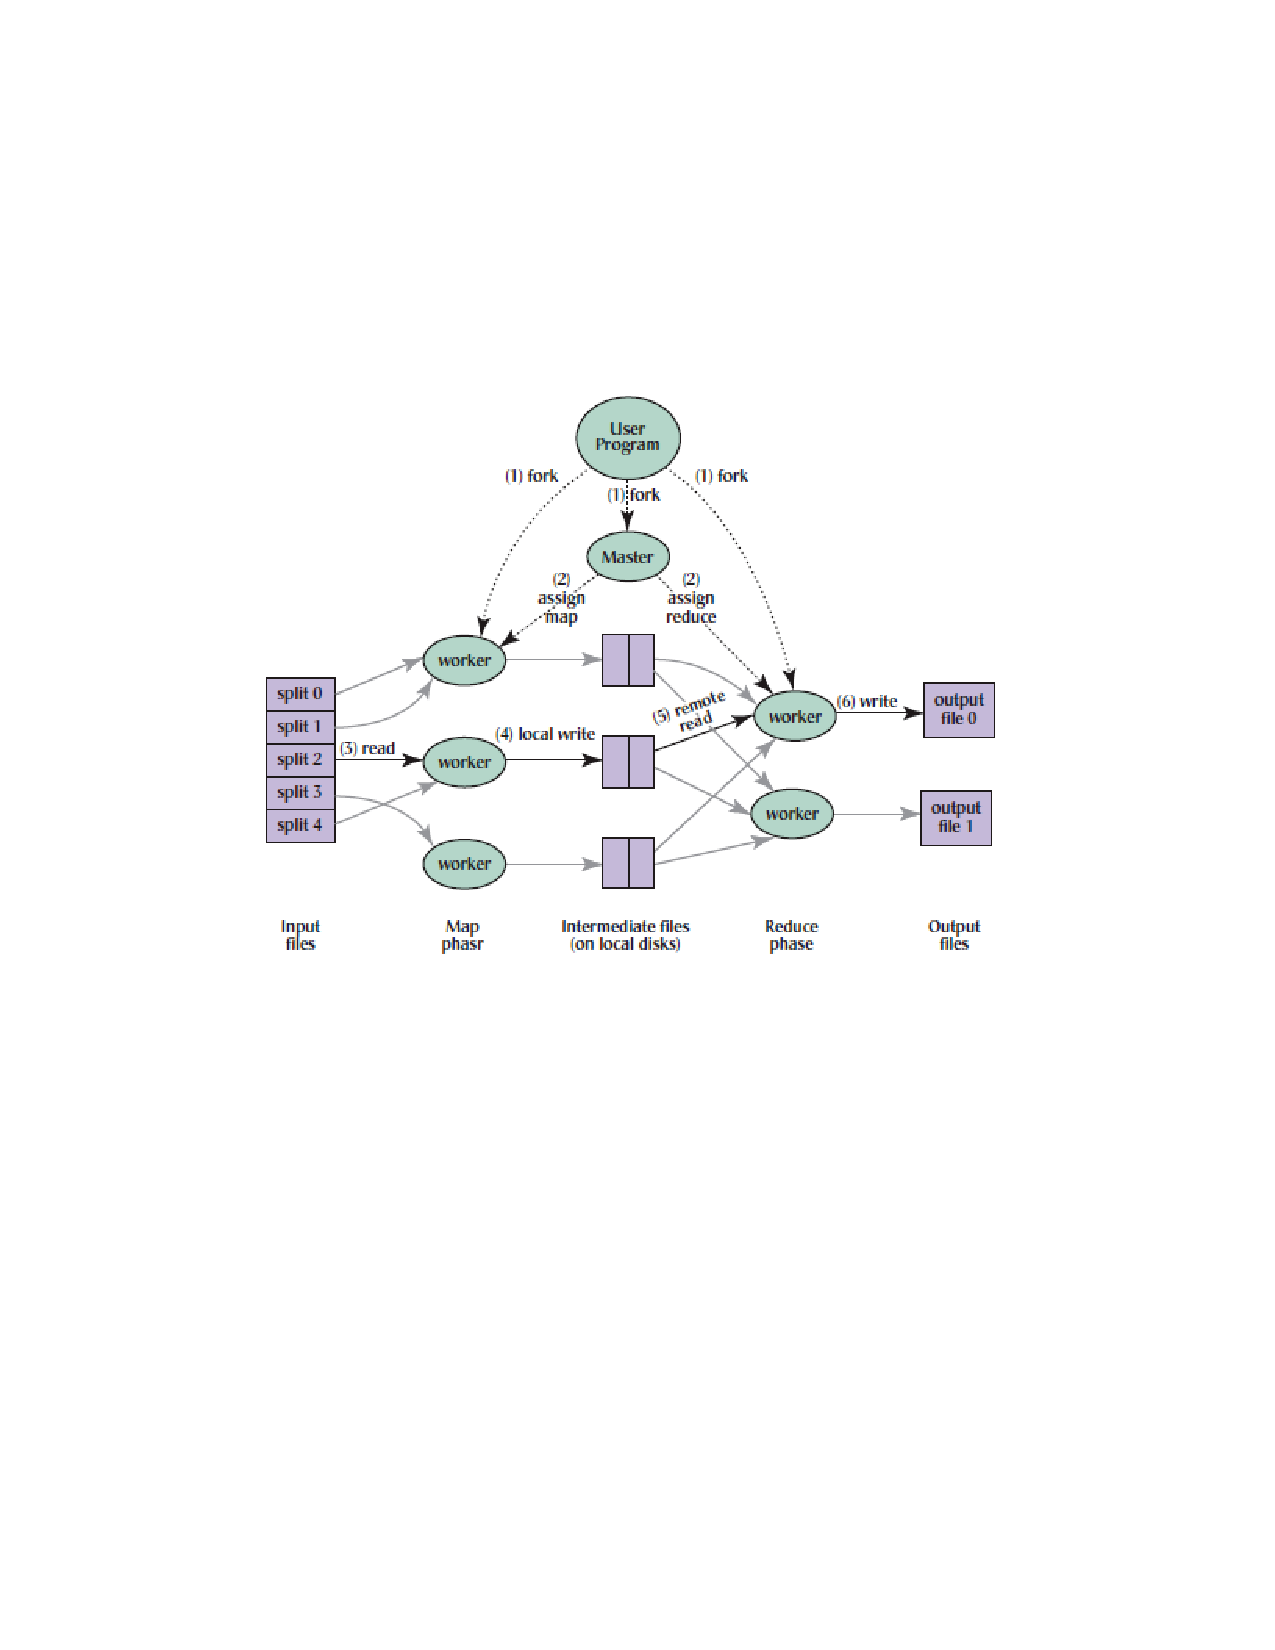
\includegraphics[width=1.0\textwidth]{img/map_reduce_overview.pdf}
  \caption{Overview of the MapReduce program, from \cite{ghemawat:2003}.}
\end{figure}
\end{center}

\subsection{The Hog Language}
\label{sub:hog_language}

Hog is a \textbf{data-oriented}, \textbf{high-level}, scripting language for
creating MapReduce programs. Used alongside Hadoop, Hog enables users to
efficiently carry out \textbf{distributed} computation. Hadoop MapReduce is an
open-source implementation of the MapReduce framework, which is especially useful
for working with large data sets. While it is possible to write code to carry out
computations with Hadoop directly, the framework requires users to specify
low-level details that are often irrelevant to their desired goal.

By building a scripting language on top of Hadoop, we aim to simplify the process.
Built around a \textbf{simple} and highly \textbf{readable} syntax, Hog will let
users focus on what computations they want done, and not how they want to do them.
Hog takes care of all the low-level details required to run computations on
Hadoop’s distributed network. All a user needs to do is tell Hog the location of
their valid Hadoop instance, and Hog will do the rest.

We intentionally have restricted the scope of Hog to deal with specific
problems.  For example, Hog only supports reading and writing plaintext files.
While these limitations sacrifice the generality of the language, they promote
ease of use.

\subsubsection{Guiding Principles} % (fold)
\label{ssub:guiding_principles}

The guiding principles of Hog are:

\begin{itemize}
  \item Anyone can MapReduce
  \item Brevity over verbosity
  \item Simplicity over complexity
\end{itemize}


% subsubsection guiding_princples (end)

\subsection{The ``Ideal'' Hog User} % (fold)
\label{sub:the_ideal_hog_user}

Hog was designed with a particular user in mind: one that has already learned
the basics of programming in a different programming language (such as Java or
Python), but is inexperienced with distributed computation and can benefit from
a highly structured framework for writing MapReduce programs. The language was
designed with the goal of making learning how to write MapReduce programs as
easy as possible. However, the user should be adept with programming concepts
such as program structure, control flow (iteration and conditional operators),
evaluation of boolean expressions, etc.

% subsection the_ideal_hog_user (end)


\section{Syntax Notation} % (fold)
\label{sec:syntax_notation}

In the syntax notation used throughout the Hog manual, different syntactic
categories are noted by \emph{italic type}, and literal words and characters
are in \tt typewriter style\rm. When specific terms are introduced,
\textbf{\emph{emboldened, italicized font}} is used.

% sec syntax_notation (end)

\section{Program Structure} % (fold)
\label{sec:program_structure}

\subsection{Overall Structure} % (fold)
\label{sub:overall_structure}

Every Hog program consists of a single source file with a ‘.hog’ extension. This
source file must contain three sections: \tt @Map\rm, and \tt @Reduce\rm, and
\tt @Main \rm and can also include an optional \tt @Functions \rm section. These
sections must be included in the following order:

\begin{verbatim}
   @Functions {
      .
      .
      .
    }
    @Map <type signature> {
      .
      .
      .
    }
    @Reduce <type signature> {
      .
      .
      .
    }
    @Main {
      .
      .
      .
    }
\end{verbatim}

% section overall_structure (end)

\subsection{\tt @Functions\rm} % (fold)
\label{sub:tt_functionsrm}

At the top of every Hog program, the programmer has the option to define functions
in a section called \tt @Functions\rm. Any function defined in this section can be
called from any other section of the program, including \tt @Map\rm, \tt
@Reduce\rm, and \tt @Main \rm and can also be called from other functions defined
in the \tt @Functions \rm section. The section containing the functions begins
with the keyword \tt @Functions \rm on its own line, followed by the function
definitions.

Function definitions have the form:

\begin{quotation}
  \emph{type functionName} \tt ( \rm \emph{parameterList} \tt ) \{ \rm \\
  \indent \indent \emph{expressionList}; \\
  \indent \tt \}
\end{quotation}

where,

\begin{quotation} \emph{parameterList} $\rightarrow$ \emph{parameter} \tt , \rm
\emph{parameterList} $|$ \emph{parameter} \end{quotation}

The return type can be any valid Hog type. The rules regarding legal function
names are identical to those regarding legal variable identifiers. Each
parameter in the parameter list consists of a valid Hog type followed by the
name of the parameter, which must also follow the naming rules for identifiers.
Parameters in the parameter list are separated by commas. The \tt @Functions
\rm section ends when the next Hog section begins.

A complete example of an \tt @Functions \rm section:

\begin{verbatim}
    @Functions {
      int min(int a, int b) {
        if (a < b) {
          return a;
        } else {
          return b;
        }
      }

      list<int> reverseList(list<int> oldList) {
        list<int> newList;
        for (int i = oldList.size() - 1; i >= 0; i--;) {
          newList.add(oldList.get(i));
        }
        return newList;
      }
    }
\end{verbatim}

User-defined functions can make reference to other user-defined functions.
However, function names cannot be overloaded (i.e. it is not possible to use
the same function name with a parameter list that differs in the number of
arguments or argument types). Disallowing function overloading is a design
choice consistent with Hog's guiding principle of simplicity.

% section tt_functionsrm (end)

\subsection{\tt @Map \rm} % (fold)
\label{sub:tt_map_rm}

The map function in a MapReduce program takes as input key-value pairs, performs
the appropriate calculations and procedures, and emits intermediate key-value
pairs as output. Any given input pair may map to zero, one, or multiple output
pairs. The \tt @Map \rm section defines the code for the map function.

The \tt @Map \rm header must be followed by the signature of the map function, and
then the body of the map function as follows:

\begin{quotation} \tt @Map ( \rm \emph{type identifier, type identifier} \tt )
-> ( \rm \emph{type, type} \tt ) \{ \\ \indent \indent . \\ \indent \indent .
\\ \indent \indent . \\ \indent \tt \} \rm \end{quotation}

The first \emph{type identifier} defines the \emph{\textbf{key}} and the second
defines the \emph{\textbf{value}} of the input key-value pair to the \tt @Map
\rm function. The identifiers specified for the key and value can be made
reference to later within the \tt @Map \rm block. The \tt @Map \rm signature is
followed by an arrow and another key-value pair, defining the types of the
output of the map function. Notice that identifiers are not specified for the
output key and value (said to be \emph{\textbf{unnamed}}), as these pairs are
only produced at the end of the map function. 

The map function can include any number of calls to \tt emit()\rm, which outputs
the resulting intermediate key-value pairs for use by the function defined in the
\tt @Reduce \rm section. The types of the values passed to the \tt emit() \rm
function must agree with the signature of the output key-value pair as defined in
the \tt @Map \rm type signature. All output pairs from the map function are
subsequently grouped by key by the framework, and passed as input to the \tt
@Reduce \rm function.

\emph{Note}: In the current version of the language, the only configuration
available is for a file to be passed into the map function one line at a time,
with the line of text being the value, and the corresponding line number as the
key. This requires that the input key/value pair to the map function is of type
\tt (int key‐name, text value‐name)\rm. Extending this to allow for other input
formats is a future goal of the Hog language.

The following is an example of a complete \tt @Map \rm section for a program that
counts the number of times each word appears in a set of files. The map function
receives a single line of text, and for each word in the line (as delineated by
whitespace), it emits the word as the key with a value of one. By emitting the word
as the key, we can allow the framework to group by the word, thus calling the
reduce function for every word.

\begin{verbatim}

  @Map (int lineNum, text line) -> (text, int) {
      # for every word on this line, emit that word and the number 1
      foreach text word in line.tokenize(" ") {
          emit(word, 1);
       }
   }

\end{verbatim}


% section tt_map_rm (end)

\subsection{\tt @Reduce \rm} % (fold)
\label{sub:tt_reduce_rm}

The reduce function in a MapReduce program takes a list of values that share the
same key, as emitted by the map function, and outputs a smaller set of values to
be associated with another key. The input and output keys do not have to match,
though they often do.

The setup for the reduce section is similar to the map section. However, the input
value for any reduce function is always an iterator over the list of values
associated with its key. The type of the key must be the same as the type of the
key emitted by the map function. The iterator must be an iterator over the type of
the values emitted by the map function.

\begin{quotation}
  \tt @Reduce ( \rm \emph{type identifier, type identifier} \tt ) -> ( \rm \emph{type, type} \tt ) \{ \\
  \indent \indent . \\
  \indent \indent . \\
  \indent \indent . \\
  \indent \tt \} \rm
\end{quotation}

As with the map function, the reduce function can emit as many key/value pairs as
the user would like. Any key/value pair emitted by the reduce function is recorded
in the output file.

Below is a sample \tt @Reduce \rm section, which continues the word count example,
and follows the \tt @Map \rm sample introduced in the previous section.

\begin{verbatim} 

    @Reduce (text word, iter<int> values) -> (text, int) {
      # initialize count to zero
      int count = 0;
      while (values.hasNext()) {
        # for every instance of '1' for this word, add to count
        count = count + values.next();
      }
      # emit the count for this particular word
      emit(word, count);
    }

\end{verbatim} 

% subsection tt_reduce_rm (end)

\subsection{\tt @Main \rm} % (fold)
\label{sec:tt_main_rm}

The \tt @Main \rm section defines the code that is the entry point to a Hog
program. In order to run the MapReduce program defined by the user in the
previous sections, \tt @Main \rm must contain a call to the system-level
built-in function \tt mapReduce() \rm, which calls the \tt @Map \rm and \tt
@Reduce \rm functions. Other arbitrary code can be run from the \tt @Main \rm
section as well. In the current version of the language, \tt @Main \rm does not
have access to the results of the MapReduce program resulting from a call to
\tt mapReduce()\rm. Therefore, it is quite common for the \tt @Main \rm section
to contain the call to \tt mapReduce() \rm and nothing else.

Below is a sample \tt @Main \rm section which prints to the standard output and
runs a map reduce job.

\begin{verbatim}
    @Main {
          print("Starting mapReduce job.\n");
          mapReduce();
          print("mapReduce complete.\n");
    }
\end{verbatim}


% subsection tt_main_rm (end)

% section program_structure (end)

\section{Lexical Conventions} % (fold)
\label{sec:lexical_conventions}

\subsection{Tokens} % (fold)
\label{sub:tokens}

The classes of tokens include the following: identifiers, keywords,
constants, string literals, operators, and separators. Blanks, tabs, newlines, and
comments are ignored. If the input is separated into tokens up to a given
character, the next token is the longest string of characters that could represent
a token.

% subsection tokens (end)

\subsection{Comments} % (fold)
\label{sub:comments}

Multi-line comments are identified by the enclosing character sequences \tt
\#\{ \rm and \tt \}\#\rm. Anything within these enclosing characters is
considered a comment, and is completely ignored by the compiler. For example,

\begin{verbatim}
    int i = 0;
    #{ these are block
        comments and are ignored
         by the compiler }#
    i++;

\end{verbatim}

In the above example, the text \tt these are block comments \textbackslash n
comments and are ignored \textbackslash n by the complier \rm is completely
ignored during compilation. Compilation goes directly from the line \tt int i =
0; \rm to the line \tt i++;\rm.

Single-line comments are defined to be strings of text included between a '\tt
\#\rm' symbol on the left-hand side and a newline character ('\tt\textbackslash
n\rm') on the right-hand side.

% subsection comments (end)

\subsection{Identifiers} % (fold)
\label{sub:identifiers}

A valid identifier in Hog is a sequence of contiguous letters, digits, or
underscores, which are used to distinguish declared entities, such as methods,
parameters, or variables from one another. A valid identifier also provide a
means of determining scope of an entity, and helps to determine whether the
same valid identifier in another scope refers to the same entity. The first
character of an identifier must not be a digit. Valid identifiers are case
sensitive, so \tt foo \rm is not the same identifier as \tt Foo\rm.

% section identifiers (end)

\subsection{Keywords} % (fold)
\label{sub:keywords}

The following words are reserved for use as keywords, and may not be redefined
by the programmer:

\begin{multicols}{4}
\tt
\begin{itemize}
  \item[] add
  \item[] and
  \item[] bool
  \item[] break
  \item[] catch
  \item[] clear
  \item[] contains
  \item[] containsAll
  \item[] continue
  \item[] default
  \item[] else
  \item[] elseif
  \item[] emit
  \item[] final
  \item[] for
  \item[] foreach
  \item[] Functions
  \item[] get
  \item[] hadoop
  \item[] hasNext
  \item[] if
  \item[] in
  \item[] instanceof
  \item[] int
  \item[] int2real
  \item[] int2text
  \item[] isEmpty
  \item[] iter
  \item[] list
  \item[] Map
  \item[] mapReduce
  \item[] next
  \item[] not
  \item[] or
  \item[] peek
  \item[] print
  \item[] real
  \item[] real2int
  \item[] real2text
  \item[] Reduce
  \item[] remove
  \item[] removeAll
  \item[] return
  \item[] size
  \item[] sort
  \item[] text
  \item[] text2int
  \item[] text2real
  \item[] throw
  \item[] tokenize
  \item[] try
  \item[] void
  \item[] while
  
  
\end{itemize}
\rm
\end{multicols}

% subsection keywords (end)

\subsection{Constants} % (fold)
\label{sub:constants}

The word \textbf{\emph{constant}} has two different meanings in Hog. It can
refer to either a variable that is \emph{fixed}, that is, once it is
initialized cannot be changed, or can refer to an \textbf{\emph{unnamed
value}}, such as "1.0". To declare a constant variable, use the following
pattern,

\begin{quotation}
   \tt final \rm \emph{type variableName} = \emph{value};
\end{quotation}

The following are a list of examples of unnamed values and their corresponding
types:

\begin{itemize}
  \item[] \tt -1\rm, \tt 0\rm, \tt 1\rm, \tt 2\rm $\hfill$ (all of type \tt int\rm)
  \item[] \tt -0.12\rm, \tt3.14159\rm, \tt 2.7182\rm, \tt 1.41421 \rm $\hfill$ (all of type \tt real\rm)
  \item[] \tt true\rm, \tt false \rm $\hfill$ (all of type \tt bool\rm)
\end{itemize}

% subsection constants (end)

\subsection{Text Literals} % (fold) \label{sub:string_literals} 

A text literal consists of a sequence of zero of more contiguous characters
enclosed in double quotes, such as \tt "hello"\rm. A text literal can also
contain escape characters such as \tt "\textbackslash n" \rm for the new line
character or \tt "\textbackslash t" \rm for the tab character. A text literal
has many of the same built-in functions as the String class in Java. String
literals are constant and their values cannot be changed after they are
created. String literals can be concatenated with adjacent text literals by use
of the \tt + \rm operator and are then converted into a single \tt text \rm
variable. Hog implements concatenation by use of the Java \tt StringBuilder \rm
(or \tt StringBuffer\rm) class and its append method. All text literals in Hog
programs are implemented as instances of the \tt text \rm class, and then are
mapped directly to the equivalent \tt String \rm class in
Java.\footnote{Technically, \tt text \rm objects are implemented as instances
of Hadoop's \tt Text \rm class, which is closely related to the Java \tt String
\rm class.}

% subsection string_literals (end)

\subsection{Variable Scope} % (fold)
\label{sub:variable_scope}

Hog implements what is generally referred to as lexical scoping or block scope. An
identifier is valid within its enclosing block. The identifier is also valid for
any block nested within its enclosing block.

% subsection variable_scope (end)


\subsection{Argument Passing}
\label{sub:argument_passing}

Since Hog is compiled into Java, it passes arguments using call-by-value.
However, derived types such as \tt list \rm are Object types, and thus
variables are references to that Object's memory location. For these types,
Hog behaves as if it were call-by-reference, since the value of the reference (i.e. the memory location)
is passed to the callee function. This enables the callee to directly manipulate the same object,
even thought it has only received a \emph{copy} of the reference, rather than the original reference
itself.

\subsection{Evaluation Order}
\label{sub:evaluation_order}

Hog uses applicative order (eager) evaluation, similarly to Java. This amounts to evaluating
the parameters to a function call before evaluating the function itself.

% section lexical_conventions (end)


\section{Types} % (fold)
\label{sec:types}

\subsection{Basic Types} % (fold)
\label{sub:basic_types}

The basic types of Hog include \tt int \rm (integer numbers in base 10, 64
bytes in size), \tt real \rm (floating point numbers, 64 bytes in size), \tt
bool \rm(boolean values, \tt true \rm or \tt false \rm) and \tt text \rm
(Strings, variable in size).  Unlike some languages, Hog includes no basic
character type. Instead, a programmer makes use of \tt text\rm s of size 1.

\emph{Implementation details}: Hog’s primitive types are not so primitive. They are
in fact wrappers around Hadoop classes. For instance, Hog’s \tt int \rm type is a
wrapper around Hadoop's \tt IntWritableclass\rm. The following lists for every
primitive type in Hog the corresponding Hadoop class that the type is built on top
of:

\begin{center}
\begin{tabular}{|c|c|}
    \hline
\textbf{Hog Type} & \textbf{Enclosed Hadoop Class} \\ \hline
\tt int & \tt IntWritable \\ \hline
\tt real & \tt DoubleWritable \\ \hline
\t bool & \tt BooleanWrtiable \\ \hline
\tt text & \tt Text \rm \\ \hline
\end{tabular}
\end{center}

% subsection basic_types (end)

\subsection{Derived Types (Collections)} % (fold)
\label{sub:derived_types_collections_}

There are two derived types that can be created by the programmer: \tt
list<T>\rm and \tt set<T>\rm.  Future versions of Hog are expected to implement
other derived types, including dictionaries/hash maps, user-defined iterators,
and multisets. The \tt list<T> \rm type is an ordered collection of objects of
the same type. The \tt set<T> \rm is an unordered collection of unique objects
of the same type. Hog supports arbitrarily nested derived types, so it is
possible, for example, to have a \tt list\rm  of \tt list\rm s of \tt list\rm s
of \tt int\rm s.

A special derived type is \tt iter<T>\rm, which is Hog's iterator object. An
\tt iter \rm object is associated with a list, and allows one traversal of the
elements in the list; this is used by Hog in the \tt @Reduce \rm section of a
Hog program.

% subsection derived_types_collections_ (end)

\subsection{Type Conversions} % (fold)
\label{sub:conversions}

\textbf In order to cast a variable to be of a different type, use the
following notation:

\begin{quotation}
      \tt \emph{primitiveType}(2\emph{otherPrimitiveType})\rm \emph{variableName}
\end{quotation}

Hog supports casting between the primitive types \tt int\rm, \tt real\rm, and
\tt text\rm, via the built-in functions \tt int2real\rm, \tt int2text\rm, \tt
real2int\rm, \tt real2text\rm, \tt text2int\rm, and \tt text2real\rm. If
casting a text to an int or real results in an invalid number (e.g. \tt
text2int("1a4") \rm), a run-time exception will be thrown.

% subsection conversions (end)

% section types (end)

\section{Expressions} % (fold)
\label{sec:expressions}

\subsection{Operators} % (fold)
\label{sub:operators}

\subsubsection{Arithmetic Operators} % (fold)
\label{ssub:arithmetic_operators}

Hog implements all of the standard arithmetic operators. All arithmetic
operators are only defined for use between variables of numeric type (\tt
int\rm, \tt real\rm) with the exception that the \tt + \rm operator is also
defined for use between two \tt text \rm variables. In such instances, \tt +
\rm is defined as concatenation. Thus, in the following,

\begin{verbatim}
    text face = "face";
    text book = "book";
    text facebook = face + book;
\end{verbatim}

After execution, the variable \tt facebook \rm will have the value
``facebook''. No other arithmetic operators are defined for use with \tt text
\rm variables, and \tt + \rm is only valid if both variables are of type \tt
text \rm. Otherwise, the program will result in a compile-time \tt
TypeMismatchException\rm. 

When an arithmetic operator is used between two numeric variables of different
type, as in,

\begin{verbatim}
    int a = 1;
    real b = 2.0;
\end{verbatim}

\noindent the non-\tt real \rm variable would first need to be cast into a \tt
real \rm before operating on them, so that both operands have the
same type. So thus

\begin{verbatim}
   print(a + b);
\end{verbatim}

would throw an error, while

\begin{verbatim}
   print(int2real(a) + b);
\end{verbatim}

would print 3.0.

If one of the operands happens to have a \tt null \rm value (for instance, if a
variable is \textbf{\emph{uninitialized}}), then the resulting operation will
cause a run-time \tt NullValueException\rm, and the program will crash.

\begin{center}
\begin{tabular}{|c|c|c|c|c|}

\hline \textbf{Operator} & \textbf{Arity} & \textbf{Associativity} &
\textbf{Precedence Level} & \textbf{Behavior} \\ \hline
\tt + \rm & binary & left & 0 & addition \\ \hline
\tt - \rm & binary & left & 0 & minus \\ \hline
\tt * \rm & binary & left & 1 & multiplication \\ \hline
\tt / \rm & binary & left & 1 & division \\ \hline
\tt \% \rm & binary & left & 2 & mod$\dagger$
\\ 
\hline
\tt ++ \rm & unary & left & 3 & increment \\ \hline
\tt -- \rm & unary & left & 3 & decrement \\ \hline
\tt - \rm & unary & right & 3 & negate \\ \hline
\end{tabular}
\end{center}

$\dagger$Follows Java's behavior: a modulus of a negative number is a negative
number.
% subsubsection arithmetic_operators (end)

\subsubsection{Logical Operators} % (fold)
\label{ssub:logical_operators}

The following are the logical operators implemented in Hog. Note that these
operators only work with two operands of type \tt bool\rm. Attempting to use a
logical operator with an object of any other type results in a compile-time
exception (see \S \ref{sub:compile_time_exceptions}).

\begin{center}
\begin{tabular}{|c|c|c|c|c|}

\hline \textbf{Operator} & \textbf{Arity} & \textbf{Associativity} &
\textbf{Precedence Level} & \textbf{Behavior} \\ \hline
\tt or \rm & binary & left & 0 & logical or \\ \hline
\tt and \rm & binary & left & 1 & logical and \\ \hline
\tt not \rm & unary & right & 2 & negation \\ \hline
\end{tabular}
\end{center}

% subsubsection logical_operators (end)

\subsubsection{Comparators} % (fold)
\label{ssub:comparators}

The following are the comparators implemented in Hog (all are binary operations).

\begin{center}
\begin{tabular}{|c|c|c|c|}

\hline \textbf{Operator} & \textbf{Associativity} &
\textbf{Precedence Level} & \textbf{Behavior} \\ \hline
\tt < \rm & none & 0 & less than \\ \hline
\tt <= \rm & none & 0 & less than or equal to \\ \hline
\tt > \rm & none & 0 & greater than \\ \hline
\tt >= \rm & none & 0 & greater than or equal to \\ \hline
\tt == \rm & none & 0 & equal \\ \hline
\tt != \rm & none & 0 & not equal \\ \hline

\end{tabular}
\end{center}

\emph{Note}: All comparators do not work with non-numeric or non-boolean types.
Comparisons require that the two operands be either both numeric or both
boolean, and a numeric value cannot be compared to a boolean value. If the two
operands are numeric but of different types, one of them must be cast so that
they are of the same type. The only valid comparators that can be used with
boolean expressions are \tt == \rm and \tt !=\rm. The use of a comparison
operator in Hog between any two derived types will result in a run-time error.

% subsubsection comparators (end)

\subsubsection{Assignment} % (fold)
\label{ssub:assignment}

There is one assignment operator, '\tt =\rm'. Expressions involving the
assignment operator have the following form:

\begin{quotation}
\emph{identifier}$_1$ \tt = \rm \emph{expression} $|$ \emph{identifier}$_2$
\end{quotation}

At compile time, the compiler checks that both the result of the \emph{expression}
(or \emph{identifier}$_2$) and \emph{identifier}$_1$ have the same type. If not, a
compile-time \tt TypeMismatchException \rm will be thrown.

% subsubsection assignment (end)

% subsection operators (end)

% section expressions (end)

\section{Declarations} % (fold)
\label{sec:declarations}

A user is only allowed to use variables/functions after they have been
declared. When declaring a variable, a user must include both a type and an
identifier for that variable. Otherwise, an exception will be thrown at compile
time.

\subsection{Type Specifiers} % (fold)
\label{sub:type_specifiers}

Every variable, whether its type is primitive or derived, must be assigned a
type upon declaration, for instance,

\begin{verbatim}
    list<int> myList;
\end{verbatim}

declares the variable \tt myList \rm to be a \tt list \rm of \tt int\rm s,

\begin{verbatim}
    list<list<int>> myOtherList;
\end{verbatim}

declares the variable \tt myOtherList \rm to be a \tt list \rm of \tt list\rm s
of \tt int \rm s,

and

\begin{verbatim}
    text myText;
\end{verbatim}

declares the variable \tt myText \rm to be of type \tt text\rm .

% subsection type_specifiers (end)

\subsection{Declarations} % (fold)
\label{sub:declarations}

\subsubsection{Null Declarations} % (fold)
\label{ssub:null_declarations}

If a variable is declared but not initialized, the variable becomes a
\textbf{\emph{null reference}}, which means it points to nothing and holds no
data (internally, this means that an entry has been added to Hog's symbol table
with that variable name).

% subsubsection null_declarations (end)

\subsubsection{Primitive-Type Variable Declarations} % (fold)
\label{ssub:primitive_type_variable_declarations}

Variables of one of the primitive types, including \tt int\rm, \tt real\rm, \tt
text\rm, or \tt bool\rm, are declared using the following patterns:

\begin{enumerate}
  \item \emph{type identifier} \rm $\hfill$ (uninitialized)
  \item \emph{type identifier = expression } \rm $\hfill$ (initialized)
\end{enumerate}

When the first pattern is used, we say that the variable is
\textbf{\emph{uninitialized}}, and has the value \tt null\rm. When the second
pattern is used, we say that the variable is \textbf{\emph{initialized}}, and has
the same value as the value of the result of the \emph{expression}. The
\emph{expression} must return a value of the right type, or the compiler will
throw a \tt TypeMismatchError\rm. The \emph{expression} may contain an expression
involving both other variables and unnamed raw primitives (e.g. 1 or 2), an
expression involving only other variables or unnamed raw primitives, or a single
variable, or a single unnamed raw primitive.

% subsubsection primitive_type_variable_declarations (end)

\subsubsection{Derived-Type Variable Declarations} % (fold)
\label{ssub:derived_type_variable_declarations}

Derived-type variables are declared using the following pattern:

\begin{enumerate}
  \item \emph{type identifier;}
\end{enumerate}

When the derived type is first declared, we say that the variable is
\textbf{\emph{uninitialized}}, and has the value \tt null\rm. If a user
attempts to use any type-­specific operations that are not meaningful (for
instance, \tt myList.size() \rm on an uninitialized variable, the program will
throw a run­time exception (see \S \ref{sec:exception_handling} for a
discussion of exceptions)). The example code below initializes a \tt list\rm of
integers and adds one element to it.

\begin{verbatim}
    list<int> myList;
    myList.add(5);
\end{verbatim}

% subsubsection derived_type_variable_declarations (end)

\subsubsection{Function Declarations} % (fold)
\label{ssub:function_declarations}

In order to declare a function, use the following notation:

\begin{quotation}
\emph{type functionName} \tt ( \rm \emph{parameterList} \tt ) \{ \rm \\
\indent \indent \emph{expressionList} \\
\indent \tt \}
\end{quotation}


% subsubsection function_declarations (end)

% subsection declarations (end)

% section declarations (end)

\section{Statements} % (fold)
\label{sec:statements}

\subsection{Expression Statement} % (fold)
\label{sub:expression_statement}

An \textbf{\emph{expression statement}} is either an individual assignment or a
function call. All consequences of a given expression take effect before the next
expression is executed.

% subsection expression_statement (end)

\subsection{Compound Statement (Blocks)} % (fold)
\label{sub:compound_statement}

\textbf{\emph{Compound statements}} are defined by \{ and \} and are used to
group a sequence of statements, so that they are syntactically equivalent to a
single statement.

% subsection compound_statement (end)

\subsection{Flow-Of-Control Statements} % (fold)
\label{sub:flow_of_control_statements}

The following are the \textbf{\emph{flow-of-control}} statements included in Hog:

\begin{itemize}
  \item[] \tt if ( \rm \emph{expression} \tt ) \rm \emph{statement}
  \item[] \tt if ( \rm \emph{expression} \tt ) \rm \emph{statement} \tt else \rm \emph{statement}
  \item[] \tt if ( \rm \emph{expression} \tt ) \rm \emph{statement} \tt elseif ( \rm \emph{statement} \tt ) $\dots$ else 
  \rm \emph{statement}
\end{itemize}

In the above statements, the  $\dots$ signifies an unlimited number of \tt
elseif \rm statements, since there is no limit on the number of \tt elseif \rm
statements that can appear before the final \tt else \rm statement. In the
second statement above, when the expression in the \tt if \rm statement
evaluates to \tt false\rm, then the \tt else \rm statement will execute. In the
third statement above with \tt if\rm, \tt elseif \rm and \tt else \rm
statements, the statement will be executed that follows the first expression
evaluating to \tt true\rm. If none of these expressions evaluate to \tt
true\rm, then the \tt else \rm statement is executed.

To increase the expressive power of Hog, flow-of-control statements can also be
nested within each other.

% subsection flow_of_control_statements (end)

\subsection{Iteration Statements} % (fold)
\label{sub:iteration_statements}

Iteration statements signify looping and can appear in one of the two following
forms:

\begin{itemize}
  \item[] \tt while ( \rm \emph{expression} \tt ) \rm \emph{statement}
  \item[] \tt for ( \rm \emph{expression}$_1$ \tt ; \rm \emph{expression}$_2$ \tt ; \rm \emph{expression}$_3$ \tt ;) \rm \emph{statement}
  \item[] \tt foreach \rm \emph{expression} \tt in \rm \emph{iterable-object statement}
\end{itemize}

In the \tt while \rm pattern, the associated \emph{statements} will be executed
repeatedly until the \emph{expression} evaluates to \tt false\rm. The
\emph{expression} is evaluated before every iteration. Please note that in a
slight syntactical departure from Java, Hog requires a semicolon after the
third expression (the increment step) in the \tt for\rm loop construct. Thus,
an example of correct Hog syntax would be \begin{verbatim} for (int i = 0; i <
10; i++;){...}\end{verbatim}

In the \tt for \rm pattern, \emph{expression}$_1$ is the initialization step,
\emph{expression}$_2$ is the test or condition and \emph{expression}$_3$ is the
increment step. At each step through the for loop, \emph{expression}$_2$ is
evaluated. When \emph{expression}$_2$ evaluates to false, iteration through the
loop ends.

In the \tt foreach \rm pattern, the iteration starts at the first element in the
\emph{iterable-object statement} (a statement that evaluates to an object that
supports the \tt iterator() \rm function). The \emph{statement} executes during
every iteration. The iteration ends when the \emph{statement} has been executed
for each item in the iterable object and there are no items left to iterate
through.

\subsubsection{Example of \tt while \rm} % (fold)
\label{ssub:example_1}

\begin{verbatim}
    int i = 0;
    while (i < 10) {
      print(i);
      i++;
    }

\end{verbatim}

% subsubsection example_1 (end)

\subsubsection{Example of \tt for \rm} % (fold)
\label{ssub:example_2}

\begin{verbatim}
    for (int i = 0; i < 10; i++;) {
      print(i)
    }
\end{verbatim}

% subsubsection example_2 (end)

\subsubsection{Example of \tt foreach \rm} % (fold)
\label{ssub:example_3}

\begin{verbatim}
    # we first initialize and populate the list as follows: 
    list<int> iList;
    for (int i = 0; i < 10; i++;) {
       iList.add(i);
    }

    # This is an example of using foreach
    # Note that the type of the iterable must be declared.    

    foreach int i in iList {
      print(i);
    }
\end{verbatim}

% subsubsection example_3 (end)

% subsection iteration_statements (end)

% section statements (end)

\section{Built-in Functions} % (fold)
\label{sec:built_in_functions}

Hog includes both \emph{\textbf{system-level}} and \emph{\textbf{object-level}}
built-in functions. Here \emph{\textbf{built-in}} means functions provided by the
language itself.

\subsection{System-level Built-ins} % (fold)
\label{sub:system_level_built_ins}

Hog includes a number of system­level built­in functions that can be called from
various sections of a Hog program. The functions are:

\begin{itemize} 

\item[] \tt void emit(key, value) \rm \\

This function can be called from the \tt @Map \rm and \tt @Reduce \rm sections in
order to communicate the results of the map and reduce functions to the Hadoop
platform. The types of the key/value pairs must match those defined as the output
types in the header of each section.

\item[] \tt void mapReduce() \rm \\

This function can be called from the \tt @Main \rm section in order to initiate
the mapreduce job, as definied in the \tt @Map \rm and \tt @Reduce \rm sections.
Any Hog program that implements mapreduce will need to call this function in \tt
@Main\rm.

\item[] \tt void print(toPrint) \rm \\

This function can be called from the \tt @Main \rm section in order to print to
standard output. The argument must be a primitive type.

\end{itemize}

% subsection system_level_built_ins (end)

\subsection{Object-level Built-ins} % (fold)
\label{sub:object_level_built_ins}

The derived type objects have several built-in functions that provide
additional functionality. All of these functions are invoked using the
following pattern:

\begin{quotation}
\emph{identifier.functionName(parameterList)}
\end{quotation}

\noindent Where \emph{identifier} is the identifier for the object in question,
\emph{functionName} is the name of the function, and \emph{parameterList} is a
(possibly empty) list of parameters used to specify the behavior of the
invocation.

\emph{Note}: In what follows, if a function has return type T, it means that
the return type of this function matches the parameterized type of this object
(i.e. for an \tt iter<int> \rm object, these functions have return type \tt
int\rm).

\subsubsection{\tt iter \rm} % (fold)
\label{ssub:iter}

\tt iter \rm is Hog's iteration object, and supports several built-in functions
that are independent of the particular type of the \tt iter \rm object. The
built-in functions are as follows:

\begin{itemize}

\item[] \tt bool hasNext() \rm

This function returns \tt true \rm if the iterator object has a next object
to return, and \tt false \rm otherwise.

\item[] \tt T next() \rm

This function returns the next object (if one exists) for the owning \tt iter \rm
object. A call to \tt next() \rm differs from a call to \tt peek() \rm in that the
function call advances the cursor of the iterator.

\item[] \tt T peek() \rm

This function returns the next object (if one exists) for the owning \tt iter
\rm object. A call to \tt peek() \rm returns the object without advancing the
iterator's cursor, thus multiple calls to \tt peek() \rm without any
intermediate function calls will all return the same value.

\end{itemize} 


% subsubsection iter (end)

\subsubsection{\tt list \rm} % (fold)
\label{ssub:list}

\begin{itemize}

\item[] \tt void add(T itemToAdd) \rm

Adds the object passed to the end of the list. The object must be of the same
type as the list, or the operation will result in a \textbf{compile-time or
run-time} exception.

\item[] \tt void clear() \rm

Removes all elements in this \tt list\rm.

\item[] \tt T get(int index) \rm

Returns the item from the list at the specified index.


\item[] \tt void sort() \rm

Function that sorts the items in the list in lexicographical ascending order.

\item[] \tt int size() \rm

Returns an int with the number of elements in the list.

\end{itemize}


% subsubsection list (end)

\subsubsection{\tt set \rm} % (fold)
\label{ssub:tt_set_rm}

\begin{itemize}

\item[] \tt bool add(T element) \rm

Returns \tt true \rm if the element was successfully added to the \tt set\rm, \tt false \rm otherwise.

\item[] \tt void clear() \rm

Removes all elements from the \tt set \rm such that it is empty afterwards.

\item[] \tt bool contains(T element) \rm

Returns \tt true \rm if the \tt set \rm contains this element, \tt false \rm otherwise.

\item[] \tt bool containsAll(set<T> otherSet) \rm

Returns \tt true \rm if all elements in \tt otherSet \rm are found in this set.

\item[] \tt bool isEmpty() \rm

Returns \tt true \rm if there are no elements in this \tt set\rm, \tt false \rm otherwise.

\item[] \tt iter<T> iterator() \rm

Returns an iterator over the elements in this \tt set\rm.

\item[] \tt bool remove(T element) \rm

Returns \tt true \rm if the element was successfully removed from the \tt set\rm, \tt false \rm otherwise (i.e. the \tt list
\rm didn't contain \tt element\rm).

\item[] \tt bool removeAll(set<T> otherSet) \rm

Returns \tt true \rm if all the elements in \tt otherSet \rm were successfully removed from this set.

\item[] \tt int size() \rm

Returns the number of elements in the set.

\end{itemize}

% subsubsection tt_set_rm (end)

\subsubsection{text} % (fold)
\label{ssub:text}

The following function can be called on a \tt text \rm object:

\begin{itemize}

\item[] \tt int length() \rm \\

Returns the length (number of individual characters) of this \tt text\rm.

\item[] \tt text replace(text matchText, text replacementText) \rm \\

Returns a new \tt text \rm object with each sub-\tt text \rm that matches \tt
matchText \rm replaced by \tt replacementText\rm. This function does \textbf{not}
alter the original \tt text \rm object.

\item[] \tt list<text> tokenize(text delimiter) \rm \\

\tt tokenize() \rm can be called on a \tt text \rm object to tokenize it into a
list of \tt text \rm objects based on the delimiter. The delimiter is not included
in any of the \tt text \rm objects in the returned list.

\end{itemize}

% subsubsection text (end)

% subsection object_level_built_ins (end)

% section built_in_functions (end)

\section{System Configuration} % (fold)
\label{sec:system_configuration}

The user must set configuration variables in the \tt hog.rb \rm build script to
allow the Hog compiler to link the Hog program with the necessary jar files to run
the MapReduce job. The user must also specify the job name within the Hog source
file.

\begin{itemize}

\item[] \textbf{HADOOP\_HOME} absolute path of hadoop folder
\item[] \textbf{HADOOP\_VERSION} hadoop version number
\item[] \textbf{JAVA\_HOME} absolute path of java executable
\item[] \textbf{JAVAC\_HOME} absolute path of javac executable
\item[] \textbf{HOST} where to job is rsynced to and run
\item[] \textbf{LOCALMEM} how much memory for java to use when running in local mode 
\item[] \textbf{REDUCERS} the number of reduce tasks to run, set to zero for map only jobs

\end{itemize}

% section system_configuration (end)

\section{Compilation Structure} % (fold)
\label{sec:parsing_tools}

Currently, the Hog compiler is implemented as a translator into the Java
programming language. The first phase of Hog compilation uses the JFlex as its
lexical analyzer, which is designed to work with the Look-Ahead Left-to-Right
(LALR) parser generator CUP. The lexical analyzer creates lexemes, which are
logically meaningful sequences, and for each lexeme the lexical analyzer sends
to the LALR parser a token of the form \tt $<$token-name,
attribute-value$>$\rm. The second phase of Hog compilation uses Java CUP to
create a syntax tree, which is a tree-like intermediate representation of the
source program, which depicts the grammatical structure of the Hog source
program.

In the last phase of compilation, the Hog semantic analyzer generates Java source
code, which is then compiled into byte code by the Java compiler. Then with the
Hadoop Java Archives (JARs) the bytecode is executed on the Java Virtual Machine
(JVM). With the syntax tree and the information from the symbol table, the Hog
compiler then checks the Hog source program to ensure semantic consistency with
the language specification. The syntax tree is initially untyped, but after
semantic analysis Hog types are added to the syntax tree. Hog types are
represented in two ways, either a translation of a Hog type into a new Java class,
or by mapping Hog types to the equivalent Java types. Mapping Hog types directly
to Java types improves performance because a JVM can handle primitive types much
more efficiently than objects. Also, a JVM implements optimizations for well-known
types, such as String, and thus Hog is built for optimal performance.

% section parsing_tools (end)

\section{Linkage and I/O} % (fold)
\label{sec:linkage_and_i_o}

\begin{center}
\begin{figure}
  \label{fig:hog_compiler}
  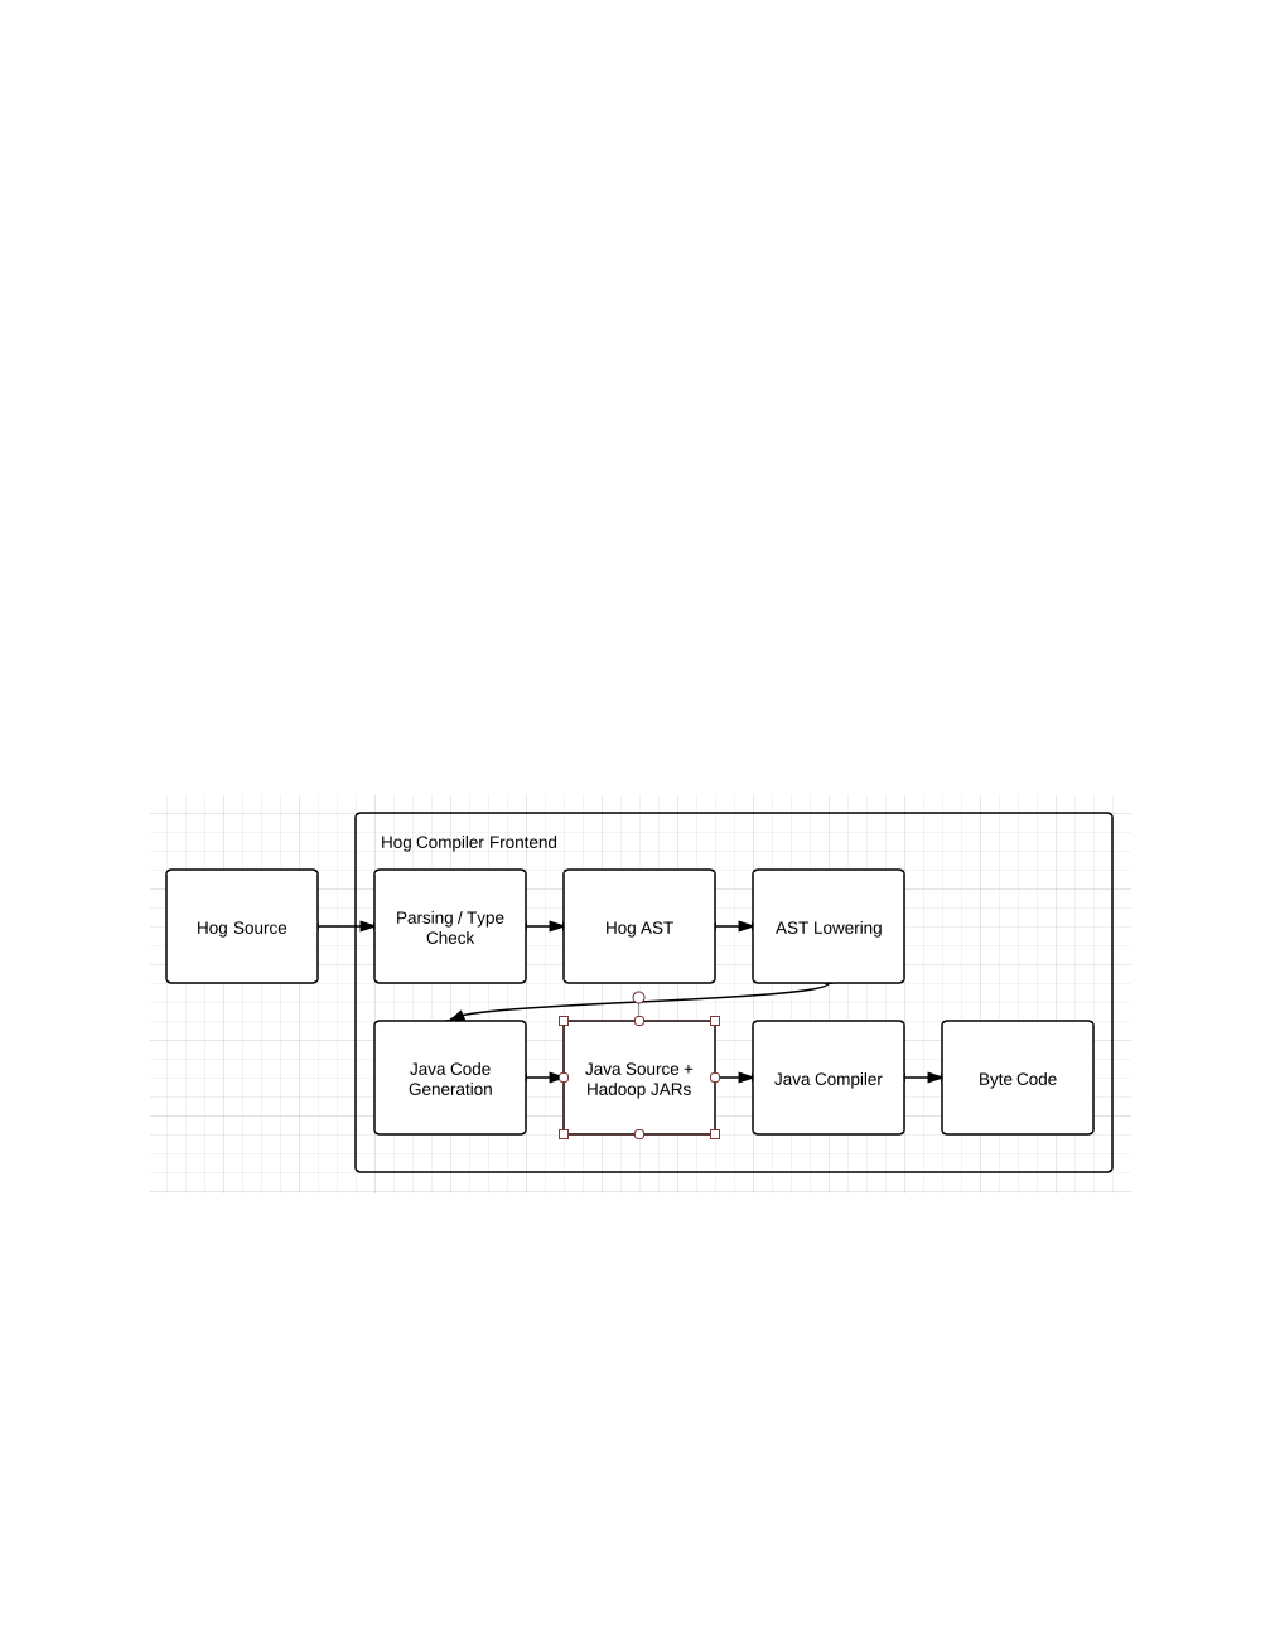
\includegraphics[width=1.0\textwidth]{img/hog_compiler.pdf}
  \caption{The overall structure of the Hog compiler.}
\end{figure}
\end{center}

\subsection{Usage} % (fold)
\label{sub:usage}

% subsection usage (end)

To build and run a Hog source file there is an executable script \tt hog
\rm that automates the compilation and linking steps for the user. \\

Usage: \tt hog [--hdfs|--local] job <job args> \rm
\begin{itemize}
  \item[] \tt --hdfs\rm: if job ends in '.hog' or '.java' and the file exists, link it against the hadoop JARFILE and then run it on HOST.
  \item[] \tt --local\rm: run on local host.
\end{itemize}

\subsection{Example} % (fold)
\label{sub:example}

\begin{verbatim}
hog --local WordCountJob.hog --input someInputFile.txt --output ./someOutputFile.csv
\end{verbatim}

This runs the \tt wordCount \rm job in \emph{local} mode (i.e. not on a Hadoop
cluster).

% subsection example (end)

% section linkage_and_i_o (end)

\section{Exception Handling} % (fold)
\label{sec:exception_handling}

Similar to some other programming languages (such as Java and C++), Hog uses an
exception model in which an exception is thrown and can be caught by a catch
block. Code should be surrounded by a try block and then any exceptions
occurring within the try block will subsequently be caught by the catch block.
Each try block should be associated with at least one catch block. However,
there can be multiple catch blocks to handle specific types of exceptions. In
addition, an optional finally block can be added. The finally block will
execute in all circumstances, whether or not an exception is thrown. The
structure of exception handling should be similar to this, although there can
be multiple catch blocks and the finally block is optional:

\begin{quotation}
\tt try \{ \rm \\
\indent \indent \emph{expression;} \\
\tt \indent \} catch ( \rm \emph{exception} \tt ) \rm \{ \\
\indent \indent \emph{expression;} \\
\tt \indent \} finally \rm \{ \\
\indent \indent \emph{expression;} \\
\tt \indent \}
\end{quotation}

The current version of the language does not support the programmer throwing
exceptions, only catching them.

Because the proper behavior of a Hog program is dependent on resources outside of
the language (i.e. the proper behavior of the user’s Hadoop software), there are
more sources exceptions in Hog than most general purpose languages. These sources
can be divided into two categories: \textbf{\emph{compile­-time exceptions}} and
\textbf{\emph{internal run­-time exceptions}}.

\subsection{Compile-time Errors} % (fold)
\label{sub:compile_time_exceptions}

The primary cause of most compile-­time exceptions in Hog are semantic errors. Such
errors are unrecoverable because it is impossible for the compiler to properly
interpret the user program. Some compilers for other languages offer a limited
amount of compile-­time error correction. Because Hog programs are often designed
to process gigabytes or terabytes of data at a time, the standard Hog compiler
offers no compile-­time error correction. The assumption is that a user would
rather re­tool their program than risk the chance of discovering, only after hours
of processing, that the compilers has incorrectly assumed what the user meant. The
following are Hog compile-­time exceptions:

\begin{itemize}
  
  \item[] \tt FunctionNotDefinedError \rm
  
   Thrown when a program attempts to carry out an operations of the sort \tt
variable.builtInFunction() \rm where \tt variable \rm is some variable and \tt
builtInFunction \rm is a built-in function, and either \tt builtInFunction \rm
cannot operate on variables of that type or \tt builtInFunction \rm  is not
defined as a built-in function.
  
  \item[] \tt InvalidFunctionArgumentsError \rm
   
    Thrown when a program calls a function with the wrong number or type of
parameters. For example, if we define the function \tt max(int a, int b) \rm,
this error will be thrown if the program contains a construct like \tt
max(2,3,4) \rm or \tt max("hello", 3) \rm.

   \item[] \tt TypeMismatchError \rm  

   Thrown when a program attempts to carry out an operation on a variable of
the wrong type (like adding a \tt text \rm and an \tt int \rm together).
  
   \item[] \tt UnreachableCodeError \rm

   Thrown when code is included in a part of a program that will never be
executed (e.g. code after a return statement that can never be reached).

\end{itemize}

% subsection compile_time_exceptions (end)

\subsection{Internal Run-time Exceptions} % (fold)
\label{sub:internal_run_time_exceptions}

Internal run­time exceptions include such problems as I/O exceptions (i.e. a
specified file is not found on either the user’s local file system or the
associated Hadoop file system), type mismatch exceptions (i.e. a program
attempts to place two elements of different types into the same list) and
parsing exceptions. The following are Hog internal run-­time exceptions:


\begin{itemize}
  \item[] \tt FileNotFoundException \rm
  
  Thrown when the the Hog program attempts to open a non-existent file.
  
  \item[] \tt FileLoadException \rm
  
  Thrown when an error occurs while Hog is attempting to read a file (e.g. the
file is deleted while reading).
  
  \item[] \tt ArrayOutOfBoundsException \rm
  
  Thrown when a program tries to access a non-valid index of a \tt list\rm.
  
  \item[] \tt IncorrectArgumentException \rm
  
  Thrown when a derived-type object is instantiated with invalid parameters, or
a function is called with invalid parameters.
  
  \item[] \tt TypeMismatchException \rm
  
  Thrown when a program attempts to carry out an operation on a variable of the
wrong type (like adding a \tt text \rm and an \tt int \rm together).
    
  \item[] \tt NullReferenceException \rm
  
  Thrown whenever the value of a variable cannot be \tt null \rm (e.g. in \tt
myList.get(i)\rm, if \tt i \rm is \tt null\rm, the operation with throw a \tt
NullPointerException\rm).
  
  \item[] \tt ArithmeticException \rm
  
  Thrown whenever an arithmetic operation is attempted on non-numeric operands.
  
\end{itemize}

% section internal_run_time_exceptions (end)

% section exception_handling (end)

\section{Grammar} % (fold)
\label{sec:grammar}

\emph{Note}: The presented grammar has one minor ambiguity relating to the
\textbf{\emph{dangling-else}} problem. If the grammar is run through the parser
generator \tt yacc\rm, \tt yacc \rm will identify 7 shift/reduce parsing-action
conflicts. However, the ambiguity is handled by the default behavior of \tt
yacc\rm, which preferences shift to reduce, associating \tt else \rm and \tt
elseif \rm clauses with the closest \tt if \rm clause.


\begin{verbatim}
terminal DECR, INCR, RETURN, CONTINUE;
terminal TIMES, DIVIDE, MOD;
terminal LESS, GRTR, LESS_EQL, GRTR_EQL, DBL_EQLS, NOT_EQLS, ASSIGN;
terminal TEXT, BOOL, INT, REAL, VOID;
terminal MINUS, UMINUS, PLUS;
terminal ARROW, DOT;
terminal String TEXT_LITERAL;
terminal String ID;
terminal String INT_CONST;
terminal String REAL_CONST;
terminal String BOOL_CONST;
terminal String CASE;
terminal BREAK, DEFAULT;
terminal AND, OR, NOT;
terminal WHILE, FOR, FOREACH, IN, IF, ELSE, ELSEIF, SWITCH;
terminal FUNCTIONS, MAIN, MAP, REDUCE;
terminal L_BRACE, R_BRACE, L_BRKT, R_BRKT, L_PAREN, R_PAREN, SEMICOL, COL, COMMA;
terminal LIST, ITER, SET;
terminal TRY, CATCH, FINALLY;
terminal ExceptionTypeNode EXCEPTION;

nonterminal GuardingStatementNode GuardingStatement;
nonterminal CatchesNode Catches;
nonterminal IdNode CatchHeader;
nonterminal StatementListNode Finally;
nonterminal StatementListNode Block;
nonterminal StatementListNode ExpressionStatements;
nonterminal ExpressionNode ForExpr;
nonterminal StatementListNode ForInit;
nonterminal StatementListNode ForIncr;
nonterminal DerivedTypeNode DictType;

nonterminal ProgramNode Program;
nonterminal SectionNode Functions;
nonterminal SectionNode Main;
nonterminal SectionNode Map;
nonterminal SectionNode Reduce;
nonterminal SectionTypeNode SectionType;
nonterminal StatementNode Statement;
nonterminal ExpressionNode ExpressionStatement;
nonterminal StatementNode FunctionList;
nonterminal StatementNode IterationStatement;
nonterminal StatementNode LabeledStatement;
nonterminal SelectionStatementNode SelectionStatement;
nonterminal StatementNode DeclarationStatement;
nonterminal StatementListNode StatementList;
nonterminal ElseIfStatementNode ElseIfStatement;
nonterminal ElseStatementNode ElseStatement;
nonterminal JumpStatementNode JumpStatement;
nonterminal ExpressionNode EqualityExpression;
nonterminal ExpressionNode LogicalExpression;
nonterminal ExpressionNode LogicalTerm;
nonterminal ExpressionNode RelationalExpression;
nonterminal ExpressionNode Expression;
nonterminal ExpressionNode AdditiveExpression;
nonterminal ExpressionNode MultiplicativeExpression;
nonterminal ExpressionNode CastExpression;
nonterminal ExpressionNode UnaryExpression;
nonterminal ExpressionNode PostfixExpression;
nonterminal ExpressionNode PrimaryExpression;
nonterminal ExpressionNode Constant;
nonterminal ExpressionNode ArgumentExpressionList;
nonterminal FunctionNode Function;
nonterminal ParametersNode ParameterList;
nonterminal TypeNode Type;
nonterminal UnOpNode.OpType UnaryOperator;
nonterminal Types.Derived DerivedType;

precedence left MINUS, PLUS;
precedence right UMINUS;
precedence right ELSE;
precedence right ELSEIF;
precedence right L_PAREN;

start with Program;

Program::=
    Functions Map Reduce Main
  ;

Functions::=
    FUNCTIONS L_BRACE FunctionList R_BRACE
  |
    /* epsilon */
  ; 
 
FunctionList::=
    Function
  |
    FunctionList Function
  ;

Function::=
    Type ID L_PAREN ParameterList R_PAREN L_BRACE StatementList R_BRACE
  ;

ParameterList::=
    ParameterList COMMA Type ID
  |
    Type ID
  |
    /* epsilon */
  ;

Map::=
    MAP SectionType L_BRACE StatementList R_BRACE
  ;

Reduce::=
    REDUCE SectionType L_BRACE StatementList R_BRACE
  ;

SectionType::=
    L_PAREN Type ID COMMA Type ID R_PAREN ARROW L_PAREN Type COMMA Type R_PAREN
  ;

Main::=
    MAIN L_BRACE StatementList R_BRACE
  ;

StatementList::=
    Statement
  |
    StatementList Statement
  ;

Statement::=
    ExpressionStatement
  |
    SelectionStatement
  |
    IterationStatement
  |
    LabeledStatement
  |
    JumpStatement
  | 
    DeclarationStatement
  | 
    GuardingStatement
  | 
    Block
  ;

GuardingStatement::=
     TRY Block Finally
   |
     TRY Block Catches
   | 
     TRY Block Catches Finally
   ;

Block::=
    L_BRACE StatementList R_BRACE
  | 
    L_BRACE R_BRACE
  ;

Finally::=
    FINALLY Block
  ;

Catches::=
     CatchHeader Block
   | 
     Catches CatchHeader Block
   ;

CatchHeader::=
     CATCH L_PAREN EXCEPTION ID R_PAREN
   ;
 
DeclarationStatement::=
    Type ID
  |
    Type ID ASSIGN Expression
  ;
 
JumpStatement::=
    CONTINUE
  |
    BREAK
  |
    RETURN ExpressionStatement
  ;
 
ExpressionStatement::=
    SEMICOL
  |
    Expression SEMICOL
  ;

Expression::=
    LogicalExpression
  |
    UnaryExpression ASSIGN Expression
  ;

LogicalExpression::=
    LogicalExpression OR LogicalTerm
  |
    LogicalTerm
  ;

LogicalTerm::=
    LogicalTerm AND EqualityExpression
  |
    EqualityExpression
  ;

EqualityExpression::=
    RelationalExpression
  |
    EqualityExpression DBL_EQLS RelationalExpression
  |
    EqualityExpression NOT_EQLS RelationalExpression
  ;

RelationalExpression::=
    AdditiveExpression
  |
    RelationalExpression LESS AdditiveExpression
  |
    RelationalExpression GRTR AdditiveExpression
  |
    RelationalExpression LESS_EQL AdditiveExpression
  |
    RelationalExpression GRTR_EQL AdditiveExpression
  ;

AdditiveExpression::=
    MultiplicativeExpression
  |
    AdditiveExpression PLUS MultiplicativeExpression
  |
    AdditiveExpression MINUS MultiplicativeExpression
  ;

MultiplicativeExpression::=
    CastExpression
  |
    MultiplicativeExpression TIMES CastExpression
  |
    MultiplicativeExpression DIVIDE CastExpression
  |
    MultiplicativeExpression MOD CastExpression
  ;

CastExpression::=
    UnaryExpression
  |
    L_PAREN Type R_PAREN CastExpression
  ;

UnaryExpression::=
    UnaryOperator CastExpression
  |
    PostfixExpression
  ;
  
UnaryOperator::=
    MINUS 
    %prec UMINUS
  |
    NOT
  ;

PostfixExpression::=
    PrimaryExpression
  |
    ID DOT ID
  |
    ID DOT ID L_PAREN ArgumentExpressionList R_PAREN
  |
    ID L_PAREN ArgumentExpressionList R_PAREN
  |
    PostfixExpression INCR
  |
    PostfixExpression DECR
  ;

ArgumentExpressionList::=
    Expression
  |
    ArgumentExpressionList COMMA Expression
  |
    /* epsilon */
  ;

PrimaryExpression::=
    ID
  |
    Constant
  |
    L_PAREN Expression R_PAREN
  ;

Constant::=
    INT_CONST
  |
    REAL_CONST
  |
    BOOL_CONST
  |
    TEXT_LITERAL
  ;

SelectionStatement::=
    IF Expression Block ElseIfStatement ElseStatement
  |
    SWITCH Expression L_BRACE StatementList R_BRACE
  ;

ElseIfStatement::=
    ELSEIF Expression Block ElseIfStatement
  |
    /* epsilon */
  ;

ElseStatement::=
    ELSE Block
  |
    /* epsilon */
  ;

IterationStatement::=
    WHILE L_PAREN Expression R_PAREN Block
  |
    FOR L_PAREN ForInit ForExpr ForIncr R_PAREN Block
  |
    FOR L_PAREN ForInit ForExpr R_PAREN Block
  |
    FOREACH Type ID IN Expression Block
  ;

ForInit::=
    ExpressionStatements
  |
    DeclarationStatement SEMICOL
  ;

ForExpr::=
    ExpressionStatement
  ;

ForIncr::=
    ExpressionStatements
  ;

ExpressionStatements::=
    ExpressionStatement
  |
    ExpressionStatements COMMA ExpressionStatement
  ;
 
LabeledStatement::=
    CASE LogicalExpression COL Statement
  |
    DEFAULT COL Statement
  ;

Type::=
    VOID
  |
    TEXT
  |
    BOOL
  |
    INT
  |
    REAL
  |
    DerivedType:d LESS Type:t GRTR
  ;

DerivedType::=
    LIST
  |
    ITER
  |
    SET
  ;

\end{verbatim}

\chapter{Project Plan}
\label{chap:plan}

Written by Samuel Messing (sbm2158).

\section{Development Process}

The scope of the Hog programming language was ambitious from the start. Our
stated goal was to create a general-purpose scripting language which made
carrying out distributed computation simple and intuitive. As such, from the
beginning we were interested in ways to make the implementation of the language
as simple as possible. The following goals were identified early on:

\begin{itemize}
\item make the build system as simple as possible,
\item make the logic of our individual modules as similar as possible,
\item document everything,
\item use a distributed version control system,
\item write verbose and informative log statements.
\end{itemize}

Focusing on these goals throughout the development enabled use to work concurrently
on different aspects of the compiler and maintain a codebase that was both readable
and easy to understand.  

\subsection{Simplicity of Build System}

As project manager, I worked early on with both the System Architect (Ben) and
the System Integrator (Kurry) to come up with a build system that was simple and
easily extensible. After trying a few different options, we decided on Ant,
a build system similar to Make, specialized for the Java programming language.
Another advantage of going with Ant is that both JFlex and Cup, the frameworks
we used to construct the lexer and parser, respectively, have native Ant support.
Identifying and implementing our build system early on enabled us to move quickly
and write code that we were sure worked across all of our machines. 

\subsection{Similarity of Modules}

Throughout the project, I worked very closely with the System Architect (Ben) to
develop and build common data structures that could be used across all of our
code. The abstract syntax tree was made in a generic enough way so that all
of our different tree walks could use the exact same tree class, without having
to support and debug different implementations of the same interface or abstract
parent class.  

Personally, I also developed our Types class, which was a static class that
contained several convenience methods for handling types across the entirety
of the compiler. These methods include type checking, type conversion and
as well as additional functionality required for internal functionality. I
set out to write the class as early as possible so that both elements of
the frontend and the backend could make use of it. Simplifying and unifying how
different modules handled the same information enabled everyone on the team to
read each other's code qand quickly understand how it functioned.

\subsection{Document Everything}

One of the most undersold parts of Java is it's well thought out documentation
schema (JavaDocs). Early on I realized that in order for us to be able to work
semi-independently on different modules we would need to have a robust set of
documentation. By using JavaDoc instead of regular comments, we were able to
generate HTML documentation, which more clearly provides an overview of the entire
architecture of our compiler, and allowed everyone on our team to work quickly and
respond to updated classes appropriately.

One of the largest challeneges in this project was developing a set of node classes
for our abstract syntax trees that captured the right granularity of information,
without beeing too complex that handling corner cases became intractable. Our
System Architect (Ben) found a great tool that generated UML diagrams for our
class hierarchies, which in concert with our JavaDocs helped to make development
as simple and efficient as possible. 

\subsection{Distributed Version Control}

As soon as our team was formed I created a git repository on
Github.com\footnote{\texttt{http://www.github.com/smessing/Hog}} for use by the
team. One of the first things we discussed as a team was what workflow pattern
we wanted to use throughout the course of the project. Very quickly we decided
on a continuous-build pattern, where the main branch of our git repository 
(master) was reserved for compiling, tested, and finalized code. Any classes
that were currently in development existed in separate branches, and were only
merged into master after sufficient amount of testing. Each programmer maintained
their own branch for development. If two or more programmers were working on the
same class, a new, shared branch was created. By being conservative about what
code was merged into the master branch, we were able to work independently, without
fear that someone else's work would be interrupted by leaving our individual code
in an unfinished state. 

\subsection{Verbose Logging}

Another advantage of programming in Java is the robust and sophisticated logging
libraries available to the programmer. Around the same time that the build system
was developed, the System Architect (Ben) investigated several different logging
libraries and wrote a tutorial for the rest of us on how to use it. The logging
library supported several levels of log statements, FINEST, FINER, FINE, INFO,
WARNING and SEVERE (from most verbose to least). We decided that FINEST and FINER
were to be used strictly for debugging, while FINE was to be used to document 
normal behavior, at a level of detail that was concise enough for all developers
to look at, but still too verbose for the user. INFO, WARNING and SEVERE were
reserved for statements that the user would see. By identifying and keeping
to these log levels early on, we were able to quickly identify bugs and 
inefficient or errant behavior. 

\section{Roles and Responsibilities}

\begin{itemize}
\item Ben, System Architect 
\begin{quotation}
\noindent Ben's major responsibilities included developing the fundamental data structures
used by the compiler, working out the different elements of the compiler and
how they interrelate, and developing the symbol table.   
\end{quotation}
\item Jason, Testing/Validation
\begin{quotation}
\noindent Jason's major responsibilities included testing all of the elements of our compiler,
and working on the aspects of the compiler related to type checking, and developing
the symbol table.
\end{quotation}
\item Kurry, System Integrator
\begin{quotation}
\noindent Kurry's major responsibilties included developing a clean interface between
Hog and Hadoop and working on the Hog wrapper program that builds, compiles and
runs Hog source programs.  
\end{quotation}
\item Paul, Language Guru
\begin{quotation}
\noindent Paul's major responsibility was determining the syntax and semantics of our
language, and developing the semantic analyzer.
\end{quotation}
\item Sam, Project Manager
\begin{quotation}
\noindent As project manager, my major responsibilities included setting project deadlines,
assigning work, and making sure that we met our goals. I was also responsible
for developing the classes to translate Hog programs into Java programs. 
\end{quotation}
\end{itemize}

\section{Hog's Developer Style Sheet}

We made use of the standard Java style guide, including such conventions as camel
case, verbs for functions and method names, and hierachical object classes. For
formatting, we used Eclipse's auto-format feature to keep our code looking as
consistent as possible. 

\section{Project Timeline}

\begin{itemize}
\item[] January
\begin{quotation}
\noindent Developed several potential ideas for languages. Met with Aho and decided on
implementing Hog, a MapReduce language.   
\end{quotation}
\item[] February
\begin{quotation}
\noindent Worked on the White Paper for our language, developed both the goals of our language
and the overall ``feel'' (simple, minimal boilerplate code, easy-to-read syntax).
Started to sketch out overall compiler architecture, and decided on frameworks
(JFlex for the lexer, CUP for parser, Hadoop framework for executing distributed computation, and Java as target language) and development environments (Eclipse, Git, Github, \LaTeX $\,$ for documentation). 
\end{quotation}
\item[] March
\begin{quotation}
\noindent Wrote the language reference manual and tutorial for our language. 
Developed the build system (Ant for compiling compiler code, Make for running
the compiler on Hog source programs), implemented and tested the parser and lexer,
and developed the fundamental data structures (abstract syntax tree, node classes).
\end{quotation}
\item[] April
\begin{quotation}
\noindent Implemented tree walking algorithms to populate the symbol table, perform
type checking, perform semantic analysis and generate Java source code. Wrote
tests for the walkers. 
\end{quotation}
\item[] May
\begin{quotation}
\noindent Refactored code and worked on documentation. Developed more tests and
worked on fixing bugs. 
\end{quotation}
\end{itemize}

\section{Project Log}

\begin{itemize}
\item[] January
\begin{itemize}
\item[] Week of January 22nd
\begin{itemize}
\item Met to discuss language ideas.
\end{itemize}
\item[] Week of January 29th
\begin{itemize}
\item Decided on Hog, and Java as implementation language.
\end{itemize}
\end{itemize}
\item[] February
\begin{itemize}
\item[] Week of Feburary 5th
\begin{itemize}
\item Decided on Hadoop as the framework for executing distributed computation.
\item Decided on JFlex framework for implementing the lexer.
\item Decided on CUP framework for implementing the parser. 
\end{itemize}
\item[] Week of February 12th
\begin{itemize}
\item Discussed and figured out development environment (Java, Ant, Eclipse, Git).
\item Started working on white paper.
\end{itemize}
\item[] Week of February 19th
\begin{itemize}
\item Started git repository.
\item Finished white paper.
\end{itemize}
\item[] Week of February 26th 
\begin{itemize}
\item Began the language reference manual (LRM). 
\end{itemize}
\end{itemize}
\item[] March
\begin{itemize}
\item[] Week of March 4th
\begin{itemize}
\item Started Eclipse project.
\item Worked on LRM and tutorial.
\end{itemize} % march 4th
\item[] Week of March 11th
\begin{itemize}
\item Began developing the Hog grammar.
\item Worked on LRM and tutorial.
\item Started working on wrapper program functionality (program that runs the
Hog compiler to compile source programs).
\end{itemize} % march 11th
\item[] Week of March 18th
\begin{itemize}
\item Finished the Hog grammar.
\item Finished the tutorial and LRM.
\item Began developing the lexer.
\end{itemize}
\item[] Week of March 25th
\begin{itemize}
\item Took the week off to study for the midterm.
\end{itemize}
\end{itemize} % march
\item[] April
\begin{itemize}
\item[] Week of April 1st
\begin{itemize}
\item Worked on the lexer.
\item Started developing the abstract syntax tree and node classes.
\item Started developing the parser.
\item Implemented developer build system.
\end{itemize} 
\item[] Week of April 8th
\begin{itemize}
\item Developed ConsoleLexer class for development and testing of lexer. 
\item Developed lexer JUnit tests. 
\item Finished abstract syntax tree, including iterators for post- and pre-order 
traversals.
\item Developed mock classes for testing.
\end{itemize}
\item[] Week of April 15th
\begin{itemize}
\item Further development/refinement of node classes.
\item Developed more semantic actions for parser, mainly to construct node classes.
\item Parsed our first program! 
\end{itemize}
\item[] Week of April 22nd
\begin{itemize}
\item Developed/implemented basic type functionality.
\item Further refinement of the grammar.
\item Implemented logging details. 
\item Refinement of node classes and ASTs.
\item Started tree walking algorithms (identified the visitor pattern as our
common design pattern for tree walks).
\item Begain developing symbol table class.
\end{itemize}
\item[] Week of April 29th
\begin{itemize}
\item Finished implementation of symbol table class.
\item Finished type checking / symbol table population walks.
\item Implemented java source generator.
\item Implemented tests for walkers and parser. 
\item Finished compiler.
\end{itemize}
\end{itemize} % april
\end{itemize} % log


\chapter{Language Evolution}
\label{chap:evo}
%%\begin{itemize}
%%\item Describe how the language evolved during the implementation and what steps were used to try to maintain the good attributes of the original language proposal.
%%\item Describe the compiler tools used to create the compiler components.
%%\item Describe what unusual libraries are used in the compiler.
%%\item Describe what steps were taken to keep the LRM and the compiler consistent.
%%\end{itemize}

\subsection{Language Evolution}
When we first started planning our language, our initial intent was to make Hog stylistically and aesthetically resemble Python more than Java. In our first discussions about the language, we had envisioned statements being separated by line breaks and for the language to feature dynamic typing. We thought that perhaps all that the user would need to know would be how to parallelize the MapReduce task and that the language could do all type inference (we were even considering implementing a duck typing paradigm, where method polymorphism is possible without inheritance). We vaguely discussed implementing machine learning and sophisticated statistical algorithms into the language framework. In short, one of the lessons I learned very quickly is that we needed to moderate our ambitions of a language, or we would have a language plan that would take many years to implement. Thus, after our first brainstorming sessions and the first meeting with Professor Aho, I realized that the first task would be to really nail down what we wanted our language to accomplish. It could not be a database management language that also performed MapReduce and ran statistical programs while intelligently inferring types. Based on a detailed discussion, I helped guide our team to make design decisions that intentionally limited the scope of the project - we wanted a language that could perform MapReduce computations on a Hadoop framework simply and cleanly, avoiding the low-level details of dealing with Hadoop and allowing the user to focus on the core task of MapReducing. What I also urged our team to do was decide quickly and decisively which existing language our language should compile into - we decided on Java because it 

Thus, when we submitted our original proposal, we had already decided to focus on this core task, and it served us very well. In particular, I think that making limiting design decisions up front allowed us to focus on language questions that were more difficult to anticipate, such as the grammatical subtleties of dealing with newline-terminated statements as opposed to semicolon-terminated statements. In fact, we ended up changing this in our language -- when we made this change, the vast majority of our parsing difficulties immediately disappeared. However, this is not to say that we did not face substantial challenges - namely, we had wanted to allow greater expressive power than we could realistically hope to implement. We also realized that every new language construct introduces its own subtleties and potential unexpected effects. We had initially thought that nested derived types (e.g. lists of lists of lists of integers) would be too difficult to implement, and decided to have only derived types of primitives. However, it turned out that implementing this feature was not difficult, and could be accomplished recursively in a straightforward way; on the other hand, implementing other derived types that we thought would be quite simple, such as dictionaries and multisets ended up being too time-intensive to implement relative to their expected usefulness.

To accomplish my duty of always keeping the guiding principles of our language in mind (Anyone can MapReduce; Brevity over verbosity; Simplicity over complexity), I tried to be involved in as many details of the project as possible, constantly reading my teammates' code, asking them for input on code that I had written, and asking them probing questions - why are we introducing this construct? how can we simplify?. I was also responsible for keeping a running tally of proposed and implemented changes and features to the language; all of our major design decisions were made by consensus. Thus, I worked with team members to continually discuss and evaluate whether particular syntactical or semantic constructs were allowed in Hog (and whether they should be), in promoting the consistency with Hog's guiding principles. In addition, I was responsible for writing the semantic analyzer, which traverses the abstract syntax tree and checks for semantically ill-formed code that causes compile-time errors.

\subsection{Compiler Tools}
We used JFlex (http://jflex.de/manual.html), which is a lexical analyzer, and Cup (http://www2.cs.tum.edu/projects/cup/), a LALR parser generator. Using these tools was quite similar to using Lex and YACC in class, and they are well-integrated with other Java technologies, such as Ant. In fact, that was one of the main reasons we chose to use these tools: they were easy to use because of our experience with Lex and YACC, and worked natively with our build system. Although not ``compiler tools'', we also used the Eclipse development environment and GitHub for subversion control.


\section{Architecture}
At the highest level, the Hog architecture has three main phases (Figure ~\ref{fig:architecture}a). It begins with the Hog compilation phase, which puts a Hog source program through the Hog compiler, and translates it into an equivalent valid Java Hadoop source program. This Java program is then compiled into a jar file by the Java compiler. Finally, the jar file is sent to a valid Hadoop instance (the cluster), along with the input to the program, to perform the distributed computation and output the results.

\subsection{Unusual Libraries}

The main unusual library that we used was Hadoop itself, which required substantial effort to understand its complexities and particularities. While none of us had previous experience working with Hadoop, we were all interested in the possibility. In addition, my work (as a researcher at Columbia Business School) requires working with large data sets very frequently, so I was especially enthusiastic about the possibility of developing a language that could be useful to my colleagues and me for research purposes.

We also used auxiliary logging tools to help us debug and communicate through our code (since some of our design was modular, we were able to pass messages between modules).

\subsection{Ensuring Language and Compiler Consistency}

I wrote a number of test Hog programs at the same time as the LRM, and frequently ran our build against them to ensure that the features that had been written accurately reflected the state of the compiler. I was also responsible for guiding our team's decision on which errors and exceptions to support. When there were some changes to our grammar (most significantly, using semicolons to terminate statements instead of new lines), I modified the programs accordingly. While there have certainly been some changes since our initial design, the core of the language, as envisioned by our team, has remained the same. It was extremely exciting to see some of the test Hog programs (with slight modifications) that we had written long before we had a working compiler actually execute and perform non-trivial data-processing tasks. 

\chapter{Translator Architecture}
\label{chap:trans}

To be written by Ben.

\begin{itemize}
\item Show the architectural block diagram of translator.
\item Describe the interfaces between the modules.
\item State which modules were written by which team members.
\end{itemize}

\chapter{Development and Run-Time Environment}
\label{chap:environ}

Written by Kurry Tran.


\section{Development Environment} The Hog team used the Eclipse integrated development environment (IDE) that consisted of a
source code editor, build automation tool, debugger, and a JUnit automated testing suite. The source code editor provided
syntax highlighting in Java, as well as automatically formatted source code, and automatically generated HTML Java
documentation, which made language reference very easy. The build automation tool that was used was Apache Ant. Apache Ant is
a Java library and command-line tool that has built-in tasks allowing a number of routine tasks such as compiling, assembling,
testing, and running Java applications, to be configured by an XML file that is standardized across the team. With the build
standardized across the team, we were able to track what parts of the source code failed after merging, which allowed for
quick debugging and resolution. The Java Development Tools (JDT) project in Eclipse featured a built-in Java debugger that
provided us the ability to perform step execution, to set breakpoints and values, and to inspect variables and values, and
allowed the ability to suspend and resume threads. The debugger allowed us to track and eliminate the bugs in our source code
early on, which made for a smoother development process. The JUnit testing framework is the standard unit testing Application
Programming Interface (API) for Java development. Our Ant build configuration was integrated with JUnit to allow executing out
test suites as part of the build process, and printed the results to the console, which prompted us if there were any test
failures.

\section{Makefile}
The Hog compiler contains both a makefile and a shell script for compilation. 
The shell script provides a simple interface for working with the makefile. If the user
does not have a working Hadoop configuration on there computer, they can run the
command "make compile" which will compile the Hog source program, which will 
create a Hog.java file, which will then be compiled with the Java compiler with the appropriate
Hadoop libraries being packaged with the job jar which is generated at the end compilation.

\begin{verbatim}

################################################################
################################################################
## Makefile for Hog Compilation										##
## Programming Languages and Translator								##
## Version 1.0														##
##  Kurry Tran														##
## 04 May 2012													##
##																##
##																##
################################################################
################################################################

# Set Up Compiler Directories
# TODO Fill In Directories
JFLAGS = -g -classpath
HOGCOMPILER=compiler/Hog.jar

# Input Hog Source Name
INPUT_HOG_SOURCE=WordCount.hog
SOURCENAME=WordCount

# DO NOT CHANGE
INPUT_JAVA_SOURCE=Hog.java

# Java Compiler
JAVAC =javac
# Hadoop Home
HADOOP_HOME=/Users/ktran/hadoop-1.0.1/
HADOOP_VERSION=1.0.1
JOBNAME=Hog
CLASSPATH = -classpath $(HADOOP_HOME)hadoop-core-$(HADOOP_VERSION).jar
JAR=jar
JARFLAGS=-cf
HADOOP=$(HADOOP_HOME)bin/hadoop
FS=dfs
PUTINTODFS=-put
INPUTDATA=input/big.txt input/input.txt input/words.txt

# HDFS Input/Output Directories
DFSINPUTDIRECTORY=/users/ktran/input/
DFSOUTPUTDIRECTORY=/users/ktran/output

CLASSFILES=*.class
CAT=-cat
RMR=-rmr
JOBJAR=hog.jar
JOBNAME=Hog
USERNAME=ktran
MKDIR=-mkdir

default: buildandrun

makedir:
	$(HADOOP) $(FS) $(MKDIR) $(DFSINPUTDIRECTORY)

buildandrun:
	$(JAVAC) $(CLASSPATH) $(INPUT_JAVA_SOURCE)
	$(JAR) $(JARFLAGS) $(JOBJAR) $(CLASSFILES) 
	$(HADOOP) $(FS) $(PUTINTODFS) $(INPUTDATA) $(DFSINPUTDIRECTORY)
	$(HADOOP) $(JAR) $(JOBJAR) $(JOBNAME) $(DFSINPUTDIRECTORY) $(DFSOUTPUTDIRECTORY)
	$(HADOOP) $(FS) $(CAT) $(DFSOUTPUTDIRECTORY)/part-00000 > $(SOURCENAME).txt

compile:
	java -jar $(HOGCOMPILER) --local $(INPUT_HOG_SOURCE)
	$(JAVAC) $(CLASSPATH) $(INPUT_JAVA_SOURCE)

clean:
	$(RM) *~  *#
	$(HADOOP) $(FS) $(RMR) $(DFSINPUTDIRECTORY)
	$(HADOOP) $(FS) $(RMR) $(DFSOUTPUTDIRECTORY)


\end{verbatim}

To build \tt Hog.jar\rm, we used the following Ant build script with Eclipse:

\begin{verbatim}
  <?xml version="1.0" encoding="UTF-8"?>
  <project name="Hog" default="main" basedir=".">

  	<!-- message variabes -->

  	<property name="usage" value="Usage: hog [input_file | input_dir] [output_file_name]" />
  	<property name="hog.version" value="0.1" />
  	<property name="welcome.message" value="Hog v${hog.version} --- A scripting MapReduce language." />


  	<!-- organization variabes -->

  	<property name="src.dir" value="src" />
  	<property name="build.dir" value="bin" />
  	<property name="classes.dir" value="${build.dir}" />
  	<property name="jar.dir" value="${build.dir}/jar" />
  	<property name="lib.dir" value="lib" />
  	<property name="front_end.dir" value="${src.dir}/front_end" />
  	<property name="test.dir" value="${classes.dir}" />
  	<path id="lib">
  		<pathelement location="lib/" />
  		<pathelement location="lib/java-cup-11a.jar" />
  		<pathelement location="lib/JFlex.jar" />
  		<pathelement location="lib/junit.jar" />
  	</path>
  	<path id="test.classpath">
  		<pathelement location="${classes.dir}" />
  		<pathelement location="lib/junit.jar" />
  		<pathelement location="lib/org.hamcrest.core_1.1.0.v20090501071000.jar" />
  		<pathelement location="lib/java-cup-11a.jar" />
  		<pathelement location="lib/JFlex.jar" />
  		<fileset dir="${jar.dir}">
  			<include name="**/*.jar" />
  		</fileset>
  	</path>


  	<!-- build variables -->

  	<property name="java.source.version" value="1.6" />
  	<property name="java.target.version" value="1.6" />
  	<property name="lexer.specification" value="${front_end.dir}/Lexer.jflex" />
  	<property name="dev.main-class" value="front_end.Hog" />

\end{verbatim}


\begin{verbatim}
#!/bin/bash

# Usage
# ./Hog.sh source.hog

if java -jar compiler/Hog.jar --local "$@";
then
    echo "Hog Compiler Was a Sucess!"
else
    echo "Hog Compiler Failed With Errors"
    exit 1
fi

if javac -classpath compiler/hadoop-core-1.0.1.jar "Hog.java";
then
    echo "Java Compiler Successfully Compiled Hog Source"
else
    echo "Java Compiler Failed When Linking Hadoop Jar"
    exit 1
fi

if jar -cf Hog.jar *.class;
then
    echo "All Compilation Steps Successful"
    echo "Upload Hog.jar to Amazon EC2"
else
    echo "Java Archive Counld Not Be Made Check For Errors in Java Source"
    exit 1
fi
\end{verbatim}

\section{Compiler Runtime}

	The Hog compiler runs on the Java Virtual Machine (JVM) which requires programs to be in a standardized portable binary format which are typically .class files. For distribution of large programs,
multiple class files may be packaged together in a .jar file (short for Java archive), which is how the Hog
compiler is transported, as a single java archive.  The JVM executes the Hog compiler, Hog.jar, and emulates
the JVM instruction set by interpretting it, and linking the appropriate libraries from Java and Hadoop, and running the parser and lexer that were generated on Java Cup, and prints any errors to the console. Once the 
Hog source program is compiled, the resulting jar can be uploaded to the Amazon ElasticMapReduce cloud to be run. 


\chapter{Test Plan}
\label{chap:test}

As the tester and validator for Team Hog, I set out to create a systematic, automated set of tests at each step in the process of building a compiler. In order to make sure that each part of the design worked according to our specification, I tried to include tests that touched as many aspects of the language as possible. 

I considered each of the testing phases to be a two-step process. First, create a basic set of tests with the assumption that the compiler worked as expected. These tests would touch a variety of areas of the language. These were our black box tests because they were built without the need to know what was going on under the hood. Then, the second step of the process was to attempt to break the language in as many ways as possible. These tests required an intimate knowledge of the nuances of the language and were therefore our white box tests. I tried to incorporate as many boundary cases as possible into these tests. At each phase of the testing, we uncovered various bugs and unimplemented aspects of the language that we fixed on subsequent iterations. I will briefly touch upon each phase of testing and the challenges and outcomes faced throughout the process. All of these tests are in the ‘test’ package in our source code. The tests were developed using Java’s JUnit development framework.

\section{Lexer (\tt LexerTester.java\rm)}
 
In order to test the lexical analysis of Hog programs, I created a large variety of short code snippets, passed them to the lexer and made sure that the correct tokens were being returned. For example, when the string ``a++'' was passed to the lexer, I created tests with \tt assertEquals()\rm to make sure that the first token returned was ID and the second token returned was INCR. I started with small tests that only touched two to five token streams and built towards strings that were thirty tokens long. This phase helped us discover certain tokens that were not being returned correctly and needed to be added/modified in the lexer, such as \tt TEXT\rm, \tt TEXT\_LITERAL\rm, and \tt UMINUS\rm. A sample lexer test can be seen at the end of this section.

\section{Parser (\tt ParserTester.java\rm)}

This was the most challenging aspect of the testing process. Due to the limitation of built-in parsing methods, it was difficult to create an automated set of tests for the parser that tested each part of the grammar. This phase relied more heavily on manual testing than I would have preferred. We were able to run a variety of programs through the parser and focused on breaking the parser and touching as many edge cases as possible. This allowed us to uncover the bugs and produce code that was not correctly parsed. We had to modify and expand the grammar from the results of this testing. The tests that we created for the parser were the motivation for creating such specific node subclasses that captured the different details associated with each production. In addition, information that we gathered in testing the parser also allowed us to create a clean design for the symbol table, which is constructed during parsing and the first walk of our AST.

\section{Symbol Table (\tt SymbolTableTester.java\rm)}
I found when I reached this phase of creating tests that there were certain details of the node classes that I needed to gain a better understanding of in order to write tests. For this reason, I worked closely with Ben and Paul in designing and implementing the Symbol Table and worked with Ben on the Symbol Table Visitor and Type Checking Visitor. In order to test the construction of the Symbol Table, we created several sample programs, created the Symbol Table from these programs and analyzed the symbol table to make sure the information was being correctly captured. In addition, we also made sure reserved words and functions were in the reserved symbol table at the root of the Symbol Table structure. There were two key issues related to creating nested scopes that were uncovered during testing and an important issue related to adding function parameters and argument lists to the symbol table. This phase also focused on making sure the correct exceptions were being thrown – i.e. VariableRedefinedException, VariableUndeclaredException, etc.

\section{Abstract Syntax Tree (\tt AbstractSyntaxTreeTester.java\rm)}

In order to test the AST, we created an automated set of tests that was based on the pre and post order traversals of the AST. First, we created an AST during the set up phase of the testing and made sure that we included a variety of node structures on the tree. Then, we did both a preorder walk of the tree and a postorder walk of the tree and made sure the traversals were occurring in the correct order.  

\section{Type Checking (\tt TypesTester.java\rm, \tt  TypeCheckingTester.java\rm)}

During this walk of the AST, we did type checking and decorated the tree with the correct types. I created many of the tests for this part of the design as Ben and I implemented functionality in the type check walk. The first part of type checking testing was to make sure the functions that we wrote around type compatibility were operating correctly. For example, we had to make sure if we visit a BiOpNode with the plus operator that the operands are both text (concatenation) or numbers (addition). Once the tests proved that these functions were all valid, we moved to implementing tests on the walk of an actual AST to make sure type decorating was occurring according to our rules. This part of the testing uncovered the fact that our IdNodes were not being decorated at all during our initial walk, so we added the functionality to the TypeCheckingVisitor to handle this.  

\section{Code Generation (\tt CodeGeneratingTester.java\rm)}

The goal for the code generation tests was to determine whether or not our programs were being correctly mapped to Hadoop programs written in Java. These tests focused on using the code generating visitor walk of the tree to make sure that the structure, meaning and types of our Hog programs were being captured during the transformation to Java. Besides writing tests, this step of the testing involved actually running the Hadoop programs on our local machines and on Amazon Elastic MapReduce to see if the programs would run without errors and if the results in the output files were in line with what we expected.

\section{Testing Hog Programs}

In order to prepare us for testing, I set us up on Amazon Web Services to run our programs on Amazon’s Elastic MapReduce platform. We upload the jar of our compiled program and the input files to Amazon’s S3 storage platform, then we launch the Elastic MapReduce job on a small cluster with 2 instances. The output files are stored in S3 after the processing has successfully completed. The instructions for running a Hog program on AWS are detailed in the report.

For several aspects of our implementation, we focused on a pair approach to programming and to testing. Since Sam handled a lot of the implementation regarding lexical analysis and parsing, he also worked with me to create additional tests for these phases to make sure we captured everything. In addition, he also added type tests for some additional type functions that he wrote. Kurry created some tests for the node structure since he also worked on creating ASTs. In addition, since I wanted to really understand the node structure, symbol table and visitor pattern, I worked together with Ben and Paul in designing and implementing the symbol table, designing the visitor pattern for Hog and implementing the Type Checking walk. Working on these aspects of the project enabled me to write better tests since I had a deeper understanding of these classes. I also think that writing tests helped Kurry and Sam better understand the aspects of the project that they were working on. 

One of the main challenges during testing was capturing the breadth and depth of the Hog language in all of the tests. Testing, in conjunction with development, was an iterative process that required us to add and modify the testing suites as functionality was added to and removed from the language specification. As the tester and validator for this project, I believe I have developed the skills to more rigorously test software. More importantly, I learned a lot about the principles related to strong software design and software engineering during the entire process. 

\section{Sample Test from \tt LexerTester.java\rm}

\begin{verbatim}
/**
* Tests for correct parsing of the postfix increment operator
* 
* Specifically, ensures that Lexer produces a token stream of ID * INCR 
*     for strings like "a++"
* 
* @throws IOException

	@Test
	public void incrementSymbolTest() throws IOException {

		String text = "a++";
		StringReader stringReader = new StringReader(text);
		Lexer lexer = new Lexer(stringReader);
		List<Integer> tokenList = new ArrayList<Integer>();
		Symbol token = lexer.next_token();

		while (token.sym != sym.EOF) {
			tokenList.add(token.sym);
			token = lexer.next_token();
		}

		assertEquals(
"It should produce 2 tokens for the string '" + text + "'", 2, tokenList.size());
assertEquals("The first token should be a ID", sym.ID, tokenList.get(0)
				.intValue());
assertEquals("The second token should be a INCR", 
               sym.INCR, tokenList.get(1).intValue());
	}
\end{verbatim}

\chapter{Conclusions}
\label{chap:concl}

\section{Lessons Learned}
\label{sec:lessons}



\subsection{Jason's Lessons}
\label{sub:jasons-lessons}

One of the important lessons I learned as a tester was the importance of having rigorous, thorough tests in place at each part of the process. Having these tests in place not only helps the tester find bugs, but it is crucial in allowing the other developers on the team to run tests as they complete certain aspects of the design. In addition, having tests in place for each part of the compiler design made integration much easier since we already knew that the individual components were working properly. A challenge in developing the testing suites was to make sure that I was capturing all aspects of the design as we iterated through each step of the development process. Because we were modifying aspects of our design as we expanded, I also had to make sure that the tests were designed to capture the new changes.  This really brought to light the importance of strong design in the software development process. In fact, I think we should have spent a little more time thinking about design early in the process.

Since we did a lot of our development in pairs, I gained a strong appreciation for pair programming during the project. I think our group made our greatest strides when components were being done in pairs, especially when it came to the more challenging aspects of the project, such as node designs and the different walks of the AST. This was the first time that I had significant experience with pair programming and I think it will be valuable to have had this experience.

One of the best parts about the implementing the language was that it connected a lot of the theory that we learned in class with real-life implementation.  I have taken computer science classes in the past in which the theory gets lost because it remains disconnected from practice. I really appreciated how this class managed to bridge the gap between both theory and practice, because it created a holistic learning experience.



\subsection{Sam's Lessons}
\label{sub:sams-lessons}

To be written by Sam.

\subsection{Ben's Lessons}
\label{sub:bens-lessons}

To be written by Ben.

\subsection{Kurry's Lessons}
\label{sub:kurrys-lessons}

I think the most important lesson learned was about how to make good judgments
on what our language should support and should not support, and I think that
came from a lot of bad judgements we made early on about what we were going to
support in our language. Our language was by far much more sophisticated than the
other languages made by the class, but we also had to cut some things out of our
language just because we did not have the man power or time frame necessary to
implement them. 

From a project planning standpoint, I think that the team should have all worked 
together on building the abstract syntax tree and node classes, instead of making
that work modular in the beginning. This is due to the fact that all parts of the team
rely on using a working abstract syntax tree, and if the AST is not complete early on
in the project, it make creating the other parts of the compiler very difficult. 

\subsection{Paul's Lessons}
\label{sub:pauls-lessons}

One of the main lessons that I learned was about the complexities of a software project with many moving parts - not only did we need to learn to work together as a team, but our code needed to work together. Going from a concept sketched out on a blackboard (as many of our design ideas started) to a concrete implementation involves subtleties that are not apparent until you are deep into the implementation phase. Thus, a takeaway is to think as much as possible through to the completion of a concept, not being content with an abstract and vague notion of how it will work. You must really dig deep and not be satisfied until you have a thorough understanding of how everything works and is connected.

I also learned that in building a ''little language``, one should immediately discard the notion of multiple ways to do the same thing, unless they really are useful for different tasks. For example, we had originally intended to have \tt switch \rm and \tt case \rm statements, but then decided that the entire construct could work equally well with \tt if...elseif...else \rm statements, so there was no need to introduce unnecessary complexity into the language. 

\section{Advice for Other Teams}

Don't take this class.

\section{Suggestions for Instructor}

Things we'd like to see more of:

\begin{itemize}
\item more details on deliverables (i.e. LRM and tutorial), 
\item more discussion of functional languages,
\item more guidance on how to reduce the scope of our language early on,
\item advice on which frameworks to use for generating the parser and lexer. 
\end{itemize}

\appendix

\chapter{Code Listing}

\begin{itemize}
\item \texttt{back\_end} package
\begin{enumerate}
\item \texttt{CodeGenerationVisitor.java}
\begin{quotation}
\noindent An AST-walker that translates Hog programs into Java programs. Written by Samuel Messing.
\end{quotation}
\item \texttt{ErrorCheckingVisitor.java}
\begin{quotation}
\noindent An AST-walker that performs semantic analysis. Written by Paul Tylkin.
\end{quotation}
\item \texttt{SymbolTableVisitor.java}
\begin{quotation}
\noindent An AST-walker that populates symbol tables. Written by Benjamin Rapaport and Jason Halpern.
\end{quotation}
\item \texttt{TypeCheckingVisitor.java}
\begin{quotation}
\noindent An AST-walker that performs basic type checking and type inference. Written by Jason Halpern and Benjamin Rapaport. 
\end{quotation}
\item \texttt{Visitor.java}
\begin{quotation}
\noindent The abstract class that all visitors inherit, specifies the behavior of the Visitor design pattern. Written by Jason Halpern.
\end{quotation}
\end{enumerate} % end back_end package
\item \texttt{front\_end} package
\begin{enumerate}
\item \texttt{ConsoleLexer.java}
\begin{quotation}
\noindent A console front-end to the Lexer class for dynamically testing the Lexer,
 and development. Not intended to be used/accessible by/to users. Written by Samuel Messing
\end{quotation}
\item \texttt{Hog.java}
\begin{quotation}
\noindent Driver program for the compiler, handles generating the parser, paring the input file, and performing the tree walks. Written by Samuel Messing and Kurry Tran. 
\end{quotation}
\item \texttt{Lexer.java}
\begin{quotation}
\noindent Auto-generated file.
\end{quotation}
\item \texttt{Parser.java}
\begin{quotation}
\noindent Auto-generated file. 
\end{quotation}
\item \texttt{sym.java}
\begin{quotation}
\noindent Auto-generated file. 
\end{quotation}
\item \texttt{Lexer.jflex}
\begin{quotation}
\noindent Lexer specification, written by Samuel Messing. 
\end{quotation}
\item \texttt{Parser.cup} 
\begin{quotation}
\noindent Parser specification, written by Samuel Messing, Benjamin Rapaport and Paul Tylkin. 
\end{quotation}
\end{enumerate} % end front_end package
\item \texttt{test} package
\begin{enumerate}
\item \texttt{AbstractSyntaxTreeTester.java}
\begin{quotation}
\noindent Tests for the functionality provided by the AbstractSyntaxTree class. Written by Samuel Messing and Jason Halpern. 
\end{quotation}
\item \texttt{CodeGeneratingTester.java}
\begin{quotation}
\noindent Tests functionality of the CodeGeneratingVisitor. Written by Jason Halpern. 
\end{quotation}
\item \texttt{LexerTester.java}
\begin{quotation}
\noindent Tests Lexer's performance on decomposing different inputs into the correct
 sequence of tokens. Written by Jason Halpern and Samuel Messing. 
\end{quotation}
\item \texttt{NodeTester.java}
\begin{quotation}
\noindent Tests for the functionality provided by the Node class. Written by Samuel Messing and Kurry Tran. 
\end{quotation}
\item \texttt{Parser.java}
\begin{quotation}
\noindent Tests basic functionality of Parser.java. Written by Samuel Messing.
\end{quotation}
\item \texttt{SymbolTableTester.java}
\begin{quotation}
\noindent Tests functionality of the Symbol Table classes. Written by Jason Halpern. 
\end{quotation}
\item \texttt{TypeCheckingTester.java}
\begin{quotation}
\noindent Tests the TypeCheckingVisitor. Written by Jason Halpern. 
\end{quotation}
\item \texttt{TypesTester.java}
\begin{quotation}
\noindent A method to test the convenience class for the Types convenience class. Written by Samuel Messing and Jason Halpern. 
\end{quotation}
\end{enumerate} % end test package
\item \texttt{util.ast} package
\begin{enumerate}
\item \texttt{AbstractSyntaxTree.java}
\begin{quotation}
\noindent Class for specifying common behavior for ASTs. Written by Samuel Messing. 
\end{quotation}
\item \texttt{TreeTraversalBuilder.java}
\begin{quotation}
\noindent Constructs an Iterator<{@link Node}> over a given AST for pre-order and post-order traversal. Written by Samuel Messing. 
\end{quotation}
\end{enumerate} % end util.ast package
\item \texttt{util.ast.node} package
\begin{enumerate}
\item \texttt{ArgumentsNode.java}
\begin{quotation}
\noindent 
\end{quotation}
\item \texttt{BiOpNode.java}
\begin{quotation}
\noindent 
\end{quotation}
\item \texttt{CatchesNode.java}
\begin{quotation}
\noindent 
\end{quotation}
\item \texttt{ConstantNode.java}
\begin{quotation}
\noindent 
\end{quotation}
\item \texttt{DerivedTypeNode.java}
\begin{quotation}
\noindent 
\end{quotation}
\item \texttt{ElseIfStatementNode.java}
\begin{quotation}
\noindent 
\end{quotation}
\item \texttt{ElseStatementNode.java}
\begin{quotation}
\noindent 
\end{quotation}
\item \texttt{ExceptionTypeNode.java}
\begin{quotation}
\noindent 
\end{quotation}
\item \texttt{ExpressionNode.java}
\begin{quotation}
\noindent 
\end{quotation}
\item \texttt{FunctionNode.java}
\begin{quotation}
\noindent 
\end{quotation}
\item \texttt{GuardingStatmenetNode.java}
\begin{quotation}
\noindent 
\end{quotation}
\item \texttt{IdNode.java}
\begin{quotation}
\noindent 
\end{quotation}
\item \texttt{IfElseStatementNode.java}
\begin{quotation}
\noindent 
\end{quotation}
\item \texttt{IterationStatementNode.java}
\begin{quotation}
\noindent 
\end{quotation}
\item \texttt{JumpStatementNode.java}
\begin{quotation}
\noindent 
\end{quotation}
\item \texttt{MockExpressionNode.java}
\begin{quotation}
\noindent 
\end{quotation}
\item \texttt{MockNode.java}
\begin{quotation}
\noindent 
\end{quotation}
\item \texttt{Node.java}
\begin{quotation}
\noindent 
\end{quotation}
\item \texttt{ParametersNode.java}
\begin{quotation}
\noindent 
\end{quotation}
\item \texttt{PostfixExpressionNode.java}
\begin{quotation}
\noindent 
\end{quotation}
\item \texttt{PrimaryExpressionNode.java}
\begin{quotation}
\noindent 
\end{quotation}
\item \texttt{PrimitiveTypeNode.java}
\begin{quotation}
\noindent 
\end{quotation}

\item \texttt{ProgramNode.java}
\begin{quotation}
\noindent 
\end{quotation}
\item \texttt{RelationalExpressionNode.java}
\begin{quotation}
\noindent 
\end{quotation}
\item \texttt{ReservedWordTypeNode.java}
\begin{quotation}
\noindent 
\end{quotation}
\item \texttt{SectionNode.java}
\begin{quotation}
\noindent 
\end{quotation}
\item \texttt{SectionTypeNode.java}
\begin{quotation}
\noindent 
\end{quotation}
\item \texttt{SelectionStatementNode.java}
\begin{quotation}
\noindent 
\end{quotation}
\item \texttt{StatementListNode.java}
\begin{quotation}
\noindent 
\end{quotation}
\item \texttt{StatementNode.java}
\begin{quotation}
\noindent 
\end{quotation}
\item \texttt{SwitchStatementNode.java}
\begin{quotation}
\noindent 
\end{quotation}
\item \texttt{TypeNode.java}
\begin{quotation}
\noindent 
\end{quotation}
\item \texttt{UnOpNode.java}
\begin{quotation}
\noindent 
\end{quotation}
\end{enumerate} % end util.ast.node
\item \texttt{util.error} package
\begin{enumerate}
\item \texttt{FunctionNotDefinedError.java}
\begin{quotation}
\noindent Written by Benjamin Rapaport and Jason Halpern. 
\end{quotation}
\item \texttt{InvalidFunctionArgumentError.java}
\begin{quotation}
\noindent Written by Benjamin Rapaport and Jason Halpern. 
\end{quotation}
\item \texttt{MissingReturnError.java}
\begin{quotation}
\noindent Written by Paul Tylkin. 
\end{quotation}
\item \texttt{TypeMismatchError.java}
\begin{quotation}
\noindent Written by Samuel Messing. 
\end{quotation}
\item \texttt{UnreachableCodeError.java}
\begin{quotation}
\noindent Written by Paul Tylkin. 
\end{quotation}
\item \texttt{VariableRedefinedError.java}
\begin{quotation}
\noindent Written by Benjamin Rapaport and Jason Halpern. 
\end{quotation}
\item \texttt{VariableUndeclaredError.java}
\begin{quotation}
\noindent Written by Benjamin Rapaport and Jason Halpern. 
\end{quotation}
\end{enumerate} % end util.error
\item \texttt{util.logging} package
\begin{enumerate}
\item \texttt{BreifLogFormatter.java}
\begin{quotation}
\noindent Specifies default behavior of the logger. Written by Benjamin Rapaport. 
\end{quotation}
\end{enumerate} % end util.logging
\item \texttt{util.symbol\_table} package
\begin{enumerate}
\item \texttt{FunctionSymbol.java}
\begin{quotation}
\noindent Used by the Symbol Table class, represents a Function. Written by Jason Halpern and Benjamin Rapaport. 
\end{quotation}
\item \texttt{Method.java}
\begin{quotation}
\noindent \emph{Deprecated}. Old class used by Symbol Table. Written by Jason Halpern and Kurry Tran.
\end{quotation}
\item \texttt{ReservedSymTable.java}
\begin{quotation}
\noindent \emph{Deprecated}. Old class used by Symbol Table. Written by Jason Halpern.
\end{quotation}
\item \texttt{ReservedWordSymbol.java}
\begin{quotation}
\noindent Represents reserved words in the Symbol Table. Written by Jason Halpern and Benjamin Rapaport. 
\end{quotation}
\item \texttt{Symbol.java}
\begin{quotation}
\noindent Represents a symbol in the Symbol Table. Written by Jason Halpern and Benjamin Rapaport. 
\end{quotation}
\item \texttt{SymbolTable.java}
\begin{quotation}
\noindent The symbol table class, used to create the Symbol Table. Written by Jason Halpern, Benjamin Rapaport, Kurry Tran and Paul Tylkin. 
\end{quotation}
\item \texttt{VariableSymbol.java}
\begin{quotation}
\noindent Represents a variable in the Symbol Table. Written by Jason Halpern and Benjamin Rapaport. 
\end{quotation}
\item \texttt{Word.java}
\begin{quotation}
\noindent \emph{Deprecated} Old class used by Symbol Table. Written by Jason Halpern. 
\end{quotation}
\end{enumerate} % end util.symbol_table
\item \texttt{util.type} package
\begin{enumerate}
\item \texttt{Types.java}
\begin{quotation}
\noindent A convenience class for defining and manipulating internal type
representations. Written by Samuel Messing, Benjamin Rapaport, and Jason Halpern.
\end{quotation}
\end{enumerate}
\end{itemize}  % end total

\chapter{Source Code}

\begin{verbatim}
sam@babbage ~/personal/2012/courses/plt_4115/hog/Hog [master] $ cloc .
     100 text files.
      95 unique files.                              
      23 files ignored.

http://cloc.sourceforge.net v 1.55  T=1.0 s (77.0 files/s, 15486.0 lines/s)
-------------------------------------------------------------------------------
Language                     files          blank        comment           code
-------------------------------------------------------------------------------
Java                            73           2117           2700          10353
XML                              1             23              6            114
make                             2             27             37             78
Bourne Shell                     1              6              2             23
-------------------------------------------------------------------------------
SUM:                            77           2173           2745          10568
-------------------------------------------------------------------------------

\end{verbatim}

\section{\texttt{back\_end} package}

\subsection{\texttt{CodeGeneratingVisitor.java}}
\footnotesize
\begin{verbatim}
package back_end;

import util.ast.node.*;
import util.ast.AbstractSyntaxTree;
import util.type.Types;

import java.util.logging.Logger;

/**
 * Visitor class for generating Java source.
 * 
 * This is the fourth (and final) walk performed after construction of the AST
 * from source. CodeGeneratingVisitor generates a massive String representing
 * the translated Hog program.
 * 
 * 
 * @author Samuel Messing
 * @author Kurry Tran
 * 
 */
public class CodeGeneratingVisitor implements Visitor {

	protected final static Logger LOGGER = Logger
			.getLogger(CodeGeneratingVisitor.class.getName());
	/**
	 * The format of the input files to the <code>map</code> class. Currently
	 * Hog only supports text formats, so this doesn't need to be set by the
	 * constructor.
	 */
	protected final String inputFormatClass = "TextInputFormat.class";
	/**
	 * The format of the output files from the <code>reduce</code> class. See
	 * {@link #inputFormatClass inputFormatClass} for more details.
	 */
	protected final String outputFormatClass = "TextOutputFormat.class";

	protected AbstractSyntaxTree tree;
	protected StringBuilder code;
	protected String outputKeyClass;
	protected String outputValueClass;
	protected String inputFile = "args[0]";
	protected String outputFile = "args[1]";
	/**
	 * Remember when recursing if we're dealing with a declaration statement, as
	 * the handling both DerivedTypeNodes and IdNodes is context-specific.
	 */
	protected boolean declarationStatement = false;
	protected boolean rValue = false;
	/**
	 * Remember if we're writing the emit() function, as we need to cast to
	 * Hadoop's Writable types;
	 */
	protected boolean emit = false;

	/**
	 * Construct a CodeGeneratingVisitor, but don't specify input file or output
	 * file.
	 * <p>
	 * Mainly used for testing/development purposes.
	 * 
	 * @param root
	 *            the root of the AST representing the Hog source program.
	 */
	public CodeGeneratingVisitor(AbstractSyntaxTree root) {

		this.tree = root;
		this.code = new StringBuilder();

	}

	/**
	 * Construct a CodeGeneratingVisitor, specifying the input file name and the
	 * output file name for the corresponding Hadoop job.
	 * 
	 * <pre>
	 * public {@link CodeGeneratingVisitor}({@link AbstractSyntaxTree} root, {@link String} inputFile, {@link String} outputFile)
	 * </pre>
	 * 
	 * @param root
	 *            The root node of the Hog source program's AST.
	 * @param inputFile
	 *            The inputFile for the <code>map</code> class to read from.
	 * @param outputFile
	 *            The outputFile for the <code>reduce</code> class to write to.
	 */
	public CodeGeneratingVisitor(AbstractSyntaxTree root, String inputFile,
			String outputFile) {

		this(root);
		this.inputFile = inputFile;
		this.outputFile = outputFile;

	}

	/**
	 * Return the Java source code translated from the AST.
	 * 
	 * @return a string representation (formatted) of the java source code.
	 */
	public String getCode() {
		formatCode();
		return code.toString();
	}

	@Override
	public void walk() {

		writeHeader();

		// start recursive walk:
		walk(tree.getRoot());

		code.append("}");

	}

	private void walk(Node node) {

		node.accept(this);

		if (node.isEndOfLine()) {
			writeStatement();
		}

		// base cases (sometimes recursion needs to go through visit methods
		// as with If Else statements).

		boolean baseCase = false;

		if (node instanceof IfElseStatementNode) {
			baseCase = true;
		} else if (node instanceof SectionNode) {
			baseCase = true;
		} else if (node instanceof FunctionNode) {
			baseCase = true;
		} else if (node instanceof JumpStatementNode) {
			baseCase = true;
		} else if (node instanceof StatementNode) {
			baseCase = true;
		} else if (node instanceof StatementListNode) {
			baseCase = true;
		} else if (node.getChildren().isEmpty()) {
			baseCase = true;
		}

		// continue recursion if not base case:

		if (!baseCase) {
			for (Node child : node.getChildren()) {
				walk(child);
			}
		}

	}

	private void writeHeader() {
		LOGGER.fine("Writing header to code.");
		code.append("import java.io.IOException;");
		code.append("import java.util.*;");
		code.append("import org.apache.hadoop.fs.Path;");
		code.append("import org.apache.hadoop.conf.*;");
		code.append("import org.apache.hadoop.util.*;");
		code.append("import org.apache.hadoop.io.*;");
		code.append("import org.apache.hadoop.mapred.*;");
		code.append("public class Hog {");
	}

	private void writeMapReduce() {
		LOGGER.fine("Writing mapReduce initialization code.");
		code.append("JobConf conf = new JobConf(Hog.class);");
		code.append("conf.setJobName(\"hog\");");
		code.append("conf.setOutputKeyClass(" + outputKeyClass + ".class);");
		code
				.append("conf.setOutputValueClass(" + outputValueClass
						+ ".class);");
		code.append("conf.setMapperClass(Map.class);");
		code.append("conf.setCombinerClass(Reduce.class);");
		code.append("conf.setReducerClass(Reduce.class);");
		code.append("conf.setInputFormat(" + inputFormatClass + ");");
		code.append("conf.setOutputFormat(" + outputFormatClass + ");");
		code.append("FileInputFormat.setInputPaths(conf, new Path(" + inputFile
				+ "));");
		code.append("FileOutputFormat.setOutputPath(conf, new Path("
				+ outputFile + "));");
		code.append("JobClient.runJob(conf);");
	}

	/**
	 * Write the end of a statement.
	 * 
	 * Protects against writing multiple semicolons, as an ease for the
	 * programmer.
	 */
	private void writeStatement() {
		if (!code.toString().endsWith("}") && !code.toString().endsWith(";")) {
			code.append(";");
		}
	}

	/**
	 * <code>this.code</code> is originally built as a monolithic string without
	 * newlines and other formatting. <code>formatCode()</code> adds both
	 * newlines after statements and proper indentation based on scope.
	 */
	private void formatCode() {
		int scopeCount = 0;
		StringBuilder indentedCode = new StringBuilder();
		// all the booleans below are strictly for pretty printing for loops
		boolean withinForDeclaration = false;
		boolean f = false;
		boolean o = false;
		int forSemicolonCount = 0;
		for (int i = 0; i < code.length(); i++) {
			switch (code.charAt(i)) {
			case '{':
				scopeCount++;
				indentedCode.append("{\n");
				indentedCode.append(repeat(' ', 4 * scopeCount));
				break;
			case '}':
				scopeCount--;
				// we're reducing scope, so need to undo the spaces previously
				// written
				indentedCode.delete(indentedCode.length() - 4, indentedCode
						.length());
				indentedCode.append("}\n");
				indentedCode.append(repeat(' ', 4 * scopeCount));
				break;
			case ';':
				if (withinForDeclaration && forSemicolonCount < 2) {
					indentedCode.append(';');
					forSemicolonCount++;
				} else {
					indentedCode.append(";\n");
					forSemicolonCount = 0;
					withinForDeclaration = false;
				}
				if (!withinForDeclaration)
					indentedCode.append(repeat(' ', 4 * scopeCount));
				break;
			case 'f':
				f = true;
				indentedCode.append(code.charAt(i));
				break;
			case 'o':
				if (f)
					o = true;
				indentedCode.append(code.charAt(i));
				break;
			case 'r':
				if (f && o) {
					withinForDeclaration = true;
				}
				indentedCode.append(code.charAt(i));
				break;
			case ':':
				f = false;
				o = false;
				withinForDeclaration = false;
				indentedCode.append(code.charAt(i));
				break;
			default:
				if (!withinForDeclaration) {
					f = false;
					o = false;
				}
				indentedCode.append(code.charAt(i));
			}
		}
		code = indentedCode;
	}

	/**
	 * Repeat a character n times.
	 * 
	 * @param toRepeat
	 *            the character to repeat
	 * @param times
	 *            the number of times to repeat <code>toRepeat</code>
	 * @return the String formed by repeating <code>toRepeat</code> n=
	 *         <code>times</code> times in a row.
	 */
	private String repeat(char toRepeat, int times) {
		StringBuilder repeated = new StringBuilder();
		for (int i = 0; i < times; i++)
			repeated.append(toRepeat);
		return repeated.toString();
	}

	@Override
	public void visit(ArgumentsNode node) {
		LOGGER.finer("visit(ArgumentsNode node) called on " + node);

		if (node.hasMoreArgs()) {
			walk(node.getMoreArgs());
			code.append(", ");
		}

		walk(node.getArg());

	}

	@Override
	public void visit(BiOpNode node) {
		LOGGER.finer("visit(BiOpNode node) called on " + node);
		
		walk(node.getLeftNode());
		switch (node.getOpType()) {
		case ASSIGN:
			code.append(" = ");
			rValue = true;
			break;
		case DBL_EQLS:
			code.append(" == ");
			break;
		case NOT_EQLS:
			code.append(" != ");
			break;
		case PLUS:
			code.append(" + ");
			break;
		case OR:
			code.append(" || ");
			break;
		case TIMES:
			code.append(" * ");
			break;
		case MINUS:
			code.append(" - ");
			break;
		case LESS:
			code.append(" < ");
			break;
		case LESS_EQL:
			code.append(" <= ");
			break;
		case GRTR:
			code.append(" > ");
			break;
		case GRTR_EQL:
			code.append(" >= ");
			break;
		case DIVIDE:
			code.append(" / ");
			break;
		case MOD:
			code.append(" % ");
			break;
		case AND:
			code.append(" && ");
			break;
		}

		walk(node.getRightNode());

		// unset declaration flag that may have been set (when node.getOpType ==
		// ASSIGN)
		declarationStatement = false;
		// unset the rValue flag that may have been set (when node.getOpType ==
		// ASSIGN)
		rValue = false;

	}

	@Override
	public void visit(CatchesNode node) {
		LOGGER.finer("visit(CatchesNode node) called on " + node);

		if (node.hasNext())
			walk(node.getNext());
		code.append("catch (");
		walk(node.getHeader());
		code.append(") {");
		if (node.hasBlock())
			walk(node.getBlock());
		code.append(" }");

	}

	@Override
	public void visit(ConstantNode node) {
		LOGGER.finer("visit(ConstantNode node) called on " + node);
		LOGGER.finer("Value: " + node.getValue());

		if (emit) {
			walk(node.getType());
			code.append("(");
		}

		code.append(node.getValue());

		if (emit)
			code.append(")");
	}

	@Override
	public void visit(DerivedTypeNode node) {
		LOGGER.finer("visit(DerivedTypeNode node) called on " + node);

		if (declarationStatement)
			code.append("new ");

		switch (node.getLocalType()) {
		case LIST:
			if (declarationStatement && rValue)
				code.append("ArrayList<");
			else
				code.append("List<");
			break;
		case ITER:
			if (declarationStatement) {
				throw new UnsupportedOperationException("Cannot declare Iterators!");
			}
			code.append("Iterator<");
			break;
		case SET:
			if (declarationStatement && rValue)
				code.append("HashSet<");
			else
				code.append("Set<");
			break;
		}

		// remember state for this particular node, but forget it for recursing
		boolean declaration = declarationStatement;
		declarationStatement = false;

		if (node.getInnerTypeNode() instanceof PrimitiveTypeNode) {
			code.append(Types.getJavaObjectType((PrimitiveTypeNode) node
					.getInnerTypeNode()));
		} else
			walk(node.getInnerTypeNode());

		// close inner types
		code.append(">");

		if (declaration)
			code.append("()");

	}

	@Override
	public void visit(ElseIfStatementNode node) {
		LOGGER.finer("visit(ElseIfStatementNode node) called on " + node);
		code.append("} else if (");
		walk(node.getCondition());
		code.append(") {");
		walk(node.getIfCondTrue());
		if (node.getIfCondFalse() != null) {
			walk(node.getIfCondFalse());
		}

	}

	@Override
	public void visit(ElseStatementNode node) {
		LOGGER.finer("visit(ElseStatementNode node) called on " + node);
		code.append("} else {");
		walk(node.getBlock());

	}

	@Override
	public void visit(ExceptionTypeNode node) {
		LOGGER.finer("visit(ExceptionTypeNode node) called on " + node);

		switch (node.getExceptionType()) {
		case ARITHMETIC:
			code.append("ArithmeticException");
			break;
		case ARRAY_OUT_OF_BOUNDS:
			code.append("IndexOutOfBoundsException");
			break;
		case FILE_LOAD:
		case FILE_NOT_FOUND:
			code.append("IOException");
			break;
		case INCORRECT_ARGUMENT:
			code.append("IllegalArgumentException");
			break;
		case TYPE_MISMATCH:
			code.append("TypeMismatchException");
			break;
		case NULL_REFERENCE:
			code.append("NullPointerException");
			break;
		}

	}

	@Override
	public void visit(ExpressionNode node) {
		LOGGER.finer("visit(ExpressionNode node) called on " + node);
		// ExpressionNode is to general, so move to a more specific case:
		node.accept(this);
	}

	@Override
	public void visit(FunctionNode node) {
		LOGGER.finer("visit(FunctionNodeNode node) called on " + node);
		code.append("public static ");
		walk(node.getType());
		code.append(" ");
		code.append(node.getIdentifier());
		ParametersNode params = node.getParametersNode();
		code.append("(");
		walk(params);
		code.append(")");
		code.append(" {");
		walk(node.getInstructions());
		code.append(" }");

	}

	@Override
	public void visit(GuardingStatementNode node) {
		LOGGER.finer("visit(GuardingStatementNode node) called on " + node);

		code.append("try {");
		walk(node.getBlock());
		code.append(" }");
		if (node.hasCatches())
			walk(node.getCatches());
		if (node.hasFinally()) {
			code.append("finally {");
			walk(node.getFinally());
			code.append(" }");
		}

	}

	@Override
	public void visit(IdNode node) {
		LOGGER
				.finer("visit(IdNode node) called on " + node + ", emit: "
						+ emit);

		if (node.isDeclaration()) {
			walk(node.getType());
			code.append(" ");
			// set a flag so when writing the right side of an assignment
			// statement
			// we handle things appropriately.
			declarationStatement = true;
		}

		if (emit) {
			walk(node.getType());
			code.append("(");
		}

		code.append(node.getIdentifier());

		// derived IdNodes need to be instantiated manually
		if (declarationStatement && node.getType() instanceof DerivedTypeNode) {
			code.append(" = ");
			rValue = true;
			walk(node.getType());
			rValue = false;
		} else if (emit) {
			code.append(")");
		}

	}

	@Override
	public void visit(IfElseStatementNode node) {
		LOGGER.finer("visit(IfElseStatementNode node) called on " + node);
		code.append("if (");
		walk(node.getCondition());
		code.append(") {");
		walk(node.getIfCondTrue());
		// check that buffer cleared
		if (node.getCheckNext() != null) {
			walk(node.getCheckNext());
		}
		if (node.getIfCondFalse() != null) {
			walk(node.getIfCondFalse());
		}
		code.append("}");
	}

	@Override
	public void visit(IterationStatementNode node) {
		LOGGER.finer("visit(IterationStatementNode node) called on " + node);

		switch (node.getIterationType()) {
		case FOR:
			code.append("for (");
			walk(node.getInitial());
			code.append("; ");
			walk(node.getCheck());
			code.append("; ");
			walk(node.getIncrement());
			code.append(") {");
			walk(node.getBlock());
			writeStatement();
			break;
		case FOREACH:
			code.append("for (");
			code.append(Types.getJavaType(node.getPart().getType()));
			code.append(" ");
			walk(node.getPart());
			code.append(" : ");
			walk(node.getWhole());
			code.append(") {");
			walk(node.getBlock());
			writeStatement();
			break;
		case WHILE:
			code.append("while (");
			walk(node.getCheck());
			code.append(") {");
			walk(node.getBlock());
			writeStatement();
			break;
		}
		code.append(" }");
	}

	@Override
	public void visit(JumpStatementNode node) {
		LOGGER.finer("visit(JumpStatementNode node) called on " + node);

		switch (node.getJumpType()) {
		case RETURN:
			code.append("return ");
			break;
		case BREAK:
			code.append("break");
			break;
		case CONTINUE:
			code.append("continue");
			break;
		}

		if (node.getExpressionNode() != null) {
			walk(node.getExpressionNode());
		}

		writeStatement();
	}

	@Override
	public void visit(MockNode node) {
		LOGGER.finer("visit(MockNode node) called on " + node);

	}

	@Override
	public void visit(MockExpressionNode node) {
		LOGGER.finer("visit(MockExpressionNode node) called on " + node);

	}

	@Override
	public void visit(Node node) {
		LOGGER.finer("visit(Node node) called on " + node);

	}

	@Override
	public void visit(ParametersNode node) {
		LOGGER.finer("visit(ParametersNode node) called on " + node);

		if (node.hasParamChild()) {
			walk(node.getParamChild());
			code.append(", ");
		}

		walk(node.getType());
		code.append(" ");
		code.append(node.getIdentifier());

		// walk(node.getParamChild());

	}

	@Override
	public void visit(PostfixExpressionNode node) {
		LOGGER.finer("visit(PostfixExpressionNode node) called on " + node);

		switch (node.getPostfixType()) {
		case METHOD_NO_PARAMS:
			IdNode objectOfMethod = node.getObjectOfMethod();
			IdNode methodNameNoParam = node.getMethodName();
			code.append(objectOfMethod.getIdentifier() + "."
					+ methodNameNoParam.getIdentifier() + "()");
			if (methodNameNoParam.getIdentifier().equals("next")) {
				code.append(".get()");
			}
			break;
		case METHOD_WITH_PARAMS:
			IdNode object = node.getObjectName();
			IdNode method = node.getMethodName();
			code.append(object.getIdentifier());
			code.append(".");
			if (method.getIdentifier().equals("tokenize"))
				code.append("split");
			else
				code.append(method.getIdentifier());
			code.append("(");
			walk(node.getArgsList());
			code.append(")");
			break;
		case FUNCTION_CALL:
			IdNode functionIdNode = node.getFunctionName();
			// check if this is our special mapReduce() call:
			if (functionIdNode.getIdentifier().equals("mapReduce")) {
				writeMapReduce();
				return;
			}
			// check if this is a cast function:
			String functionName = functionIdNode.getIdentifier(); 
			if (functionName.equals("text2int")) {
				code.append("Integer.parseInt(");
				walk(node.getArgsList());
				code.append(")");
				return;
			} else if (functionName.equals("int2text")) {
				code.append("Integer.toString(");
				walk(node.getArgsList());
				code.append(")");
				return;
			} else if (functionName.equals("text2real")) {
				code.append("Double.parseDouble(");
				walk(node.getArgsList());
				code.append(")");
				return;
			} else if (functionName.equals("real2text")) {
				code.append("Double.toString(");
				walk(node.getArgsList());
				code.append(")");
				return;
			} else if (functionName.equals("real2int")) {
				code.append("(int) ");
				walk(node.getArgsList());
				return;
			} else if (functionName.equals("int2real")) {
				code.append("(double) ");
				walk(node.getArgsList());
				return;
			}
			// check if this is a print statement:
			if (functionName.equals("print")) {
				code.append("System.out.println(");
				walk(node.getArgsList());
				code.append(")");
				return;
			}

			if (!node.getFunctionName().getIdentifier().equals("emit")) {
				code.append("Functions.");
				walk(node.getFunctionName());
			} else {
				code.append("output.collect");
				emit = true;
			}

			code.append("(");

			// check for arguments
			if (node.hasArguments())
				walk(node.getArgsList());

			code.append(")");

			// unset emit flag which may have been set:
			emit = false;

		}
	}

	@Override
	public void visit(PrimaryExpressionNode node) {
		LOGGER.finer("visit(PrimaryExpressionNode node) called on " + node);
		code.append(node.toSource());

	}

	@Override
	public void visit(PrimitiveTypeNode node) {
		LOGGER.finer("visit(PrimitiveTypeNode node) called on " + node);

		if (emit) {
			code.append("new ");
			code.append(Types.getHadoopType(node));
		} else {
			code.append(Types.getJavaType(node));
		}

	}

	@Override
	public void visit(ProgramNode node) {
		LOGGER.finer("visit(ProgramNode node) called on " + node);

	}

	@Override
	public void visit(RelationalExpressionNode node) {
		LOGGER.finer("visit(RelationalNode node) called on " + node);
		throw new UnsupportedOperationException(
				"I should never see a relational expression node!");
	}

	@Override
	public void visit(ReservedWordTypeNode node) {
		LOGGER.finer("visit(ReservedWordTypeNode node) called on " + node);
		throw new UnsupportedOperationException(
				"I shouldn't be seeing a ReservedWordTypeNode!");
	}

	@Override
	public void visit(SectionNode node) {
		LOGGER.finer("visit(SectionNode node) called on " + node);

		SectionNode.SectionName sectionKind = node.getSectionName();

		switch (sectionKind) {
		case FUNCTIONS:
			code.append("public static class Functions {");
			break;
		case MAP:
			code
					.append("public static class Map extends MapReduceBase implements Mapper");
			walk(node.getSectionTypeNode());
			break;
		case REDUCE:
			code
					.append("public static class Reduce extends MapReduceBase implements Reducer");
			walk(node.getSectionTypeNode());

			break;
		case MAIN:
			code
					.append("public static void main(String[] args) throws Exception {");
			break;
		}
		walk(node.getBlock());
		code.append("}");

		// need to write an additional block for inner methods in reduce and
		// map:

		switch (sectionKind) {
		case MAP:
		case REDUCE:
			code.append("}");
		}

	}

	@Override
	public void visit(SectionTypeNode node) {
		LOGGER.finer("visit(SectionTypeNode node) called on " + node);
		// if we're at @Reduce, need to see output types for main
		if (node.getSectionParent().getSectionName() == SectionNode.SectionName.REDUCE) {
			outputKeyClass = Types.getHadoopType((PrimitiveTypeNode) node
					.getReturnKey());
			outputValueClass = Types.getHadoopType((PrimitiveTypeNode) node
					.getReturnValue());
		}

		code.append("<");
		if (node.getSectionParent().getSectionName() == SectionNode.SectionName.MAP) {
			code.append("LongWritable");
		} else
			code
					.append(Types.getHadoopType(node.getInputKeyIdNode()
							.getType()));
		code.append(", ");
		code.append(Types.getHadoopType(node.getInputValueIdNode().getType()));
		code.append(", ");
		code.append(Types.getHadoopType(node.getReturnKey()));
		code.append(", ");
		code.append(Types.getHadoopType(node.getReturnValue()));
		code.append("> {");

		if (node.getSectionParent().getSectionName() == SectionNode.SectionName.REDUCE) {
			code.append("public void reduce(");
			code
					.append(Types.getHadoopType(node.getInputKeyIdNode()
							.getType()));
			code.append(" ");
			code.append(node.getInputKeyIdNode().getIdentifier());
			code.append(", Iterator<");
			code.append(Types.getHadoopType(node.getInputValueIdNode()
					.getType()));
			code.append("> ");
			code.append(node.getInputValueIdNode().getIdentifier());
			code.append(",  OutputCollector<");
			code.append(Types.getHadoopType(node.getReturnKey()));
			code.append(", ");
			code.append(Types.getHadoopType(node.getReturnValue()));
			code.append("> output, Reporter reporter) throws IOException {");
		} else {
			code.append("public void map(");
			code.append("LongWritable ");
			code.append(node.getInputKeyIdNode().getIdentifier());
			code.append(", ");
			code.append(Types.getHadoopType(node.getInputValueIdNode()
					.getType()));
			code.append(" value,  OutputCollector<");
			code.append(Types.getHadoopType(node.getReturnKey()));
			code.append(", ");
			code.append(Types.getHadoopType(node.getReturnValue()));
			code.append("> output, Reporter reporter) throws IOException {");
			code.append("String line = value.toString();");
		}

	}

	@Override
	public void visit(SelectionStatementNode node) {
		LOGGER.finer("visit(SelectionStatementNode node) called on " + node);
		throw new UnsupportedOperationException(
				"I should never see a SelectionStatementNode!");

	}

	@Override
	public void visit(StatementListNode node) {
		LOGGER.finer("visit(StatementListNode node) called on " + node);
		for (Node child : node.getChildren()) {
			walk(child);
			writeStatement();
		}

	}

	@Override
	public void visit(StatementNode node) {
		LOGGER.finer("visit(StatementNode node) called on " + node);
		for (Node child : node.getChildren()) {
			walk(child);
		}
		writeStatement();
	}

	@Override
	public void visit(SwitchStatementNode node) {
		LOGGER.finer("visit(SwitchStatementNode node) called on " + node);
		throw new UnsupportedOperationException(
				"Switch statements are not supported!");
	}

	@Override
	public void visit(TypeNode node) {
		LOGGER.finer("visit(TypeNode node) called on " + node);
		// type node is too general, so call something more specific:
		node.accept(this);
	}

	@Override
	public void visit(UnOpNode node) {
		LOGGER.finer("visit(UnOpNode node) called on " + node);

		switch (node.getOpType()) {
		case UMINUS:
			code.append("-");
			walk(node.getChildNode());
			break;
		case NOT:
			code.append("!");
			walk(node.getChildNode());
			break;
		case INCR:
			walk(node.getChildNode());
			code.append("++");
			break;
		case DECR:
			walk(node.getChildNode());
			code.append("--");
			break;
		case CAST:
			throw new UnsupportedOperationException(
					"Cast statements are NOT supported yet!");
		case NONE:
			// none means no unary operator applied.
			walk(node.getChildNode());
			break;
		}

	}

}
\end{verbatim}

\subsection{\texttt{ErrorCheckingVisitor.java}}

\begin{verbatim}
/**
 * 
 */
package back_end;

import java.util.ArrayList;
import java.util.List;
import java.util.logging.Logger;

import util.type.Types;

import util.ast.AbstractSyntaxTree;
import util.ast.node.ArgumentsNode;
import util.ast.node.BiOpNode;
import util.ast.node.CatchesNode;
import util.ast.node.ConstantNode;
import util.ast.node.DerivedTypeNode;
import util.ast.node.ElseIfStatementNode;
import util.ast.node.ElseStatementNode;
import util.ast.node.ExceptionTypeNode;
import util.ast.node.ExpressionNode;
import util.ast.node.FunctionNode;
import util.ast.node.GuardingStatementNode;
import util.ast.node.IdNode;
import util.ast.node.IfElseStatementNode;
import util.ast.node.IterationStatementNode;
import util.ast.node.JumpStatementNode;
import util.ast.node.JumpStatementNode.JumpType;
import util.ast.node.MockExpressionNode;
import util.ast.node.MockNode;
import util.ast.node.Node;
import util.ast.node.ParametersNode;
import util.ast.node.PostfixExpressionNode;
import util.ast.node.PrimaryExpressionNode;
import util.ast.node.PrimitiveTypeNode;
import util.ast.node.ProgramNode;
import util.ast.node.RelationalExpressionNode;
import util.ast.node.ReservedWordTypeNode;
import util.ast.node.SectionNode;
import util.ast.node.SectionTypeNode;
import util.ast.node.SelectionStatementNode;
import util.ast.node.StatementListNode;
import util.ast.node.StatementNode;
import util.ast.node.SwitchStatementNode;
import util.ast.node.TypeNode;
import util.ast.node.UnOpNode;
import util.error.MissingReturnError;

/**
 * Visitor class for error checking.
 * 
 * This is the second walk performed after construction of the AST from source.
 * 
 * Performs the following validations: - no dead code (statements after a return
 * statement in the same basic block) - no break/continue statements outside of
 * iteration loops - non-void functions have adequate number of return
 * statements - no case/default statements outside of immediate switch statement
 * - can't catch same exception type more than once
 * 
 * 
 * @author Paul Tylkin
 * 
 */

public class ErrorCheckingVisitor implements Visitor {

	protected AbstractSyntaxTree tree;

	protected final static Logger LOGGER = Logger
			.getLogger(ErrorCheckingVisitor.class.getName());

	private static List<Boolean> returnFlagStack = new ArrayList<Boolean>();

	private static void pushReturnStack() {
		returnFlagStack.add(returnFlagStack.get(returnFlagStack.size() - 1));
	}

	private static void popReturnStack() {
		returnFlagStack.remove(returnFlagStack.size() - 1);
	}

	public ErrorCheckingVisitor(AbstractSyntaxTree tree) {
		this.tree = tree;
	}

	public void walk() {
		returnFlagStack.add(false);
		ProgramNode treeRoot = (ProgramNode) this.tree.getRoot();
		visitReturnChildren(treeRoot);
		visitFunctionReturns(treeRoot);
	}

	private void visitReturnChildren(Node node) {
		/*
		 * Constructs of the form
		 * 
		 * int doubleint (int x){ return 2*x;a x = 2*x; }
		 * 
		 * will not compile into Java, and so if a Hog program has this
		 * construct, Hog will throw an unreachable code exception. Similarly,
		 * 
		 * int max(int a, int b){ if (a > b){ return a; } else{ return b; }
		 * return 0; }
		 * 
		 * will also throw an error in Java.
		 * 
		 * This pass through the program will check that there is no unreachable
		 * code in a Hog program.
		 */
		if (node.isNewScope()) {
			LOGGER.finer("We are in a new scope now in node " + node);
			this.pushReturnStack();
		}
		if (returnFlagStack.get(returnFlagStack.size() - 1)) {
			// throw new UnreachableCodeError(
			// "The following statement is unreachable: "+ node.toSource());
		}
		if (node instanceof JumpStatementNode
				&& ((JumpStatementNode) node).getJumpType() == JumpType.RETURN) { // TODO
			// check
			// that
			// is
			// a
			// return
			// node
			if (returnFlagStack.get(returnFlagStack.size() - 1)) {
				// throw new UnreachableCodeError(
				// "The following statement is unreachable: "+ node.toSource());
			} else {
				returnFlagStack.set(returnFlagStack.size() - 1, true);
			}
		} else {
			List<Node> children = node.getChildren();
			for (Node n : children) {
				visitReturnChildren(n);
			}
		}

		if (node.isNewScope()) {
			this.popReturnStack();
		}
	}

	private boolean nonVoidFunctionFlag;

	private void visitFunctionReturns(Node node) {
		/*
		 * Constructs of the form int max(int a, int b){ if (a > b){ return a; }
		 * if (b >= a){ return b; } } will not compile into Java, saying that
		 * there is an error in the return type, even though the function does
		 * return the correct value. This pass through the Hog program will
		 * throw Hog errors on this type of input.
		 */
		if (node instanceof FunctionNode) {
			List<Node> children = node.getChildren();

			// if return type is not void
			if (!Types.isVoidType(((FunctionNode) node).getType())) {
				this.nonVoidFunctionFlag = true;
				for (Node n : children) {
					if (n instanceof JumpStatementNode
							&& ((JumpStatementNode) n).getJumpType() == JumpType.RETURN) {
						this.nonVoidFunctionFlag = false;
					}
				}

				/*if (this.nonVoidFunctionFlag) { // 
					throw new MissingReturnError(
							"The following function is missing a return statement: "
									+ node.toSource());
				}*/
			}

		}
		// System.out.println(nonVoidFunctionFlag);
		List<Node> children = node.getChildren();

		for (Node n : children) {
			visitFunctionReturns(n);
		}
	}

	@Override
	public void visit(ArgumentsNode node) {
		LOGGER.finer("visit(ArgumentsNode node) called on " + node);

	}

	@Override
	public void visit(BiOpNode node) {
		LOGGER.finer("visit(BiOpNode node) called on " + node);

	}

	@Override
	public void visit(CatchesNode node) {
		LOGGER.finer("visit(CatchesNode node) called on " + node);
	}

	@Override
	public void visit(ConstantNode node) {
		LOGGER.finer("visit(ConstantNode node) called on " + node);

	}

	@Override
	public void visit(DerivedTypeNode node) {
		LOGGER.finer("visit(DerivedTypeNode node) called on " + node);
	}

	@Override
	public void visit(ElseIfStatementNode node) {
		LOGGER.finer("visit(ElseIfStatementNode node) called on " + node);
	}

	@Override
	public void visit(ElseStatementNode node) {
		LOGGER.finer("visit(ElseStatementNode node) called on " + node);
	}

	@Override
	public void visit(ExceptionTypeNode node) {
		LOGGER.finer("visit(ExceptionTypeNode node) called on " + node);
	}

	public void visit(ExpressionNode node) {
		LOGGER.finer("visit(ExpressionNode node) called on " + node);
	}

	public void visit(FunctionNode node) {
		LOGGER.finer("visit(FunctionNode node) called on " + node);
	}

	@Override
	public void visit(GuardingStatementNode node) {
		LOGGER.finer("visit(GuardingStatementNode node) called on " + node);
	}

	@Override
	public void visit(IdNode node) {
		LOGGER.finer("visit(IdNode node) called on " + node);
	}

	@Override
	public void visit(IfElseStatementNode node) {
		LOGGER.finer("visit(IfElseStatementNode node) called on " + node);

	}

	@Override
	public void visit(IterationStatementNode node) {
		LOGGER.finer("visit(IterationStatementNode node) called on " + node);

	}

	@Override
	public void visit(JumpStatementNode node) {
		LOGGER.finer("visit(JumpStatementNode node) called on " + node);

	}

	@Override
	public void visit(MockExpressionNode node) {
		LOGGER.finer("visit(MockExpressionNode node) called on " + node);
	}

	@Override
	public void visit(MockNode node) {
		LOGGER.finer("visit(MockNode node) called on " + node);
	}

	@Override
	public void visit(Node node) {
		LOGGER.finer("visit(Node node) called on " + node);
	}

	@Override
	public void visit(ParametersNode node) {
		LOGGER.finer("visit(ParametersNode node) called on " + node);
	}

	@Override
	public void visit(PostfixExpressionNode node) {
		LOGGER.finer("visit(PostfixExpressionNode node) called on " + node);
	}

	@Override
	public void visit(PrimaryExpressionNode node) {
		LOGGER.finer("visit(PrimaryExpressionNode node) called on " + node);
	}

	@Override
	public void visit(PrimitiveTypeNode node) {
		LOGGER.finer("visit(PrimitiveTypeNode node) called on " + node);
	}

	@Override
	public void visit(ProgramNode node) {
		LOGGER.finer("visit(ProgramNode node) called on " + node);
	}

	@Override
	public void visit(RelationalExpressionNode node) {
		LOGGER.finer("visit(RelationalExpressionNode node) called on " + node);
	}

	@Override
	public void visit(SectionNode node) {
		LOGGER.finer("visit(SectionNode node) called on " + node);
	}

	@Override
	public void visit(SectionTypeNode node) {
		LOGGER.finer("visit(SectionTypeNode node) called on " + node);
	}

	@Override
	public void visit(SelectionStatementNode node) {
		LOGGER.finer("visit(SelectionStatementNode node) called on " + node);
	}

	@Override
	public void visit(StatementListNode node) {
		LOGGER.finer("visit(StatementListNode node) called on " + node);
	}

	@Override
	public void visit(StatementNode node) {
		LOGGER.finer("visit(StatementNode node) called on " + node);
	}

	@Override
	public void visit(SwitchStatementNode node) {
		LOGGER.finer("visit(SwitchStatementNode node) called on " + node);
	}

	@Override
	public void visit(TypeNode node) {
		LOGGER.finer("visit(TypeNode node) called on " + node);
	}

	@Override
	public void visit(UnOpNode node) {
		LOGGER.finer("visit(UnOpNode node) called on " + node);
	}

	@Override
	public void visit(ReservedWordTypeNode node) {
		LOGGER.finer("visit(ReservedWordTypeNode node) called on " + node);
	}
}
\end{verbatim}

\subsection{\texttt{SymbolTableVisitor.java}}

\begin{verbatim}
package back_end;

import java.util.ArrayList;
import java.util.List;
import java.util.logging.Logger;

import util.ast.AbstractSyntaxTree;
import util.ast.node.*;
import util.error.VariableRedefinedError;
import util.error.VariableUndeclaredError;
import util.symbol_table.FunctionSymbol;
import util.symbol_table.Symbol;
import util.symbol_table.SymbolTable;
import util.symbol_table.VariableSymbol;
import util.type.Types;


/**
 * 
 * @author Benjamin Rapaport
 * @author Jason Halpern
 *
 */

public class SymbolTableVisitor implements Visitor {
	
	protected AbstractSyntaxTree tree;
	
	public SymbolTableVisitor(AbstractSyntaxTree tree) {
		this.tree = tree;
	}
	
	protected final static Logger LOGGER = Logger
			.getLogger(SymbolTableVisitor.class.getName());
	
	public void walk() {
		
		ProgramNode treeRoot = (ProgramNode) this.tree.getRoot();
		treeRoot.accept(this);
	}
	
	private void openScope(Node node) {
		
//		LOGGER.warning("Calling openScope for " + node.getName());
		// push new scope
		if(node.isNewScope()) {
	//		LOGGER.warning("Scope opening for " + node.getName());
			SymbolTable.push();
			
			// map this as representative node
			try {
				SymbolTable.mapNode(node);
			} catch (Exception e) {
				e.printStackTrace();
				System.exit(1);
			}
		}

	}
	
	private void closeScope(Node node) {

		
		// pop if this was a new scope
		if(node.isNewScope()) {
			SymbolTable.pop();
		}
	
	}
	
	private void visitAllChildrenStandard(Node node) {
		// visit all children
		List<Node> children = node.getChildren();
		for (Node n : children) {
			n.accept(this);
		}
	}

	@Override
	public void visit(ArgumentsNode node) {
		LOGGER.finer("visit(ArgumentsNode node) called on " + node.getName());
		openScope(node);
		visitAllChildrenStandard(node);
		closeScope(node);
	}

	@Override
	public void visit(BiOpNode node) {
		LOGGER.finer("visit(BiOpNode node) called on " + node.getName());
		openScope(node);
		LOGGER.finer("The children of this BiNoNode are: " + node.getChildrenString());
		visitAllChildrenStandard(node);
		closeScope(node);
	}

	@Override
	public void visit(CatchesNode node) {
		LOGGER.finer("visit(CatchesNode node) called on " + node.getName());
		
		openScope(node);
	
		node.getHeader().accept(this);
		if (node.hasBlock())
			node.getBlock().accept(this);
		closeScope(node);
		if (node.hasNext())
			node.getNext().accept(this);

	}

	@Override
	public void visit(ConstantNode node) {
		LOGGER.finer("visit(Constant node) called on " + node.getName());
		openScope(node);
		visitAllChildrenStandard(node);
		closeScope(node);

	}

	@Override
	public void visit(DerivedTypeNode node) {
		LOGGER.finer("visit(DerivedType node) called on " + node.getName());
		openScope(node);
		visitAllChildrenStandard(node);
		closeScope(node);

	}

	@Override
	public void visit(ElseIfStatementNode node) {
		LOGGER.finer("visit(ElseIfStatementNodt node) called on " + node.getName());
		openScope(node);
		visitAllChildrenStandard(node);
		closeScope(node);
	}

	@Override
	public void visit(ElseStatementNode node) {
		LOGGER.finer("visit(ElseStatementNode node) called on " + node.getName());
		openScope(node);
		visitAllChildrenStandard(node);
		closeScope(node);

	}

	@Override
	public void visit(ExceptionTypeNode node) {
		LOGGER.finer("visit(ExceptionTypeNode node) called on " + node.getName());
		openScope(node);
		visitAllChildrenStandard(node);
		closeScope(node);
	}

	@Override
	public void visit(ExpressionNode node) {
		LOGGER.finer("visit(ExpressionNode node) called on " + node.getName());
		openScope(node);
		visitAllChildrenStandard(node);
		closeScope(node);

	}

	@Override
	public void visit(FunctionNode node) {
		LOGGER.finer("visit(FunctionNode node) called on " + node.getName());
		
		// add function to symbol table - these need to be visible to entire program
		FunctionSymbol funSym = new FunctionSymbol(node.getType(), node.getParametersNode());
		SymbolTable.putToRootSymbolTable(node.getIdentifier(), funSym);
		
		// open new scope - these are specific to within the function
		openScope(node);
		
		// add variables and types in the params list to the symbol table
		ParametersNode currParamNode = node.getParametersNode();
		if( currParamNode != null) {
			TypeNode paramType = currParamNode.getType();
			String paramName = currParamNode.getIdentifier();
			try {
				SymbolTable.put(paramName, new VariableSymbol(paramType));
			} catch (VariableRedefinedError e) {
				// TODO Auto-generated catch block
				e.printStackTrace();
			}
			
			// recurse through children, adding variables to the symbol table
			while(currParamNode.hasChildren()) {
				currParamNode = (ParametersNode) currParamNode.getChildren().get(0);
				paramType = currParamNode.getType();
				paramName = currParamNode.getIdentifier();
				try {
					SymbolTable.put(paramName, new VariableSymbol(paramType));
				} catch (VariableRedefinedError e) {
					// TODO Auto-generated catch block
					e.printStackTrace();
					System.exit(1);
				}
			}
		}
		
		visitAllChildrenStandard(node);
		
		// close scope
		closeScope(node);

	}

	@Override
	public void visit(GuardingStatementNode node) {
		LOGGER.finer("visit(GuardingStatementNode node) called on " + node.getName());
		openScope(node);
		visitAllChildrenStandard(node);
		closeScope(node);
	}

	@Override
	public void visit(IdNode node) {
		LOGGER.finer("visit(IdNode node) called on " + node.getName());
		openScope(node);
		// if it has a type, it is a declaration. Put it in the symbol table
		if(node.getType() != null) {
			
			LOGGER.finer("IdNode has a non null type which is: " + node.getTypeName());
			
			try {
				SymbolTable.put(node.getIdentifier(), new VariableSymbol(node.getType()));
			} catch (VariableRedefinedError e) {
				// TODO Auto-generated catch block
				e.printStackTrace();
				System.exit(1);
			}
		} 
		
		//else, it does not have a type, so we ensure it is already declared
		else {
			Symbol nodeSymbol = SymbolTable.getSymbolForIdNode(node);
			// if there is no nodeSymbol, this is being used before delcartion so throw an error
			if( nodeSymbol == null ) {
				LOGGER.finer("IdNode was used before it was declared. Throw an error.");
				throw new VariableUndeclaredError("Use of " + node.getIdentifier() + " undefined.");
			}
			
			LOGGER.finer("IdNode has a null type. Symbol is  " + nodeSymbol.toString());
			// it has been declared. Now we decorate it with its type
			node.setType(nodeSymbol.getType());
			LOGGER.finer("We have set the IdNode type to" + nodeSymbol.getType().getName());
		}
		
		closeScope(node);
	}

	@Override
	public void visit(IfElseStatementNode node) {
		LOGGER.finer("visit(IfElseStatement node) called on " + node.getName());

		// open scope
		openScope(node);
		
		// first visit the condition
		if(node.getCondition() != null)
			node.getCondition().accept(this);

		
		if(node.getIfCondTrue() != null) {
			LOGGER.finer("we are in the getIfCondTrue");
			node.getIfCondTrue().accept(this);
		}
		
		// then close scope, then visit any remaining children
		closeScope(node);
		
		if(node.getCheckNext() != null) {
			
			node.getCheckNext().accept(this);
		}
		
		if(node.getIfCondFalse() != null) {
			node.getIfCondFalse().accept(this);
		}
	}

	@Override
	public void visit(IterationStatementNode node) {
		LOGGER.finer("visit(IterationStatementNode node) called on " + node.getName());
		openScope(node);
		visitAllChildrenStandard(node);
		closeScope(node);
	}

	@Override
	public void visit(JumpStatementNode node) {
		LOGGER.finer("visit(JumpStatementNode node) called on " + node.getName());
		openScope(node);
		visitAllChildrenStandard(node);
		closeScope(node);
	}

	@Override
	public void visit(MockExpressionNode node) {
		LOGGER.finer("visit(MockExpressionNode node) called on " + node.getName());
		openScope(node);
		visitAllChildrenStandard(node);
		closeScope(node);
	}

	@Override
	public void visit(MockNode node) {
		LOGGER.finer("visit(MockNode node) called on " + node.getName());
		openScope(node);
		visitAllChildrenStandard(node);
		closeScope(node);
	}

	@Override
	public void visit(Node node) {
		LOGGER.finer("visit(Node node) called on " + node.getName());
		openScope(node);
		visitAllChildrenStandard(node);
		closeScope(node);
	}

	@Override
	public void visit(ParametersNode node) {
		LOGGER.finer("visit(ParametersNode node) called on " + node.getName());
		openScope(node);
		// we have already recursed through each paramater when visiting the function node
		//visitAllChildrenStandard(node);
		closeScope(node);
	}

	@Override
	public void visit(PostfixExpressionNode node) {
		LOGGER.finer("visit(PostfixExpressionNode node) called on " + node.getName());
		openScope(node);
		visitAllChildrenStandard(node);
		closeScope(node);
	}

	@Override
	public void visit(PrimaryExpressionNode node) {
		LOGGER.finer("visit(PrimaryExpressionNode node) called on " + node.getName());
		openScope(node);
		visitAllChildrenStandard(node);
		closeScope(node);
	}

	@Override
	public void visit(PrimitiveTypeNode node) {
		LOGGER.finer("visit(PrimitiveTypeNode node) called on " + node.getName());
		openScope(node);
		visitAllChildrenStandard(node);
		closeScope(node);
	}

	@Override
	public void visit(ProgramNode node) {
		LOGGER.finer("visit(ProgramNode node) called on " + node.getName());
		openScope(node);
		visitAllChildrenStandard(node);
		closeScope(node);
	}

	@Override
	public void visit(RelationalExpressionNode node) {
		LOGGER.finer("visit(RelationalExpressionNode node) called on " + node.getName());
		openScope(node);
		visitAllChildrenStandard(node);
		closeScope(node);
	}

	@Override
	public void visit(ReservedWordTypeNode node) {
		LOGGER.finer("visit(ReservedWordTypeNode node) called on " + node.getName());
		openScope(node);
		visitAllChildrenStandard(node);
		closeScope(node);
	}

	@Override
	public void visit(SectionNode node) {
		LOGGER.finer("visit(SectionNode node) called on " + node.getName());
		openScope(node);
		visitAllChildrenStandard(node);
		//if(node.getSectionName() != SectionNode.SectionName.FUNCTIONS){
			closeScope(node);
		//}
	}

	@Override
	public void visit(SectionTypeNode node) {
		LOGGER.finer("visit(SectionTypeNode node) called on " + node.getName());
		
		openScope(node);
		
		// add emit() with the parameters as specified by the SectionTypeNode
		List<TypeNode> emitParams = new ArrayList<TypeNode>();
		emitParams.add(node.getReturnKey());
		emitParams.add(node.getReturnValue());
		FunctionSymbol funSym = new FunctionSymbol(new PrimitiveTypeNode(Types.Primitive.VOID), emitParams);
		
		// add input key and value
		VariableSymbol inputKeySym = new VariableSymbol(node.getInputKeyIdNode().getType());
		String inputKeyStr = node.getInputKeyIdNode().getIdentifier();
		
		VariableSymbol inputValueSym = new VariableSymbol(node.getInputValueIdNode().getType());
		String inputValStr = node.getInputValueIdNode().getIdentifier();
		
		
		try {
			SymbolTable.put(inputKeyStr, inputKeySym);
			SymbolTable.put(inputValStr, inputValueSym);
			SymbolTable.put("emit", funSym);
		} catch (VariableRedefinedError e) {
			// TODO Auto-generated catch block
			e.printStackTrace();
			System.exit(1);
		}
		

		
		
		closeScope(node);
	}

	@Override
	public void visit(SelectionStatementNode node) {
		LOGGER.finer("visit(SeletionStatementNode node) called on " + node.getName());
		openScope(node);
		visitAllChildrenStandard(node);
		closeScope(node);
	}

	@Override
	public void visit(StatementListNode node) {
		LOGGER.finer("visit(StatementListNode node) called on " + node.getName());
		openScope(node);
		visitAllChildrenStandard(node);
		closeScope(node);
	}

	@Override
	public void visit(StatementNode node) {
		LOGGER.finer("visit(StatementNode node) called on " + node.getName());
		openScope(node);
		visitAllChildrenStandard(node);
		closeScope(node);
	}

	@Override
	public void visit(SwitchStatementNode node) {
		LOGGER.finer("visit(SwitchStatementNode node) called on " + node.getName());
		openScope(node);
		visitAllChildrenStandard(node);
		closeScope(node);
	}

	@Override
	public void visit(TypeNode node) {
		LOGGER.finer("visit(TypeNode node) called on " + node.getName());
		openScope(node);
		visitAllChildrenStandard(node);
		closeScope(node);
	}

	@Override
	public void visit(UnOpNode node) {
		LOGGER.finer("visit(UnOpNode node) called on " + node.getName());
		openScope(node);
		visitAllChildrenStandard(node);
		closeScope(node);
	}
}
\end{verbatim}

\subsection{\texttt{TypeCheckingVisitor.java}}

\begin{verbatim}

package back_end;

import java.util.List;
import java.util.logging.Logger;

import util.ast.AbstractSyntaxTree;
import util.ast.node.*;
import util.error.TypeMismatchError;
import util.symbol_table.FunctionSymbol;
import util.symbol_table.SymbolTable;
import util.type.Types;

/**
 * Visitor class for type checking. 
 * 
 * This is the first walk performed after construction of the AST from source.
 * 
 * Performs the following actions:
 * - populates & propagate types through AST.
 * 
 * Performs the following validations:
 * - all operands are of right type for given operator.
 * - variables are declared before they are used.
 * - return statements of functions have right type.
 * - section types of map/reduce are appropriate.
 * - actual parameters to a procedure match formal parameters.
 * 
 * @author Jason Halpern
 * @author Benjamin Rapaport
 * 
 */
public class TypeCheckingVisitor implements Visitor {

	protected final static Logger LOGGER = Logger
			.getLogger(TypeCheckingVisitor.class.getName());

	protected AbstractSyntaxTree tree;

	public TypeCheckingVisitor(AbstractSyntaxTree tree) {
		this.tree = tree;
	}

	@Override
	public void walk() {
		// TODO Auto-generated method stub
		ProgramNode treeRoot = (ProgramNode) this.tree.getRoot();
		treeRoot.accept(this);
	}
	
	public TypeNode getExpectedReturnType(Node node) {
		// TODO Auto-generated method stub
		
		Node tempNode;
		
		while(node.hasParent()){
			tempNode = node.getParent();
			if(tempNode instanceof FunctionNode){
				return ((FunctionNode) tempNode).getType();
			}
			node = tempNode;
		}
		
		return null;
	}

	private void visitAllChildrenStandard(Node node) {
		// visit all children
		List<Node> children = node.getChildren();
		for (Node n : children) {
			n.accept(this);
		}
	}

	@Override
	public void visit(ArgumentsNode node) {
		LOGGER.finer("Type Check visit(ArgumentsNode node) called on "
				+ node.getName());
		node.getExpressionNode().accept(this);
		// set the type to the type of its child expressionNode
		node.setType(node.getExpressionNode().getType());
		if (node.getArgumentsNode() != null) {
			node.getArgumentsNode().accept(this);
		}

	}

	@Override
	public void visit(BiOpNode node) {
		LOGGER.finer("Type Check visit(BiOpNode node) called on "
				+ node.getName());

		// call on left and right node
		ExpressionNode leftNode = node.getLeftNode();
		ExpressionNode rightNode = node.getRightNode();
		leftNode.accept(this);
		rightNode.accept(this);

		// check if they are compatible
		Types.isCompatible(node.getOpType(), leftNode.getType(),
				rightNode.getType());

		// get return type
		node.setType(Types.getResult(node.getOpType(), leftNode.getType(),
				rightNode.getType()));

	}

	@Override
	public void visit(CatchesNode node) {
		LOGGER.finer("Type Check visit(CatchesNode node) called on "
				+ node.getName());
		visitAllChildrenStandard(node);

	}

	@Override
	public void visit(ConstantNode node) {
		LOGGER.finer("Type Check visit(ConstantNode node) called on "
				+ node.getName());
		visitAllChildrenStandard(node);

	}

	@Override
	public void visit(DerivedTypeNode node) {
		LOGGER.finer("Type Check visit(DerivedTypeNode node) called on "
				+ node.getName());
		visitAllChildrenStandard(node);

	}
	
	@Override
	public void visit(ElseIfStatementNode node) {
		LOGGER.finer("Type Check visit(ElseIfStatementNode node) called on "
				+ node.getName());
		visitAllChildrenStandard(node);

	}

	@Override
	public void visit(ElseStatementNode node) {
		LOGGER.finer("Type Check visit(ElseStatementNode node) called on "
				+ node.getName());
		visitAllChildrenStandard(node);

	}

	@Override
	public void visit(ExceptionTypeNode node) {
		LOGGER.finer("Type Check visit(ExceptionTypeNode node) called on "
				+ node.getName());
		visitAllChildrenStandard(node);

	}

	@Override
	public void visit(ExpressionNode node) {
		LOGGER.finer("Type Check visit(ExpressionNode node) called on "
				+ node.getName());
		visitAllChildrenStandard(node);

	}

	@Override
	public void visit(FunctionNode node) {
		LOGGER.finer("Type Check visit(FunctionNode node) called on "
				+ node.getName());
		visitAllChildrenStandard(node);

	}

	@Override
	public void visit(GuardingStatementNode node) {
		LOGGER.finer("Type Check visit(GuardingStatementNode node) called on "
				+ node.getName());
		visitAllChildrenStandard(node);

	}

	@Override
	public void visit(IdNode node) {
		LOGGER.finer("Type Check visit(IdNode node) called on "
				+ node.getName());
		visitAllChildrenStandard(node);

	}

	@Override
	public void visit(IfElseStatementNode node) {
		LOGGER.finer("Type Check visit(IfElseStatementNode node) called on "
				+ node.getName());
		visitAllChildrenStandard(node);

	}

	@Override
	public void visit(IterationStatementNode node) {
		LOGGER.finer("Type Check visit(IterationStatementNode node) called on "
				+ node.getName());
		visitAllChildrenStandard(node);

	}

	@Override
	public void visit(JumpStatementNode node) {
		LOGGER.finer("Type Check visit(JumpStatementNode node) called on "
				+ node.getName());
		
		//System.out.println("type check jump statement node");
		visitAllChildrenStandard(node);
		
		TypeNode expectedReturnType;
		if(node.getJumpType() == JumpStatementNode.JumpType.RETURN){
			//System.out.println("cehcking return");
			expectedReturnType = this.getExpectedReturnType(node);
			//System.out.println("EXPECTED: " + expectedReturnType + " ACTUAL:" + node.getExpressionNode().getType());
			if(!Types.isSameType(node.getExpressionNode().getType(), expectedReturnType)){
				throw new TypeMismatchError("Return statement " + node.getExpressionNode().getType() + "does not match the expected return type of "+
						expectedReturnType);
			}
		}
	}

	@Override
	public void visit(MockExpressionNode node) {
		LOGGER.finer("" +
				" visit(MockExpressionNode node) called on "
				+ node.getName());
		visitAllChildrenStandard(node);

	}

	@Override
	public void visit(MockNode node) {
		LOGGER.finer("Type Check visit(MockNode node) called on "
				+ node.getName());
		visitAllChildrenStandard(node);

	}

	@Override
	public void visit(Node node) {
		LOGGER.finer("Type Check visit(Node node) called on " + node.getName());

		visitAllChildrenStandard(node);
	}

	@Override
	public void visit(ParametersNode node) {
		LOGGER.finer("Type Check visit(ParametersNode node) called on "
				+ node.getName());
		visitAllChildrenStandard(node);

	}

	@Override
	public void visit(PostfixExpressionNode node) {
		

		LOGGER.finer("Type Check visit(PostfixExpressionNode node) called on "
				+ node.getName());

		
		// visit all children
		visitAllChildrenStandard(node);

		// make all checks on function call
		Types.checkValidFunctionCall(node);
		
		// get the symbol for this function
		FunctionSymbol funSym = SymbolTable.getSymbolForPostFixExpressionNode(node);

		// set type to return type given in symbol table
		// if it is a reservedWordTypeNode
		if( funSym.getType() instanceof ReservedWordTypeNode) {
			
			// if it is check inner type, set type accordingly
			if(((ReservedWordTypeNode) funSym.getType()).getType() == Types.Flags.CHECK_INNER_TYPE) {
				TypeNode innerType = (((DerivedTypeNode) node.getObjectOfMethod().getType()).getInnerTypeNode());
				node.setType(innerType);
			}
			
			// if it is a check entire type, the return type is the typenode of the object the method is called on
			else if(((ReservedWordTypeNode) funSym.getType()).getType() == Types.Flags.CHECK_ENTIRE_TYPE) {
				node.setType(node.getObjectOfMethod().getType());
			}
			
			else {
				node.setType(funSym.getType());
			}
		}
		
		// otherwise, set the type to what is indicated in the symbol table
		else {
			node.setType(funSym.getType());
		}
	}

	@Override
	public void visit(PrimaryExpressionNode node) {
		LOGGER.finer("Type Check visit(PrimaryExpressionNode node) called on "
				+ node.getName());
		visitAllChildrenStandard(node);

	}

	@Override
	public void visit(PrimitiveTypeNode node) {
		LOGGER.finer("Type Check visit(PrimitiveTypeNode node) called on "
				+ node.getName());
		visitAllChildrenStandard(node);

	}

	@Override
	public void visit(ProgramNode node) {
		LOGGER.finer("Type Check visit(ProgramNode node) called on "
				+ node.getName());
		visitAllChildrenStandard(node);

	}

	@Override
	public void visit(RelationalExpressionNode node) {
		LOGGER.finer("Type Check visit(RelationalExpressionNode node) called on "
				+ node.getName());
		visitAllChildrenStandard(node);
		node.setType(Types.getResult(node.getOpType(), node.getLeftNode().getType(), node.getRightNode().getType()));
		

	}

	@Override
	public void visit(ReservedWordTypeNode node) {
		LOGGER.finer("Type Check visit(ReservedWordTypeNode node) called on "
				+ node.getName());
		visitAllChildrenStandard(node);

	}

	@Override
	public void visit(SectionNode node) {
		LOGGER.finer("Type Check visit(SectionNode node) called on "
				+ node.getName());
		visitAllChildrenStandard(node);

	}

	@Override
	public void visit(SectionTypeNode node) {
		LOGGER.finer("Type Check visit(SectionTypeNode node) called on "
				+ node.getName());
		visitAllChildrenStandard(node);

	}

	@Override
	public void visit(SelectionStatementNode node) {
		LOGGER.finer("Type Check visit(SelectionStatementNode node) called on "
				+ node.getName());
		visitAllChildrenStandard(node);

	}

	@Override
	public void visit(StatementListNode node) {
		LOGGER.finer("Type Check visit(StatementListNode node) called on "
				+ node.getName());
		visitAllChildrenStandard(node);

	}

	@Override
	public void visit(StatementNode node) {
		LOGGER.finer("Type Check visit(StatementNode node) called on "
				+ node.getName());
		visitAllChildrenStandard(node);

	}

	@Override
	public void visit(SwitchStatementNode node) {
		LOGGER.finer("Type Check visit(SwitchStatementNode node) called on "
				+ node.getName());
		visitAllChildrenStandard(node);

	}

	@Override
	public void visit(TypeNode node) {
		LOGGER.finer("Type Check visit(TypeNode node) called on "
				+ node.getName());
		visitAllChildrenStandard(node);

	}

	@Override
	/**
	 * This will visit the UnOpNode's child first, and then set the type of this node
	 * based on the opType and the type of the child
	 */
	public void visit(UnOpNode node) {
		LOGGER.finer("Type Check visit(UnOpNode node) called on "
				+ node.getName());

		// call on children - only one child
		visitAllChildrenStandard(node);

		// check if they are compatible
		Types.isCompatible(node.getOpType(), node.getChild().getType());

		// set type of this UnOpNode
		node.setType(Types.getResult(node.getOpType(), node.getChild()
				.getType()));

	}

}
\end{verbatim}

\subsection{\texttt{Visitor.java}}

\begin{verbatim}
package back_end;

import util.ast.node.*;

/**
 * Visitor interface.
 * 
 * All visitors implement this interface.
 * 
 * Structured to follow the Visitor Pattern found in Design Patterns:
 * Elements of Reusable Object-Oriented Code, by Erich Gamma, Richard Helm,
 * Ralph Johnson, and John Vlissides.
 * 
 * @author Jason Halpern
 *
 */
public interface Visitor {
	
	public abstract void walk();
	public abstract void visit(ArgumentsNode node);
	public abstract void visit(BiOpNode node);
	public abstract void visit(CatchesNode node);
	public abstract void visit(ConstantNode node);
	public abstract void visit(DerivedTypeNode node);
	public abstract void visit(ElseIfStatementNode node);
	public abstract void visit(ElseStatementNode node);
	public abstract void visit(ExceptionTypeNode node);
	public abstract void visit(ExpressionNode node);
	public abstract void visit(FunctionNode node);
	public abstract void visit(GuardingStatementNode node);
	public abstract void visit(IdNode node);
	public abstract void visit(IfElseStatementNode node);
	public abstract void visit(IterationStatementNode node);
	public abstract void visit(JumpStatementNode node);
	public abstract void visit(MockExpressionNode node);
	public abstract void visit(MockNode node);
	public abstract void visit(Node node);
	public abstract void visit(ParametersNode node);
	public abstract void visit(PostfixExpressionNode node);
	public abstract void visit(PrimaryExpressionNode node);
	public abstract void visit(PrimitiveTypeNode node);
	public abstract void visit(ProgramNode node);
	public abstract void visit(RelationalExpressionNode node);
	public abstract void visit(ReservedWordTypeNode node);
	public abstract void visit(SectionNode node);
	public abstract void visit(SectionTypeNode node);
	public abstract void visit(SelectionStatementNode node);
	public abstract void visit(StatementListNode node);
	public abstract void visit(StatementNode node);
	public abstract void visit(SwitchStatementNode node);
	public abstract void visit(TypeNode node);
	public abstract void visit(UnOpNode node);

}
\end{verbatim}

\section{\texttt{front\_end} package}

\subsection{\texttt{ConsoleLexer.java}} 

\begin{verbatim}
package front_end;

import java.io.BufferedWriter;
import java.io.File;
import java.io.FileNotFoundException;
import java.io.FileReader;
import java.io.FileWriter;
import java.io.IOException;

import util.ast.AbstractSyntaxTree;
import util.ast.node.BiOpNode;
import util.ast.node.ExpressionNode;
import util.ast.node.IdNode;
import util.ast.node.MockExpressionNode;
import util.ast.node.MockNode;
import util.ast.node.Node;
import util.ast.node.ProgramNode;
import util.symbol_table.SymbolTable;
import util.type.Types;

import java_cup.parser;
import java_cup.runtime.Scanner;
import java_cup.runtime.Symbol;
import front_end.*;

import java.util.Iterator;
import java.util.logging.*;

import back_end.SymbolTableVisitor;
import back_end.TypeCheckingVisitor;

/**
 * A console front-end to the Lexer class for dynamically testing the Lexer,
 * and development. Not intended to be used/accessible by/to users.
 * 
 * @author Samuel Messing
 *
 */
@SuppressWarnings("unused")
public class ConsoleLexer {
	
	private final static Logger LOGGER = Logger.getLogger(ConsoleLexer.class.getName());

	/**
	 * @param args
	 * */
	public static void main(String[] args) throws IOException {
		
		
		LOGGER.info("Entering ConsoleLexer main()");
		String filename = "WordCount.hog";
		ProgramNode root = null;
		FileReader fileReader = new FileReader(new File(filename));
	    try {
	        // Parser p = new Parser(new Lexer(System.in));
	    	Parser p = new Parser(new Lexer(fileReader));
	    	root = (ProgramNode) p.parse().value;
	    	
	      }
	      catch (FileNotFoundException e) {
	    	  System.out.println("file not found.");
	      }
	      catch (Exception ex) {
	    	  ex.printStackTrace();
	      }
	    
	    AbstractSyntaxTree ast = new AbstractSyntaxTree(root);
	    root.print();
	    
	    SymbolTableVisitor symTabVisitor = new SymbolTableVisitor(ast);
	    symTabVisitor.walk();
	    SymbolTable.printSymbolTable();
	    System.out.println("\n\n\n");
	    SymbolTable.print();
	    
	    root.print();
	    
	    TypeCheckingVisitor typeCheckVisitor = new TypeCheckingVisitor(ast);
	    typeCheckVisitor.walk();
	    
	    root.print();
	    
	}
}

\end{verbatim}

\subsection{\texttt{Hog.java}}

\begin{verbatim}
/**
 * 
 */
package front_end;

import java.io.BufferedWriter;
import java.io.File;
import java.io.FileNotFoundException;
import java.io.FileReader;
import java.io.FileWriter;
import java.io.IOException;
import java.util.logging.Logger;

import back_end.CodeGeneratingVisitor;
import back_end.SymbolTableVisitor;
import back_end.TypeCheckingVisitor;

import util.ast.AbstractSyntaxTree;
import util.ast.node.ProgramNode;

/**
 * The Hog compiler.
 * 
 * Usage:<br/>
 * <br/>
 * 
 * <code>hog [--hdfs|--local] source [arg1, arg2, ...]<br/><br/></code>
 * 
 * For example,<br/>
 * <br/>
 * 
 * <code>hog --local WordCount.hog --input war_and_peace.txt --output
 * war_and_peace_counts.txt</code><br/>
 * <br/>
 * 
 * Compiles the program <code>WordCount.hog</code>, and runs the program on a
 * local Hadoop cluster on the file <code>war_and_peace.txt</code>. This class
 * handles copying <code>war_and_peace.txt</code> to HDFS (Hadoop's Distributed
 * File System). The class also handles downloading the output to the file
 * <code>war_and_peace_counts.txt</code>.
 * 
 * @author Samuel Messing
 * @author Kurry Tran
 * 
 */
public class Hog {

	// logger used for all nodes
	protected final static Logger LOGGER = Logger
			.getLogger(Hog.class.getName());
	protected static boolean local = true;
	protected static boolean hasInput;
	protected static boolean hasOutput;
	protected static FileReader source;
	protected static String sourceName;
	protected static String input;
	protected static String output;

	/**
	 * @param args
	 */
	public static void main(String[] args) {
		usage(args);

		System.out.println("Loading source file " + sourceName);
		System.out.println("Parsing file...");
		Parser parser = new Parser(new Lexer(source));
		ProgramNode root = null;

		try {
			root = (ProgramNode) parser.parse().value;
		} catch (FileNotFoundException e) {
			LOGGER.severe("Hog program " + source + " not found!");
			System.exit(1);
		} catch (Exception ex) {
			ex.printStackTrace();
		}


		AbstractSyntaxTree tree = new AbstractSyntaxTree(root);
		System.out.println("Generating symbol tables...");
		// generate/populate symbol tables
		SymbolTableVisitor symbolVisitor = new SymbolTableVisitor(tree);
		symbolVisitor.walk();
		System.out.println("Populating types...");
		// populate/propagate/check types
		TypeCheckingVisitor typeVisitor = new TypeCheckingVisitor(tree);
		typeVisitor.walk();
		System.out.println("Generating Java source...");
		// generate source code:
		CodeGeneratingVisitor codeGenerator = new CodeGeneratingVisitor(tree);
		codeGenerator.walk();
		System.out.println("Hog.java written...");

		FileWriter fstream = null;
		try {
			fstream = new FileWriter("Hog.java");
			BufferedWriter out = new BufferedWriter(fstream);
			out.write(codeGenerator.getCode());
			out.close();
		} catch (IOException e) {
			e.printStackTrace();
		}

	}

	/**
	 * Processes the input to this classes main function.
	 * 
	 * @param args
	 *            the passed in command-line arguments.
	 */
	private static void usage(String[] args) {

		if (args.length < 2) {
			die();
		}

		if (args[0].equals("--help")) {
			printUsage();
		}

		if (args.length % 2 != 0) {
			LOGGER.severe("Invalid arguments");
			die();
		}

		local = args[0].equals("--hdfs") ? false : true;

		try {
			source = new FileReader(args[1]);
			sourceName = args[1];
		} catch (FileNotFoundException e) {
			// TODO Auto-generated catch block
			e.printStackTrace();
		}

		if (!args[1].endsWith(".java") && (!args[1].endsWith(".hog"))) {
			die();
		}

		if (args.length == 6) {

			input = args[2].equals("--input") ? args[3] : args[5];
			output = args[2].equals("--output") ? args[3] : args[5];
			hasInput = hasOutput = true;

		} else if (args.length == 4) {

			input = args[2].equals("--input") ? args[3] : "";
			output = args[2].equals("--output") ? args[3] : "";
			hasInput = input.equals("") ? false : true;
			hasOutput = output.equals("") ? false : true;
		}

	}

	/**
	 * Prints usage information and exits.
	 */
	private static void die() {
		printUsage();
		System.exit(1);
	}

	/**
	 * Prints the usage information for the main method in this class to
	 * standard out.
	 */
	private static void printUsage() {
		System.out.println("Hog --- a scripting MapReduce language");
		System.out
				.println("Usage: Hog [--hdfs|--local] source [--input file] [--output file]");
	}

}
\end{verbatim}

\subsection{\texttt{Lexer.jflex}}

\begin{verbatim}
package front_end;

import java_cup.runtime.*;
import util.ast.node.ExceptionTypeNode;
import util.type.Types;

/**
 * The lexer used by Parser.java to generate a token stream for a particular input file.
 *
 * @author Samuel Messing
 */

%%
/**
 * LEXICAL FUNCTIONS:
 */

%cup
%line
%column
%unicode
%class Lexer
%public

%{

/**
 * Return a new Symbol with the given token id, and with the current line and
 * column numbers.
 */
Symbol newSym(int tokenId) {
    return new Symbol(tokenId, yyline, yycolumn);
}

/**
 * Return a new Symbol with the given token id, the current line and column
 * numbers, and the given token value.  The value is used for tokens such as
 * identifiers and numbers.
 */
Symbol newSym(int tokenId, Object value) {
    return new Symbol(tokenId, yyline, yycolumn, value);
}

%}


/**
 * PATTERN DEFINITIONS:
 */
letter          = [A-Za-z]
digit           = [0-9]
alphanumeric    = {letter}|{digit}
other_id_char   = [_]
text_literal_old    = [a-zA-Z_ ]?\"(\\.|[^\\'])*\" 
text_literal       = \"[^\"]*\"
identifier      = {letter}({alphanumeric}|{other_id_char})*
integer         = {digit}*
real            = {integer}\.{integer}
commentlbrace   = \#\{
commentrbrace   = \}\#
nonrightbrace   = [^}]
comment_body    = {nonrightbrace}*
comment         = ({commentlbrace}{comment_body}{commentrbrace}|\#.*\n)
newline         = [\n]+
whitespace      = [ \t]


%%
/**
 * LEXICAL RULES:
 */
and             { return newSym(sym.AND); }
else            { return newSym(sym.ELSE); }
elseif          { return newSym(sym.ELSEIF); }
if              { return newSym(sym.IF); }
or              { return newSym(sym.OR); }
foreach         { return newSym(sym.FOREACH); }
for             { return newSym(sym.FOR); }
while           { return newSym(sym.WHILE); }
in              { return newSym(sym.IN); }
text            { return newSym(sym.TEXT); }
bool            { return newSym(sym.BOOL); }
int             { return newSym(sym.INT); }
real            { return newSym(sym.REAL); }
list            { return newSym(sym.LIST); }
set             { return newSym(sym.SET); }
iter            { return newSym(sym.ITER); }
void            { return newSym(sym.VOID); }
not             { return newSym(sym.NOT); }
switch          { return newSym(sym.SWITCH); }
case            { return newSym(sym.CASE); }
default         { return newSym(sym.DEFAULT); }
continue        { return newSym(sym.CONTINUE); }
return          { return newSym(sym.RETURN); }
iter            { return newSym(sym.ITER); }
try             { return newSym(sym.TRY); }
catch           { return newSym(sym.CATCH); }
finally         { return newSym(sym.FINALLY); }
@Functions      { return newSym(sym.FUNCTIONS); }
@Map            { return newSym(sym.MAP); }
@Reduce         { return newSym(sym.REDUCE); }
@Main           { return newSym(sym.MAIN); }
"*"             { return newSym(sym.TIMES); }
"+"             { return newSym(sym.PLUS); }
"-"             { return newSym(sym.MINUS); }
"/"             { return newSym(sym.DIVIDE); }
"%"             { return newSym(sym.MOD); }
";"             { return newSym(sym.SEMICOL); }
","             { return newSym(sym.COMMA); }
"("             { return newSym(sym.L_PAREN); }
")"             { return newSym(sym.R_PAREN); }
"{"             { return newSym(sym.L_BRACE); }
"}"             { return newSym(sym.R_BRACE); }
"["             { return newSym(sym.L_BRKT); }
"]"             { return newSym(sym.R_BRKT); }
"->"            { return newSym(sym.ARROW); }
"--"            { return newSym(sym.DECR); }
"++"            { return newSym(sym.INCR); }
"="             { return newSym(sym.ASSIGN); }
"<"             { return newSym(sym.LESS); }
">"             { return newSym(sym.GRTR); }
"<="            { return newSym(sym.LESS_EQL); }
">="            { return newSym(sym.GRTR_EQL); }
"!="            { return newSym(sym.NOT_EQLS); }
":"             { return newSym(sym.COL); }
"=="            { return newSym(sym.DBL_EQLS); }
"."             { return newSym(sym.DOT); }
{text_literal}  { return newSym(sym.TEXT_LITERAL, new String(yytext())); }
true            { return newSym(sym.BOOL_CONST, new String("true")); }
false           { return newSym(sym.BOOL_CONST, new String("false")); }
return          { return newSym(sym.RETURN); }
FileNotFoundException      { return newSym(sym.EXCEPTION, new ExceptionTypeNode(Types.Exception.FILE_NOT_FOUND)); }
FileLoadException          { return newSym(sym.EXCEPTION, new ExceptionTypeNode(Types.Exception.FILE_LOAD)); }
ArrayOutOfBoundsException  { return newSym(sym.EXCEPTION, new ExceptionTypeNode(Types.Exception.ARRAY_OUT_OF_BOUNDS)); } 
IncorrectArgumentException { return newSym(sym.EXCEPTION, new ExceptionTypeNode(Types.Exception.INCORRECT_ARGUMENT)); }
TypeMismatchException      { return newSym(sym.EXCEPTION, new ExceptionTypeNode(Types.Exception.TYPE_MISMATCH)); }
NullReferenceException     { return newSym(sym.EXCEPTION, new ExceptionTypeNode(Types.Exception.NULL_REFERENCE)); }
ArithmeticException        { return newSym(sym.EXCEPTION, new ExceptionTypeNode(Types.Exception.ARITHMETIC)); }
{integer}       { return newSym(sym.INT_CONST, new String(yytext())); }
{real}          { return newSym(sym.REAL_CONST, new String(yytext())); }
{comment}       { /* For this stand-alone lexer, print out comments. */
                  System.out.println("Recognized comment: " + yytext()); }
{newline}       { /* Ignore newlines. */ }
{whitespace}    { /* Ignore whitespace. */ }
{identifier}    { return newSym(sym.ID, new String(yytext())); }
.               { System.out.println("Illegal char, '" + yytext() +
                    "' line: " + yyline + ", column: " + yychar); }
\end{verbatim}

\subsection{\texttt{Parser.cup}}

\begin{verbatim}
package front_end;
import java.util.*;
import java.io.*;
import java_cup.runtime.*;
import util.ast.node.*;
import util.type.*;
import java.util.logging.*;

/**
 * Parse a source program based on the Hog language syntax.
 *
 * @author Samuel Messing
 * @author Benjamin Rapaport
 * @author Paul Tylkin
 */

action code
  {:
    Hashtable table = new Hashtable();
    protected final static Logger LOGGER = Logger.getLogger(Parser.class
            .getName());
  :};

parser code
  {:
    Lexer lexer;
    private File file;
    public Parser( File file ) {
      this();
      this.file = file;
      try {
        lexer = new Lexer( new FileReader( file ) );
      }
      catch ( IOException exception ) {
        throw new Error( "Unable to open file \"" + file + "\"" );
      }
    }
    
    public Parser(Lexer l) {
      super(l);
      lexer=l;
    }
  :};

scan with
  {:
    return lexer.next_token();
  :};

terminal DECR, INCR, RETURN, CONTINUE;
terminal TIMES, DIVIDE, MOD;
terminal LESS, GRTR, LESS_EQL, GRTR_EQL, DBL_EQLS, NOT_EQLS, ASSIGN;
terminal TEXT, BOOL, INT, REAL, VOID;
terminal MINUS, UMINUS, PLUS;
terminal ARROW, DOT;
terminal String TEXT_LITERAL;
terminal String ID;
terminal String INT_CONST;
terminal String REAL_CONST;
terminal String BOOL_CONST;
terminal String CASE;
terminal BREAK, DEFAULT;
terminal AND, OR, NOT;
terminal WHILE, FOR, FOREACH, IN, IF, ELSE, ELSEIF, SWITCH;
terminal FUNCTIONS, MAIN, MAP, REDUCE;
terminal L_BRACE, R_BRACE, L_BRKT, R_BRKT, L_PAREN, R_PAREN, SEMICOL, COL, COMMA;
terminal LIST, ITER, SET;
terminal TRY, CATCH, FINALLY;
terminal ExceptionTypeNode EXCEPTION;

nonterminal GuardingStatementNode GuardingStatement;
nonterminal CatchesNode Catches;
nonterminal IdNode CatchHeader;
nonterminal StatementListNode Finally;
nonterminal StatementListNode Block;
nonterminal StatementListNode ExpressionStatements;
nonterminal ExpressionNode ForExpr;
nonterminal StatementListNode ForInit;
nonterminal StatementListNode ForIncr;
nonterminal DerivedTypeNode DictType;

nonterminal ProgramNode Program;
nonterminal SectionNode Functions;
nonterminal SectionNode Main;
nonterminal SectionNode Map;
nonterminal SectionNode Reduce;
nonterminal SectionTypeNode SectionType;
nonterminal StatementNode Statement;
nonterminal ExpressionNode ExpressionStatement;
nonterminal StatementNode FunctionList;
nonterminal StatementNode IterationStatement;
nonterminal StatementNode LabeledStatement;
nonterminal SelectionStatementNode SelectionStatement;
nonterminal StatementNode DeclarationStatement;
nonterminal StatementListNode StatementList;
nonterminal ElseIfStatementNode ElseIfStatement;
nonterminal ElseStatementNode ElseStatement;
nonterminal JumpStatementNode JumpStatement;
nonterminal ExpressionNode EqualityExpression;
nonterminal ExpressionNode LogicalExpression;
nonterminal ExpressionNode LogicalTerm;
nonterminal ExpressionNode RelationalExpression;
nonterminal ExpressionNode Expression;
nonterminal ExpressionNode AdditiveExpression;
nonterminal ExpressionNode MultiplicativeExpression;
nonterminal ExpressionNode CastExpression;
nonterminal ExpressionNode UnaryExpression;
nonterminal ExpressionNode PostfixExpression;
nonterminal ExpressionNode PrimaryExpression;
nonterminal ExpressionNode Constant;
nonterminal ExpressionNode ArgumentExpressionList;
nonterminal FunctionNode Function;
nonterminal ParametersNode ParameterList;
nonterminal TypeNode Type;
nonterminal UnOpNode.OpType UnaryOperator;
nonterminal Types.Derived DerivedType;

precedence left MINUS, PLUS;
precedence right UMINUS;
precedence right ELSE;
precedence right ELSEIF;
precedence right L_PAREN;

start with Program;

Program::=
    Functions:f Map:m Reduce:r Main:n
    {:
      RESULT = new ProgramNode(f, m, r, n);
      RESULT.setNewScope();
      CUP$Parser$actions.LOGGER.fine("Functions Map Reduce Main -> Program");
    :}
  ;

Functions::=
    FUNCTIONS L_BRACE FunctionList:fl R_BRACE
    {:
      RESULT = new SectionNode(fl, SectionNode.SectionName.FUNCTIONS);
      RESULT.setNewScope();
      CUP$Parser$actions.LOGGER.fine("FUNCTIONS L_BRACE FunctionList R_BRACE -> Functions");
    :}
  |
    /* epsilon */
    {:
      CUP$Parser$actions.LOGGER.fine("epsilon -> Functions");
    :}
  ; 
 
FunctionList::=
    Function:f
    {:
      RESULT = f;
      CUP$Parser$actions.LOGGER.fine("Function -> FunctionList");
    :}
  |
    FunctionList:fl Function:f
    {:
      RESULT = new StatementNode(fl, f);
      CUP$Parser$actions.LOGGER.fine("FunctionList Function -> FunctionList");
    :}
  ;

Function::=
    Type:t ID:i L_PAREN ParameterList:pl R_PAREN L_BRACE StatementList:sl R_BRACE
    {:
      RESULT = new FunctionNode(t, i, pl, sl); 
      RESULT.setNewScope();
      CUP$Parser$actions.LOGGER.fine("Type ID L_PAREN ParameterList R_PAREN L_BRACE StatementList R_BRACE -> Function");
    :}
  ;

ParameterList::=
    ParameterList:pl COMMA Type:t ID:i
    {:
      RESULT = new ParametersNode(t, i, pl);
      CUP$Parser$actions.LOGGER.fine("ParameterList COMMA Type ID: " + i + " -> ParameterList");
    :}
  |
    Type:t ID:i
    {:
      RESULT = new ParametersNode(t, i);
      CUP$Parser$actions.LOGGER.fine("Type ID: " + i + " -> ParameterList");
    :}
  |
    /* epsilon */
  ;

Map::=
    MAP SectionType:st L_BRACE StatementList:sl R_BRACE
    {:
      RESULT = new SectionNode(st, sl, SectionNode.SectionName.MAP);
      RESULT.setNewScope();      
      CUP$Parser$actions.LOGGER.fine("MAP SectionType L_BRACE StatementList R_BRACE -> Map");
    :}
  ;

Reduce::=
    REDUCE SectionType:st L_BRACE StatementList:sl R_BRACE
    {:
      RESULT = new SectionNode(st, sl, SectionNode.SectionName.REDUCE);
      RESULT.setNewScope();
      CUP$Parser$actions.LOGGER.fine("REDUCE SectionType L_BRACE StatementList R_BRACE -> Reduce");
    :}
  ;

SectionType::=
    L_PAREN Type:t1 ID:i1 COMMA Type:t2 ID:i2 R_PAREN ARROW L_PAREN Type:t3 COMMA Type:t4 R_PAREN
    {:
     RESULT = new SectionTypeNode(new IdNode(t1, i1), new IdNode(t2, i2), t3, t4);
     CUP$Parser$actions.LOGGER.fine("L_PAREN Type ID COMMA Type ID R_PAREN ARROW L_PAREN Type COMMA Type R_PAREN -> SectionType");
    :}
  ;

Main::=
    MAIN L_BRACE StatementList:sl R_BRACE
    {:
      RESULT = new SectionNode(sl, SectionNode.SectionName.MAIN);
      RESULT.setNewScope();
      CUP$Parser$actions.LOGGER.fine("MAIN L_BRACE StatementList R_BRACE -> Main");
    :}
  ;

StatementList::=
    Statement:s
    {:
      RESULT = s;
      CUP$Parser$actions.LOGGER.fine("Statement -> StatementList");
    :}
  |
    StatementList:sl Statement:s
    {:
      RESULT = new StatementListNode(sl, s);
      CUP$Parser$actions.LOGGER.fine("StatementList Statement -> StatementList");
    :}
  ;

Statement::=
    ExpressionStatement:es
    {:
      if (es != null) {
        es.setEndOfLine();
      }
      RESULT = es;
      CUP$Parser$actions.LOGGER.fine("ExpressionStatement -> Statement");
    :}
  |
   SelectionStatement:ss
    {:
      ss.setEndOfLine();
      RESULT = ss;
      CUP$Parser$actions.LOGGER.fine("SelectionStatement -> Statement");
    :}
  |
    IterationStatement:is
    {:
      is.setEndOfLine();
      RESULT = is;
      CUP$Parser$actions.LOGGER.fine("IterationStatement -> Statement");
    :}
  |
    LabeledStatement:ls
    {:
     ls.setEndOfLine();
     RESULT = ls;
     CUP$Parser$actions.LOGGER.fine("LabeledStatement -> Statement");
    :}
  |
    JumpStatement:js
    {:
      js.setEndOfLine();
      RESULT = js;
      CUP$Parser$actions.LOGGER.fine("JumpStatement -> Statement");
    :}
  | DeclarationStatement:ds
    {:
      ds.setEndOfLine();
      RESULT = ds;
      CUP$Parser$actions.LOGGER.fine("DeclarationStatement -> Statement");
    :}
  | GuardingStatement:gs
    {:
      gs.setEndOfLine();
      RESULT = gs;
      CUP$Parser$actions.LOGGER.fine("GuardingStatement -> Statement");
    :}
  | Block:b
    {:
      //RESULT = b;
      CUP$Parser$actions.LOGGER.fine("Block -> Statement");
    :}
  ;

GuardingStatement::=
    TRY Block:b Finally:f
    {:
      RESULT = new GuardingStatementNode(b, f);
      CUP$Parser$actions.LOGGER.fine("TRY Block Finally -> GuardingStatment");
    :}
   |
    TRY Block:b Catches:c
    {:
      RESULT = new GuardingStatementNode(b, c);
      CUP$Parser$actions.LOGGER.fine("TRY Block Catches -> GuardingStatment");
    :}
   | 
    TRY Block:b Catches:c Finally:f
    {:
      RESULT = new GuardingStatementNode(b, c, f);
      CUP$Parser$actions.LOGGER.fine("TRY Block Catches Finally -> GuardingStatment");
    :}
;

Block::=
    L_BRACE StatementList:sl R_BRACE
    {:
      RESULT = sl;
      RESULT.setNewScope();
      CUP$Parser$actions.LOGGER.fine("L_BRACE StatementList R_BRACE -> Block");
    :}
  | 
    L_BRACE R_BRACE
    {:
      CUP$Parser$actions.LOGGER.fine("L_BRACE R_BRACE -> Block");
    :}
;

Finally::=
    FINALLY Block:b
    {:
      RESULT = b;
      CUP$Parser$actions.LOGGER.fine("FINALLY Block -> Finally");
    :}
;

Catches::=
    CatchHeader:c Block:b
    {:
      RESULT = new CatchesNode(c, b);
      RESULT.setNewScope();
      CUP$Parser$actions.LOGGER.fine("CatchHeader Block -> Catch");
    :}
   | 
    Catches:cs CatchHeader:c Block:b
    {:
      RESULT = new CatchesNode(c, b, cs);
      RESULT.setNewScope();
      CUP$Parser$actions.LOGGER.fine("Catches CatchHeader Block -> Catches");
    :}
    ;

CatchHeader::=
   CATCH L_PAREN EXCEPTION:ex ID:i R_PAREN
   {:
      IdNode catchNode = new IdNode(ex, i);
      catchNode.setDeclaration();
      RESULT = catchNode;
      CUP$Parser$actions.LOGGER.fine("CATCH L_PAREN Type ID R_PAREN -> CatchHeader");
   :}
   ;
 
DeclarationStatement::=
    Type:t ID:i
    {:
      IdNode declaration = new IdNode(t, i);
      declaration.setDeclaration();
      RESULT = declaration;
      CUP$Parser$actions.LOGGER.fine("Type ID -> DeclarationStatement");
    :}
  |
    Type:t ID:i ASSIGN Expression:e
    {:
      IdNode declaration = new IdNode(t, i);
      declaration.setDeclaration();
      RESULT = new BiOpNode(BiOpNode.OpType.ASSIGN, declaration, e);
      CUP$Parser$actions.LOGGER.fine("Type ID ASSIGN Expression -> DeclarationStatement");
    :}
  ;
 
JumpStatement::=
    CONTINUE
    {:
      RESULT = new JumpStatementNode(JumpStatementNode.JumpType.CONTINUE);
      CUP$Parser$actions.LOGGER.fine("CONTINUE -> JumpStatement");
    :}
  |
    BREAK
    {:
      RESULT = new JumpStatementNode(JumpStatementNode.JumpType.BREAK);
      CUP$Parser$actions.LOGGER.fine("BREAK -> JumpStatement");
    :}
  |
    RETURN ExpressionStatement:es
    {:
      RESULT = new JumpStatementNode(JumpStatementNode.JumpType.RETURN, es);
      CUP$Parser$actions.LOGGER.fine("RETURN Expression -> JumpStatement");
    :}
  ;
 
ExpressionStatement::=
    SEMICOL
    {:
      CUP$Parser$actions.LOGGER.fine("SEMICOL -> ExpressionStatement: NO RESULT STATEMENT");
    :}
  |
    Expression:e SEMICOL
    {:
      RESULT = e;
      CUP$Parser$actions.LOGGER.fine("Expression SEMICOL -> ExpressionStatement");
    :}
  ;

Expression::=
    LogicalExpression:le
    {:
     RESULT = le;
     CUP$Parser$actions.LOGGER.fine("LogicalExpression -> Expression");
    :}
  |
    UnaryExpression:ue ASSIGN Expression:e
    {:
      RESULT = new BiOpNode(BiOpNode.OpType.ASSIGN, ue, e);
      CUP$Parser$actions.LOGGER.fine("UnaryExpression ASSIGN Expression -> Expression");
    :}
  ;

LogicalExpression::=
    LogicalExpression:le OR LogicalTerm:lt
    {:
      RESULT = new BiOpNode(BiOpNode.OpType.OR, le, lt);
      CUP$Parser$actions.LOGGER.fine("LogicalExpression OR LogicalTerm -> LogicalExpression");
    :}
  |
    LogicalTerm:l
    {:
      RESULT = l;
      CUP$Parser$actions.LOGGER.fine("LogicalTerm -> LogicalExpression");
    :}
  ;

LogicalTerm::=
    LogicalTerm:l AND EqualityExpression:e
    {:
      RESULT = new BiOpNode(BiOpNode.OpType.AND, l, e);
      CUP$Parser$actions.LOGGER.fine("LogicalTerm AND EqualityExpression -> LogicalTerm");
    :}
  |
    EqualityExpression:e
    {:
      RESULT = e;
      CUP$Parser$actions.LOGGER.fine("EqualityExpression -> LogicalTerm");
    :}
  ;

EqualityExpression::=
    RelationalExpression:r
    {: 
      RESULT = r; 
      CUP$Parser$actions.LOGGER.fine("RelationalExpression -> EqualityExpression");
    :}
  |
    EqualityExpression:e DBL_EQLS RelationalExpression:r
    {:
      RESULT = new BiOpNode(BiOpNode.OpType.DBL_EQLS, e, r);
      CUP$Parser$actions.LOGGER.fine("EqualityExpression DBL_EQLS RelationalExpression -> EqualityExpression");
    :}
  |
    EqualityExpression:e NOT_EQLS RelationalExpression:r
    {:
      RESULT = new BiOpNode(BiOpNode.OpType.NOT_EQLS, e, r);
      CUP$Parser$actions.LOGGER.fine("EqualityExpression NOT_EQLS RelationalExpression -> EqualityExpression");
    :}
  ;

RelationalExpression::=
    AdditiveExpression:a
    {:
      RESULT = a;
      CUP$Parser$actions.LOGGER.fine("AdditiveExpression -> RelationalExpression");
    :}
  |
    RelationalExpression:r LESS AdditiveExpression:a
    {:
      RESULT = new BiOpNode(BiOpNode.OpType.LESS, r, a);
      CUP$Parser$actions.LOGGER.fine("RelationalExpression LESS AdditiveExpression -> RelationalExpression");
    :}
  |
    RelationalExpression:r GRTR AdditiveExpression:a
    {:
      RESULT = new BiOpNode(BiOpNode.OpType.GRTR, r, a);
      CUP$Parser$actions.LOGGER.fine("RelationalExpression GRTR AdditiveExpression -> RelationalExpression");
    :}
  |
    RelationalExpression:r LESS_EQL AdditiveExpression:a
    {:
      RESULT = new BiOpNode(BiOpNode.OpType.LESS_EQL, r, a);
      CUP$Parser$actions.LOGGER.fine("RelationalExpression LESS_EQL AdditiveExpression -> RelationalExpression");
    :}
  |
    RelationalExpression:r GRTR_EQL AdditiveExpression:a
    {:
      RESULT = new BiOpNode(BiOpNode.OpType.GRTR_EQL, r, a);
      CUP$Parser$actions.LOGGER.fine("RelationalExpression GRTR_EQL AdditiveExpression -> RelationalExpression");
    :}
  ;

AdditiveExpression::=
    MultiplicativeExpression:m
    {:
      RESULT = m;
      CUP$Parser$actions.LOGGER.fine("MultiplicativeExpreesion -> AdditiveExpression");
    :}
  |
    AdditiveExpression:a PLUS MultiplicativeExpression:m
    {:
      RESULT = new BiOpNode(BiOpNode.OpType.PLUS, a, m);
      CUP$Parser$actions.LOGGER.fine("AdditiveExpression PLUS MultiplicativeExpression -> AdditiveExpression");
    :}
  |
    AdditiveExpression:a MINUS MultiplicativeExpression:m
    {: 
      RESULT = new BiOpNode(BiOpNode.OpType.MINUS, a, m);
      CUP$Parser$actions.LOGGER.fine("AdditiveExpression MINUS MultiplicativeExpression -> AdditiveExpression");
    :}
  ;

MultiplicativeExpression::=
    CastExpression:c
    {:
      RESULT = c;
      CUP$Parser$actions.LOGGER.fine("CastExpression -> MultiplicativeExpression");
    :}
  |
    MultiplicativeExpression:m TIMES CastExpression:c
    {:
      RESULT = new BiOpNode(BiOpNode.OpType.TIMES, m, c);
      CUP$Parser$actions.LOGGER.fine("MultipliativeExpression TIMES CastExpression -> MultiplicativeExpression");
    :}
  |
    MultiplicativeExpression:m DIVIDE CastExpression:c
    {:
      RESULT = new BiOpNode(BiOpNode.OpType.DIVIDE, m, c);
      CUP$Parser$actions.LOGGER.fine("MultipliativeExpression DIVIDE CastExpression -> MultiplicativeExpression");
    :}
  |
    MultiplicativeExpression:m MOD CastExpression:c
    {:
      RESULT = new BiOpNode(BiOpNode.OpType.MOD, m, c);
      CUP$Parser$actions.LOGGER.fine("MultipliativeExpression MOD CastExpression -> MultiplicativeExpression");
    :}
  ;

CastExpression::=
    UnaryExpression:u
    {:
      RESULT = u;
      CUP$Parser$actions.LOGGER.fine("UnaryExpression -> CastExpression");
    :}
  |
    L_PAREN Type:t R_PAREN CastExpression:c
    {:
      RESULT = new UnOpNode(t, UnOpNode.OpType.CAST, c);
      CUP$Parser$actions.LOGGER.fine("L_PAREN Type R_PAREN CastExpression -> CastExpression");
    :}
  ;

UnaryExpression::=
    UnaryOperator:u CastExpression:c
    {:
      RESULT = new UnOpNode(u, c);
      CUP$Parser$actions.LOGGER.fine("UnaryOperator CastExpression -> UnaryExpression");
    :}
  |
    PostfixExpression:p
    {:
      RESULT = p;
      CUP$Parser$actions.LOGGER.fine("PostfixExpression -> UnaryExpression");
    :}
  ;
  
UnaryOperator::=
    MINUS 
    {:
      RESULT = UnOpNode.OpType.UMINUS;
      CUP$Parser$actions.LOGGER.fine("UMINUS -> UnaryOperator");
    :}
    %prec UMINUS
  |
    NOT
    {:
      RESULT = UnOpNode.OpType.NOT;
      CUP$Parser$actions.LOGGER.fine("NOT -> UnaryOperator");
    :}
  ;

PostfixExpression::=
    PrimaryExpression:p
    {:
      RESULT = p;
      CUP$Parser$actions.LOGGER.fine("PrimaryExpression -> PostFixExpression");
    :}
  |
    ID:objectName DOT ID:methodName
    {:
      // object method call no params
      IdNode obj = new IdNode(objectName);
      IdNode method = new IdNode(methodName);
      RESULT = new PostfixExpressionNode(obj, method);
      CUP$Parser$actions.LOGGER.fine("ID: " + objectName + " DOT ID: " + methodName + " -> PostFixExpression");
    :}
  |
    ID:objectName DOT ID:methodName L_PAREN ArgumentExpressionList:a R_PAREN
    {:
      // object method call with params
      IdNode object = new IdNode(objectName);
      IdNode method = new IdNode(methodName);
      // if argument list is empty, this is a method with no params
      if( a == null ) {
        RESULT = new PostfixExpressionNode(object, method);
      } else {
        RESULT = new PostfixExpressionNode(PostfixExpressionNode.PostfixType.METHOD_WITH_PARAMS, object, method, a);
      }
      CUP$Parser$actions.LOGGER.fine("ID " + objectName + " DOT ID: " + methodName + "L_PAREN ArgumentList R_PAREN -> PostFixExpression");
    :}
  |
  
    ID:i L_PAREN ArgumentExpressionList:a R_PAREN
    {:
      //function call
      IdNode functionName = new IdNode(i);
      RESULT = new PostfixExpressionNode(PostfixExpressionNode.PostfixType.FUNCTION_CALL, functionName, a);
      CUP$Parser$actions.LOGGER.fine("PostfixExpression L_PAREN ArgumentExpressionList R_PAREN -> PostFixExpression");
    :}
  |
    PostfixExpression:p INCR
    {:
      RESULT = new UnOpNode(UnOpNode.OpType.INCR, p);
      CUP$Parser$actions.LOGGER.fine("PostfixExpression INCR -> PostFixExpression");
    :}
  |
    PostfixExpression:p DECR
    {:
      RESULT = new UnOpNode(UnOpNode.OpType.DECR, p);
      CUP$Parser$actions.LOGGER.fine("PostfixExpression DECR -> PostFixExpression");
    :}
  ;

ArgumentExpressionList::=
    Expression:e
    {:
      RESULT = new ArgumentsNode(null,e);
      CUP$Parser$actions.LOGGER.fine("Expression -> ArgumentExpressionList");
    :}
  |
    ArgumentExpressionList:a COMMA Expression:e
    {:
      RESULT = new ArgumentsNode(a,e);
      CUP$Parser$actions.LOGGER.fine("ArgumentExpressionList COMMA Expression -> ArgumentExpressionList");
    :}
  |
    /* epsilon */
    {:
      CUP$Parser$actions.LOGGER.fine("epsilon -> ArgumentExpressionList");
    :}
 
 ;

PrimaryExpression::=
    ID:i
    {:
      RESULT = new IdNode(i);
      CUP$Parser$actions.LOGGER.fine("ID: " + i + " -> PrimaryExpression");
    :}
  |
    Constant:c
    {:
      RESULT = c;
      CUP$Parser$actions.LOGGER.fine("Constant -> PrimaryExpression");
    :}
  |
    L_PAREN Expression:e R_PAREN
    {:
      RESULT = e;
      CUP$Parser$actions.LOGGER.fine("L_PAREN Expression R_PAREN -> PrimaryExpression");
    :}
  ;

Constant::=
    INT_CONST:i
    {:
      RESULT = new ConstantNode(Types.Primitive.INT, i);
      CUP$Parser$actions.LOGGER.fine("INT_CONST: " + i + " -> Constant");
    :}
  |
    REAL_CONST:d
    {:
      RESULT = new ConstantNode(Types.Primitive.REAL, d);
      CUP$Parser$actions.LOGGER.fine("REAL_CONST: " + d + " -> Constant");
    :}
  |
    BOOL_CONST:b
    {:
      RESULT = new ConstantNode(Types.Primitive.BOOL, b);
      CUP$Parser$actions.LOGGER.fine("BOOL_CONST: " + b + " -> Constant");
    :}
  |
    TEXT_LITERAL:t
    {:
      RESULT = new ConstantNode(Types.Primitive.TEXT, t);
      CUP$Parser$actions.LOGGER.fine("TEXT_LITERAL: " + t + " -> Constant");
    :}
  ;

SelectionStatement::=
    IF Expression:e Block:b ElseIfStatement:elif ElseStatement:el
    {:
      RESULT = new IfElseStatementNode(e, b, elif, el);
      RESULT.setNewScope();
      CUP$Parser$actions.LOGGER.fine("IF Expression Block " +
                                      "ElseIfStatement ElseStatment -> SelectionStatement");
    :}
  |
    SWITCH Expression:e L_BRACE StatementList:s R_BRACE
    {:
    // NOT THINKING ABOUT SCOPE. TOO TIRED.
      RESULT = new SwitchStatementNode(e, s);
      RESULT.setNewScope();
      CUP$Parser$actions.LOGGER.fine("SWITCH Expression L_BRACE " +
                                      "StatementList R_BRACE -> SelectionStatement");
    :}
  ;

ElseIfStatement::=
    ELSEIF Expression:e Block:b ElseIfStatement:elif
    {:
      RESULT = new ElseIfStatementNode(e, b, elif);
      RESULT.setNewScope();
      CUP$Parser$actions.LOGGER.fine("ELSEIF L_PAREN Expression R_PAREN ElseIfStatement -> " +
                                      "ElseIfStatement");
    :}
  |
    /* epsilon */
    {:
      CUP$Parser$actions.LOGGER.fine("epsilon -> ElseIfStatement");
    :}
  ;

ElseStatement::=
    ELSE Block:b
    {:
      RESULT = new ElseStatementNode(b);
      RESULT.setNewScope();
      CUP$Parser$actions.LOGGER.fine("Block -> ElseStatement");
    :}
  |
    /* epsilon */
    {:
      CUP$Parser$actions.LOGGER.fine("epsilon -> ElseStatement");
    :}
  ;

IterationStatement::=
    WHILE L_PAREN Expression:e R_PAREN Block:b
    {:
      RESULT = new IterationStatementNode(e,b);
      RESULT.setNewScope();
      CUP$Parser$actions.LOGGER.fine("WHILE L_PAREN Expression R_PAREN L_BRACE " +
                                      "StatementList R_BRACE -> IterationStatement");
    :}
  |
    FOR L_PAREN ForInit:init ForExpr:test ForIncr:incr R_PAREN Block:b
    {:
      RESULT = new IterationStatementNode(init, test, incr, b);
      RESULT.setNewScope();
      CUP$Parser$actions.LOGGER.fine("FOR ForInit ForExpr ForInc L_BRACE StatementList " +
                                      "R_BRACE -> IterationStatement");
    :}
  |
    FOR L_PAREN ForInit ForExpr R_PAREN Block:b
    {:
      //RESULT = new IterationStatementNode(e1,e2,e3,b);
      //RESULT.setNewScope();
      CUP$Parser$actions.LOGGER.fine("FOR L_BRACEN ForInit ForExpr R_PAREN L_BRACE " +
                                      "StatementList R_BRACE -> IterationStatement");
    :}
  |
    FOREACH Type:t ID:i IN Expression:e2 Block:b
    {:
      IdNode idNode = new IdNode(t, i);
      RESULT = new IterationStatementNode(idNode,e2,b);
      RESULT.setNewScope();
      CUP$Parser$actions.LOGGER.fine("FOREACH Expression IN Expression L_BRACE StatementList " +
                                      "R_BRACE -> IterationStatement"); 
    :}
  ;

ForInit::=
    ExpressionStatements:es
    {:
      RESULT = es;
      CUP$Parser$actions.LOGGER.fine("ExpressionStatements -> ForInit");
    :}
  |
    DeclarationStatement:ds SEMICOL
    {:
      RESULT = ds;
      CUP$Parser$actions.LOGGER.fine("DeclarationStatement SEMICOL -> ForInit");
    :}
  ;

ForExpr::=
    ExpressionStatement:es
    {:
      RESULT = es;
      CUP$Parser$actions.LOGGER.fine("ExpressionStatement -> ForExpr");
    :}
  ;

ForIncr::=
    ExpressionStatements:es
    {:
      RESULT = es;
      CUP$Parser$actions.LOGGER.fine("ExpressionStatements -> ForIncr");
    :}
  ;

ExpressionStatements::=
    ExpressionStatement:es
    {:
      RESULT = es;
      CUP$Parser$actions.LOGGER.fine("ExpressionStatement -> ExpressionStatements");
    :}
  |
    ExpressionStatements:e COMMA ExpressionStatement:es
    {:
      List<Node> children = new ArrayList<Node>();
      children.add(e);
      children.add(es);
      RESULT = new StatementListNode(children);
      CUP$Parser$actions.LOGGER.fine("ExpressionStatements COMMA ExpressionStatement -> " +
                                    "ExpressionStatements");
    :}
  ;
 
LabeledStatement::=
    CASE LogicalExpression COL Statement:s
    {:
      CUP$Parser$actions.LOGGER.fine("CASE LogicalExpression COL Statement -> LabeledStatement");
    :}
  |
    DEFAULT:d COL Statement:s
    {:
      CUP$Parser$actions.LOGGER.fine("DEFAULT COL Statement");
    :} 
  ;

Type::=
    VOID
    {:
      RESULT = new PrimitiveTypeNode(Types.Primitive.VOID);
      CUP$Parser$actions.LOGGER.fine("VOID -> Type");
    :}
  |
    TEXT
    {:
      RESULT = new PrimitiveTypeNode(Types.Primitive.TEXT);
      CUP$Parser$actions.LOGGER.fine("TEXT -> Type");
    :}
  |
    BOOL
    {:
      RESULT = new PrimitiveTypeNode(Types.Primitive.BOOL);
      CUP$Parser$actions.LOGGER.fine("BOOL -> Type");
    :}
  |
    INT:i
    {:
      RESULT = new PrimitiveTypeNode(Types.Primitive.INT);
      CUP$Parser$actions.LOGGER.fine("INT -> Type");
    :}
  |
    REAL
    {:
      RESULT = new PrimitiveTypeNode(Types.Primitive.REAL);
      CUP$Parser$actions.LOGGER.fine("REAL -> Type");
    :}
  |
    DerivedType:d LESS Type:t GRTR
    {:
      RESULT = new DerivedTypeNode(d, t);
      CUP$Parser$actions.LOGGER.fine("DerivedType LESS Type GRTR -> Type");
    :}
  ;

DerivedType::=
    LIST
    {:
      RESULT = Types.Derived.LIST;
      CUP$Parser$actions.LOGGER.fine("LIST -> DerivedType");
    :}
  |
    ITER
    {:
      RESULT = Types.Derived.ITER;
      CUP$Parser$actions.LOGGER.fine("ITER -> DerivedType");
    :}
  |
    SET
    {:
      RESULT = Types.Derived.SET;
      CUP$Parser$actions.LOGGER.fine("SET -> DerivedType");
    :}
  ;
\end{verbatim}

\section{\texttt{test} package}

\subsection{\texttt{AbstractSyntaxTreeTester.java}}

\begin{verbatim}
package test;

import static org.junit.Assert.*;

import java.util.ArrayList;
import java.util.Iterator;
import java.util.List;

import org.junit.After;
import org.junit.AfterClass;
import org.junit.Before;
import org.junit.BeforeClass;
import org.junit.Test;

import back_end.TypeCheckingVisitor;
import util.ast.AbstractSyntaxTree;
import util.ast.node.BiOpNode;
import util.ast.node.ConstantNode;
import util.ast.node.ExpressionNode;
import util.ast.node.IdNode;
import util.ast.node.MockExpressionNode;
import util.ast.node.MockNode;
import util.ast.node.Node;
import util.ast.node.RelationalExpressionNode;
import util.ast.node.UnOpNode;
import util.type.Types;


/**
 * 
 * Tests for the functionality provided by the AbstractSyntaxTree class.
 * 
 * @author Samuel Messing
 * @author Jason Halpern
 * 
 */
public class AbstractSyntaxTreeTester {

	private ExpressionNode A;
	private ExpressionNode B;
	private ExpressionNode C;
	private ExpressionNode D;
	private ExpressionNode E;
	private ExpressionNode F;
	private ExpressionNode G;
	private ExpressionNode H;
	private ExpressionNode I;
	private ExpressionNode J;
	private AbstractSyntaxTree tree;

	@BeforeClass
	public static void setUpClass() throws Exception {
	}

	@AfterClass
	public static void tearDownClass() throws Exception {
	}

	@Before
	public void setUp() {
		// A is root of tree, with children B, C
		// B has children D, E
		// C has children F, G
		D = new MockExpressionNode();
		E = new MockExpressionNode();
		F = new MockExpressionNode();
		G = new MockExpressionNode();
		J = new MockExpressionNode();
		H = new UnOpNode(UnOpNode.OpType.UMINUS, G);
		I = new RelationalExpressionNode(BiOpNode.OpType.LESS, E, J);
		B = new BiOpNode(BiOpNode.OpType.PLUS, D, I);
		C = new BiOpNode(BiOpNode.OpType.MINUS, F, H);
		A = new BiOpNode(BiOpNode.OpType.TIMES, B, C);
		tree = new AbstractSyntaxTree(A);
	}

	@After
	public void tearDown() {
	}

	/**
	 * Tests for correct ordering of nodes when generating preOrderTraversal
	 * iterators.
	 */
	@Test
	public void preOrderTraversalTest() {

		List<Node> correctPreOrderTraversal = new ArrayList<Node>();

		correctPreOrderTraversal.add(A);
		correctPreOrderTraversal.add(B);
		correctPreOrderTraversal.add(D);
		correctPreOrderTraversal.add(I);
		correctPreOrderTraversal.add(E);
		correctPreOrderTraversal.add(J);
		correctPreOrderTraversal.add(C);
		correctPreOrderTraversal.add(F);
		correctPreOrderTraversal.add(H);
		correctPreOrderTraversal.add(G);

		Iterator<Node> preOrderTraversal = tree.preOrderTraversal();
 
		int index = 0;
		while (preOrderTraversal.hasNext()) {
			Node nextNode = preOrderTraversal.next();
			Node correctNextNode = correctPreOrderTraversal.get(index);
			assertEquals(
					"It should compute the preOrderTraversal in the correct order.",
					nextNode, correctNextNode);
			index++;
		}

	}

	/**
	 * Tests for correct ordering of nodes when generating postOrderTraversal
	 * iterators.
	 */
	@Test
	public void postOrderTraversalTest() {

		List<Node> correctPostOrderTraversal = new ArrayList<Node>();

		correctPostOrderTraversal.add(D);
		correctPostOrderTraversal.add(E);
		correctPostOrderTraversal.add(J);
		correctPostOrderTraversal.add(I);
		correctPostOrderTraversal.add(B);
		correctPostOrderTraversal.add(F);
		correctPostOrderTraversal.add(G);
		correctPostOrderTraversal.add(H);
		correctPostOrderTraversal.add(C);
		correctPostOrderTraversal.add(A);

		Iterator<Node> postOrderTraversal = tree.postOrderTraversal();

		int index = 0;
		while (postOrderTraversal.hasNext()) {
			Node nextNode = postOrderTraversal.next();
			Node correctNextNode = correctPostOrderTraversal.get(index);
			assertEquals(
					"It should compute the postOrderTraversal in the correct order.",
					nextNode, correctNextNode);
			index++;
		}

	}
	



}

\end{verbatim}

\subsection{\texttt{CodeGeneratingTester.java}}

\begin{verbatim}
package test;

import java.io.File;
import java.io.FileNotFoundException;
import java.io.FileReader;
import java.io.StringReader;
import java.util.Iterator;

import org.junit.Test;

import util.ast.AbstractSyntaxTree;
import util.ast.node.IdNode;
import util.ast.node.Node;
import util.ast.node.ProgramNode;
import util.symbol_table.Symbol;
import util.symbol_table.SymbolTable;
import back_end.CodeGeneratingVisitor;
import back_end.SymbolTableVisitor;
import back_end.TypeCheckingVisitor;
import front_end.Lexer;
import front_end.Parser;

/**
 * 
 * @author Jason Halpern
 *
 */
public class CodeGeneratingTester {

	
	@Test
	public void codeGeneratingTest() {
		String filename = "src/test/WordCount.hog";
		ProgramNode root = null;
		FileReader fileReader;
	    try {
	    	fileReader = new FileReader(new File(filename));
	        // Parser p = new Parser(new Lexer(System.in));
	    	Parser p = new Parser(new Lexer(fileReader));
	    	root = (ProgramNode) p.parse().value;
	    	
	      }
	      catch (FileNotFoundException e) {
	    	  System.out.println("file not found.");
	      }
	      catch (Exception ex) {
	    	  ex.printStackTrace();
	      }
	    
	    AbstractSyntaxTree ast = new AbstractSyntaxTree(root);
	    root.print();
	    
	    SymbolTableVisitor symTabVisitor = new SymbolTableVisitor(ast);
	    symTabVisitor.walk();
	    SymbolTable.printSymbolTable();
	    System.out.println("\n\n\n");
	    SymbolTable.print();
	    
	    TypeCheckingVisitor typeCheckVisitor = new TypeCheckingVisitor(ast);
	    typeCheckVisitor.walk();
	 
	    CodeGeneratingVisitor codeGenVisitor = new CodeGeneratingVisitor(ast);
	    codeGenVisitor.walk();
	    String temp = codeGenVisitor.getCode();
	    	    
		System.out.println(temp);

	}
	
	@Test
	public void codeGeneratingTestTwo() {
		String filename = "src/test/Factorial.hog";
		ProgramNode root = null;
		FileReader fileReader;
	    try {
	    	fileReader = new FileReader(new File(filename));
	        // Parser p = new Parser(new Lexer(System.in));
	    	Parser p = new Parser(new Lexer(fileReader));
	    	root = (ProgramNode) p.parse().value;
	    	
	      }
	      catch (FileNotFoundException e) {
	    	  System.out.println("file not found.");
	      }
	      catch (Exception ex) {
	    	  ex.printStackTrace();
	      }
	    
	    AbstractSyntaxTree ast = new AbstractSyntaxTree(root);
	    root.print();
	    
	    SymbolTableVisitor symTabVisitor = new SymbolTableVisitor(ast);
	    symTabVisitor.walk();
	    SymbolTable.printSymbolTable();
	    System.out.println("\n\n\n");
	    SymbolTable.print();
	    
	    TypeCheckingVisitor typeCheckVisitor = new TypeCheckingVisitor(ast);
	    typeCheckVisitor.walk();
	 
	    CodeGeneratingVisitor codeGenVisitor = new CodeGeneratingVisitor(ast);
	    codeGenVisitor.walk();
	    String temp = codeGenVisitor.getCode();
	    	    
		System.out.println(temp);

	}
	
	@Test
	public void codeGeneratingTestThree() {
		String filename = "src/test/MergeSort.hog";
		ProgramNode root = null;
		FileReader fileReader;
	    try {
	    	fileReader = new FileReader(new File(filename));
	        // Parser p = new Parser(new Lexer(System.in));
	    	Parser p = new Parser(new Lexer(fileReader));
	    	root = (ProgramNode) p.parse().value;
	    	
	      }
	      catch (FileNotFoundException e) {
	    	  System.out.println("file not found.");
	      }
	      catch (Exception ex) {
	    	  ex.printStackTrace();
	      }
	    
	    AbstractSyntaxTree ast = new AbstractSyntaxTree(root);
	    root.print();
	    
	    SymbolTableVisitor symTabVisitor = new SymbolTableVisitor(ast);
	    symTabVisitor.walk();
	    SymbolTable.printSymbolTable();
	    System.out.println("\n\n\n");
	    SymbolTable.print();
	    
	    TypeCheckingVisitor typeCheckVisitor = new TypeCheckingVisitor(ast);
	    typeCheckVisitor.walk();
	 
	    CodeGeneratingVisitor codeGenVisitor = new CodeGeneratingVisitor(ast);
	    codeGenVisitor.walk();
	    String temp = codeGenVisitor.getCode();
	    	    
		System.out.println(temp);

	}
}

\end{verbatim}

\subsection{\texttt{LexerTester.java}}

\begin{verbatim}
package test;

import static org.junit.Assert.*;

import org.junit.After;
import org.junit.AfterClass;
import org.junit.Before;
import org.junit.BeforeClass;
import org.junit.Test;

import front_end.Lexer;
import front_end.sym;

import java.io.IOException;
import java.io.StringReader;
import java.util.ArrayList;
import java.util.Arrays;
import java.util.List;

import java_cup.runtime.Symbol;

/**
 * Tests Lexer's performance on decomposing different inputs into the correct
 * sequence of tokens.
 * 
 * @author Jason Halpern
 * @author Samuel Messing
 * 
 */
public class LexerTester {

	@BeforeClass
	public static void setUpClass() throws Exception {
	}

	@AfterClass
	public static void tearDownClass() throws Exception {
	}

	@Before
	public void setUp() {

	}

	@After
	public void tearDown() {
	}

	/**
	 * Tests for correct parsing of addition operator and its operands.
	 * 
	 * Specifically, ensures that Lexer produces token streams of ID PLUS ID for
	 * strings like "a + b" and INT_CONST PLUS INT_CONST for strings like
	 * "1 + 2".
	 * 
	 * @throws IOException
	 */
	@Test
	public void additionSymbolTest1() throws IOException {

		String text = "2 + 5";
		StringReader stringReader = new StringReader(text);
		Lexer lexer = new Lexer(stringReader);
		List<Integer> tokenList = new ArrayList<Integer>();
		Symbol token = lexer.next_token();

		while (token.sym != sym.EOF) {
			tokenList.add(token.sym);
			token = lexer.next_token();
		}

		assertEquals(
				"It should produce 3 tokens for the string '" + text + "'", 3,
				tokenList.size());
		assertEquals("The first token should be an INT_CONST", sym.INT_CONST,
				tokenList.get(0).intValue());
		assertEquals("The second token should be a PLUS", sym.PLUS, tokenList
				.get(1).intValue());
		assertEquals("The third token should be an INT_CONST", sym.INT_CONST,
				tokenList.get(2).intValue());

	}

	/**
	 * Tests for correct parsing of addition operator and its operands.
	 * 
	 * Specifically, ensures that Lexer produces token streams of ID PLUS ID for
	 * strings like "a + b" and INT_CONST PLUS INT_CONST for strings like
	 * "1 + 2".
	 * 
	 * @throws IOException
	 */
	@Test
	public void additionSymbolTest2() throws IOException {

		String text = "a + b";
		StringReader stringReader = new StringReader(text);
		Lexer lexer = new Lexer(stringReader);
		List<Integer> tokenList = new ArrayList<Integer>();
		Symbol token = lexer.next_token();

		while (token.sym != sym.EOF) {
			tokenList.add(token.sym);
			token = lexer.next_token();
		}

		assertEquals(
				"It should produce 3 tokens for the string '" + text + "'", 3,
				tokenList.size());
		assertEquals("The first token should be an ID", sym.ID, tokenList
				.get(0).intValue());
		assertEquals("The second token should be a PLUS", sym.PLUS, tokenList
				.get(1).intValue());
		assertEquals("The third token should be an ID", sym.ID, tokenList
				.get(2).intValue());

	}

	/**
	 * Tests for correct parsing of subtraction operator and its operands.
	 * 
	 * Specifically, ensures that Lexer produces token streams of ID MINUS ID
	 * for strings like "a - b" and INT_CONST MINUS INT_CONST for strings like
	 * "1 - 2".
	 * 
	 * @throws IOException
	 */
	@Test
	public void subtractionSymbolTest1() throws IOException {

		String text = "a - b";
		StringReader stringReader = new StringReader(text);
		Lexer lexer = new Lexer(stringReader);
		List<Integer> tokenList = new ArrayList<Integer>();
		Symbol token = lexer.next_token();

		while (token.sym != sym.EOF) {
			tokenList.add(token.sym);
			token = lexer.next_token();
		}

		assertEquals(
				"It should produce 3 tokens for the string '" + text + "'", 3,
				tokenList.size());
		assertEquals("The first token should be an ID", sym.ID, tokenList
				.get(0).intValue());
		assertEquals("The second token should be a MINUS", sym.MINUS, tokenList
				.get(1).intValue());
		assertEquals("The third token should be an ID", sym.ID, tokenList
				.get(2).intValue());

	}

	/**
	 * Tests for correct parsing of subtraction operator and its operands.
	 * 
	 * Specifically, ensures that Lexer produces token streams of ID MINUS ID
	 * for strings like "a - b" and INT_CONST MINUS INT_CONST for strings like
	 * "1 - 2".
	 * 
	 * @throws IOException
	 */
	@Test
	public void subtractionSymbolTest2() throws IOException {

		String text = "1 - 2";
		StringReader stringReader = new StringReader(text);
		Lexer lexer = new Lexer(stringReader);
		List<Integer> tokenList = new ArrayList<Integer>();
		Symbol token = lexer.next_token();

		while (token.sym != sym.EOF) {
			tokenList.add(token.sym);
			token = lexer.next_token();
		}

		assertEquals(
				"It should produce 3 tokens for the string '" + text + "'", 3,
				tokenList.size());
		assertEquals("The first token should be an INT_CONST", sym.INT_CONST,
				tokenList.get(0).intValue());
		assertEquals("The second token should be a MINUS", sym.MINUS, tokenList
				.get(1).intValue());
		assertEquals("The third token should be an INT_CONST", sym.INT_CONST,
				tokenList.get(2).intValue());

	}

	/**
	 * Tests for correct parsing of division operator and its operands.
	 * 
	 * Specifically, ensures that Lexer produces token streams of ID DIVIDE ID
	 * for strings like "a / b" and INT_CONST DIVIDE INT_CONST for strings like
	 * "1 / 2".
	 * 
	 * @throws IOException
	 */
	@Test
	public void divisionSymbolTest1() throws IOException {

		String text = "1 / 2";
		StringReader stringReader = new StringReader(text);
		Lexer lexer = new Lexer(stringReader);
		List<Integer> tokenList = new ArrayList<Integer>();
		Symbol token = lexer.next_token();

		while (token.sym != sym.EOF) {
			tokenList.add(token.sym);
			token = lexer.next_token();
		}

		assertEquals(
				"It should produce 3 tokens for the string '" + text + "'", 3,
				tokenList.size());
		assertEquals("The first token should be an INT_CONST", sym.INT_CONST,
				tokenList.get(0).intValue());
		assertEquals("The second token should be a DIVIDE", sym.DIVIDE,
				tokenList.get(1).intValue());
		assertEquals("The third token should be an INT_CONST", sym.INT_CONST,
				tokenList.get(2).intValue());

	}

	/**
	 * Tests for correct parsing of division operator and its operands.
	 * 
	 * Specifically, ensures that Lexer produces token streams of ID DIVIDE ID
	 * for strings like "a / b" and INT_CONST DIVIDE INT_CONST for strings like
	 * "1 / 2".
	 * 
	 * @throws IOException
	 */
	@Test
	public void divisionSymbolTest2() throws IOException {

		String text = "a / b";
		StringReader stringReader = new StringReader(text);
		Lexer lexer = new Lexer(stringReader);
		List<Integer> tokenList = new ArrayList<Integer>();
		Symbol token = lexer.next_token();

		while (token.sym != sym.EOF) {
			tokenList.add(token.sym);
			token = lexer.next_token();
		}

		assertEquals(
				"It should produce 3 tokens for the string '" + text + "'", 3,
				tokenList.size());
		assertEquals("The first token should be an ID", sym.ID, tokenList
				.get(0).intValue());
		assertEquals("The second token should be a DIVIDE", sym.DIVIDE,
				tokenList.get(1).intValue());
		assertEquals("The third token should be an ID", sym.ID, tokenList
				.get(2).intValue());

	}

	/**
	 * Tests for correct parsing of multiplication operator and its operands.
	 * 
	 * Specifically, ensures that Lexer produces token streams of ID TIMES ID
	 * for strings like "a * b" and INT_CONST TIMES INT_CONST for strings like
	 * "1 * 2".
	 * 
	 * @throws IOException
	 */
	@Test
	public void multiplicationSymbolTest1() throws IOException {

		String text = "1 * 2";
		StringReader stringReader = new StringReader(text);
		Lexer lexer = new Lexer(stringReader);
		List<Integer> tokenList = new ArrayList<Integer>();
		Symbol token = lexer.next_token();

		while (token.sym != sym.EOF) {
			tokenList.add(token.sym);
			token = lexer.next_token();
		}

		assertEquals(
				"It should produce 3 tokens for the string '" + text + "'", 3,
				tokenList.size());
		assertEquals("The first token should be an INT_CONST", sym.INT_CONST,
				tokenList.get(0).intValue());
		assertEquals("The second token should be a TIMES", sym.TIMES, tokenList
				.get(1).intValue());
		assertEquals("The third token should be an INT_CONST", sym.INT_CONST,
				tokenList.get(2).intValue());

	}

	/**
	 * Tests for correct parsing of multiplication operator and its operands.
	 * 
	 * Specifically, ensures that Lexer produces token streams of ID TIMES ID
	 * for strings like "a * b" and INT_CONST TIMES INT_CONST for strings like
	 * "1 * 2".
	 * 
	 * @throws IOException
	 */
	@Test
	public void multiplicationSymbolTest2() throws IOException {

		String text = "a * b";
		StringReader stringReader = new StringReader(text);
		Lexer lexer = new Lexer(stringReader);
		List<Integer> tokenList = new ArrayList<Integer>();
		Symbol token = lexer.next_token();

		while (token.sym != sym.EOF) {
			tokenList.add(token.sym);
			token = lexer.next_token();
		}

		assertEquals(
				"It should produce 3 tokens for the string '" + text + "'", 3,
				tokenList.size());
		assertEquals("The first token should be an ID", sym.ID, tokenList
				.get(0).intValue());
		assertEquals("The second token should be a TIMES", sym.TIMES, tokenList
				.get(1).intValue());
		assertEquals("The third token should be an ID", sym.ID, tokenList
				.get(2).intValue());

	}

	/**
	 * Tests for correct parsing of a parenthesized expression.
	 * 
	 * Specifically, ensures that Lexer produces a token stream of L_PAREN ID
	 * R_PAREN for strings like "(a)"
	 * 
	 * @throws IOException
	 */
	@Test
	public void parenthesesSymbolTest() throws IOException {

		String text = "(a)";
		StringReader stringReader = new StringReader(text);
		Lexer lexer = new Lexer(stringReader);
		List<Integer> tokenList = new ArrayList<Integer>();
		Symbol token = lexer.next_token();

		while (token.sym != sym.EOF) {
			tokenList.add(token.sym);
			token = lexer.next_token();
		}

		assertEquals(
				"It should produce 3 tokens for the string '" + text + "'", 3,
				tokenList.size());
		assertEquals("The first token should be an L_PAREN", sym.L_PAREN,
				tokenList.get(0).intValue());
		assertEquals("The second token should be a ID", sym.ID, tokenList
				.get(1).intValue());
		assertEquals("The third token should be an R_PAREN", sym.R_PAREN,
				tokenList.get(2).intValue());

	}

	/**
	 * Tests for correct parsing of the postfix increment operator
	 * 
	 * Specifically, ensures that Lexer produces a token stream of ID INCR for
	 * strings like "a++"
	 * 
	 * @throws IOException
	 */
	@Test
	public void incrementSymbolTest() throws IOException {

		String text = "a++";
		StringReader stringReader = new StringReader(text);
		Lexer lexer = new Lexer(stringReader);
		List<Integer> tokenList = new ArrayList<Integer>();
		Symbol token = lexer.next_token();

		while (token.sym != sym.EOF) {
			tokenList.add(token.sym);
			token = lexer.next_token();
		}

		assertEquals(
				"It should produce 2 tokens for the string '" + text + "'", 2,
				tokenList.size());
		assertEquals("The first token should be a ID", sym.ID, tokenList.get(0)
				.intValue());
		assertEquals("The second token should be a INCR", sym.INCR, tokenList
				.get(1).intValue());
	}

	/**
	 * Tests for correct parsing of the postfix decrement operator
	 * 
	 * Specifically, ensures that Lexer produces a token stream of ID DECR for
	 * strings like "a--"
	 * 
	 * @throws IOException
	 */
	@Test
	public void decrementSymbolTest() throws IOException {

		String text = "a--";
		StringReader stringReader = new StringReader(text);
		Lexer lexer = new Lexer(stringReader);
		List<Integer> tokenList = new ArrayList<Integer>();
		Symbol token = lexer.next_token();

		while (token.sym != sym.EOF) {
			tokenList.add(token.sym);
			token = lexer.next_token();
		}

		assertEquals(
				"It should produce 2 tokens for the string '" + text + "'", 2,
				tokenList.size());
		assertEquals("The first token should be a ID", sym.ID, tokenList.get(0)
				.intValue());
		assertEquals("The second token should be a DECR", sym.DECR, tokenList
				.get(1).intValue());
	}

	/**
	 * Tests for correct parsing of the statements with the logical 'and'
	 * operator
	 * 
	 * Specifically, ensures that Lexer produces a token stream of BOOL_CONST
	 * AND BOOL_CONST for strings like "true and false" and a token stream of ID
	 * AND ID for strings like "variable and variable"
	 * 
	 * @throws IOException
	 */
	@Test
	public void andSymbolTest1() throws IOException {

		String text = "true and false";
		StringReader stringReader = new StringReader(text);
		Lexer lexer = new Lexer(stringReader);
		List<Integer> tokenList = new ArrayList<Integer>();
		Symbol token = lexer.next_token();

		while (token.sym != sym.EOF) {
			tokenList.add(token.sym);
			token = lexer.next_token();
		}

		assertEquals(
				"It should produce 3 tokens for the string '" + text + "'", 3,
				tokenList.size());
		assertEquals("The first token should be a BOOL_CONST", sym.BOOL_CONST,
				tokenList.get(0).intValue());
		assertEquals("The second token should be a AND", sym.AND, tokenList
				.get(1).intValue());
		assertEquals("The third token should be a BOOL_CONST", sym.BOOL_CONST,
				tokenList.get(2).intValue());
	}

	/**
	 * Tests for correct parsing of the statements with the logical 'and'
	 * operator
	 * 
	 * Specifically, ensures that Lexer produces a token stream of BOOL_CONST
	 * AND BOOL_CONST for strings like "true and false" and a token stream of ID
	 * AND ID for strings like "variable and variable"
	 * 
	 * @throws IOException
	 */
	@Test
	public void andSymbolTest2() throws IOException {

		String text = "variable and variable";
		StringReader stringReader = new StringReader(text);
		Lexer lexer = new Lexer(stringReader);
		List<Integer> tokenList = new ArrayList<Integer>();
		Symbol token = lexer.next_token();

		while (token.sym != sym.EOF) {
			tokenList.add(token.sym);
			token = lexer.next_token();
		}

		assertEquals(
				"It should produce 3 tokens for the string '" + text + "'", 3,
				tokenList.size());
		assertEquals("The first token should be a ID", sym.ID, tokenList.get(0)
				.intValue());
		assertEquals("The second token should be a AND", sym.AND, tokenList
				.get(1).intValue());
		assertEquals("The third token should be a ID", sym.ID, tokenList.get(2)
				.intValue());
	}

	/**
	 * Tests for correct parsing of the statements with the logical 'or'
	 * operator
	 * 
	 * Specifically, ensures that Lexer produces a token stream of BOOL_CONST OR
	 * BOOL_CONST for strings like "true or false" and a token stream of ID OR
	 * ID for strings like "variable or variable"
	 * 
	 * @throws IOException
	 */
	@Test
	public void orSymbolTest1() throws IOException {

		String text = "true or false";
		StringReader stringReader = new StringReader(text);
		Lexer lexer = new Lexer(stringReader);
		List<Integer> tokenList = new ArrayList<Integer>();
		Symbol token = lexer.next_token();

		while (token.sym != sym.EOF) {
			tokenList.add(token.sym);
			token = lexer.next_token();
		}

		assertEquals(
				"It should produce 3 tokens for the string '" + text + "'", 3,
				tokenList.size());
		assertEquals("The first token should be a BOOL_CONST", sym.BOOL_CONST,
				tokenList.get(0).intValue());
		assertEquals("The second token should be a OR", sym.OR, tokenList
				.get(1).intValue());
		assertEquals("The third token should be a BOOL_CONST", sym.BOOL_CONST,
				tokenList.get(2).intValue());
	}

	/**
	 * Tests for correct parsing of the statements with the logical 'or'
	 * operator
	 * 
	 * Specifically, ensures that Lexer produces a token stream of BOOL_CONST OR
	 * BOOL_CONST for strings like "true or false" and a token stream of BOOL OR
	 * BOOL for strings like "bool or bool"
	 * 
	 * @throws IOException
	 */
	@Test
	public void orSymbolTest2() throws IOException {

		String text = "variable or variable";
		StringReader stringReader = new StringReader(text);
		Lexer lexer = new Lexer(stringReader);
		List<Integer> tokenList = new ArrayList<Integer>();
		Symbol token = lexer.next_token();

		while (token.sym != sym.EOF) {
			tokenList.add(token.sym);
			token = lexer.next_token();
		}

		assertEquals(
				"It should produce 3 tokens for the string '" + text + "'", 3,
				tokenList.size());
		assertEquals("The first token should be a ID", sym.ID, tokenList.get(0)
				.intValue());
		assertEquals("The second token should be a OR", sym.OR, tokenList
				.get(1).intValue());
		assertEquals("The third token should be a ID", sym.ID, tokenList.get(2)
				.intValue());
	}

	/**
	 * Tests for correct parsing of the statements with the logical 'not'
	 * operator
	 * 
	 * Specifically, ensures that Lexer produces a token stream of NOT
	 * BOOL_CONST for strings like "not true"
	 * 
	 * @throws IOException
	 */
	@Test
	public void notSymbolTest() throws IOException {

		String text = "not true";
		StringReader stringReader = new StringReader(text);
		Lexer lexer = new Lexer(stringReader);
		List<Integer> tokenList = new ArrayList<Integer>();
		Symbol token = lexer.next_token();

		while (token.sym != sym.EOF) {
			tokenList.add(token.sym);
			token = lexer.next_token();
		}

		assertEquals(
				"It should produce 2 tokens for the string '" + text + "'", 2,
				tokenList.size());
		assertEquals("The first token should be a NOT", sym.NOT,
				tokenList.get(0).intValue());
		assertEquals("The second token should be a BOOL", sym.BOOL_CONST,
				tokenList.get(1).intValue());
	}

	/**
	 * Tests for correct parsing of the statements with the 'greater than'
	 * comparison operator
	 * 
	 * Specifically, ensures that Lexer produces a token stream of INT_CONST
	 * GRTR INT_CONST for strings like "2 > 1" and a token stream of ID GRTR ID
	 * for strings like "number > number"
	 * 
	 * @throws IOException
	 */
	@Test
	public void greaterThanSymbolTest1() throws IOException {

		String text = "2 > 1";
		StringReader stringReader = new StringReader(text);
		Lexer lexer = new Lexer(stringReader);
		List<Integer> tokenList = new ArrayList<Integer>();
		Symbol token = lexer.next_token();

		while (token.sym != sym.EOF) {
			tokenList.add(token.sym);
			token = lexer.next_token();
		}

		assertEquals(
				"It should produce 3 tokens for the string '" + text + "'", 3,
				tokenList.size());
		assertEquals("The first token should be a INT_CONST", sym.INT_CONST,
				tokenList.get(0).intValue());
		assertEquals("The second token should be a GRTR", sym.GRTR, tokenList
				.get(1).intValue());
		assertEquals("The third token should be a INT_CONST", sym.INT_CONST,
				tokenList.get(2).intValue());
	}

	/**
	 * Tests for correct parsing of the statements with the 'greater than'
	 * comparison operator
	 * 
	 * Specifically, ensures that Lexer produces a token stream of INT_CONST
	 * GRTR INT_CONST for strings like "2 > 1" and a token stream of ID GRTR ID
	 * for strings like "number > number"
	 * 
	 * @throws IOException
	 */
	@Test
	public void greaterThanSymbolTest2() throws IOException {

		String text = "number > number";
		StringReader stringReader = new StringReader(text);
		Lexer lexer = new Lexer(stringReader);
		List<Integer> tokenList = new ArrayList<Integer>();
		Symbol token = lexer.next_token();

		while (token.sym != sym.EOF) {
			tokenList.add(token.sym);
			token = lexer.next_token();
		}

		assertEquals(
				"It should produce 3 tokens for the string '" + text + "'", 3,
				tokenList.size());
		assertEquals("The first token should be a ID", sym.ID, tokenList.get(0)
				.intValue());
		assertEquals("The second token should be a GRTR", sym.GRTR, tokenList
				.get(1).intValue());
		assertEquals("The third token should be a ID", sym.ID, tokenList.get(2)
				.intValue());
	}

	/**
	 * Tests for correct parsing of the statements with the 'greater than or
	 * equal to' comparison operator
	 * 
	 * Specifically, ensures that Lexer produces a token stream of INT_CONST
	 * GRTR_EQL INT_CONST for strings like "2 >= 1" and a token stream of ID
	 * GRTR_EQL ID for strings like "number >= number"
	 * 
	 * @throws IOException
	 */
	@Test
	public void greaterThanOrEqualSymbolTest1() throws IOException {

		String text = "2 >= 1";
		StringReader stringReader = new StringReader(text);
		Lexer lexer = new Lexer(stringReader);
		List<Integer> tokenList = new ArrayList<Integer>();
		Symbol token = lexer.next_token();

		while (token.sym != sym.EOF) {
			tokenList.add(token.sym);
			token = lexer.next_token();
		}

		assertEquals(
				"It should produce 3 tokens for the string '" + text + "'", 3,
				tokenList.size());
		assertEquals("The first token should be a INT_CONST", sym.INT_CONST,
				tokenList.get(0).intValue());
		assertEquals("The second token should be a GRTR_EQL", sym.GRTR_EQL,
				tokenList.get(1).intValue());
		assertEquals("The third token should be a INT_CONST", sym.INT_CONST,
				tokenList.get(2).intValue());
	}

	/**
	 * Tests for correct parsing of the statements with the 'greater than or
	 * equal to' comparison operator
	 * 
	 * Specifically, ensures that Lexer produces a token stream of INT_CONST
	 * GRTR_EQL INT_CONST for strings like "2 >= 1" and a token stream of ID
	 * GRTR_EQL ID for strings like "number >= number"
	 * 
	 * @throws IOException
	 */
	@Test
	public void greaterThanOrEqualSymbolTest2() throws IOException {

		String text = "number >= number";
		StringReader stringReader = new StringReader(text);
		Lexer lexer = new Lexer(stringReader);
		List<Integer> tokenList = new ArrayList<Integer>();
		Symbol token = lexer.next_token();

		while (token.sym != sym.EOF) {
			tokenList.add(token.sym);
			token = lexer.next_token();
		}

		assertEquals(
				"It should produce 3 tokens for the string '" + text + "'", 3,
				tokenList.size());
		assertEquals("The first token should be a ID", sym.ID, tokenList.get(0)
				.intValue());
		assertEquals("The second token should be a GRTR_EQL", sym.GRTR_EQL,
				tokenList.get(1).intValue());
		assertEquals("The third token should be a ID", sym.ID, tokenList.get(2)
				.intValue());
	}

	/**
	 * Tests for correct parsing of the statements with the 'less than'
	 * comparison operator
	 * 
	 * Specifically, ensures that Lexer produces a token stream of INT_CONST
	 * LESS INT_CONST for strings like "2 < 1" and a token stream of ID LESS ID
	 * for strings like "number < number"
	 * 
	 * @throws IOException
	 */
	@Test
	public void lessThanSymbolTest1() throws IOException {

		String text = "2 < 1";
		StringReader stringReader = new StringReader(text);
		Lexer lexer = new Lexer(stringReader);
		List<Integer> tokenList = new ArrayList<Integer>();
		Symbol token = lexer.next_token();

		while (token.sym != sym.EOF) {
			tokenList.add(token.sym);
			token = lexer.next_token();
		}

		assertEquals(
				"It should produce 3 tokens for the string '" + text + "'", 3,
				tokenList.size());
		assertEquals("The first token should be a INT_CONST", sym.INT_CONST,
				tokenList.get(0).intValue());
		assertEquals("The second token should be a LESS", sym.LESS, tokenList
				.get(1).intValue());
		assertEquals("The third token should be a INT_CONST", sym.INT_CONST,
				tokenList.get(2).intValue());
	}

	/**
	 * Tests for correct parsing of the statements with the 'less than'
	 * comparison operator
	 * 
	 * Specifically, ensures that Lexer produces a token stream of INT_CONST
	 * LESS INT_CONST for strings like "2 < 1" and a token stream of ID LESS ID
	 * for strings like "number < number"
	 * 
	 * @throws IOException
	 */
	@Test
	public void lessThanSymbolTest2() throws IOException {

		String text = "number < number";
		StringReader stringReader = new StringReader(text);
		Lexer lexer = new Lexer(stringReader);
		List<Integer> tokenList = new ArrayList<Integer>();
		Symbol token = lexer.next_token();

		while (token.sym != sym.EOF) {
			tokenList.add(token.sym);
			token = lexer.next_token();
		}

		assertEquals(
				"It should produce 3 tokens for the string '" + text + "'", 3,
				tokenList.size());
		assertEquals("The first token should be a ID", sym.ID, tokenList.get(0)
				.intValue());
		assertEquals("The second token should be a LESS", sym.LESS, tokenList
				.get(1).intValue());
		assertEquals("The third token should be a ID", sym.ID, tokenList.get(2)
				.intValue());
	}

	/**
	 * Tests for correct parsing of the statements with the 'less than or equal
	 * to' comparison operator
	 * 
	 * Specifically, ensures that Lexer produces a token stream of INT_CONST
	 * LESS_EQL INT_CONST for strings like "2 <= 1" and a token stream of ID
	 * LESS_EQL ID for strings like "number <= number"
	 * 
	 * @throws IOException
	 */
	@Test
	public void lessThanOrEqualSymbolTest1() throws IOException {

		String text = "2 <= 1";
		StringReader stringReader = new StringReader(text);
		Lexer lexer = new Lexer(stringReader);
		List<Integer> tokenList = new ArrayList<Integer>();
		Symbol token = lexer.next_token();

		while (token.sym != sym.EOF) {
			tokenList.add(token.sym);
			token = lexer.next_token();
		}

		assertEquals(
				"It should produce 3 tokens for the string '" + text + "'", 3,
				tokenList.size());
		assertEquals("The first token should be a INT_CONST", sym.INT_CONST,
				tokenList.get(0).intValue());
		assertEquals("The second token should be a LESS_EQL", sym.LESS_EQL,
				tokenList.get(1).intValue());
		assertEquals("The third token should be a INT_CONST", sym.INT_CONST,
				tokenList.get(2).intValue());
	}

	/**
	 * Tests for correct parsing of the statements with the 'less than or equal
	 * to' comparison operator
	 * 
	 * Specifically, ensures that Lexer produces a token stream of INT_CONST
	 * LESS_EQL INT_CONST for strings like "2 <= 1" and a token stream of ID
	 * LESS_EQL ID for strings like "number <= number"
	 * 
	 * @throws IOException
	 */
	@Test
	public void lessThanOrEqualSymbolTest2() throws IOException {

		String text = "number <= number";
		StringReader stringReader = new StringReader(text);
		Lexer lexer = new Lexer(stringReader);
		List<Integer> tokenList = new ArrayList<Integer>();
		Symbol token = lexer.next_token();

		while (token.sym != sym.EOF) {
			tokenList.add(token.sym);
			token = lexer.next_token();
		}

		assertEquals(
				"It should produce 3 tokens for the string '" + text + "'", 3,
				tokenList.size());
		assertEquals("The first token should be a ID", sym.ID, tokenList.get(0)
				.intValue());
		assertEquals("The second token should be a LESS_EQL", sym.LESS_EQL,
				tokenList.get(1).intValue());
		assertEquals("The third token should be a ID", sym.ID, tokenList.get(2)
				.intValue());
	}

	/**
	 * Tests for correct parsing of the statements with the 'not equal to'
	 * comparison operator
	 * 
	 * Specifically, ensures that Lexer produces a token stream of INT_CONST
	 * NOT_EQLS INT_CONST for strings like "2 != 1" and a token stream of ID
	 * NOT_EQLS ID for strings like "number != number"
	 * 
	 * @throws IOException
	 */
	@Test
	public void notEqualSymbolTest1() throws IOException {

		String text = "2 != 1";
		StringReader stringReader = new StringReader(text);
		Lexer lexer = new Lexer(stringReader);
		List<Integer> tokenList = new ArrayList<Integer>();
		Symbol token = lexer.next_token();

		while (token.sym != sym.EOF) {
			tokenList.add(token.sym);
			token = lexer.next_token();
		}

		assertEquals(
				"It should produce 3 tokens for the string '" + text + "'", 3,
				tokenList.size());
		assertEquals("The first token should be a INT_CONST", sym.INT_CONST,
				tokenList.get(0).intValue());
		assertEquals("The second token should be a NOT_EQLS", sym.NOT_EQLS,
				tokenList.get(1).intValue());
		assertEquals("The third token should be a INT_CONST", sym.INT_CONST,
				tokenList.get(2).intValue());
	}

	/**
	 * Tests for correct parsing of the statements with the 'not equal to'
	 * comparison operator
	 * 
	 * Specifically, ensures that Lexer produces a token stream of INT_CONST
	 * NOT_EQLS INT_CONST for strings like "2 != 1" and a token stream of ID
	 * NOT_EQLS ID for strings like "number != number"
	 * 
	 * @throws IOException
	 */
	@Test
	public void notEqualSymbolTest2() throws IOException {

		String text = "number != number";
		StringReader stringReader = new StringReader(text);
		Lexer lexer = new Lexer(stringReader);
		List<Integer> tokenList = new ArrayList<Integer>();
		Symbol token = lexer.next_token();

		while (token.sym != sym.EOF) {
			tokenList.add(token.sym);
			token = lexer.next_token();
		}

		assertEquals(
				"It should produce 3 tokens for the string '" + text + "'", 3,
				tokenList.size());
		assertEquals("The first token should be a ID", sym.ID, tokenList.get(0)
				.intValue());
		assertEquals("The second token should be a NOT_EQLS", sym.NOT_EQLS,
				tokenList.get(1).intValue());
		assertEquals("The third token should be a ID", sym.ID, tokenList.get(2)
				.intValue());
	}

	/**
	 * Tests for correct parsing of the statements with the 'equal to'
	 * comparison operator
	 * 
	 * Specifically, ensures that Lexer produces a token stream of INT_CONST
	 * DBL_EQLS INT_CONST for strings like "2 == 1" and a token stream of ID
	 * DBL_EQLS ID for strings like "number == number"
	 * 
	 * @throws IOException
	 */
	@Test
	public void equalSymbolTest1() throws IOException {

		String text = "2 == 1";
		StringReader stringReader = new StringReader(text);
		Lexer lexer = new Lexer(stringReader);
		List<Integer> tokenList = new ArrayList<Integer>();
		Symbol token = lexer.next_token();

		while (token.sym != sym.EOF) {
			tokenList.add(token.sym);
			token = lexer.next_token();
		}

		assertEquals(
				"It should produce 3 tokens for the string '" + text + "'", 3,
				tokenList.size());
		assertEquals("The first token should be a INT_CONST", sym.INT_CONST,
				tokenList.get(0).intValue());
		assertEquals("The second token should be a DBL_EQLS", sym.DBL_EQLS,
				tokenList.get(1).intValue());
		assertEquals("The third token should be a INT_CONST", sym.INT_CONST,
				tokenList.get(2).intValue());
	}

	/**
	 * Tests for correct parsing of the statements with the 'equal to'
	 * comparison operator
	 * 
	 * Specifically, ensures that Lexer produces a token stream of INT_CONST
	 * DBL_EQLS INT_CONST for strings like "2 == 1" and a token stream of ID
	 * DBL_EQLS ID for strings like "number == number"
	 * 
	 * @throws IOException
	 */
	@Test
	public void equalSymbolTest2() throws IOException {

		String text = "number == number";
		StringReader stringReader = new StringReader(text);
		Lexer lexer = new Lexer(stringReader);
		List<Integer> tokenList = new ArrayList<Integer>();
		Symbol token = lexer.next_token();

		while (token.sym != sym.EOF) {
			tokenList.add(token.sym);
			token = lexer.next_token();
		}

		assertEquals(
				"It should produce 3 tokens for the string '" + text + "'", 3,
				tokenList.size());
		assertEquals("The first token should be a ID", sym.ID, tokenList.get(0)
				.intValue());
		assertEquals("The second token should be a DBL_EQLS", sym.DBL_EQLS,
				tokenList.get(1).intValue());
		assertEquals("The third token should be a ID", sym.ID, tokenList.get(2)
				.intValue());
	}

	/**
	 * Tests for correct parsing of the statements with 'if'
	 * 
	 * Specifically, ensures that Lexer produces a token stream of IF L_PAREN ID
	 * GRTR ID R_PAREN for strings like "if(number > number)"
	 * 
	 * @throws IOException
	 */
	@Test
	public void ifSymbolTest() throws IOException {

		String text = "if(number > number)";
		StringReader stringReader = new StringReader(text);
		Lexer lexer = new Lexer(stringReader);
		List<Integer> tokenList = new ArrayList<Integer>();
		Symbol token = lexer.next_token();

		while (token.sym != sym.EOF) {
			tokenList.add(token.sym);
			token = lexer.next_token();
		}

		assertEquals(
				"It should produce 6 tokens for the string '" + text + "'", 6,
				tokenList.size());
		assertEquals("The first token should be a IF", sym.IF, tokenList.get(0)
				.intValue());
		assertEquals("The second token should be a L_PAREN", sym.L_PAREN,
				tokenList.get(1).intValue());
		assertEquals("The third token should be a ID", sym.ID, tokenList.get(2)
				.intValue());
		assertEquals("The fourth token should be a GRTR", sym.GRTR, tokenList
				.get(3).intValue());
		assertEquals("The fifth token should be a ID", sym.ID, tokenList.get(4)
				.intValue());
		assertEquals("The sixth token should be a R_PAREN", sym.R_PAREN,
				tokenList.get(5).intValue());
	}

	/**
	 * Tests for correct parsing of the statements surrounded by braces '{' and
	 * '}'
	 * 
	 * Specifically, ensures that Lexer produces a token stream of L_BRACE INT
	 * ID R_BRACE for strings like "{  int variable }"
	 * 
	 * @throws IOException
	 */
	@Test
	public void braceSymbolTest() throws IOException {

		String text = "{  int variable }";
		StringReader stringReader = new StringReader(text);
		Lexer lexer = new Lexer(stringReader);
		List<Integer> tokenList = new ArrayList<Integer>();
		Symbol token = lexer.next_token();

		while (token.sym != sym.EOF) {
			tokenList.add(token.sym);
			token = lexer.next_token();
		}

		assertEquals(
				"It should produce 4 tokens for the string '" + text + "'", 4,
				tokenList.size());
		assertEquals("The first token should be a L_BRACE", sym.L_BRACE,
				tokenList.get(0).intValue());
		assertEquals("The second token should be a INT", sym.INT, tokenList
				.get(1).intValue());
		assertEquals("The third token should be a ID", sym.ID, tokenList.get(2)
				.intValue());
		assertEquals("The fourth token should be a R_BRACE", sym.R_BRACE,
				tokenList.get(3).intValue());
	}

	/**
	 * Tests for correct parsing of the statements with an 'else' clause
	 * 
	 * Specifically, ensures that Lexer produces a token stream of IF L_PAREN ID
	 * GRTR ID R_PAREN L_BRACE INT ID R_BRACE ELSE L_BRACE INT ID R_BRACE for
	 * strings like
	 * "if(number > numberTwo){  int variable } else {  int other }"
	 * 
	 * @throws IOException
	 */
	@Test
	public void elseSymbolTest() throws IOException {

		String text = "if(number > numberTwo){  int variable } else {  int other }";
		StringReader stringReader = new StringReader(text);
		Lexer lexer = new Lexer(stringReader);
		List<Integer> tokenList = new ArrayList<Integer>();
		Symbol token = lexer.next_token();

		while (token.sym != sym.EOF) {
			tokenList.add(token.sym);
			token = lexer.next_token();
		}

		assertEquals("It should produce 15 tokens for the string '" + text
				+ "'", 15, tokenList.size());
		assertEquals("The first token should be a IF", sym.IF, tokenList.get(0)
				.intValue());
		assertEquals("The second token should be a L_PAREN", sym.L_PAREN,
				tokenList.get(1).intValue());
		assertEquals("The third token should be a ID", sym.ID, tokenList.get(2)
				.intValue());
		assertEquals("The fourth token should be a GRTR", sym.GRTR, tokenList
				.get(3).intValue());
		assertEquals("The fifth token should be a ID", sym.ID, tokenList.get(4)
				.intValue());
		assertEquals("The sixth token should be a R_PAREN", sym.R_PAREN,
				tokenList.get(5).intValue());
		assertEquals("The seventh token should be a L_BRACE", sym.L_BRACE,
				tokenList.get(6).intValue());
		assertEquals("The eighth token should be a INT", sym.INT, tokenList
				.get(7).intValue());
		assertEquals("The ninth token should be a ID", sym.ID, tokenList.get(8)
				.intValue());
		assertEquals("The tenth token should be a R_BRACE", sym.R_BRACE,
				tokenList.get(9).intValue());
		assertEquals("The eleventh token should be a ELSE", sym.ELSE, tokenList
				.get(10).intValue());
		assertEquals("The twelfth token should be a L_BRACE", sym.L_BRACE,
				tokenList.get(11).intValue());
		assertEquals("The thirteenth token should be a INT", sym.INT, tokenList
				.get(12).intValue());
		assertEquals("The fourteenth token should be a ID", sym.ID, tokenList
				.get(13).intValue());
		assertEquals("The fifteenth token should be a R_BRACE", sym.R_BRACE,
				tokenList.get(14).intValue());
	}
	
		@Test
		public void lexerTextTest() throws IOException {

			String text = "\"friend\", \"time\", \"now\"";
			StringReader stringReader = new StringReader(text);
			Lexer lexer = new Lexer(stringReader);
			List<Integer> tokenList = new ArrayList<Integer>();
			Symbol token = lexer.next_token();

			while (token.sym != sym.EOF) {
				tokenList.add(token.sym);
				token = lexer.next_token();
			}

			assertEquals("It should produce 5 tokens for the string '" + text
					+ "'", 5, tokenList.size());
			assertEquals("The first token should be a ID", sym.ID, tokenList.get(0)
					.intValue());
			assertEquals("The second token should be a COMMA", sym.COMMA,
					tokenList.get(1).intValue());
			assertEquals("The second token should be a ID", sym.ID,
					tokenList.get(2).intValue());
			assertEquals("The second token should be a COMMA", sym.COMMA,
					tokenList.get(3).intValue());
			assertEquals("The second token should be a ID", sym.ID,
					tokenList.get(4).intValue());
	 }


	/**
	 * Tests for correct parsing of the statements with an 'elseif' clause
	 * 
	 * Specifically, ensures that Lexer produces a token stream of IF L_PAREN ID
	 * GRTR ID R_PAREN L_BRACE INT ID SEMICOL R_BRACE ELSEIF L_PAREN ID DBL_EQLS
	 * ID R_PAREN L_BRACE INT ID SEMICOL R_BRACE ELSE L_BRACE INT ID SEMICOL
	 * R_BRACE for strings like "if(number > numberTwo){ int variable; }
	 * elseif(number == numberTwo) { int next; } else { int other; }"
	 * 
	 * @throws IOException
	 */
	@Test
	public void elseIfSymbolTest() throws IOException {

		String text = "if(number > numberTwo){  int variable; } elseif (number == numberTwo)"
				+ "{  int next; } else {  int other; }";
		StringReader stringReader = new StringReader(text);
		Lexer lexer = new Lexer(stringReader);
		List<Integer> tokenList = new ArrayList<Integer>();
		Symbol token = lexer.next_token();

		while (token.sym != sym.EOF) {
			tokenList.add(token.sym);
			token = lexer.next_token();
		}

		assertEquals("It should produce 28 tokens for the string '" + text
				+ "'", 28, tokenList.size());
		assertEquals("The first token should be a IF", sym.IF, tokenList.get(0)
				.intValue());
		assertEquals("The second token should be a L_PAREN", sym.L_PAREN,
				tokenList.get(1).intValue());
		assertEquals("The third token should be a ID", sym.ID, tokenList.get(2)
				.intValue());
		assertEquals("The fourth token should be a GRTR", sym.GRTR, tokenList
				.get(3).intValue());
		assertEquals("The fifth token should be a ID", sym.ID, tokenList.get(4)
				.intValue());
		assertEquals("The sixth token should be a R_PAREN", sym.R_PAREN,
				tokenList.get(5).intValue());
		assertEquals("The seventh token should be a L_BRACE", sym.L_BRACE,
				tokenList.get(6).intValue());
		assertEquals("The eighth token should be a INT", sym.INT, tokenList
				.get(7).intValue());
		assertEquals("The ninth token should be a ID", sym.ID, tokenList.get(8)
				.intValue());
		assertEquals("The tenth token should be a SEMICOL", sym.SEMICOL,
				tokenList.get(9).intValue());
		assertEquals("The eleventh token should be a R_BRACE", sym.R_BRACE,
				tokenList.get(10).intValue());
		assertEquals("The twelfth token should be a ELSEIF", sym.ELSEIF,
				tokenList.get(11).intValue());
		assertEquals("The thirteenth token should be a L_PAREN", sym.L_PAREN,
				tokenList.get(12).intValue());
		assertEquals("The fourteenth token should be a ID", sym.ID, tokenList
				.get(13).intValue());
		assertEquals("The fifteenth token should be a DBL_EQLS", sym.DBL_EQLS,
				tokenList.get(14).intValue());
		assertEquals("The sixteenth token should be a ID", sym.ID, tokenList
				.get(15).intValue());
		assertEquals("The seventeenth token should be a R_PAREN", sym.R_PAREN,
				tokenList.get(16).intValue());
		assertEquals("The eighteenth token should be a L_BRACE", sym.L_BRACE,
				tokenList.get(17).intValue());
		assertEquals("The nineteenth token should be a INT", sym.INT, tokenList
				.get(18).intValue());
		assertEquals("The twentieth token should be a ID", sym.ID, tokenList
				.get(19).intValue());
		assertEquals("The twenty first token should be a SEMICOL", sym.SEMICOL,
				tokenList.get(20).intValue());
		assertEquals("The twenty second token should be a R_BRACE",
				sym.R_BRACE, tokenList.get(21).intValue());
		assertEquals("The twenty third token should be a ELSE", sym.ELSE,
				tokenList.get(22).intValue());
		assertEquals("The twenth fourth token should be a L_BRACE",
				sym.L_BRACE, tokenList.get(23).intValue());
		assertEquals("The twenty fifth token should be a INT", sym.INT,
				tokenList.get(24).intValue());
		assertEquals("The twenty sixth token should be a ID", sym.ID, tokenList
				.get(25).intValue());
		assertEquals("The twenty seventh token should be a SEMICOL",
				sym.SEMICOL, tokenList.get(26).intValue());
		assertEquals("The twenty eighth token should be a R_BRACE",
				sym.R_BRACE, tokenList.get(27).intValue());
	}

	/**
	 * Tests for correct parsing of the statements with the 'assignment' symbol
	 * 
	 * Specifically, ensures that Lexer produces a token stream of INT ID ASSIGN
	 * INT_CONST for strings like "int variable = 1"
	 * 
	 * @throws IOException
	 */
	@Test
	public void assignmentSymbolTest1() throws IOException {

		String text = "int variable = 1";
		StringReader stringReader = new StringReader(text);
		Lexer lexer = new Lexer(stringReader);
		List<Integer> tokenList = new ArrayList<Integer>();
		Symbol token = lexer.next_token();

		while (token.sym != sym.EOF) {
			tokenList.add(token.sym);
			token = lexer.next_token();
		}

		assertEquals(
				"It should produce 4 tokens for the string '" + text + "'", 4,
				tokenList.size());
		assertEquals("The first token should be a INT", sym.INT,
				tokenList.get(0).intValue());
		assertEquals("The second token should be a ID", sym.ID, tokenList
				.get(1).intValue());
		assertEquals("The third token should be a ASSIGN", sym.ASSIGN,
				tokenList.get(2).intValue());
		assertEquals("The fourth token should be a INT_CONST", sym.INT_CONST,
				tokenList.get(3).intValue());
	}

	/**
	 * Tests for correct parsing of the statements with the 'assignment' symbol
	 * 
	 * Specifically, ensures that Lexer produces a token stream of BOOL ID
	 * ASSIGN BOOL_CONST for strings like "bool variable = true"
	 * 
	 * @throws IOException
	 */
	@Test
	public void assignmentSymbolTest2() throws IOException {

		String text = "bool variable = true";
		StringReader stringReader = new StringReader(text);
		Lexer lexer = new Lexer(stringReader);
		List<Integer> tokenList = new ArrayList<Integer>();
		Symbol token = lexer.next_token();

		while (token.sym != sym.EOF) {
			tokenList.add(token.sym);
			token = lexer.next_token();
		}

		assertEquals(
				"It should produce 4 tokens for the string '" + text + "'", 4,
				tokenList.size());
		assertEquals("The first token should be a BOOL", sym.BOOL, tokenList
				.get(0).intValue());
		assertEquals("The second token should be a ID", sym.ID, tokenList
				.get(1).intValue());
		assertEquals("The third token should be a ASSIGN", sym.ASSIGN,
				tokenList.get(2).intValue());
		assertEquals("The fourth token should be a BOOL_CONST", sym.BOOL_CONST,
				tokenList.get(3).intValue());
	}

	/**
	 * Tests for correct parsing of the statements with the 'assignment' symbol
	 * 
	 * Specifically, ensures that Lexer produces a token stream of REAL ID
	 * ASSIGN REAL_CONST for strings like "bool variable = true"
	 * 
	 * @throws IOException
	 */
	@Test
	public void assignmentSymbolTest3() throws IOException {

		String text = "real variable = 1.3";
		StringReader stringReader = new StringReader(text);
		Lexer lexer = new Lexer(stringReader);
		List<Integer> tokenList = new ArrayList<Integer>();
		Symbol token = lexer.next_token();

		while (token.sym != sym.EOF) {
			tokenList.add(token.sym);
			token = lexer.next_token();
		}

		assertEquals(
				"It should produce 4 tokens for the string '" + text + "'", 4,
				tokenList.size());
		assertEquals("The first token should be a REAL", sym.REAL, tokenList
				.get(0).intValue());
		assertEquals("The second token should be a ID", sym.ID, tokenList
				.get(1).intValue());
		assertEquals("The third token should be a ASSIGN", sym.ASSIGN,
				tokenList.get(2).intValue());
		assertEquals("The fourth token should be a REAL_CONST", sym.REAL_CONST,
				tokenList.get(3).intValue());
	}

	/**
	 * Tests for correct parsing of the statements with the 'assignment' symbol
	 * 
	 * Specifically, ensures that Lexer produces a token stream of TEXT ID
	 * ASSIGN TEXT_LITERAL for strings like "TEXT variable = friend"
	 * 
	 * @throws IOException
	 */
	@Test
	public void assignmentSymbolTest4() throws IOException {

		String text = "text variable = \"friend\"";
		StringReader stringReader = new StringReader(text);
		Lexer lexer = new Lexer(stringReader);
		List<Integer> tokenList = new ArrayList<Integer>();
		Symbol token = lexer.next_token();

		while (token.sym != sym.EOF) {
			tokenList.add(token.sym);
			token = lexer.next_token();
		}

		assertEquals(
				"It should produce 4 tokens for the string '" + text + "'", 4,
				tokenList.size());
		assertEquals("The first token should be a TEXT", sym.TEXT, tokenList
				.get(0).intValue());
		assertEquals("The second token should be a ID", sym.ID, tokenList
				.get(1).intValue());
		assertEquals("The third token should be a ASSIGN", sym.ASSIGN,
				tokenList.get(2).intValue());
		assertEquals("The fourth token should be a TEXT_LITERAL",
				sym.TEXT_LITERAL, tokenList.get(3).intValue());
	}

	/**
	 * Tests for correct parsing of the statements with 'while'
	 * 
	 * Specifically, ensures that Lexer produces a token stream of WHILE L_PAREN
	 * ID LESS INT_CONST R_PAREN for strings like "while(count < 10)"
	 * 
	 * @throws IOException
	 */
	@Test
	public void whileSymbolTest() throws IOException {

		String text = "while(count < 10)";
		StringReader stringReader = new StringReader(text);
		Lexer lexer = new Lexer(stringReader);
		List<Integer> tokenList = new ArrayList<Integer>();
		Symbol token = lexer.next_token();

		while (token.sym != sym.EOF) {
			tokenList.add(token.sym);
			token = lexer.next_token();
		}

		assertEquals(
				"It should produce 6 tokens for the string '" + text + "'", 6,
				tokenList.size());
		assertEquals("The first token should be a WHILE", sym.WHILE, tokenList
				.get(0).intValue());
		assertEquals("The second token should be a L_PAREN", sym.L_PAREN,
				tokenList.get(1).intValue());
		assertEquals("The third token should be a ID", sym.ID, tokenList.get(2)
				.intValue());
		assertEquals("The fourth token should be a LESS", sym.LESS, tokenList
				.get(3).intValue());
		assertEquals("The fifth token should be a INT_CONST", sym.INT_CONST,
				tokenList.get(4).intValue());
		assertEquals("The sixth token should be a R_PAREN", sym.R_PAREN,
				tokenList.get(5).intValue());
	}

	/**
	 * Tests for correct parsing of the statements with the 'return' symbol
	 * 
	 * Specifically, ensures that Lexer produces a token stream of RETURN ID for
	 * strings like "return variable"
	 * 
	 * @throws IOException
	 */
	@Test
	public void returnSymbolTest() throws IOException {

		String text = "return variable";
		StringReader stringReader = new StringReader(text);
		Lexer lexer = new Lexer(stringReader);
		List<Integer> tokenList = new ArrayList<Integer>();
		Symbol token = lexer.next_token();

		while (token.sym != sym.EOF) {
			tokenList.add(token.sym);
			token = lexer.next_token();
		}

		assertEquals(
				"It should produce 2 tokens for the string '" + text + "'", 2,
				tokenList.size());
		assertEquals("The first token should be a RETURN", sym.RETURN,
				tokenList.get(0).intValue());
		assertEquals("The second token should be a ID", sym.ID, tokenList
				.get(1).intValue());
	}

	/**
	 * Tests for correct parsing of the statements with brackets '[' and ']'
	 * 
	 * Specifically, ensures that Lexer produces a token stream of ID L_BRKT
	 * INT_CONST R_BRKT for strings like "a[2]"
	 * 
	 * @throws IOException
	 */
	@Test
	public void bracketSymbolTest() throws IOException {

		String text = "a[2]";
		StringReader stringReader = new StringReader(text);
		Lexer lexer = new Lexer(stringReader);
		List<Integer> tokenList = new ArrayList<Integer>();
		Symbol token = lexer.next_token();

		while (token.sym != sym.EOF) {
			tokenList.add(token.sym);
			token = lexer.next_token();
		}

		assertEquals(
				"It should produce 4 tokens for the string '" + text + "'", 4,
				tokenList.size());
		assertEquals("The first token should be a ID", sym.ID, tokenList.get(0)
				.intValue());
		assertEquals("The second token should be a L_BRKT", sym.L_BRKT,
				tokenList.get(1).intValue());
		assertEquals("The third token should be a INT_CONST", sym.INT_CONST,
				tokenList.get(2).intValue());
		assertEquals("The fourth token should be a R_BRKT", sym.R_BRKT,
				tokenList.get(3).intValue());
	}

	/**
	 * Tests for correct parsing of the statements with 'switch' statements Also
	 * tests for the correct parsing of 'case' and 'default' since they are
	 * inherent to switch statements
	 * 
	 * Specifically, ensures that Lexer produces a token stream of SWITCH
	 * L_PAREN ID R_PAREN CASE INT_CONST COL ID ASSIGN INT_CONST CASE INT_CONST
	 * COL ID ASSIGN INT_CONST DEFAULT COL ID ASSIGN INT_CONST for strings like
	 * "switch(test) case 1: variable=1 case 2: variable=2 default: variable=10"
	 * 
	 * @throws IOException
	 */
	@Test
	public void switchSymbolTest() throws IOException {

		String text = "switch(test) case 1: variable=1 case 2: variable=2 default: variable=10";
		StringReader stringReader = new StringReader(text);
		Lexer lexer = new Lexer(stringReader);
		List<Integer> tokenList = new ArrayList<Integer>();
		Symbol token = lexer.next_token();

		while (token.sym != sym.EOF) {
			tokenList.add(token.sym);
			token = lexer.next_token();
		}

		assertEquals("It should produce 21 tokens for the string '" + text
				+ "'", 21, tokenList.size());
		assertEquals("The first token should be a SWITCH", sym.SWITCH,
				tokenList.get(0).intValue());
		assertEquals("The second token should be a L_PAREN", sym.L_PAREN,
				tokenList.get(1).intValue());
		assertEquals("The third token should be a ID", sym.ID, tokenList.get(2)
				.intValue());
		assertEquals("The fourth token should be a R_PAREN", sym.R_PAREN,
				tokenList.get(3).intValue());
		assertEquals("The fifth token should be a CASE", sym.CASE, tokenList
				.get(4).intValue());
		assertEquals("The sixth token should be a INT_CONST", sym.INT_CONST,
				tokenList.get(5).intValue());
		assertEquals("The seventh token should be a COL", sym.COL, tokenList
				.get(6).intValue());
		assertEquals("The eighth token should be a ID", sym.ID, tokenList
				.get(7).intValue());
		assertEquals("The ninth token should be a ASSIGN", sym.ASSIGN,
				tokenList.get(8).intValue());
		assertEquals("The tenth token should be a INT_CONST", sym.INT_CONST,
				tokenList.get(9).intValue());
		assertEquals("The eleventh token should be a CASE", sym.CASE, tokenList
				.get(10).intValue());
		assertEquals("The twelfth token should be a INT_CONST", sym.INT_CONST,
				tokenList.get(11).intValue());
		assertEquals("The thirteenth token should be a COL", sym.COL, tokenList
				.get(12).intValue());
		assertEquals("The fourteenth token should be a ID", sym.ID, tokenList
				.get(13).intValue());
		assertEquals("The fifteenth token should be a ASSIGN", sym.ASSIGN,
				tokenList.get(14).intValue());
		assertEquals("The sixteenth token should be a INT_CONST",
				sym.INT_CONST, tokenList.get(15).intValue());
		assertEquals("The seventeenth token should be a DEFAULT", sym.DEFAULT,
				tokenList.get(16).intValue());
		assertEquals("The eighteenth token should be a COL", sym.COL, tokenList
				.get(17).intValue());
		assertEquals("The nineteenth token should be a ID", sym.ID, tokenList
				.get(18).intValue());
		assertEquals("The twentieth token should be a ASSIGN", sym.ASSIGN,
				tokenList.get(19).intValue());
		assertEquals("The twenty first token should be a INT_CONST",
				sym.INT_CONST, tokenList.get(20).intValue());

	}

	/**
	 * Tests for correct parsing of the 'list' symbol
	 * 
	 * Specifically, ensures that Lexer produces a token stream of LIST LESS INT
	 * GRTR ID L_PAREN INT_CONST R_PAREN for strings like "list<int> myList(5)"
	 * 
	 * @throws IOException
	 */
	@Test
	public void listSymbolTest() throws IOException {

		String text = "list<int> myList(5)";
		StringReader stringReader = new StringReader(text);
		Lexer lexer = new Lexer(stringReader);
		List<Integer> tokenList = new ArrayList<Integer>();
		Symbol token = lexer.next_token();

		while (token.sym != sym.EOF) {
			tokenList.add(token.sym);
			token = lexer.next_token();
		}

		assertEquals(
				"It should produce 8 tokens for the string '" + text + "'", 8,
				tokenList.size());
		assertEquals("The first token should be a LIST", sym.LIST, tokenList
				.get(0).intValue());
		assertEquals("The second token should be a LESS", sym.LESS, tokenList
				.get(1).intValue());
		assertEquals("The third token should be a INT", sym.INT,
				tokenList.get(2).intValue());
		assertEquals("The fourth token should be a GRTR", sym.GRTR, tokenList
				.get(3).intValue());
		assertEquals("The first token should be a ID", sym.ID, tokenList.get(4)
				.intValue());
		assertEquals("The second token should be a L_PAREN", sym.L_PAREN,
				tokenList.get(5).intValue());
		assertEquals("The third token should be a INT_CONST", sym.INT_CONST,
				tokenList.get(6).intValue());
		assertEquals("The fourth token should be a R_PAREN", sym.R_PAREN,
				tokenList.get(7).intValue());
	}

	/**
	 * Tests for correct parsing of the '@Main' symbol
	 * 
	 * Specifically, ensures that Lexer produces token streams of MAIN L_BRACE
	 * R_BRACE for strings like "@Main{}"
	 * 
	 * @throws IOException
	 */
	@Test
	public void mainSymbolTest() throws IOException {

		String text = "@Main{}";
		StringReader stringReader = new StringReader(text);
		Lexer lexer = new Lexer(stringReader);
		List<Integer> tokenList = new ArrayList<Integer>();
		Symbol token = lexer.next_token();

		while (token.sym != sym.EOF) {
			tokenList.add(token.sym);
			token = lexer.next_token();
		}

		assertEquals(
				"It should produce 3 tokens for the string '" + text + "'", 3,
				tokenList.size());
		assertEquals("The first token should be an MAIN", sym.MAIN, tokenList
				.get(0).intValue());
		assertEquals("The second token should be a L_BRACE", sym.L_BRACE,
				tokenList.get(1).intValue());
		assertEquals("The third token should be an R_BRACE", sym.R_BRACE,
				tokenList.get(2).intValue());

	}

	/**
	 * Tests for correct parsing of the '@Functions' symbol
	 * 
	 * Specifically, ensures that Lexer produces token streams of FUNCTIONS
	 * L_BRACE R_BRACE for strings like "@Functions{}"
	 * 
	 * @throws IOException
	 */
	@Test
	public void functionsSymbolTest() throws IOException {

		String text = "@Functions{}";
		StringReader stringReader = new StringReader(text);
		Lexer lexer = new Lexer(stringReader);
		List<Integer> tokenList = new ArrayList<Integer>();
		Symbol token = lexer.next_token();

		while (token.sym != sym.EOF) {
			tokenList.add(token.sym);
			token = lexer.next_token();
		}

		assertEquals(
				"It should produce 3 tokens for the string '" + text + "'", 3,
				tokenList.size());
		assertEquals("The first token should be an FUNCTIONS", sym.FUNCTIONS,
				tokenList.get(0).intValue());
		assertEquals("The second token should be a L_BRACE", sym.L_BRACE,
				tokenList.get(1).intValue());
		assertEquals("The third token should be an R_BRACE", sym.R_BRACE,
				tokenList.get(2).intValue());

	}

	/**
	 * Tests for correct parsing of the '@Map' symbol
	 * 
	 * Specifically, ensures that Lexer produces token streams of MAP L_BRACE
	 * R_BRACE for strings like "@Map{}"
	 * 
	 * @throws IOException
	 */
	@Test
	public void mapSymbolTest() throws IOException {

		String text = "@Map{}";
		StringReader stringReader = new StringReader(text);
		Lexer lexer = new Lexer(stringReader);
		List<Integer> tokenList = new ArrayList<Integer>();
		Symbol token = lexer.next_token();

		while (token.sym != sym.EOF) {
			tokenList.add(token.sym);
			token = lexer.next_token();
		}

		assertEquals(
				"It should produce 3 tokens for the string '" + text + "'", 3,
				tokenList.size());
		assertEquals("The first token should be an MAP", sym.MAP, tokenList
				.get(0).intValue());
		assertEquals("The second token should be a L_BRACE", sym.L_BRACE,
				tokenList.get(1).intValue());
		assertEquals("The third token should be an R_BRACE", sym.R_BRACE,
				tokenList.get(2).intValue());

	}
	
	/**
	 * Tests for correct parsing of  Text
	 *
	 * @throws IOException
	 */
	@Test
	public void textTest() throws IOException {

		String text = "text face";
		StringReader stringReader = new StringReader(text);
		Lexer lexer = new Lexer(stringReader);
		List<Integer> tokenList = new ArrayList<Integer>();
		Symbol token = lexer.next_token();

		while (token.sym != sym.EOF) {
			tokenList.add(token.sym);
			token = lexer.next_token();
		}

		assertEquals(
				"It should produce 2 tokens for the string '" + text + "'", 2,
				tokenList.size());
		assertEquals("The first token should be TEXT", sym.TEXT, tokenList
				.get(0).intValue());
		assertEquals("The second token should be a ID", sym.ID,
				tokenList.get(1).intValue());
	}

	/**
	 * Tests for correct parsing of the '@Reduce' symbol
	 * 
	 * Specifically, ensures that Lexer produces token streams of REDUCE L_BRACE
	 * R_BRACE for strings like "@Reduce{}"
	 * 
	 * @throws IOException
	 */
	@Test
	public void reduceSymbolTest() throws IOException {

		String text = "@Reduce{}";
		StringReader stringReader = new StringReader(text);
		Lexer lexer = new Lexer(stringReader);
		List<Integer> tokenList = new ArrayList<Integer>();
		Symbol token = lexer.next_token();

		while (token.sym != sym.EOF) {
			tokenList.add(token.sym);
			token = lexer.next_token();
		}

		assertEquals(
				"It should produce 3 tokens for the string '" + text + "'", 3,
				tokenList.size());
		assertEquals("The first token should be an REDUCE", sym.REDUCE,
				tokenList.get(0).intValue());
		assertEquals("The second token should be a L_BRACE", sym.L_BRACE,
				tokenList.get(1).intValue());
		assertEquals("The third token should be an R_BRACE", sym.R_BRACE,
				tokenList.get(2).intValue());

	}

	/**
	 * Tests for correct parsing of the 'arrow' symbol
	 * 
	 * Specifically, ensures that Lexer produces token streams of MAP L_PAREN
	 * INT ID COMMA REAL ID R_PAREN ARROW L_PAREN INT COMMA INT R_PAREN L_BRACE
	 * R_BRACE for strings like "@Map(int num, real numTwo) -> (int, int){}"
	 * 
	 * @throws IOException
	 */
	@Test
	public void arrowSymbolTest() throws IOException {

		String text = "@Map(int num, real numTwo) -> (int, int){}";
		StringReader stringReader = new StringReader(text);
		Lexer lexer = new Lexer(stringReader);
		List<Integer> tokenList = new ArrayList<Integer>();
		Symbol token = lexer.next_token();

		while (token.sym != sym.EOF) {
			tokenList.add(token.sym);
			token = lexer.next_token();
		}

		assertEquals("It should produce 16 tokens for the string '" + text
				+ "'", 16, tokenList.size());
		assertEquals("The first token should be an MAP", sym.MAP, tokenList
				.get(0).intValue());
		assertEquals("The second token should be a L_PAREN", sym.L_PAREN,
				tokenList.get(1).intValue());
		assertEquals("The third token should be an INT", sym.INT, tokenList
				.get(2).intValue());
		assertEquals("The fourth token should be an ID", sym.ID,
				tokenList.get(3).intValue());
		assertEquals("The fifth token should be a COMMA", sym.COMMA, tokenList
				.get(4).intValue());
		assertEquals("The sixth token should be an REAL", sym.REAL, tokenList
				.get(5).intValue());
		assertEquals("The seventh token should be an ID", sym.ID, tokenList
				.get(6).intValue());
		assertEquals("The eighth token should be a R_PAREN", sym.R_PAREN,
				tokenList.get(7).intValue());
		assertEquals("The ninth token should be an ARROW", sym.ARROW, tokenList
				.get(8).intValue());
		assertEquals("The tenth token should be an L_PAREN", sym.L_PAREN,
				tokenList.get(9).intValue());
		assertEquals("The eleventh token should be a INT", sym.INT, tokenList
				.get(10).intValue());
		assertEquals("The twelfth token should be an COMMA", sym.COMMA,
				tokenList.get(11).intValue());
		assertEquals("The thirteenth token should be an INT", sym.INT,
				tokenList.get(12).intValue());
		assertEquals("The fourteenth token should be a R_PAREN", sym.R_PAREN,
				tokenList.get(13).intValue());
		assertEquals("The fifteenth token should be an L_BRACE", sym.L_BRACE,
				tokenList.get(14).intValue());
		assertEquals("The sixteenth token should be an R_BRACE", sym.R_BRACE,
				tokenList.get(15).intValue());

	}

	/**
	 * Tests for correct parsing of the 'foreach' and 'in' symbols
	 * 
	 * Specifically, ensures that Lexer produces token streams of FOREACH ID IN
	 * ID for strings like "foreach variable in myList"
	 * 
	 * @throws IOException
	 */
	@Test
	public void foreachSymbolTest() throws IOException {

		String text = "foreach variable in myList";
		StringReader stringReader = new StringReader(text);
		Lexer lexer = new Lexer(stringReader);
		List<Integer> tokenList = new ArrayList<Integer>();
		Symbol token = lexer.next_token();

		while (token.sym != sym.EOF) {
			tokenList.add(token.sym);
			token = lexer.next_token();
		}

		assertEquals(
				"It should produce 4 tokens for the string '" + text + "'", 4,
				tokenList.size());
		assertEquals("The first token should be an FOREACH", sym.FOREACH,
				tokenList.get(0).intValue());
		assertEquals("The second token should be a ID", sym.ID, tokenList
				.get(1).intValue());
		assertEquals("The third token should be an IN", sym.IN, tokenList
				.get(2).intValue());
		assertEquals("The third token should be an ID", sym.ID, tokenList
				.get(3).intValue());

	}

	/**
	 * Tests for correct parsing of the 'for' statements
	 * 
	 * Specifically, ensures that Lexer produces token streams of FOR L_PAREN
	 * INT ID ASSIGN INT_CONST SEMICOL ID LESS INT_CONST SEMICOL ID INCR R_PAREN
	 * for strings like "for (int i = 0; i < 10; i++)"
	 * 
	 * @throws IOException
	 */
	@Test
	public void forSymbolTest() throws IOException {

		String text = "for (int i = 0; i < 10; i++)";
		StringReader stringReader = new StringReader(text);
		Lexer lexer = new Lexer(stringReader);
		List<Integer> tokenList = new ArrayList<Integer>();
		Symbol token = lexer.next_token();

		while (token.sym != sym.EOF) {
			tokenList.add(token.sym);
			token = lexer.next_token();
		}

		assertEquals("It should produce 14 tokens for the string '" + text
				+ "'", 14, tokenList.size());
		assertEquals("The first token should be an FOR", sym.FOR, tokenList
				.get(0).intValue());
		assertEquals("The second token should be a L_PAREN", sym.L_PAREN,
				tokenList.get(1).intValue());
		assertEquals("The third token should be an INT", sym.INT, tokenList
				.get(2).intValue());
		assertEquals("The fourth token should be an ID", sym.ID,
				tokenList.get(3).intValue());
		assertEquals("The fifth token should be an ASSIGN", sym.ASSIGN,
				tokenList.get(4).intValue());
		assertEquals("The sixth token should be an INT_CONST", sym.INT_CONST,
				tokenList.get(5).intValue());
		assertEquals("The seventh token should be an SEMICOL", sym.SEMICOL,
				tokenList.get(6).intValue());
		assertEquals("The eighth token should be an ID", sym.ID,
				tokenList.get(7).intValue());
		assertEquals("The ninth token should be an LESS", sym.LESS, tokenList
				.get(8).intValue());
		assertEquals("The tenth token should be an INT_CONST", sym.INT_CONST,
				tokenList.get(9).intValue());
		assertEquals("The eleventh token should be an SEMICOL", sym.SEMICOL,
				tokenList.get(10).intValue());
		assertEquals("The twelfth token should be an ID", sym.ID, tokenList
				.get(11).intValue());
		assertEquals("The thirteenth token should be an INCR", sym.INCR,
				tokenList.get(12).intValue());
		assertEquals("The fourteenth token should be an R_PAREN", sym.R_PAREN,
				tokenList.get(13).intValue());

	}

	/**
	 * Tests for correct parsing of a program with the
	 * 
	 * @Main, @Map, @Reduce and @Functions sections
	 * 
	 *        Specifically, ensures that Lexer produces token streams of
	 *        FUNCTIONS L_BRACE R_BRACE MAP L_PAREN INT ID COMMA REAL ID R_PAREN
	 *        ARROW L_PAREN INT COMMA INT R_PAREN L_BRACE R_BRACE REDUCE L_PAREN
	 *        INT ID COMMA REAL ID R_PAREN ARROW L_PAREN INT COMMA INT R_PAREN
	 *        L_BRACE R_BRACE MAIN L_BRACE R_BRACE for strings like
	 *        "@Functions{}@Map(int num, real numTwo) -> (int, int){}
	 * @Reduce(int num, real numTwo) -> (int, int){}@Main{}"
	 * 
	 * @throws IOException
	 */
	@Test
	public void programStructureTest() throws IOException {

		String text = "@Functions{}@Map(int num, real numTwo) -> (int, int){}"
				+ "@Reduce(int num, real numTwo) -> (int, int){}@Main{}";
		StringReader stringReader = new StringReader(text);
		Lexer lexer = new Lexer(stringReader);
		List<Integer> tokenList = new ArrayList<Integer>();
		Symbol token = lexer.next_token();

		while (token.sym != sym.EOF) {
			tokenList.add(token.sym);
			token = lexer.next_token();
		}

		assertEquals("It should produce 38 tokens for the string '" + text
				+ "'", 38, tokenList.size());
		assertEquals("The first token should be an FUNCTIONS", sym.FUNCTIONS,
				tokenList.get(0).intValue());
		assertEquals("The second token should be a L_BRACE", sym.L_BRACE,
				tokenList.get(1).intValue());
		assertEquals("The third token should be an R_BRACE", sym.R_BRACE,
				tokenList.get(2).intValue());
		assertEquals("The fourth token should be an MAP", sym.MAP, tokenList
				.get(3).intValue());
		assertEquals("The fifth token should be a L_PAREN", sym.L_PAREN,
				tokenList.get(4).intValue());
		assertEquals("The sixth token should be an INT", sym.INT, tokenList
				.get(5).intValue());
		assertEquals("The seventh token should be an ID", sym.ID, tokenList
				.get(6).intValue());
		assertEquals("The eighth token should be a COMMA", sym.COMMA, tokenList
				.get(7).intValue());
		assertEquals("The ninth token should be an REAL", sym.REAL, tokenList
				.get(8).intValue());
		assertEquals("The tenth token should be an ID", sym.ID, tokenList
				.get(9).intValue());
		assertEquals("The eleventh token should be a R_PAREN", sym.R_PAREN,
				tokenList.get(10).intValue());
		assertEquals("The twelfth token should be an ARROW", sym.ARROW,
				tokenList.get(11).intValue());
		assertEquals("The thirteenth token should be an L_PAREN", sym.L_PAREN,
				tokenList.get(12).intValue());
		assertEquals("The fourteenth token should be a INT", sym.INT, tokenList
				.get(13).intValue());
		assertEquals("The fifteenth token should be an COMMA", sym.COMMA,
				tokenList.get(14).intValue());
		assertEquals("The sixteenth token should be an INT", sym.INT, tokenList
				.get(15).intValue());
		assertEquals("The seventeenth token should be a R_PAREN", sym.R_PAREN,
				tokenList.get(16).intValue());
		assertEquals("The eighteenth token should be a L_BRACE", sym.L_BRACE,
				tokenList.get(17).intValue());
		assertEquals("The nineteenth token should be an R_BRACE", sym.R_BRACE,
				tokenList.get(18).intValue());
		assertEquals("The twentieth token should be an REDUCE", sym.REDUCE,
				tokenList.get(19).intValue());
		assertEquals("The twenty first token should be a L_PAREN", sym.L_PAREN,
				tokenList.get(20).intValue());
		assertEquals("The twenty second token should be an INT", sym.INT,
				tokenList.get(21).intValue());
		assertEquals("The twenty third token should be an ID", sym.ID,
				tokenList.get(22).intValue());
		assertEquals("The twenty fourth token should be a COMMA", sym.COMMA,
				tokenList.get(23).intValue());
		assertEquals("The twenty fifth token should be an REAL", sym.REAL,
				tokenList.get(24).intValue());
		assertEquals("The twenty sixth token should be an ID", sym.ID,
				tokenList.get(25).intValue());
		assertEquals("The twenty seventh token should be a R_PAREN",
				sym.R_PAREN, tokenList.get(26).intValue());
		assertEquals("The twenty eighth token should be an ARROW", sym.ARROW,
				tokenList.get(27).intValue());
		assertEquals("The twenty ninth token should be an L_PAREN",
				sym.L_PAREN, tokenList.get(28).intValue());
		assertEquals("The thirtieth token should be a INT", sym.INT, tokenList
				.get(29).intValue());
		assertEquals("The thirty first token should be an COMMA", sym.COMMA,
				tokenList.get(30).intValue());
		assertEquals("The thirty second token should be an INT", sym.INT,
				tokenList.get(31).intValue());
		assertEquals("The thirty third token should be a R_PAREN", sym.R_PAREN,
				tokenList.get(32).intValue());
		assertEquals("The thirty fourth token should be a L_BRACE",
				sym.L_BRACE, tokenList.get(33).intValue());
		assertEquals("The thirty fifth token should be an R_BRACE",
				sym.R_BRACE, tokenList.get(34).intValue());
		assertEquals("The thirty sixth token should be an MAIN", sym.MAIN,
				tokenList.get(35).intValue());
		assertEquals("The thirty seventh token should be a L_BRACE",
				sym.L_BRACE, tokenList.get(36).intValue());
		assertEquals("The thirty eighth token should be an R_BRACE",
				sym.R_BRACE, tokenList.get(37).intValue());

	}

	@Test
	public void exceptionTypesTest() throws IOException {

		String catchStart = "catch (";
		String catchEnd = ")";
		List<String> exceptionNameList = new ArrayList<String>(Arrays.asList(
				"FileNotFoundException", "FileLoadException",
				"ArrayOutOfBoundsException", "IncorrectArgumentException",
				"TypeMismatchException", "NullReferenceException",
				"ArithmeticException"));
		
		for (String s : exceptionNameList) {
			String text = catchStart + s + catchEnd;
			StringReader stringReader = new StringReader(text);
			Lexer lexer = new Lexer(stringReader);
			List<Integer> tokenList = new ArrayList<Integer>();
			Symbol token = lexer.next_token();

			while (token.sym != sym.EOF) {
				tokenList.add(token.sym);
				token = lexer.next_token();
			}

			assertEquals("It should produce 4 tokens for the string '" + text
					+ "'", 4, tokenList.size());
			assertEquals("The first token should be sym.CATCH",
					sym.CATCH, tokenList.get(0).intValue());
			assertEquals("The second token should be a L_PAREN", sym.L_PAREN,
					tokenList.get(1).intValue());
			//assertEquals("The third token should be an EXCEPTION", sym.EXCEPTION, tokenList.get(2).intValue());
			assertEquals("The fourth token should be an R_PAREN", sym.R_PAREN,
					tokenList.get(3).intValue());

		}
	}
}

\end{verbatim}

\subsection{\texttt{NodeTester.java}}

\begin{verbatim}
package test;

import static org.junit.Assert.*;

import java.util.List;
import java.util.ArrayList;
import org.junit.After;
import org.junit.AfterClass;
import org.junit.Before;
import org.junit.BeforeClass;
import org.junit.Test;
import util.ast.node.*;
import util.ast.node.PostfixExpressionNode.PostfixType;
import util.ast.node.BiOpNode.OpType;
import util.ast.node.SectionNode.SectionName;

import util.type.Types;

/**
 * 
 * Tests for the functionality provided by the AbstractSyntaxTree class.
 * 
 * @author Samuel Messing
 * @author Kurry Tran
 * 
 */
public class NodeTester {

	private ExpressionNode A;
	private ExpressionNode B;
	private ExpressionNode C;
	private ExpressionNode D;
	private ExpressionNode E;
	private ExpressionNode F;
	private ExpressionNode G;
	
	private ArgumentsNode __argumentsNode;
	private BiOpNode __biOpNode;
	private CatchesNode __catchesNode;
	private ConstantNode __constantNode;
	private DerivedTypeNode __derivedTypeNode;
	private ElseIfStatementNode __elseIfStatementNode;
	private ExceptionTypeNode __exceptionTypeNode;
	private ExpressionNode __expressionNode;
	private FunctionNode __functionNode;
	private GuardingStatementNode __guardingStatementNode;
	private IdNode __idNode;
	private IfElseStatementNode __ifElseStatementNode;
	private IterationStatementNode __iterationStatementNode;
	private JumpStatementNode __jumpStatementNode;
	private MockExpressionNode __mockExpressionNode;
	private MockNode __mockNode;
	private ParametersNode __parametersNode;
	private PostfixExpressionNode __postfixExpressionNode;
	private PrimaryExpressionNode __primaryExpressionNode;
	private PrimitiveTypeNode __primitiveTypeNode;
	private ProgramNode __programNode;
	private RelationalExpressionNode __relationalExpressionNode;
	private SectionNode __sectionNode;
	private SectionTypeNode __sectionTypeNode;
	private SelectionStatementNode __selectionStatementNode;
	private StatementListNode __statementListNode;
	private StatementNode __statementNode;
	private SwitchStatementNode __switchStatementNode;
	private TypeNode __typeNode;
	private UnOpNode __unOpNode;

	public static final BiOpNode.OpType OPTYPE_ASSIGN = BiOpNode.OpType.ASSIGN;
	public static final String ERROR_MESSAGE_TO_STRING = "Nodes should return the proper name when toString() is called.";
	public static final String ERROR_MESSAGE_GET_NAME = "Nodes should return the proper name when getName() is called.";


	@BeforeClass
	public static void setUpClass() throws Exception {
	}

	@AfterClass
	public static void tearDownClass() throws Exception {
	}

	@Before
	public void setUp() {
		// A (MultExprNode) -> B (MultExprNode) * C (idNode)
		// B -> D * E
		C = new IdNode("C");
		D = new UnOpNode(UnOpNode.OpType.CAST, new MockExpressionNode());
		E = new UnOpNode(UnOpNode.OpType.CAST, new MockExpressionNode());
		B = new BiOpNode(BiOpNode.OpType.TIMES, D, E);
		A = new BiOpNode(BiOpNode.OpType.TIMES, B, C);
		
		/* FUNCTION_CALL<unknown>
		 * |-- IdNode<unknown,emit> 
		 * L__ ArgumentsNode
		 * 		|-- IdNode<unknown,count>
		 * 		L__ IdNode<unknown,word>
		 * 
		 */	
		__argumentsNode = new ArgumentsNode(new IdNode("values"),new IdNode("next"));
		__postfixExpressionNode = new PostfixExpressionNode(PostfixType.METHOD_WITH_PARAMS,  new IdNode("UNKNOWN"), new IdNode("emit"));
		
		/* StatementListNode
		 * BiOpNode<ASSIGN>
		 * IdNode<Primitive Type: INT, count>
		 * ConstantNode<Primitive Type: INT>
		 * 
		 */
		__statementListNode = new StatementListNode(new BiOpNode(BiOpNode.OpType.ASSIGN,new IdNode("count"),new ConstantNode(Types.Primitive.INT,"constant")));
		__sectionNode = new SectionNode(__statementListNode, SectionNode.SectionName.MAIN);
		__biOpNode = new BiOpNode(BiOpNode.OpType.ASSIGN, A, B);
		__catchesNode = new CatchesNode(__idNode, __statementListNode);
		__constantNode = new ConstantNode(null, null);
		__derivedTypeNode = new DerivedTypeNode(Types.Derived.LIST, null);
		__elseIfStatementNode = new ElseIfStatementNode(A, __statementListNode, __elseIfStatementNode);
		__exceptionTypeNode = new ExceptionTypeNode(null);
		__functionNode = new FunctionNode(null, null, __parametersNode, __statementListNode);
		__guardingStatementNode = new GuardingStatementNode(__statementListNode, __catchesNode);
		__idNode = new IdNode("foo");
		__ifElseStatementNode = new IfElseStatementNode(A, __statementListNode, __elseIfStatementNode, null);
		__iterationStatementNode = new IterationStatementNode(A, A, __statementListNode) ;
		__jumpStatementNode = new JumpStatementNode(null);
		__mockExpressionNode = new MockExpressionNode();	
		__mockNode= new MockNode();
		__parametersNode = new ParametersNode(null, null);
		__primaryExpressionNode = new PrimaryExpressionNode();
		__primitiveTypeNode = new PrimitiveTypeNode(null);
		__programNode = new ProgramNode(__sectionNode, __sectionNode, __sectionNode, __sectionNode);
		__relationalExpressionNode = new RelationalExpressionNode(null, A, A);
		__sectionTypeNode = new SectionTypeNode(__idNode, __idNode, __typeNode, __typeNode);
		 __switchStatementNode = new SwitchStatementNode(A, __statementListNode);
		__selectionStatementNode = new SelectionStatementNode(A);
		__statementNode = new StatementNode();
		__unOpNode = new UnOpNode(null, A);
	
	}

	@After
	public void tearDown() {
	}

	@Test
	public void getNameTest1(){
		assertEquals( ERROR_MESSAGE_GET_NAME, "ArgumentsNode", __argumentsNode.getName());
		assertEquals( ERROR_MESSAGE_GET_NAME, "BiOpNode", __biOpNode.getName());
		assertEquals( ERROR_MESSAGE_GET_NAME, "CatchesNode", __catchesNode.getName());
		assertEquals( ERROR_MESSAGE_GET_NAME, "ConstantNode", __constantNode.getName());
		assertEquals( ERROR_MESSAGE_GET_NAME, "DerivedTypeNode", __derivedTypeNode.getName());
		assertEquals( ERROR_MESSAGE_GET_NAME, "ElseIfStatementNode", __elseIfStatementNode.getName());
		assertEquals( ERROR_MESSAGE_GET_NAME, "ExceptionTypeNode", __exceptionTypeNode.getName());
		assertEquals( ERROR_MESSAGE_GET_NAME, "ExpressionNode", __expressionNode.getName());
		assertEquals( ERROR_MESSAGE_GET_NAME, "FunctionNode", __functionNode.getName());
		assertEquals( ERROR_MESSAGE_GET_NAME, "GuardingStatementNode", __guardingStatementNode.getName());
		assertEquals( ERROR_MESSAGE_GET_NAME, "IdNode", __idNode.getName());
		assertEquals( ERROR_MESSAGE_GET_NAME, "IfElseStatementNode", __ifElseStatementNode.getName());
		assertEquals( ERROR_MESSAGE_GET_NAME, "IterationStatementNode", __iterationStatementNode.getName());
		assertEquals( ERROR_MESSAGE_GET_NAME, "JumpStatementNode", __jumpStatementNode.getName());
		assertEquals( ERROR_MESSAGE_GET_NAME, "MockExpressionNode", __mockExpressionNode.getName());
		assertEquals( ERROR_MESSAGE_GET_NAME, "MockNode", __mockNode.getName());
		assertEquals( ERROR_MESSAGE_GET_NAME, "ParametersNode", __parametersNode.getName());
		assertEquals( ERROR_MESSAGE_GET_NAME, "PostFixExpressionNode", __postfixExpressionNode.getName());
		assertEquals( ERROR_MESSAGE_GET_NAME, "PrimaryExpressionNode", __primaryExpressionNode.getName());
		assertEquals( ERROR_MESSAGE_GET_NAME, "PrimitiveTypeNode", __primitiveTypeNode.getName());
		assertEquals( ERROR_MESSAGE_GET_NAME, "ProgramNode", __programNode.getName());
		assertEquals( ERROR_MESSAGE_GET_NAME, "RelationalExpressionNode", __relationalExpressionNode.getName());
		assertEquals( ERROR_MESSAGE_GET_NAME, "SectionNode", __sectionNode.getName());
		assertEquals( ERROR_MESSAGE_GET_NAME, "StatementListNode", __statementListNode.getName());
		assertEquals( ERROR_MESSAGE_GET_NAME, "StatementNode", __statementNode.getName());
		assertEquals( ERROR_MESSAGE_GET_NAME, "SwitchStatementNode", __switchStatementNode.getName());
		assertEquals( ERROR_MESSAGE_GET_NAME, "UnOpNode", __unOpNode.getName());		
	}
	
	@Test
	public void getNameTest2(){
		assertEquals( ERROR_MESSAGE_GET_NAME, "ArgumentsNode", __argumentsNode.getName());
		assertEquals( ERROR_MESSAGE_GET_NAME, "BiOpNode", __biOpNode.getName());
		assertEquals( ERROR_MESSAGE_GET_NAME, "CatchesNode", __catchesNode.getName());
		assertEquals( ERROR_MESSAGE_GET_NAME, "ConstantNode", __constantNode.getName());
		assertEquals( ERROR_MESSAGE_GET_NAME, "DerivedTypeNode", __derivedTypeNode.getName());
		assertEquals( ERROR_MESSAGE_GET_NAME, "ElseIfStatementNode", __elseIfStatementNode.getName());
		assertEquals( ERROR_MESSAGE_GET_NAME, "ExceptionTypeNode", __exceptionTypeNode.getName());
		assertEquals( ERROR_MESSAGE_GET_NAME, "ExpressionNode", __expressionNode.getName());
		assertEquals( ERROR_MESSAGE_GET_NAME, "FunctionNode", __functionNode.getName());
		assertEquals( ERROR_MESSAGE_GET_NAME, "GuardingStatementNode", __guardingStatementNode.getName());
		assertEquals( ERROR_MESSAGE_GET_NAME, "IdNode", __idNode.getName());
		assertEquals( ERROR_MESSAGE_GET_NAME, "IfElseStatementNode", __ifElseStatementNode.getName());
		assertEquals( ERROR_MESSAGE_GET_NAME, "IterationStatementNode", __iterationStatementNode.getName());
		assertEquals( ERROR_MESSAGE_GET_NAME, "JumpStatementNode", __jumpStatementNode.getName());
		assertEquals( ERROR_MESSAGE_GET_NAME, "MockExpressionNode", __mockExpressionNode.getName());
		assertEquals( ERROR_MESSAGE_GET_NAME, "MockNode", __mockNode.getName());
		assertEquals( ERROR_MESSAGE_GET_NAME, "ParametersNode", __parametersNode.getName());
		assertEquals( ERROR_MESSAGE_GET_NAME, "PostFixExpressionNode", __postfixExpressionNode.getName());
		assertEquals( ERROR_MESSAGE_GET_NAME, "PrimaryExpressionNode", __primaryExpressionNode.getName());
		assertEquals( ERROR_MESSAGE_GET_NAME, "PrimitiveTypeNode", __primitiveTypeNode.getName());
		assertEquals( ERROR_MESSAGE_GET_NAME, "ProgramNode", __programNode.getName());
		assertEquals( ERROR_MESSAGE_GET_NAME, "RelationalExpressionNode", __relationalExpressionNode.getName());
		assertEquals( ERROR_MESSAGE_GET_NAME, "SectionNode", __sectionNode.getName());
		assertEquals( ERROR_MESSAGE_GET_NAME, "StatementListNode", __statementListNode.getName());
		assertEquals( ERROR_MESSAGE_GET_NAME, "StatementNode", __statementNode.getName());
		assertEquals( ERROR_MESSAGE_GET_NAME, "SwitchStatementNode", __switchStatementNode.getName());
		assertEquals( ERROR_MESSAGE_GET_NAME, "UnOpNode", __unOpNode.getName());		
	}
	
	@Test
	public void toStringTest1() {

		String properName = "BiOpNode<TIMES>";

		assertEquals("Nodes should return the proper name when toString() is called.", properName, A.toString());

	}

	@Test
	public void toStringTest2() {

		String properName = "BiOpNode<TIMES>";

		assertEquals(
				"Nodes should return the proper name when toString() is called.",
				properName, A.toString());

	}

	@Test(expected = UnsupportedOperationException.class)
	public void doubleAddParentTest() {
		// note that this.addChild(that) implicitly sets that's parent to be
		// this. In this case, D already has it's parent set to B.
		B.setParent(D);
	}

	@Test
	public void addChildTest() {
		MockNode parent = new MockNode();
		MockNode childOne = new MockNode();
		MockNode childTwo = new MockNode();
		parent.addChild(childOne);
		parent.addChild(childTwo);
		assertEquals("addChild should properly add children", 2, parent
				.getChildren().size());
		assertEquals(
				"addChild should always add a new child as rightmost child",
				childTwo, parent.getChildren().get(1));
		assertEquals(
				"addChild should always add a new child as rightmost child",
				childOne, parent.getChildren().get(0));
		parent.addChild(null);
		assertEquals("adding a null child should do nothing", 2, parent
				.getChildren().size());
	}

	@Test
	public void removeChildTest() {
		A.removeChild(C);
		assertEquals("removeChild should properly remove a child", 1, A
				.getChildren().size());
		assertEquals("removeChild should properly remove a child", false, A
				.hasChild(C));
		assertEquals("removeChild should properly unset childs parent", null, C
				.getParent());
	}

	@Test
	public void setUnsetParentTest() {
		MockNode parent = new MockNode();
		MockNode child = new MockNode();
		assertEquals("Nodes should have null parents by default", null, child
				.getParent());
		parent.addChild(child);
		assertEquals(
				"Adding a child to a parent should set parent to be child's parent.",
				parent, child.getParent());
		child.unsetParent();
		assertEquals("Unsetting a child's parent should set parent to null",
				null, child.getParent());
		assertEquals(
				"Unsetting a child's parent removes the child from the parent's children list.",
				false, parent.getChildren().contains(child));
	}
}

\end{verbatim}

\subsection{\texttt{ParserTester.java}}

\begin{verbatim}
package test;

import static org.junit.Assert.*;

import java.io.StringReader;

import org.junit.After;
import org.junit.AfterClass;
import org.junit.Before;
import org.junit.BeforeClass;
import org.junit.Test;

import front_end.Lexer;
import front_end.Parser;

import util.ast.node.ProgramNode;

/**
 * Tests basic functionality of Parser.java.
 * 
 * 
 * @author Samuel Messing
 * 
 */
public class ParserTester {

	@Test
	public void firstTest() throws Exception {
		String text = "@Map (int lineNum, text line) -> (text, int) {   #{ this is a        block comment }#   int count = 1;  real face = 1.0;   foreach word in line.tokenize(\\\" \\\") {     emit(word, 1);   }   if (count == 2) {     print('count equals 2!');   } elseif (count == 3) {     print('count equals 3!');   } else {     int face = 0;     int x = face + 1;     face++;     print('count equals something else');   }     list<int> face;   try {     face.get(0);   } catch (FileNotFoundException  exception) {     print(exception);   } catch (ArrayOutOfBoundsException exception) {     print (exception);   }   for (int i = 0; i < 4; i++;) {     print(i);   } } @Reduce (text word, iter<int> values) -> (text, int) {   int count = 0;   while ( values.hasNext() ) {     count = count + values.next();   }   emit(count, word); } @Main {   mapReduce(); }";
		StringReader stringReader = new StringReader(text);
		Lexer lexer = new Lexer(stringReader);
		Parser parser = new Parser(lexer);
		ProgramNode root = (ProgramNode) parser.parse().value;
	}

}

\end{verbatim}

\subsection{\texttt{SymbolTableTexter.java}}

\begin{verbatim}
package test;

import static org.junit.Assert.*;


import java.io.BufferedWriter;
import java.io.File;
import java.io.FileNotFoundException;
import java.io.FileReader;
import java.io.FileWriter;
import java.io.IOException;

import java.util.Set;

import org.junit.Test;

import back_end.SymbolTableVisitor;
import front_end.Lexer;
import front_end.Parser;

import util.ast.AbstractSyntaxTree;
import util.ast.node.ProgramNode;
import util.symbol_table.SymbolTable;

/**
 * 
 * @author Jason Helpern
 *
 */
public class SymbolTableTester {

	@Test
	public void reservedSymbolTableTest() {
		/* 
		 * create a new symbol table, this should be root 
		 * and should be populated with all reserved words and functions
		 */
		SymbolTable sym = new SymbolTable(null);
		Set<String> reservedSet = sym.table.keySet();
		for(String s : reservedSet){
			System.out.println("KEY: "+ s + " VALUE: " + sym.get(s).type);
		}
	}

	
	@Test
	public void symbolTableTest() {
		/* 
		 * create a new symbol table, this should be root 
		 * and should be populated with all reserved words and functions
		 */
		String filename = "src/test/Factorial.hog";
		ProgramNode root = null;
		FileReader fileReader;
	    try {
			fileReader = new FileReader(new File(filename));
	        // Parser p = new Parser(new Lexer(System.in));
	    	Parser p = new Parser(new Lexer(fileReader));
	    	root = (ProgramNode) p.parse().value;
	    	
	      }
	      catch (FileNotFoundException e) {
	    	  System.out.println("file not found.");
	      }
	      catch (Exception ex) {
	    	  ex.printStackTrace();
	      }
	    
	    AbstractSyntaxTree ast = new AbstractSyntaxTree(root);
	    root.print();
	    
	    SymbolTableVisitor symTabVisitor = new SymbolTableVisitor(ast);
	    symTabVisitor.walk();
	    //write tests
	    SymbolTable.print();
	    System.out.println("\n\n\n");
	    SymbolTable.printSymbolTable();
	}

	
	@Test
	public void WordCountTest() {
		/* 
		 * create a new symbol table, this should be root 
		 * and should be populated with all reserved words and functions
		 */
		String filename = "src/test/WordCount.hog";
		ProgramNode root = null;
		FileReader fileReader;
	    try {
			fileReader = new FileReader(new File(filename));
	        // Parser p = new Parser(new Lexer(System.in));
	    	Parser p = new Parser(new Lexer(fileReader));
	    	root = (ProgramNode) p.parse().value;
	    	
	      }
	      catch (FileNotFoundException e) {
	    	  System.out.println("file not found.");
	      }
	      catch (Exception ex) {
	    	  ex.printStackTrace();
	      }
	    
	    AbstractSyntaxTree ast = new AbstractSyntaxTree(root);
	    root.print();
	    System.out.println("\n\n\n");
	    
	    SymbolTableVisitor symTabVisitor = new SymbolTableVisitor(ast);
	    symTabVisitor.walk();
	    //write tests
	    SymbolTable.print();
	    System.out.println("\n\n\n");
	    SymbolTable.printSymbolTable();

	}

}

\end{verbatim}

\subsection{\texttt{TypesCheckingTester.java}}

\begin{verbatim}
package test;

import static org.junit.Assert.assertEquals;


import java.io.File;
import java.io.FileNotFoundException;
import java.io.FileReader;
import java.util.Iterator;

import org.junit.Test;

import util.ast.AbstractSyntaxTree;
import util.ast.node.IdNode;
import util.ast.node.Node;
import util.ast.node.PostfixExpressionNode;
import util.ast.node.ProgramNode;
import util.symbol_table.Symbol;
import util.symbol_table.SymbolTable;
import back_end.SymbolTableVisitor;
import back_end.TypeCheckingVisitor;
import front_end.Lexer;
import front_end.Parser;

/**
 * 
 * @author Jason Halpern
 *
 */

public class TypeCheckingTester {

	@Test
	public void typeCheckingTest() {
		String filename = "src/test/TypeDecoratorTest.hog";
		ProgramNode root = null;
		FileReader fileReader;
	    try {
			fileReader = new FileReader(new File(filename));
	        // Parser p = new Parser(new Lexer(System.in));
	    	Parser p = new Parser(new Lexer(fileReader));
	    	root = (ProgramNode) p.parse().value;
	    	
	      }
	      catch (FileNotFoundException e) {
	    	  System.out.println("file not found.");
	      }
	      catch (Exception ex) {
	    	  ex.printStackTrace();
	      }
	    
	    AbstractSyntaxTree ast = new AbstractSyntaxTree(root);
	    root.print();
	    
	    SymbolTableVisitor symTabVisitor = new SymbolTableVisitor(ast);
	    symTabVisitor.walk();
	    SymbolTable.printSymbolTable();
	    System.out.println("\n\n\n");
	    SymbolTable.print();
	    
	    root.print();
	    
	    TypeCheckingVisitor typeCheckVisitor = new TypeCheckingVisitor(ast);
	    typeCheckVisitor.walk();
	    
	    root.print();
	    
		Iterator<Node> postOrderTraversal = ast.postOrderTraversal();
		Node nextNode;
		Symbol tempSymbol;
		PostfixExpressionNode n;
		while (postOrderTraversal.hasNext()) {
			nextNode = postOrderTraversal.next(); 
			if(nextNode instanceof IdNode){
				tempSymbol = SymbolTable.getSymbolForIdNode((IdNode)nextNode);
				System.out.println("Identifier: " + ((IdNode) nextNode).getIdentifier() + " " + tempSymbol.getType().toString());
			}
			if(nextNode instanceof PostfixExpressionNode){
				n = (PostfixExpressionNode)nextNode;
				//tempSymbol = SymbolTable.getSymbolForIdNode((IdNode)nextNode);
				System.out.println("Function Name : " + n.getNameOfFunctionOrMethod() + " " + n.getTypeName().toString());
			}
		}

	}
	
	@Test
	public void typeCheckingTestTwo() {
		String filename = "src/test/TypeDecoratorTestTwo.hog";
		ProgramNode root = null;
		FileReader fileReader;
	    try {
			fileReader = new FileReader(new File(filename));
	        // Parser p = new Parser(new Lexer(System.in));
	    	Parser p = new Parser(new Lexer(fileReader));
	    	root = (ProgramNode) p.parse().value;
	    	
	      }
	      catch (FileNotFoundException e) {
	    	  System.out.println("file not found.");
	      }
	      catch (Exception ex) {
	    	  ex.printStackTrace();
	      }
	    
	    AbstractSyntaxTree ast = new AbstractSyntaxTree(root);
	    root.print();
	    
	    SymbolTableVisitor symTabVisitor = new SymbolTableVisitor(ast);
	    symTabVisitor.walk();
	    SymbolTable.printSymbolTable();
	    System.out.println("\n\n\n");
	    SymbolTable.print();
	    
	    root.print();
	    
	    TypeCheckingVisitor typeCheckVisitor = new TypeCheckingVisitor(ast);
	    typeCheckVisitor.walk();
	    
	    root.print();
	    
		Iterator<Node> postOrderTraversal = ast.postOrderTraversal();
		Node nextNode;
		Symbol tempSymbol;
		PostfixExpressionNode n;
		while (postOrderTraversal.hasNext()) {
			nextNode = postOrderTraversal.next(); 
			if(nextNode instanceof IdNode){
				tempSymbol = SymbolTable.getSymbolForIdNode((IdNode)nextNode);
				System.out.println("Identifier: " + ((IdNode) nextNode).getIdentifier() + " " + tempSymbol.getType().toString());
			}
			if(nextNode instanceof PostfixExpressionNode){
				n = (PostfixExpressionNode)nextNode;
				//tempSymbol = SymbolTable.getSymbolForIdNode((IdNode)nextNode);
				System.out.println("Function Name : " + n.getNameOfFunctionOrMethod() + " " + n.getTypeName().toString());
			}
		}

	}
}

\end{verbatim}

\subsection{\texttt{TypesTester.java}}

\begin{verbatim}
package test;

import static org.junit.Assert.*;
import org.junit.After;
import org.junit.AfterClass;
import org.junit.Before;
import org.junit.BeforeClass;
import org.junit.Test;

import util.ast.node.BiOpNode;
import util.ast.node.DerivedTypeNode;
import util.ast.node.ExceptionTypeNode;
import util.ast.node.PrimitiveTypeNode;
import util.ast.node.TypeNode;
import util.ast.node.UnOpNode;
import util.error.TypeMismatchError;
import util.symbol_table.SymbolTable;
import util.type.Types;

/**
 * A method to test the convenience class for the Types convenience class.
 * 
 * @author Samuel Messing
 * @author Jason Halpern
 * 
 */
public class TypesTester {

	private TypeNode boolNode;
	private TypeNode intNode;
	private TypeNode realNode;
	private TypeNode textNode;
	private TypeNode listInt;
	private TypeNode exceptionFileNotFound;
	private TypeNode dict_Text_ListInt;
	private TypeNode setBool;
	private TypeNode listSetBool;
	private TypeNode listListSetBool;
	private TypeNode setListListSetBool;
	private TypeNode iterNode;

	@Before
	public void setUp() {

		boolNode = new PrimitiveTypeNode(Types.Primitive.BOOL);
		intNode = new PrimitiveTypeNode(Types.Primitive.INT);
		realNode = new PrimitiveTypeNode(Types.Primitive.REAL);
		textNode = new PrimitiveTypeNode(Types.Primitive.TEXT);
		listInt = new DerivedTypeNode(Types.Derived.LIST, intNode);
		exceptionFileNotFound = new ExceptionTypeNode(
				Types.Exception.FILE_NOT_FOUND);
		setBool = new DerivedTypeNode(Types.Derived.SET, boolNode);
		iterNode = new DerivedTypeNode(Types.Derived.ITER, intNode);
		listSetBool = new DerivedTypeNode(Types.Derived.LIST, setBool);
		listListSetBool = new DerivedTypeNode(Types.Derived.LIST, listSetBool);
		setListListSetBool = new DerivedTypeNode(Types.Derived.SET,
				listListSetBool);

	}

	@Test
	public void testTypeEquvilance() {

		assertFalse(Types.isSameType(boolNode, intNode));
		assertTrue(Types.isSameType(dict_Text_ListInt, dict_Text_ListInt));
		TypeNode secondIntNode = new PrimitiveTypeNode(Types.Primitive.INT);
		assertTrue(Types.isSameType(secondIntNode, intNode));
		TypeNode secondListInt = new DerivedTypeNode(Types.Derived.LIST,
				secondIntNode);
		assertTrue(Types.isSameType(secondListInt, listInt));
		assertFalse(Types.isSameType(listListSetBool, listSetBool));
		TypeNode secondExceptionFileNotFound = new ExceptionTypeNode(
				Types.Exception.FILE_NOT_FOUND);
		assertTrue(Types.isSameType(exceptionFileNotFound,
				secondExceptionFileNotFound));

	}

	@Test
	public void testGetHigherNumericType() throws TypeMismatchError {
		assertTrue(Types.isSameType(intNode, Types.getHigherNumericType(
				intNode, intNode)));
		assertTrue(Types.isSameType(realNode, Types.getHigherNumericType(
				realNode, intNode)));
		assertFalse(Types.isSameType(boolNode, Types.getHigherNumericType(
				realNode, realNode)));
		assertFalse(Types.isSameType(boolNode, Types.getHigherNumericType(
				intNode, intNode)));
		assertFalse(Types.isSameType(textNode, Types.getHigherNumericType(
				intNode, intNode)));
		assertFalse(Types.isSameType(textNode, Types.getHigherNumericType(
				realNode, realNode)));
		assertFalse(Types.isSameType(textNode, realNode));
		assertFalse(Types.isSameType(textNode, intNode));
		assertFalse(Types.isSameType(textNode, boolNode));
		assertFalse(Types.isSameType(boolNode, intNode));
		assertFalse(Types.isSameType(boolNode, realNode));
		assertTrue(Types.isSameType(boolNode, boolNode));
	}
	
	@Test
	public void testUnOpIsCompatible() throws TypeMismatchError {
		assertTrue(Types.isCompatible(UnOpNode.OpType.DECR, intNode));
		assertTrue(Types.isCompatible(UnOpNode.OpType.DECR, realNode));
		assertFalse(Types.isCompatible(UnOpNode.OpType.DECR, boolNode));
		assertFalse(Types.isCompatible(UnOpNode.OpType.DECR, textNode));
		
		assertTrue(Types.isCompatible(UnOpNode.OpType.INCR, intNode));
		assertTrue(Types.isCompatible(UnOpNode.OpType.INCR, realNode));
		assertFalse(Types.isCompatible(UnOpNode.OpType.INCR, boolNode));
		assertFalse(Types.isCompatible(UnOpNode.OpType.INCR, textNode));
		
		assertFalse(Types.isCompatible(UnOpNode.OpType.NOT, intNode));
		assertFalse(Types.isCompatible(UnOpNode.OpType.NOT, realNode));
		assertTrue(Types.isCompatible(UnOpNode.OpType.NOT, boolNode));
		assertFalse(Types.isCompatible(UnOpNode.OpType.NOT, textNode));
		
		assertTrue(Types.isCompatible(UnOpNode.OpType.UMINUS, intNode));
		assertTrue(Types.isCompatible(UnOpNode.OpType.UMINUS, realNode));
		assertFalse(Types.isCompatible(UnOpNode.OpType.UMINUS, boolNode));
		assertFalse(Types.isCompatible(UnOpNode.OpType.UMINUS, textNode));
		
	}
	
	@Test
	public void testBiOpIsCompatible() throws TypeMismatchError {
		assertTrue(Types.isCompatible(BiOpNode.OpType.AND, boolNode, boolNode));
		assertFalse(Types.isCompatible(BiOpNode.OpType.AND, textNode, boolNode));
		assertFalse(Types.isCompatible(BiOpNode.OpType.AND, intNode, boolNode));
		assertFalse(Types.isCompatible(BiOpNode.OpType.AND, textNode, textNode));
		
		assertTrue(Types.isCompatible(BiOpNode.OpType.OR, boolNode, boolNode));
		assertFalse(Types.isCompatible(BiOpNode.OpType.OR, textNode, boolNode));
		assertFalse(Types.isCompatible(BiOpNode.OpType.OR, intNode, boolNode));
		assertFalse(Types.isCompatible(BiOpNode.OpType.OR, textNode, textNode));
		
		assertFalse(Types.isCompatible(BiOpNode.OpType.LESS, boolNode, boolNode));
		assertFalse(Types.isCompatible(BiOpNode.OpType.LESS, textNode, boolNode));
		assertFalse(Types.isCompatible(BiOpNode.OpType.LESS, intNode, boolNode));
		assertFalse(Types.isCompatible(BiOpNode.OpType.LESS, textNode, textNode));
		assertTrue(Types.isCompatible(BiOpNode.OpType.LESS, intNode, intNode));
		assertTrue(Types.isCompatible(BiOpNode.OpType.LESS, realNode, realNode));
		assertFalse(Types.isCompatible(BiOpNode.OpType.LESS, setBool, setBool));
		
		assertFalse(Types.isCompatible(BiOpNode.OpType.GRTR, boolNode, boolNode));
		assertFalse(Types.isCompatible(BiOpNode.OpType.GRTR, textNode, boolNode));
		assertFalse(Types.isCompatible(BiOpNode.OpType.GRTR, intNode, boolNode));
		assertFalse(Types.isCompatible(BiOpNode.OpType.GRTR, textNode, textNode));
		assertTrue(Types.isCompatible(BiOpNode.OpType.GRTR, intNode, intNode));
		assertTrue(Types.isCompatible(BiOpNode.OpType.GRTR, realNode, realNode));
		
		assertFalse(Types.isCompatible(BiOpNode.OpType.GRTR_EQL, boolNode, boolNode));
		assertFalse(Types.isCompatible(BiOpNode.OpType.GRTR_EQL, textNode, boolNode));
		assertFalse(Types.isCompatible(BiOpNode.OpType.GRTR_EQL, intNode, boolNode));
		assertFalse(Types.isCompatible(BiOpNode.OpType.GRTR_EQL, textNode, textNode));
		assertTrue(Types.isCompatible(BiOpNode.OpType.GRTR_EQL, intNode, intNode));
		assertTrue(Types.isCompatible(BiOpNode.OpType.GRTR_EQL, realNode, realNode));
	
		assertFalse(Types.isCompatible(BiOpNode.OpType.LESS_EQL, boolNode, boolNode));
		assertFalse(Types.isCompatible(BiOpNode.OpType.LESS_EQL, textNode, boolNode));
		assertFalse(Types.isCompatible(BiOpNode.OpType.LESS_EQL, intNode, boolNode));
		assertFalse(Types.isCompatible(BiOpNode.OpType.LESS_EQL, textNode, textNode));
		assertTrue(Types.isCompatible(BiOpNode.OpType.LESS_EQL, intNode, intNode));
		assertTrue(Types.isCompatible(BiOpNode.OpType.LESS_EQL, realNode, realNode));
		
		assertTrue(Types.isCompatible(BiOpNode.OpType.DBL_EQLS, boolNode, boolNode));
		assertTrue(Types.isCompatible(BiOpNode.OpType.DBL_EQLS, textNode, textNode));
		assertTrue(Types.isCompatible(BiOpNode.OpType.DBL_EQLS, intNode, intNode));
		assertTrue(Types.isCompatible(BiOpNode.OpType.DBL_EQLS, intNode, realNode));
		assertFalse(Types.isCompatible(BiOpNode.OpType.DBL_EQLS, textNode, boolNode));
		assertFalse(Types.isCompatible(BiOpNode.OpType.DBL_EQLS, intNode, boolNode));
		assertFalse(Types.isCompatible(BiOpNode.OpType.DBL_EQLS, textNode, boolNode));
		
		assertTrue(Types.isCompatible(BiOpNode.OpType.NOT_EQLS, boolNode, boolNode));
		assertTrue(Types.isCompatible(BiOpNode.OpType.NOT_EQLS, textNode, textNode));
		assertTrue(Types.isCompatible(BiOpNode.OpType.NOT_EQLS, intNode, intNode));
		assertTrue(Types.isCompatible(BiOpNode.OpType.NOT_EQLS, intNode, realNode));
		assertFalse(Types.isCompatible(BiOpNode.OpType.NOT_EQLS, textNode, boolNode));
		assertFalse(Types.isCompatible(BiOpNode.OpType.NOT_EQLS, intNode, boolNode));
		assertFalse(Types.isCompatible(BiOpNode.OpType.NOT_EQLS, textNode, boolNode));
		
		assertFalse(Types.isCompatible(BiOpNode.OpType.DBL_EQLS, listInt, setBool));
		assertTrue(Types.isCompatible(BiOpNode.OpType.DBL_EQLS, listInt, listInt));

	}
	
	@Test
	public void checkTypeHasMethodTest() {		
		assertTrue(Types.checkTypeHasMethod(setBool, "add"));
		assertTrue(Types.checkTypeHasMethod(setBool, "clear"));
		assertTrue(Types.checkTypeHasMethod(setBool, "contains"));
		assertTrue(Types.checkTypeHasMethod(setBool, "containsAll"));
		assertTrue(Types.checkTypeHasMethod(setBool, "isEmpty"));
		assertTrue(Types.checkTypeHasMethod(setBool, "iterator"));
		assertTrue(Types.checkTypeHasMethod(setBool, "remove"));
		assertTrue(Types.checkTypeHasMethod(setBool, "removeAll"));
		assertTrue(Types.checkTypeHasMethod(setBool, "size"));
		assertFalse(Types.checkTypeHasMethod(setBool, "length"));
		assertFalse(Types.checkTypeHasMethod(setBool, "replace"));
		assertFalse(Types.checkTypeHasMethod(setBool, "hasNext"));
		assertFalse(Types.checkTypeHasMethod(setBool, "next"));
		
		assertTrue(Types.checkTypeHasMethod(listInt, "add"));
		assertTrue(Types.checkTypeHasMethod(listInt, "clear"));
		assertTrue(Types.checkTypeHasMethod(listInt, "get"));
		assertTrue(Types.checkTypeHasMethod(listInt, "iterator"));
		assertTrue(Types.checkTypeHasMethod(listInt, "size"));
		assertTrue(Types.checkTypeHasMethod(listInt, "sort"));
		assertFalse(Types.checkTypeHasMethod(listInt, "next"));
		assertFalse(Types.checkTypeHasMethod(listInt, "isEmpty"));
		assertFalse(Types.checkTypeHasMethod(listInt, "containsAll"));
		
		assertTrue(Types.checkTypeHasMethod(textNode, "length"));
		assertTrue(Types.checkTypeHasMethod(textNode, "replace"));
		assertTrue(Types.checkTypeHasMethod(textNode, "tokenize"));
		assertFalse(Types.checkTypeHasMethod(textNode, "isEmpty"));
		assertFalse(Types.checkTypeHasMethod(textNode, "peek"));
		assertFalse(Types.checkTypeHasMethod(textNode, "size"));
		assertFalse(Types.checkTypeHasMethod(textNode, "add"));
		
		assertTrue(Types.checkTypeHasMethod(iterNode, "next"));
		assertTrue(Types.checkTypeHasMethod(iterNode, "hasNext"));
		assertTrue(Types.checkTypeHasMethod(iterNode, "peek"));
		assertFalse(Types.checkTypeHasMethod(iterNode, "replace"));
		assertFalse(Types.checkTypeHasMethod(iterNode, "size"));
		assertFalse(Types.checkTypeHasMethod(iterNode, "clear"));
	}
	
	@Test(expected = TypeMismatchError.class)
	public void testGetHigherNumericType2() throws TypeMismatchError {
		Types.getHigherNumericType(boolNode, setBool);
	}

}

\end{verbatim}

\section{\texttt{util.ast} package}

\subsection{\texttt{AbstractSyntaxTree.java}}

\begin{verbatim}
package util.ast;

import java.util.Iterator;

import util.ast.node.Node;

/**
 * Class for specifying common behavior for ASTs.
 * 
 * @author Samuel Messing
 * 
 */
public class AbstractSyntaxTree {

	/** root field of type Node */
	protected Node root;

	/**
	 * Construct a new tree.
	 * 
	 * <pre>
	 * AbstractSyntaxTree(Node root)
	 * </pre>
	 * 
	 * @param root
	 *            The node whose posterity encompasses the entire tree.
	 */
	public AbstractSyntaxTree(Node root) {
		this.root = root;
	}

	/**
	 * Get the root of this tree.
	 * 
	 * @return The root of this tree.
	 */
	public Node getRoot() {
		return root;
	}

	/**
	 * <pre>
	 * preOrderTraversal()
	 * </pre>
	 * 
	 * Returns an <code>Iterator<{@link Node}></code> of this AbstractSyntaxTree in
	 * pre-order.
	 * <p>
	 * 
	 * @return <code>Iterator<{@link Node}></code>
	 */
	public Iterator<Node> preOrderTraversal() {

		return TreeTraversalBuilder.buildTraversalIterator(root,
				TreeTraversalBuilder.traversalOrder.PREORDER);

	}

	/**
	 * <pre>
	 * postOrderTraversal()
	 * </pre>
	 * 
	 * Returns an <code>Iterator<{@link Node}></code> of AbstractSyntax Tree in post-order
	 * 
	 * @return <code>Iterator<{@link Node}></code>
	 */
	public Iterator<Node> postOrderTraversal() {

		return TreeTraversalBuilder.buildTraversalIterator(root,
				TreeTraversalBuilder.traversalOrder.POSTORDER);

	}

	/**
	 * <pre>
	 * toLatex()
	 * </pre>
	 * 
	 * Returns LaTeX code representing this tree. 
	 * 
	 * @return String the LaTeX code.
	 */
	public String toLatex() {

		if (root.getChildren() == null || root.getChildren().size() == 0) {
			return "[.{" + root.getName() + "} ]";
		}

		StringBuilder sb = new StringBuilder();

		sb.append("\\documentclass{article}\n");
		sb.append("\\usepackage{graphicx, pdflscape}\n");
		sb.append("\\usepackage{qtree}\n");
		sb.append("\\begin{document}\n");
		sb.append("\\begin{landscape}\n");
		sb.append("\\thispagestyle{empty}\n");
		sb
				.append("\\hspace*{-0.1\\linewidth}\\resizebox{1.2\\linewidth}{!}{%\n");

		sb.append("\\Tree[.{" + root.getName() + "}");

		for (Node child : root.getChildren()) {
			sb.append(toLatexAux(child));
		}

		sb.append(" ]\n}\n");

		sb.append("\\end{landscape}\n");
		sb.append("\\end{document}\n");

		return sb.toString().replaceAll("<", "\\$<\\$").replaceAll(">",
				"\\$>\\$").replaceAll("_", "-");
	}

	private String toLatexAux(Node node) {

		// base case
		if (node.getChildren() == null || node.getChildren().size() == 0) {
			return " [.{" + node.getName() + "} ]";
		}

		StringBuilder sb = new StringBuilder();

		sb.append(" [.{" + node.getName() + "}");

		for (Node child : node.getChildren()) {
			sb.append(toLatexAux(child));
		}

		sb.append(" ]");

		return sb.toString();

	}

}

\end{verbatim}

\subsection{\texttt{TreeTraversalBuilder.java}}

\begin{verbatim}
package util.ast;

import java.util.ArrayList;
import java.util.Iterator;
import java.util.List;

import util.ast.node.Node;

/**
 * Constructs an Iterator<{@link Node}> over a given AST for pre-order and post-order traversal.
 * 
 * @author Samuel Messing
 * 
 */
class TreeTraversalBuilder {

	/**
	 * Flags for setting order of iteration through the tree.
	 *
	 */
	static enum traversalOrder {
		PREORDER, POSTORDER;
	}
	
	/**
	 * Build an iterator for a particular traversal order over a tree.
	 * 
	 * @param root the root of the tree to walk.
	 * @param order the order to walk the tree.
	 * @return the iterator over the nodes of the tree.
	 */
	static Iterator<Node> buildTraversalIterator (Node root, traversalOrder order) {
		
		List<Node> iteratorList = new ArrayList<Node>();
		
		iteratorList = buildTraversal(root, order);
		
		return iteratorList.iterator();
		
	}
	
	/**
	 * Private method for actually constructing the traversal-ordered collection.
	 * 
	 * @param root the root node of the AST to walk.
	 * @param order the order in which to walk the tree.
	 * @return a collection of the nodes of the tree in traversal order.
	 */
	private static List<Node> buildTraversal(Node root, traversalOrder order) {
		
		List<Node> subTree = new ArrayList<Node>();
		
		// base case
		if (root.getChildren().isEmpty()) {
			subTree.add(root);
			return subTree;
		}
		
		if (order == traversalOrder.PREORDER) {
			subTree.add(root);
		}
		
		for (Node child : root.getChildren()) {
			subTree.addAll(buildTraversal(child, order));
		}
		
		if (order == traversalOrder.POSTORDER) {
			subTree.add(root);
		}
		
		return subTree;
		
	}

}

\end{verbatim}

\section{\texttt{util.ast.node} package}

\subsection{\texttt{ArgumentsNode.java}}

\begin{verbatim}
  package util.ast.node;

  import back_end.Visitor;

  /**
   * Represents the ArgumentExpressionList production. An ArgumentsNode contains a
   * list of IdNodes which specify the arguments for the function, method, or
   * constructor.
   * 
   * @author Benjamin Rapaport
   * 
   */
  public class ArgumentsNode extends ExpressionNode {

  	protected ExpressionNode expNode;
  	protected ExpressionNode argNode;

  	protected ExpressionNode argList;
  	protected ExpressionNode arg;

  	/**
  	 * 
  	 * @param args
  	 *            - a (possibly empty) subtree of additional ArgumentsNodes.
  	 * @param exp
  	 *            - a (not empty) expression representing one actual parameter
  	 *            to a function.
  	 *            
  	 *  Deepest node in the tree is the first argument
  	 */
  	public ArgumentsNode(ExpressionNode argList, ExpressionNode arg) {
  		super();
  		if (arg == null) {
  			throw new UnsupportedOperationException(
  					"Attempted to create an ArgumentsNode with a null ExpressionNode!");
  		}
  		this.addChild(argList);
  		this.argList = argList;
  		this.addChild(arg);
  		this.arg = arg;
  		this.expNode = arg;
  		this.argNode = argList;
  		ArgumentsNode.LOGGER.fine("Constructing ArgumentsNode");
  	}

  	/**
  	 * Ask if this node has more arguments (children nodes).
  	 * 
  	 * @return true if this ndoe has children, false otherwise.
  	 */
  	public boolean hasMoreArgs() {
  		return argList != null;
  	}

  	/**
  	 * Get the child of this node.
  	 * 
  	 * @return the child node (note: possibly null!).
  	 */
  	public ExpressionNode getMoreArgs() {
  		return argList;
  	}

  	/**
  	 * Get the argument that this node represents.
  	 * 
  	 * @return the ExpressionNode representing this argument.
  	 */
  	public ExpressionNode getArg() {
  		return arg;
  	}

  	@Override
  	public void accept(Visitor v) {
  		v.visit(this);
  	}

  	public ExpressionNode getArgumentsNode() {
  		return this.argNode;
  	}

  	public ExpressionNode getExpressionNode() {
  		return this.expNode;
  	}

  	@Override
  	public String getName() {
  		return id + "ArgumentsNode. " + "Type: " + this.getTypeName();
  	}

  	@Override
  	public int visitorTest(Visitor v) {
  		// TODO Auto-generated method stub
  		return 41;
  	}

  	/**
  	 * 
  	 * @return the number of arguments the node represents
  	 */
  	public int getNumArguments() {
  		return getNumArgsHelper(0);
  	}

  	/**
  	 * Helper function to get number of arguments
  	 * @param numArgs
  	 * @return
  	 */
  	private int getNumArgsHelper(int numArgs) {
  		if (this.getArgumentsNode() == null) {
  			return numArgs + 1;
  		}
  		else {
  			return ((ArgumentsNode) this.argNode).getNumArgsHelper(numArgs + 1);
  		}
  	}



  }
  
\end{verbatim}

\subsection{\texttt{BiOpNode.java}}

\begin{verbatim}
  package util.ast.node;

  import back_end.Visitor;

  /**
   * A node representing the Binary Operator terminals in a parse tree.
   * 
   *  
   * @author Samuel Messing
   * 
   */
  public class BiOpNode extends ExpressionNode {

  	public static enum OpType {
  		ASSIGN, MINUS, PLUS, DIVIDE, TIMES, MOD, LESS, GRTR, LESS_EQL, GRTR_EQL, DBL_EQLS, NOT_EQLS, OR, AND
  	}

  	protected ExpressionNode left;
  	protected ExpressionNode right;
  	protected OpType opType;

  	/**
  	 * Create a new Binary Operator Node.
  	 * 
  	 * @param type
  	 *            - the binary operator (e.g. '-', '+', '=').
  	 * @param left
  	 *            - the left operand.
  	 * @param right
  	 *            - the right operand.
  	 * @throws UnsupportedOperationException - if the left or right operand is null.
  	 */
  	public BiOpNode(OpType type, ExpressionNode left, ExpressionNode right) throws UnsupportedOperationException {
  		// note implicitly sets children.parent = this
  		super();
  		if (left == null || right == null) {
  			throw new UnsupportedOperationException(
  					"Tried to create a BiOpNode with empty operands! OpType: "
  							+ type + ", Left: " + left + ", Right: " + right);
  		}
  		BiOpNode.LOGGER.fine("Constructing BiOpNode");
  		this.opType = type;
  		this.left = left;
  		this.right = right;
  		this.addChild(left);
  		this.addChild(right);

  	}

  	/** Method returns left child.
  	 * 
  	 * @return
  	 */
  	public ExpressionNode getLeftNode(){
  		return this.left;
  	}

  	/** Method returns right child.
  	 * 
  	 * @return
  	 */
  	public ExpressionNode getRightNode(){
  		return this.right;
  	}

  	/**
  	 * Get the OpType of this Binary Operator Node.
  	 * 
  	 * @return - the OpType of this node.
  	 */
  	public OpType getOpType() {
  		return opType;
  	}

  	/**
  	 * Set the OpType of this Binary Operator Node.
  	 * 
  	 * @param type - the new type of this node.
  	 */
  	public void setOpType(OpType type) {
  		this.opType = type;
  	}

  	@Override
  	public String getName() {
  		return id + "-BiOpNode<" + opType.toString() + "> newscope: " + isNewScope();
  	}

  	@Override
  	public void accept(Visitor v) {
  		v.visit(this);
  	}

  	@Override
  	public int visitorTest(Visitor v) {
  		// TODO Auto-generated method stub
  		return 42;
  	}

  	@Override
  	public String toSource() {
  		StringBuilder code = new StringBuilder();
  		code.append(left.toSource());

  		switch(opType) {
  		case ASSIGN:
  			code.append(" = ");
  			break;
  		case DBL_EQLS:
  			code.append(" == ");
  			break;
  		case PLUS:
  			code.append(" + ");
  			break;
  		case OR:
  			code.append(" || ");
  			break;
  		case TIMES:
  			code.append(" * ");
  			break;
  		case MINUS:
  			code.append(" - ");
  			break;
  		}

  		code.append(right.toSource());

  		return code.toString();


  	}



  }
  
\end{verbatim}

\subsection{\texttt{CatchesNode.java}}

\begin{verbatim}
  package util.ast.node;

  import java.util.ArrayList;

  import back_end.Visitor;

  /**
   * A CatchesNode represents a catch statement with an exception and exception
   * type. E.g.
   * 
   * try { ... } catch (NumberFormateException nfe) { catchStatements; }
   * 
   * @author Samuel Messing
   * 
   */
  public class CatchesNode extends StatementListNode {

  	protected IdNode header;
  	protected StatementListNode block;
  	protected CatchesNode next;

  	/**
  	 * Create a new CatchesNode.
  	 * 
  	 * @param header
  	 *            - the IdNode that represents the exception being caught. (e.g.
  	 *            catch (NumberFormatException nfe)).
  	 * @param block
  	 *            - the StatementListNode that represents the statements to
  	 *            execute upon catching the exception represented by IdNode.
  	 */
  	public CatchesNode(IdNode header, StatementListNode block) {
  		this(header, block, null);
  	}

  	/**
  	 * Create a new CatchesNode.
  	 * 
  	 * @param header
  	 *            - the IdNode that represents the exception being caught. (e.g.
  	 *            catch (NumberFormatException nfe)).
  	 * @param block
  	 *            - the StatementListNode that represents the statements to
  	 *            execute upon catching the exception represented by IdNode.
  	 * @param next
  	 *            - A (possibly empty) CatchesNode that represents another
  	 *            exception to be caught.
  	 */
  	public CatchesNode(IdNode header, StatementListNode block, CatchesNode next) {
  		super(new ArrayList<Node>());
  		this.header = header;
  		this.block = block;
  		this.next = next;
  		this.addChild(header);
  		this.addChild(block);
  		// protect against having nulls in child list:
  		if (this.hasNext())
  			this.addChild(next);
  	}

  	/**
  	 * Get the IdNode that represents the exception being caught at this node.
  	 * 
  	 * @return - the IdNode.
  	 */
  	public IdNode getHeader() {
  		return header;
  	}

  	/**
  	 * Get the block of statements to execute upon catching the exception at
  	 * this.header.
  	 * 
  	 * @return - A StatementListNode representing the block of statements to
  	 *         execute.
  	 */
  	public StatementListNode getBlock() {
  		return block;
  	}

  	/**
  	 * Ask if there is another catch block after the one represented by this.
  	 * 
  	 * @return - true if there is another catch block, false otherwise.
  	 */
  	public boolean hasNext() {
  		return (next != null);
  	}

  	/**
  	 * Return the next catch block.
  	 * 
  	 * @return - the CatchesNode that represents the next catch block.
  	 * @throws UnsupportedOperationException - if this.next == null.
  	 */
  	public CatchesNode getNext() {
  		if (next == null) {
  			throw new UnsupportedOperationException("Trying to retrieve "
  					+ this + "'s next CatchesNode, but it doesn't have one!");
  		}
  		return next;
  	}

  	/**
  	 * Ask if the block has any code in it
  	 * @return true if there is a block, false otherwise
  	 */
  	public boolean hasBlock() {
  		return this.block != null;
  	}

  	@Override
  	public String getName() {
  		return id + "-CatchesNode newscope: " + isNewScope();
  	}

  	@Override
  	public void accept(Visitor v) {
  		v.visit(this);
  	}

  }
  
\end{verbatim}

\subsection{\texttt{ConstantNode.java}}

\begin{verbatim}
  package util.ast.node;

  import java.util.ArrayList;

  import back_end.Visitor;

  /**
   * A CatchesNode represents a catch statement with an exception and exception
   * type. E.g.
   * 
   * try { ... } catch (NumberFormateException nfe) { catchStatements; }
   * 
   * @author Samuel Messing
   * 
   */
  public class CatchesNode extends StatementListNode {

  	protected IdNode header;
  	protected StatementListNode block;
  	protected CatchesNode next;

  	/**
  	 * Create a new CatchesNode.
  	 * 
  	 * @param header
  	 *            - the IdNode that represents the exception being caught. (e.g.
  	 *            catch (NumberFormatException nfe)).
  	 * @param block
  	 *            - the StatementListNode that represents the statements to
  	 *            execute upon catching the exception represented by IdNode.
  	 */
  	public CatchesNode(IdNode header, StatementListNode block) {
  		this(header, block, null);
  	}

  	/**
  	 * Create a new CatchesNode.
  	 * 
  	 * @param header
  	 *            - the IdNode that represents the exception being caught. (e.g.
  	 *            catch (NumberFormatException nfe)).
  	 * @param block
  	 *            - the StatementListNode that represents the statements to
  	 *            execute upon catching the exception represented by IdNode.
  	 * @param next
  	 *            - A (possibly empty) CatchesNode that represents another
  	 *            exception to be caught.
  	 */
  	public CatchesNode(IdNode header, StatementListNode block, CatchesNode next) {
  		super(new ArrayList<Node>());
  		this.header = header;
  		this.block = block;
  		this.next = next;
  		this.addChild(header);
  		this.addChild(block);
  		// protect against having nulls in child list:
  		if (this.hasNext())
  			this.addChild(next);
  	}

  	/**
  	 * Get the IdNode that represents the exception being caught at this node.
  	 * 
  	 * @return - the IdNode.
  	 */
  	public IdNode getHeader() {
  		return header;
  	}

  	/**
  	 * Get the block of statements to execute upon catching the exception at
  	 * this.header.
  	 * 
  	 * @return - A StatementListNode representing the block of statements to
  	 *         execute.
  	 */
  	public StatementListNode getBlock() {
  		return block;
  	}

  	/**
  	 * Ask if there is another catch block after the one represented by this.
  	 * 
  	 * @return - true if there is another catch block, false otherwise.
  	 */
  	public boolean hasNext() {
  		return (next != null);
  	}

  	/**
  	 * Return the next catch block.
  	 * 
  	 * @return - the CatchesNode that represents the next catch block.
  	 * @throws UnsupportedOperationException - if this.next == null.
  	 */
  	public CatchesNode getNext() {
  		if (next == null) {
  			throw new UnsupportedOperationException("Trying to retrieve "
  					+ this + "'s next CatchesNode, but it doesn't have one!");
  		}
  		return next;
  	}

  	/**
  	 * Ask if the block has any code in it
  	 * @return true if there is a block, false otherwise
  	 */
  	public boolean hasBlock() {
  		return this.block != null;
  	}

  	@Override
  	public String getName() {
  		return id + "-CatchesNode newscope: " + isNewScope();
  	}

  	@Override
  	public void accept(Visitor v) {
  		v.visit(this);
  	}

  }
  
\end{verbatim}

\subsection{\texttt{DerivedTypeNode.java}}

\begin{verbatim}
  package util.ast.node;

  import back_end.Visitor;
  import util.type.Types;

  /**
   * A DerivedTypeNode represents a derived type 
   * which contains a local type, and an inner type.
   * 
   * For example, if those node represents the type set<list<int>>, the local
   * type is the "outermost" type (in this example, set) and the inner type
   * is everything but the outermost type (in this example, list<int>).
   * 
   * @author Benjamin Rapaport
   * @author Sam Messing
   *
   */
  public class DerivedTypeNode extends TypeNode {

  	protected Types.Derived localType;
  	protected TypeNode innerTypeNode;

  	protected DerivedTypeNode() {
  		// empty method to satisfy java
  	}

  	/**
  	 * Construct a new DerivedTypeNode.
  	 * 
  	 * @param localType - Types.Derived representing the local type. 
  	 * @param innerTypeNode - A TypeNode representing the inner type.
  	 */
  	public DerivedTypeNode(Types.Derived localType, TypeNode innerTypeNode) {
  		this.localType = localType;
  		this.innerTypeNode = innerTypeNode;
  	}

  	/**
  	 * Get the local type of this node.
  	 * 
  	 * @return the local type.
  	 */
  	public Types.Derived getLocalType() {
  		return localType;
  	}

  	/**
  	 * Get the inner type of this node.
  	 * 
  	 * @return the inner type.
  	 */
  	public TypeNode getInnerTypeNode() {
  		return innerTypeNode;
  	}

  	@Override
  	public void accept(Visitor v) {
  		v.visit(this);
  	}

  	@Override
  	public int visitorTest(Visitor v) {
  		// TODO Auto-generated method stub
  		return 0;
  	}

  	@Override
  	public String getName() {
  		return id + "-Derived Type: " + localType.toString();
  	}

  	@Override
  	public boolean isBoolean() {
  		return false;
  	}

  	@Override
  	public boolean isNumeric() {
  		return false;
  	}

  	@Override
  	public boolean isText() {
  		return false;
  	}

  	@Override
  	public boolean isDerived() {
  		return true;
  	}

  	@Override
  	public boolean isDict() {
  		return false;
  	}

  	@Override
  	public boolean isPrimitive() {
  		return false;
  	}

  	@Override
  	public boolean isException() {
  		return false;
  	}

  }
 
\end{verbatim}

\subsection{\texttt{ElseIfStatementNode.java}}

\begin{verbatim}
  package util.ast.node;

  /**
   * An ElseIfStatementNode represents an else-if statement
   * and contains the statement if the condition is true, and
   * the statement if the condition is true.
   * 
   * @author Samuel Messing
   *
   */

  import back_end.Visitor;

  public class ElseIfStatementNode extends SelectionStatementNode {

  	protected StatementListNode ifCondFalse;
  	protected StatementListNode ifCondTrue;

  	public ElseIfStatementNode(ExpressionNode condition,
  			StatementListNode ifCondTrue, ElseIfStatementNode ifCondFalse) {
  		super(condition);
  		this.addChild(ifCondTrue);
  		this.ifCondTrue = ifCondTrue;
  		this.addChild(ifCondFalse);
  		this.ifCondFalse = ifCondFalse;

  	}

  	public StatementListNode getIfCondTrue() {
  		return ifCondTrue;
  	}

  	public StatementListNode getIfCondFalse() {
  		return ifCondFalse;
  	}

  	@Override
  	public String getName() {
  		return id + "-ElseIfStatementNode newscope: " + isNewScope();
  	}

  	@Override
  	public void accept(Visitor v) {
  		v.visit(this);
  	}

  }
  
\end{verbatim}

\subsection{\texttt{ElseStatementNode.java}}

\begin{verbatim}
  package util.ast.node;

  import back_end.Visitor;

  /**
   * 
   * An ElseStatementNode represents an else statement and
   * takes a StatementListNode in it's constructor. 
   * 
   * @author Samuel Messing
   *
   */
  public class ElseStatementNode extends StatementNode {

  	protected StatementListNode block;

  	public ElseStatementNode(StatementListNode block) {
  		this.addChild(block);
  		this.block = block;
  	}

  	public StatementListNode getBlock() {
  		return block;
  	}

  	@Override
  	public String getName() {
  		return id + "-ElseStatementNode newscope: " + isNewScope();
  	}

  	@Override
  	public void accept(Visitor v) {
  		v.visit(this);
  	}
  }
  
\end{verbatim}

\subsection{\texttt{ExceptionTypeNode.java}}

\begin{verbatim}
  package util.ast.node;

  import back_end.Visitor;
  import util.type.Types;

  /**
   * 
   * 
   * @author Benjamin Rapaport
   * @author Samuel Messing
   *
   */
  public class ExceptionTypeNode extends TypeNode {

  	protected Types.Exception exceptionType;

  	/**
  	 * 
  	 * @see Types.Exception for different exception types.
  	 * @param localType 
  	 */
  	public ExceptionTypeNode(Types.Exception exceptionType) {
  		this.exceptionType = exceptionType;
  	}

  	public Types.Exception getExceptionType() {
  		return this.exceptionType;
  	}


  	@Override
  	public void accept(Visitor v) {
  		v.visit(this);
  	}

  	@Override
  	public int visitorTest(Visitor v) {
  		// TODO Auto-generated method stub
  		return 0;
  	}

  	@Override
  	public String getName() {
  		return id + "-Exception Type: " + exceptionType.toString();
  	}

  	@Override
  	public boolean isBoolean() {
  		return false;
  	}

  	@Override
  	public boolean isDerived() {
  		return false;
  	}

  	@Override
  	public boolean isDict() {
  		return false;
  	}

  	@Override
  	public boolean isException() {
  		return true;
  	}

  	@Override
  	public boolean isNumeric() {
  		return false;
  	}

  	@Override
  	public boolean isPrimitive() {
  		return false;
  	}

  	@Override
  	public boolean isText() {
  		return false;
  	}
  }
  
\end{verbatim}

\subsection{\texttt{ExpressionNode.java}}

\begin{verbatim}
  package util.ast.node;

  import util.type.Types.Primitive;
  import java.util.ArrayList;
  import java.util.List;

  import back_end.Visitor;

  /**
   * An abstract class inherited by all expression classes, specifying type
   * information.
   * 
   * @author Samuel Messing
   * 
   */
  public abstract class ExpressionNode extends StatementNode {

  	protected TypeNode type;

  	public ExpressionNode() {
  		this(new ArrayList<Node>());
  	}

  	/**
  	 * List<Node> children
  	 * @param children
  	 */
  	public ExpressionNode(List<Node> children) {
  		this(null, children);
  	}

  	public ExpressionNode(TypeNode type) {
  		this(type, new ArrayList<Node>());
  	}

  	public ExpressionNode(TypeNode type, List<Node> children) {
  		super(children);
  		this.type = type;
  	}

  	public TypeNode getType() {
  		return type;
  	}

  	protected void computeType() {
  		throw new UnsupportedOperationException("TODO");
  	}

  	public void setType(TypeNode type) {
  		this.type = type;
  	}

  	public String getTypeName() {
  		if (type != null) {
  			return type.toString();
  		}
  		return "UNKNOWN";
  	}
  }
  
\end{verbatim}

\subsection{\texttt{FunctionNode.java}}

\begin{verbatim}
  package util.ast.node;

  import util.type.Types.Primitive;
  import java.util.ArrayList;
  import java.util.List;

  import back_end.Visitor;

  /**
   * An abstract class inherited by all expression classes, specifying type
   * information.
   * 
   * @author Samuel Messing
   * 
   */
  public abstract class ExpressionNode extends StatementNode {

  	protected TypeNode type;

  	public ExpressionNode() {
  		this(new ArrayList<Node>());
  	}

  	/**
  	 * List<Node> children
  	 * @param children
  	 */
  	public ExpressionNode(List<Node> children) {
  		this(null, children);
  	}

  	public ExpressionNode(TypeNode type) {
  		this(type, new ArrayList<Node>());
  	}

  	public ExpressionNode(TypeNode type, List<Node> children) {
  		super(children);
  		this.type = type;
  	}

  	public TypeNode getType() {
  		return type;
  	}

  	protected void computeType() {
  		throw new UnsupportedOperationException("TODO");
  	}

  	public void setType(TypeNode type) {
  		this.type = type;
  	}

  	public String getTypeName() {
  		if (type != null) {
  			return type.toString();
  		}
  		return "UNKNOWN";
  	}
  }
  
\end{verbatim}

\subsection{\texttt{GuardingStatementNode.java}}

\begin{verbatim}
  /**
   * 
   */
  package util.ast.node;

  import back_end.Visitor;

  /**
   * A GuardingStatement represents:
   * 
   * TRY Block:b Finally:f
   * TRY Block:b Catches:c
   * TRY Block:b Catches:c Finally:f
   * 
   * @author Samuel Messing
   *
   */
  public class GuardingStatementNode extends StatementNode {

  	protected StatementListNode block;
  	protected CatchesNode catches;
  	protected StatementListNode finallyStatements;

  	public GuardingStatementNode(StatementListNode block, StatementListNode finallyStatements) {
  		this(block, null, finallyStatements);
  	}

  	public GuardingStatementNode(StatementListNode block, CatchesNode catches) {
  		this(block, catches, null);
  	}

  	public GuardingStatementNode(StatementListNode block, CatchesNode catches,
  			StatementListNode finallyStatements) {
  		super();
  		this.block = block;
  		this.catches = catches;
  		this.finallyStatements = finallyStatements;
  		this.addChild(block);
  		// protected against having nulls in child list:
  		if (this.hasCatches()) this.addChild(catches);
  		if (this.hasFinally()) this.addChild(finallyStatements);

  	}

  	public StatementListNode getBlock() {
  		return block;
  	}

  	public boolean hasCatches() {
  		return (catches != null);
  	}

  	public CatchesNode getCatches() {
  		return catches;
  	}

  	public boolean hasFinally() {
  		return (finallyStatements != null);
  	}

  	public StatementListNode getFinally() {
  		return finallyStatements;
  	}

  	@Override
  	public String getName() {
  		return id + "-GuardingStatemenetNode newscope: " + isNewScope();
  	}

  	@Override
  	public void accept(Visitor v) {
  		v.visit(this);
  	}
  }
  
\end{verbatim}

\subsection{\texttt{IdNode.java}}

\begin{verbatim}
  package util.ast.node;

  import java.util.ArrayList;

  import back_end.Visitor;
  import util.type.Types;
  import util.type.Types.Primitive;

  /**
   * A node representing the ID terminal in a parse tree.
   * 
   * @author Samuel Messing
   * @author Benjamin Rapaport
   */
  public class IdNode extends ExpressionNode {

  	private String identifier;
  	private boolean isDeclaration = false;

  	// private Types.Primitive primitiveType;
  	// private Types.Derived derivedType;

  	public IdNode(String id) {
  		this(null, id);
  	}

  	public IdNode(TypeNode type, String id) {
  		super(type, new ArrayList<Node>());
  		this.setIdentifier(id);
  		this.type = type;
  		IdNode.LOGGER.fine("Constructing IdNode");
  	}

  	public void setIdentifier(String identifier) {
  		this.identifier = identifier;
  	}

  	public String getIdentifier() {
  		return identifier;
  	}

  	/**
  	 * Method to Set isDeclaration to True
  	 * 
  	 */
  	public void setDeclaration() {
  		this.isDeclaration = true;
  	}

  	public boolean isDeclaration() {
  		return isDeclaration;
  	}

  	@Override
  	public String getName() {
  		return id + "-IdNode<" + this.getTypeName() + "," + this.getIdentifier()
  				+ ">";
  	}

  	@Override
  	public void accept(Visitor v) {
  		v.visit(this);
  	}

  	@Override
  	public int visitorTest(Visitor v) {
  		v.visit(this);
  		System.out.println("here in id node");
  		return 6;
  	}

  }
  
\end{verbatim}

\subsection{\texttt{IfElseStatementNode.java}}

\begin{verbatim}
  package util.ast.node;

  import java.util.ArrayList;

  import back_end.Visitor;
  import util.type.Types;
  import util.type.Types.Primitive;

  /**
   * A node representing the ID terminal in a parse tree.
   * 
   * @author Samuel Messing
   * @author Benjamin Rapaport
   */
  public class IdNode extends ExpressionNode {

  	private String identifier;
  	private boolean isDeclaration = false;

  	// private Types.Primitive primitiveType;
  	// private Types.Derived derivedType;

  	public IdNode(String id) {
  		this(null, id);
  	}

  	public IdNode(TypeNode type, String id) {
  		super(type, new ArrayList<Node>());
  		this.setIdentifier(id);
  		this.type = type;
  		IdNode.LOGGER.fine("Constructing IdNode");
  	}

  	public void setIdentifier(String identifier) {
  		this.identifier = identifier;
  	}

  	public String getIdentifier() {
  		return identifier;
  	}

  	/**
  	 * Method to Set isDeclaration to True
  	 * 
  	 */
  	public void setDeclaration() {
  		this.isDeclaration = true;
  	}

  	public boolean isDeclaration() {
  		return isDeclaration;
  	}

  	@Override
  	public String getName() {
  		return id + "-IdNode<" + this.getTypeName() + "," + this.getIdentifier()
  				+ ">";
  	}

  	@Override
  	public void accept(Visitor v) {
  		v.visit(this);
  	}

  	@Override
  	public int visitorTest(Visitor v) {
  		v.visit(this);
  		System.out.println("here in id node");
  		return 6;
  	}

  }
  
\end{verbatim}

\subsection{\texttt{IterationStatementNode.java}}

\begin{verbatim}
  package util.ast.node;

  import java.util.ArrayList;

  import back_end.Visitor;

  /**
   * IterationStatementNode is a node for 'while', 'for', and 'foreach' loops.
   * Which of these constructs can be determined by the num of children the node
   * has 2 children: 'while' 3 children: 'for' 4 children: 'foreach'
   * 
   * @author Benjamin Rapaport
   * 
   */
  public class IterationStatementNode extends StatementNode {

  	public static enum IterationType {
  		WHILE, FOR, FOREACH;
  	}

  	protected IterationType iterationType;

  	protected StatementListNode initial;
  	protected ExpressionNode check;
  	protected StatementListNode increment;
  	protected StatementListNode block;
  	protected ExpressionNode part;
  	protected ExpressionNode whole;

  	/**
  	 * Constructor for 'while' loop
  	 * 
  	 * @param E
  	 * @param S
  	 */
  	public IterationStatementNode(ExpressionNode e, StatementListNode s) {
  		super(new ArrayList<Node>());
  		this.addChild(e);
  		this.check = e;
  		this.addChild(s);
  		this.block = s;
  		this.iterationType = IterationType.WHILE;
  		IterationStatementNode.LOGGER
  				.fine("Constructing WHILE loop IterationStatementNode");
  	}

  	/**
  	 * Constructor for 'for' loop
  	 * 
  	 * @param E1
  	 * @param E2
  	 * @param E3
  	 * @param S
  	 */
  	public IterationStatementNode(StatementListNode initial,
  			ExpressionNode check, StatementListNode increment,
  			StatementListNode block) {
  		super(new ArrayList<Node>());
  		this.addChild(initial);
  		this.initial = initial;
  		this.addChild(check);
  		this.check = check;
  		this.addChild(increment);
  		this.increment = increment;
  		this.addChild(block);
  		this.block = block;
  		this.iterationType = IterationType.FOR;
  		IterationStatementNode.LOGGER
  				.fine("Constructing FOR loop IterationStatementNode");
  	}

  	/**
  	 * Constructor for 'foreach statement'
  	 * 
  	 * @param E1
  	 * @param E2
  	 * @param S
  	 */
  	public IterationStatementNode(ExpressionNode part, ExpressionNode whole,
  			StatementListNode block) {
  		super(new ArrayList<Node>());
  		this.addChild(part);
  		this.part = part;
  		this.addChild(whole);
  		this.whole = whole;
  		this.addChild(block);
  		this.block = block;
  		this.iterationType = IterationType.FOREACH;
  		IterationStatementNode.LOGGER
  				.fine("Constructing FOREACH loop IterationStatementNode");
  	}

  	public IterationType getIterationType() {
  		return iterationType;
  	}

  	public StatementListNode getInitial() {
  		if (this.getIterationType() != IterationType.FOR) {
  			throw new UnsupportedOperationException(
  					"Tried to access initial statement for a non-for iteration node!");
  		}
  		return initial;
  	}

  	public ExpressionNode getCheck() {
  		return check;
  	}

  	public StatementListNode getIncrement() {
  		if (this.getIterationType() != IterationType.FOR) {
  			throw new UnsupportedOperationException(
  					"Tried to access increment statement for a non-for iteration node!");
  		}
  		return increment;
  	}

  	public StatementListNode getBlock() {
  		return block;
  	}

  	public ExpressionNode getPart() {
  		if (this.getIterationType() != IterationType.FOREACH) {
  			throw new UnsupportedOperationException(
  					"Tried to access a part for a non-for-each iteration node!");
  		}
  		return part;
  	}

  	public ExpressionNode getWhole() {
  		if (this.getIterationType() != IterationType.FOREACH) {
  			throw new UnsupportedOperationException(
  					"Tried to access a part for a non-for-each iteration node.");
  		}
  		return whole;
  	}

  	@Override
  	public void accept(Visitor v) {
  		v.visit(this);
  	}

  	@Override
  	public String getName() {
  		return id + "-IterationStatement: " + iterationType.toString()
  				+ " loop newscope: " + isNewScope();
  	}

  	@Override
  	public int visitorTest(Visitor v) {
  		return 0;
  	}

  }
  
\end{verbatim}

\subsection{\texttt{JumpStatementNode.java}}

\begin{verbatim}
  package util.ast.node;

  import back_end.Visitor;

  /**
   * A JumpStatementNode represents either a Continue, Break, or Return construct,
   * and returns have expression statements.
   * 
   * 
   * @author Benjamin Rapaport
   * 
   */
  public class JumpStatementNode extends StatementNode {

  	public static enum JumpType {
  		CONTINUE, BREAK, RETURN;
  	}

  	protected JumpType jumpType;
  	protected ExpressionNode expression;

  	public JumpStatementNode(JumpType jumpType, ExpressionNode e) {
  		this(jumpType);
  		if (jumpType != JumpType.RETURN) {
  			throw new UnsupportedOperationException(
  					"Tried to create a JumpStatement node with " + jumpType
  							+ "jump type, and expression node " + e
  							+ ". But there shouldn't be an expression node.");
  		}
  		this.expression = e;
  		this.addChild(e);
  	}

  	public JumpStatementNode(JumpType jumpType) {
  		this.jumpType = jumpType;
  	}

  	public JumpType getJumpType() {
  		return jumpType;
  	}

  	public ExpressionNode getExpressionNode() {
  		return expression;
  	}

  	@Override
  	public void accept(Visitor v) {
  		v.visit(this);
  	}

  	@Override
  	public String getName() {
  		return id + "-JumpStatement: " + jumpType.toString() + "newscope: " + isNewScope();
  	}

  	@Override
  	public int visitorTest(Visitor v) {
  		return 0;
  	}
  }
  
\end{verbatim}

\subsection{\texttt{MockExpressionNode.java}}

\begin{verbatim}
  package util.ast.node;

  import back_end.Visitor;

  /**
   * 
   * @author Samuel Messing
   *
   */
  public class MockExpressionNode extends ExpressionNode {

  	/*
  	 * public MockExpressionNode() { super(); }
  	 */

  	@Override
  	public String getName() {
  		return "MockExpressionNode<" + this.getTypeName() + ">";
  	}

  	@Override
  	public void accept(Visitor v) {
  		// do nothing
  	}

  	@Override
  	public int visitorTest(Visitor v) {
  		v.visit(this);
  		return 9;
  	}
  }
  
\end{verbatim}

\subsection{\texttt{MockNode.java}}

\begin{verbatim}
  package util.ast.node;

  import java.util.ArrayList;
  import java.util.List;

  import back_end.Visitor;

  /**
   * MockNode class, a stripped down implementation of the Node class used for
   * testing.
   * 
   * @author Samuel Messing
   * 
   */
  public class MockNode extends Node {

  	protected static int mockNodeCount = 0;
  	protected int id;

  	public MockNode() {
  		this(new ArrayList<Node>());
  	}

  	/**
  	 * 
  	 * @param children the children of this node
  	 */
  	public MockNode(List<Node> children) {
  		super(children);
  		this.id = mockNodeCount;
  		mockNodeCount++;
  	}

  	/**
  	 * Returns the unique id of this node.
  	 * 
  	 * @return the unique id of this node.
  	 */
  	public int getId() {
  		return this.id;
  	}

  	@Override
  	public String getName() {
  		return "MockNode-" + Integer.toString(this.id);
  	}

  	protected int compareTo(MockNode that) {
  		return this.id - that.getId();
  	}

  	@Override
  	public int compareTo(Node that) {
  		if (that instanceof MockNode) {
  			return compareTo((MockNode) that);
  		}
  		return -1;
  	}

  	@Override
  	public void accept(Visitor v) {
  		// do nothing
  	}

  	@Override
  	public int visitorTest(Visitor v) {
  		v.visit(this);
  		System.out.println("here in mock node");
  		return 10;
  	}

  }
  
\end{verbatim}

\subsection{\texttt{Node.java}}

\begin{verbatim}
  package util.ast.node;

  import java.util.ArrayList;
  import java.util.List;
  import java.util.logging.Logger;


  import back_end.Visitor;

  /**
   * A node within an AST. This is an abstract class that specifies behavior for
   * all node classes in Hog.
   * 
   * @author Samuel Messing
   * 
   */
  public abstract class Node implements Comparable<Node> {

  	// logger used for all nodes
  	protected final static Logger LOGGER = Logger.getLogger(Node.class
  			.getName());

  	protected static int nodeCount = 0;


  	protected Node parent;
  	// Note: children are ordered left-to-right (first child is leftmost child).
  	protected List<Node> children;
  	protected int id;

  	// for use in building symbol table tree
  	protected boolean newScope;
  	protected boolean endOfLine;

  	/**
  	 * Construct a new node. Creates an empty child list.
  	 */
  	public Node() {
  		this(new ArrayList<Node>());
  		this.id = nodeCount;
  		nodeCount++;
  	}

  	/**
  	 * Construct a new node with parent as it's parent.
  	 * 
  	 * @param parent
  	 *            the node that will become the parent of this node.
  	 */
  	public Node(List<Node> children) {
  		this.parent = null;
  		this.children = children;
  		this.newScope = false;
  		this.id = nodeCount;
  		nodeCount++;
  	}

  	/**
  	 * Call the appropriate method in the Visitor v for visiting this node.
  	 * 
  	 * @param v - the Visitor to visit this node.
  	 */
  	public abstract void accept(Visitor v);

  	public abstract int visitorTest(Visitor v);

  	/**
  	 * Test if a child is on this node's children list.
  	 * 
  	 * @param child - the potential child node.
  	 * @return true if child is in children, false otherwise.
  	 */
  	public boolean hasChild(Node child) {
  		if (children == null) {
  			return false;
  		}
  		return children.contains(child);
  	}

  	/**
  	 * Get all the children of this node, sorted in left-> order.
  	 * 
  	 * @return a list of all children of this node.
  	 */
  	public List<Node> getChildren() {
  		return children;
  	}

  	/**
  	 * Returns true of the node has children
  	 * @return
  	 */
  	public boolean hasChildren() {
  		return !children.isEmpty();
  	}

  	/**
  	 * Add a child to this node. The new child will always been the rightmost
  	 * child in this node's subtree. NOTE: addChild implicitly sets child's
  	 * parent to be this, by calling setParent().
  	 * 
  	 * @param child
  	 *            The node to be added.
  	 * @throws UnsupportedOperationException
  	 *             If child already has a parent.
  	 * 
  	 */
  	public void addChild(Node child) throws UnsupportedOperationException {
  		// Node.LOGGER.info("Before adding child to Node: " + this.toString());
  		if (children == null) {
  			children = new ArrayList<Node>();
  		}
  		// don't add a null child
  		if (child == null) {
  			Node.LOGGER.fine(this.toString() + " was asked to add "
  					+ "a null child in addChild. Nothing happened.");
  		} else if (child.hasParent()) {
  			throw new UnsupportedOperationException("Cannot add child " + child
  					+ " to " + this + ", as it already has a parent ("
  					+ child.getParent() + ")!");
  		} else if (!children.contains(child)) {
  			children.add(child);
  			child.setParent(this);
  		}
  	}

  	/**
  	 * Remove a child from this node's children list. Implicitly unset's child's
  	 * parent.
  	 * 
  	 * @param child
  	 *            - the node to be removed
  	 * @return true if child was on this.children and was removed, false
  	 *         otherwise.
  	 */
  	public boolean removeChild(Node child) {
  		if (children == null) {
  			return false;
  		} else if (!children.contains(child)) {
  			return false;
  		}
  		child.unsetParent();
  		return true;
  	}

  	/**
  	 * Check if this node has a parent.
  	 * 
  	 * @return true if this has a parent, false otherwise.
  	 */
  	public boolean hasParent() {
  		return (this.parent != null);
  	}

  	/**
  	 * Get the parent of this node.
  	 * 
  	 * @return the parent of this node.
  	 */
  	public Node getParent() {
  		return parent;
  	}

  	/**
  	 * Sets the parent of this node to be the passed node, if this node doesn't
  	 * yet have a parent.
  	 * 
  	 * @param p
  	 *            - the proposed parent node
  	 * @throws UnsupportedOperationException
  	 *             if this node already has a parent.
  	 */
  	public void setParent(Node p) {
  		if (parent == null) {
  			parent = p;
  			return;
  		}
  		throw new UnsupportedOperationException(this.toString()
  				+ " already has a parent!");
  	}

  	public void unsetParent() {
  		parent.getChildren().remove(this);
  		parent = null;
  	}

  	/**
  	 * Get the identifying name of this node.
  	 * 
  	 * @return a string representation of the identifying name of this node.
  	 */
  	public abstract String getName();

  	/**
  	 * A convenient and concise String representation of this node.
  	 * 
  	 * Override getName() in any implementation of Node to change default
  	 * behavior.
  	 * 
  	 * @return a string representation of this node.
  	 */
  	@Override
  	public String toString() {
  		//return this.id + "-" + this.getClass();
  		return this.getName();
  	}

  	/**
  	 * Return a pretty-printed version of the children list.
  	 * 
  	 * @return A string representing the children list.
  	 */
  	public String getChildrenString() {

  		StringBuilder stringBuilder = new StringBuilder();

  		stringBuilder.append(this.getName());

  		stringBuilder.append(" Children: [");

  		for (Node child : children) {
  			stringBuilder.append(child.getName());
  			stringBuilder.append("; ");
  		}

  		if (!children.isEmpty()) {
  			stringBuilder.replace(stringBuilder.lastIndexOf("; "),
  					stringBuilder.length(), "");
  		}

  		stringBuilder.append("]");

  		return stringBuilder.toString();

  	}

  	/**
  	 * Compares this node to another node.
  	 * 
  	 * Comparison is done based on the names of the two nodes.
  	 */
  	@Override
  	public int compareTo(Node that) {
  		return this.getName().compareTo(that.getName());
  	}

  	/**
  	 * A pretty-printer for the subtree that this is a root of. Code taken from:
  	 * http
  	 * ://stackoverflow.com/questions/4965335/how-to-print-binary-tree-diagram
  	 * 
  	 */
  	public void print() {
  		print("", true);
  	}

  	/**
  	 * A pretty printer for the subtree that this is a root of. Code taken from:
  	 * http
  	 * ://stackoverflow.com/questions/4965335/how-to-print-binary-tree-diagram
  	 */
  	private void print(String prefix, boolean isTail) {
  		System.out
  				.println(prefix + (isTail ? "L__ " : "|-- ") + this.getName());
  		if (children != null) {
  			for (int i = 0; i < children.size() - 1; i++) {
  				children.get(i).print(prefix + (isTail ? "    " : "|   "),
  						false);
  			}
  			if (children.size() >= 1) {
  				children.get(children.size() - 1).print(
  						prefix + (isTail ? "    " : "|   "), true);
  			}
  		}
  	}

  	public void setNewScope() {
  		this.newScope = true;
  	}

  	/**
  	 * 
  	 * @return true if the node represents the start of a new scope
  	 */
  	public boolean isNewScope() {
  		return this.newScope;
  	}

  	public void setEndOfLine() {
  		endOfLine = true;
  	}

  	public boolean isEndOfLine() {
  		return endOfLine;
  	}

  		/** Method to Print Java Source
  	 * 
  	 * @return
  	 */
  	public String toSource(){
  		return this.getName();
  	}

  }
  
\end{verbatim}

\subsection{\texttt{ParametersNode.java}}

\begin{verbatim}
  package util.ast.node;

  import java.util.ArrayList;
  import java.util.List;
  import java.util.logging.Logger;


  import back_end.Visitor;

  /**
   * A node within an AST. This is an abstract class that specifies behavior for
   * all node classes in Hog.
   * 
   * @author Samuel Messing
   * 
   */
  public abstract class Node implements Comparable<Node> {

  	// logger used for all nodes
  	protected final static Logger LOGGER = Logger.getLogger(Node.class
  			.getName());

  	protected static int nodeCount = 0;


  	protected Node parent;
  	// Note: children are ordered left-to-right (first child is leftmost child).
  	protected List<Node> children;
  	protected int id;

  	// for use in building symbol table tree
  	protected boolean newScope;
  	protected boolean endOfLine;

  	/**
  	 * Construct a new node. Creates an empty child list.
  	 */
  	public Node() {
  		this(new ArrayList<Node>());
  		this.id = nodeCount;
  		nodeCount++;
  	}

  	/**
  	 * Construct a new node with parent as it's parent.
  	 * 
  	 * @param parent
  	 *            the node that will become the parent of this node.
  	 */
  	public Node(List<Node> children) {
  		this.parent = null;
  		this.children = children;
  		this.newScope = false;
  		this.id = nodeCount;
  		nodeCount++;
  	}

  	/**
  	 * Call the appropriate method in the Visitor v for visiting this node.
  	 * 
  	 * @param v - the Visitor to visit this node.
  	 */
  	public abstract void accept(Visitor v);

  	public abstract int visitorTest(Visitor v);

  	/**
  	 * Test if a child is on this node's children list.
  	 * 
  	 * @param child - the potential child node.
  	 * @return true if child is in children, false otherwise.
  	 */
  	public boolean hasChild(Node child) {
  		if (children == null) {
  			return false;
  		}
  		return children.contains(child);
  	}

  	/**
  	 * Get all the children of this node, sorted in left-> order.
  	 * 
  	 * @return a list of all children of this node.
  	 */
  	public List<Node> getChildren() {
  		return children;
  	}

  	/**
  	 * Returns true of the node has children
  	 * @return
  	 */
  	public boolean hasChildren() {
  		return !children.isEmpty();
  	}

  	/**
  	 * Add a child to this node. The new child will always been the rightmost
  	 * child in this node's subtree. NOTE: addChild implicitly sets child's
  	 * parent to be this, by calling setParent().
  	 * 
  	 * @param child
  	 *            The node to be added.
  	 * @throws UnsupportedOperationException
  	 *             If child already has a parent.
  	 * 
  	 */
  	public void addChild(Node child) throws UnsupportedOperationException {
  		// Node.LOGGER.info("Before adding child to Node: " + this.toString());
  		if (children == null) {
  			children = new ArrayList<Node>();
  		}
  		// don't add a null child
  		if (child == null) {
  			Node.LOGGER.fine(this.toString() + " was asked to add "
  					+ "a null child in addChild. Nothing happened.");
  		} else if (child.hasParent()) {
  			throw new UnsupportedOperationException("Cannot add child " + child
  					+ " to " + this + ", as it already has a parent ("
  					+ child.getParent() + ")!");
  		} else if (!children.contains(child)) {
  			children.add(child);
  			child.setParent(this);
  		}
  	}

  	/**
  	 * Remove a child from this node's children list. Implicitly unset's child's
  	 * parent.
  	 * 
  	 * @param child
  	 *            - the node to be removed
  	 * @return true if child was on this.children and was removed, false
  	 *         otherwise.
  	 */
  	public boolean removeChild(Node child) {
  		if (children == null) {
  			return false;
  		} else if (!children.contains(child)) {
  			return false;
  		}
  		child.unsetParent();
  		return true;
  	}

  	/**
  	 * Check if this node has a parent.
  	 * 
  	 * @return true if this has a parent, false otherwise.
  	 */
  	public boolean hasParent() {
  		return (this.parent != null);
  	}

  	/**
  	 * Get the parent of this node.
  	 * 
  	 * @return the parent of this node.
  	 */
  	public Node getParent() {
  		return parent;
  	}

  	/**
  	 * Sets the parent of this node to be the passed node, if this node doesn't
  	 * yet have a parent.
  	 * 
  	 * @param p
  	 *            - the proposed parent node
  	 * @throws UnsupportedOperationException
  	 *             if this node already has a parent.
  	 */
  	public void setParent(Node p) {
  		if (parent == null) {
  			parent = p;
  			return;
  		}
  		throw new UnsupportedOperationException(this.toString()
  				+ " already has a parent!");
  	}

  	public void unsetParent() {
  		parent.getChildren().remove(this);
  		parent = null;
  	}

  	/**
  	 * Get the identifying name of this node.
  	 * 
  	 * @return a string representation of the identifying name of this node.
  	 */
  	public abstract String getName();

  	/**
  	 * A convenient and concise String representation of this node.
  	 * 
  	 * Override getName() in any implementation of Node to change default
  	 * behavior.
  	 * 
  	 * @return a string representation of this node.
  	 */
  	@Override
  	public String toString() {
  		//return this.id + "-" + this.getClass();
  		return this.getName();
  	}

  	/**
  	 * Return a pretty-printed version of the children list.
  	 * 
  	 * @return A string representing the children list.
  	 */
  	public String getChildrenString() {

  		StringBuilder stringBuilder = new StringBuilder();

  		stringBuilder.append(this.getName());

  		stringBuilder.append(" Children: [");

  		for (Node child : children) {
  			stringBuilder.append(child.getName());
  			stringBuilder.append("; ");
  		}

  		if (!children.isEmpty()) {
  			stringBuilder.replace(stringBuilder.lastIndexOf("; "),
  					stringBuilder.length(), "");
  		}

  		stringBuilder.append("]");

  		return stringBuilder.toString();

  	}

  	/**
  	 * Compares this node to another node.
  	 * 
  	 * Comparison is done based on the names of the two nodes.
  	 */
  	@Override
  	public int compareTo(Node that) {
  		return this.getName().compareTo(that.getName());
  	}

  	/**
  	 * A pretty-printer for the subtree that this is a root of. Code taken from:
  	 * http
  	 * ://stackoverflow.com/questions/4965335/how-to-print-binary-tree-diagram
  	 * 
  	 */
  	public void print() {
  		print("", true);
  	}

  	/**
  	 * A pretty printer for the subtree that this is a root of. Code taken from:
  	 * http
  	 * ://stackoverflow.com/questions/4965335/how-to-print-binary-tree-diagram
  	 */
  	private void print(String prefix, boolean isTail) {
  		System.out
  				.println(prefix + (isTail ? "L__ " : "|-- ") + this.getName());
  		if (children != null) {
  			for (int i = 0; i < children.size() - 1; i++) {
  				children.get(i).print(prefix + (isTail ? "    " : "|   "),
  						false);
  			}
  			if (children.size() >= 1) {
  				children.get(children.size() - 1).print(
  						prefix + (isTail ? "    " : "|   "), true);
  			}
  		}
  	}

  	public void setNewScope() {
  		this.newScope = true;
  	}

  	/**
  	 * 
  	 * @return true if the node represents the start of a new scope
  	 */
  	public boolean isNewScope() {
  		return this.newScope;
  	}

  	public void setEndOfLine() {
  		endOfLine = true;
  	}

  	public boolean isEndOfLine() {
  		return endOfLine;
  	}

  		/** Method to Print Java Source
  	 * 
  	 * @return
  	 */
  	public String toSource(){
  		return this.getName();
  	}

  }
  
\end{verbatim}

\subsection{\texttt{PostfixExpressionNode.java}}

\begin{verbatim}
  package util.ast.node;

  import java.util.ArrayList;
  import java.util.List;
  import java.util.logging.Logger;


  import back_end.Visitor;

  /**
   * A node within an AST. This is an abstract class that specifies behavior for
   * all node classes in Hog.
   * 
   * @author Samuel Messing
   * 
   */
  public abstract class Node implements Comparable<Node> {

  	// logger used for all nodes
  	protected final static Logger LOGGER = Logger.getLogger(Node.class
  			.getName());

  	protected static int nodeCount = 0;


  	protected Node parent;
  	// Note: children are ordered left-to-right (first child is leftmost child).
  	protected List<Node> children;
  	protected int id;

  	// for use in building symbol table tree
  	protected boolean newScope;
  	protected boolean endOfLine;

  	/**
  	 * Construct a new node. Creates an empty child list.
  	 */
  	public Node() {
  		this(new ArrayList<Node>());
  		this.id = nodeCount;
  		nodeCount++;
  	}

  	/**
  	 * Construct a new node with parent as it's parent.
  	 * 
  	 * @param parent
  	 *            the node that will become the parent of this node.
  	 */
  	public Node(List<Node> children) {
  		this.parent = null;
  		this.children = children;
  		this.newScope = false;
  		this.id = nodeCount;
  		nodeCount++;
  	}

  	/**
  	 * Call the appropriate method in the Visitor v for visiting this node.
  	 * 
  	 * @param v - the Visitor to visit this node.
  	 */
  	public abstract void accept(Visitor v);

  	public abstract int visitorTest(Visitor v);

  	/**
  	 * Test if a child is on this node's children list.
  	 * 
  	 * @param child - the potential child node.
  	 * @return true if child is in children, false otherwise.
  	 */
  	public boolean hasChild(Node child) {
  		if (children == null) {
  			return false;
  		}
  		return children.contains(child);
  	}

  	/**
  	 * Get all the children of this node, sorted in left-> order.
  	 * 
  	 * @return a list of all children of this node.
  	 */
  	public List<Node> getChildren() {
  		return children;
  	}

  	/**
  	 * Returns true of the node has children
  	 * @return
  	 */
  	public boolean hasChildren() {
  		return !children.isEmpty();
  	}

  	/**
  	 * Add a child to this node. The new child will always been the rightmost
  	 * child in this node's subtree. NOTE: addChild implicitly sets child's
  	 * parent to be this, by calling setParent().
  	 * 
  	 * @param child
  	 *            The node to be added.
  	 * @throws UnsupportedOperationException
  	 *             If child already has a parent.
  	 * 
  	 */
  	public void addChild(Node child) throws UnsupportedOperationException {
  		// Node.LOGGER.info("Before adding child to Node: " + this.toString());
  		if (children == null) {
  			children = new ArrayList<Node>();
  		}
  		// don't add a null child
  		if (child == null) {
  			Node.LOGGER.fine(this.toString() + " was asked to add "
  					+ "a null child in addChild. Nothing happened.");
  		} else if (child.hasParent()) {
  			throw new UnsupportedOperationException("Cannot add child " + child
  					+ " to " + this + ", as it already has a parent ("
  					+ child.getParent() + ")!");
  		} else if (!children.contains(child)) {
  			children.add(child);
  			child.setParent(this);
  		}
  	}

  	/**
  	 * Remove a child from this node's children list. Implicitly unset's child's
  	 * parent.
  	 * 
  	 * @param child
  	 *            - the node to be removed
  	 * @return true if child was on this.children and was removed, false
  	 *         otherwise.
  	 */
  	public boolean removeChild(Node child) {
  		if (children == null) {
  			return false;
  		} else if (!children.contains(child)) {
  			return false;
  		}
  		child.unsetParent();
  		return true;
  	}

  	/**
  	 * Check if this node has a parent.
  	 * 
  	 * @return true if this has a parent, false otherwise.
  	 */
  	public boolean hasParent() {
  		return (this.parent != null);
  	}

  	/**
  	 * Get the parent of this node.
  	 * 
  	 * @return the parent of this node.
  	 */
  	public Node getParent() {
  		return parent;
  	}

  	/**
  	 * Sets the parent of this node to be the passed node, if this node doesn't
  	 * yet have a parent.
  	 * 
  	 * @param p
  	 *            - the proposed parent node
  	 * @throws UnsupportedOperationException
  	 *             if this node already has a parent.
  	 */
  	public void setParent(Node p) {
  		if (parent == null) {
  			parent = p;
  			return;
  		}
  		throw new UnsupportedOperationException(this.toString()
  				+ " already has a parent!");
  	}

  	public void unsetParent() {
  		parent.getChildren().remove(this);
  		parent = null;
  	}

  	/**
  	 * Get the identifying name of this node.
  	 * 
  	 * @return a string representation of the identifying name of this node.
  	 */
  	public abstract String getName();

  	/**
  	 * A convenient and concise String representation of this node.
  	 * 
  	 * Override getName() in any implementation of Node to change default
  	 * behavior.
  	 * 
  	 * @return a string representation of this node.
  	 */
  	@Override
  	public String toString() {
  		//return this.id + "-" + this.getClass();
  		return this.getName();
  	}

  	/**
  	 * Return a pretty-printed version of the children list.
  	 * 
  	 * @return A string representing the children list.
  	 */
  	public String getChildrenString() {

  		StringBuilder stringBuilder = new StringBuilder();

  		stringBuilder.append(this.getName());

  		stringBuilder.append(" Children: [");

  		for (Node child : children) {
  			stringBuilder.append(child.getName());
  			stringBuilder.append("; ");
  		}

  		if (!children.isEmpty()) {
  			stringBuilder.replace(stringBuilder.lastIndexOf("; "),
  					stringBuilder.length(), "");
  		}

  		stringBuilder.append("]");

  		return stringBuilder.toString();

  	}

  	/**
  	 * Compares this node to another node.
  	 * 
  	 * Comparison is done based on the names of the two nodes.
  	 */
  	@Override
  	public int compareTo(Node that) {
  		return this.getName().compareTo(that.getName());
  	}

  	/**
  	 * A pretty-printer for the subtree that this is a root of. Code taken from:
  	 * http
  	 * ://stackoverflow.com/questions/4965335/how-to-print-binary-tree-diagram
  	 * 
  	 */
  	public void print() {
  		print("", true);
  	}

  	/**
  	 * A pretty printer for the subtree that this is a root of. Code taken from:
  	 * http
  	 * ://stackoverflow.com/questions/4965335/how-to-print-binary-tree-diagram
  	 */
  	private void print(String prefix, boolean isTail) {
  		System.out
  				.println(prefix + (isTail ? "L__ " : "|-- ") + this.getName());
  		if (children != null) {
  			for (int i = 0; i < children.size() - 1; i++) {
  				children.get(i).print(prefix + (isTail ? "    " : "|   "),
  						false);
  			}
  			if (children.size() >= 1) {
  				children.get(children.size() - 1).print(
  						prefix + (isTail ? "    " : "|   "), true);
  			}
  		}
  	}

  	public void setNewScope() {
  		this.newScope = true;
  	}

  	/**
  	 * 
  	 * @return true if the node represents the start of a new scope
  	 */
  	public boolean isNewScope() {
  		return this.newScope;
  	}

  	public void setEndOfLine() {
  		endOfLine = true;
  	}

  	public boolean isEndOfLine() {
  		return endOfLine;
  	}

  		/** Method to Print Java Source
  	 * 
  	 * @return
  	 */
  	public String toSource(){
  		return this.getName();
  	}

  }
  
\end{verbatim}

\subsection{\texttt{PrimaryExpressionNode.java}}

\begin{verbatim}
  package util.ast.node;

  import back_end.Visitor;

  /**
   * A node representing the PrimaryExpression nonterminal in a parse tree.
   * 
   * @author Samuel Messing
   *
   */
  public class PrimaryExpressionNode extends ExpressionNode {
  	/** Method to Return the name getName()
  	 * @return Returns a string with the node's name
  	 */
  	@Override
  	public String getName() {
  		return id + "-PrimaryExpressionNode<" + this.getTypeName() + "> newscope: " + isNewScope();
  	}

  	@Override
  	public void accept(Visitor v) {
  		v.visit(this);
  	}

  	@Override
  	public int visitorTest(Visitor v){
  		v.visit(this);
  		return 14;
  	}
  }
  
\end{verbatim}

\subsection{\texttt{PrimitiveTypeNode.java}}

\begin{verbatim}
  package util.ast.node;

  import back_end.Visitor;
  import util.type.Types;

  /**
   * @author Benjamin Rapaport
   * @author Paul Tylkin
   * @author Samuel Messing
   * 
   */
  public class PrimitiveTypeNode extends TypeNode {

  	/** localType field which contains Types.Primitive */
  	protected Types.Primitive localType;

  	/**
  	 * Constructor of PrimitiveTypeNode(Types.Primitive type)
  	 * 
  	 * @param type
  	 */
  	public PrimitiveTypeNode(Types.Primitive type) {
  		localType = type;
  	}

  	public Types.Primitive getType() {
  		return localType;
  	}

  	@Override
  	public void accept(Visitor v) {
  		v.visit(this);
  	}

  	@Override
  	public int visitorTest(Visitor v) {
  		// TODO Auto-generated method stub
  		return 0;
  	}

  	/**
  	 * Method to Return the name getName()
  	 * 
  	 * @return Returns a string with the node's name
  	 */
  	@Override
  	public String getName() {
  		return id + "-Primitive Type: " + localType.toString();
  	}

  	@Override
  	public boolean isBoolean() {
  		return localType == Types.Primitive.BOOL;
  	}

  	@Override
  	public boolean isNumeric() {
  		return localType == Types.Primitive.INT
  				|| localType == Types.Primitive.REAL;
  	}

  	@Override
  	public boolean isText() {
  		return localType == Types.Primitive.TEXT;
  	}

  	@Override
  	public boolean isDerived() {
  		return false;
  	}

  	@Override
  	public boolean isDict() {
  		return false;
  	}

  	@Override
  	public boolean isPrimitive() {
  		return true;
  	}

  	@Override
  	public boolean isException() {
  		return false;
  	}

  	@Override
  	public String toSource() {

  		switch (localType) {
  		case INT:
  			return "Integer";
  		case REAL:
  			return "Double";
  		case BOOL:
  			return "Boolean";
  		case VOID:
  			return "void";
  		case TEXT:
  			return "String";
  		}

  		throw new UnsupportedOperationException("localType " + localType
  				+ "not yet supported.");
  	}

  }
  
\end{verbatim}

\subsection{\texttt{ProgramNode.java}}

\begin{verbatim}
  package util.ast.node;

  import java.util.ArrayList;

  import back_end.Visitor;

  /**
   * 
   * @author Benjamin Rapaport
   * @author Samuel Messing
   *
   */
  public class ProgramNode extends Node {

  	/** functions field of type SectionNode */
  	protected SectionNode functions;
  	/** map field of type SectionNode */
  	protected SectionNode map;
  	/** reduce field of type SectionNode  */
  	protected SectionNode reduce;
  	/** main field of type SectionNode*/
  	protected SectionNode main;

  	/** Constructor of ProgramNode(SectionNode map, SectionNode return, SectionNode main)
  	 * 
  	 * @param map
  	 * @param reduce
  	 * @param main
  	 */
  	public ProgramNode(SectionNode map, SectionNode reduce, SectionNode main) {
  		this(null, map, reduce, main);
  	}
  	/** Constructor ProgramNode(SectionNode functions, SectionNode map, SectionNode reduce, SectionNode main)
  	 * 
  	 * @param functions
  	 * @param map
  	 * @param reduce
  	 * @param main
  	 */
  	public ProgramNode(SectionNode functions, SectionNode map,
  			SectionNode reduce, SectionNode main) {
  		super();
  		this.functions = functions;
  		this.map = map;
  		this.reduce = reduce;
  		this.main = main;
  		// protect against adding a null child
  		if (this.hasFunctions()) children.add(functions);
  		children.add(map);
  		children.add(reduce);
  		children.add(main);
  	}

  	public boolean hasFunctions() {
  		return (functions != null);
  	}

  	@Override
  	public void accept(Visitor v) {
  		v.visit(this);

  	}
  	/** Method to Return the name getName()
  	 * @return Returns a string with the node's name
  	 */
  	@Override
  	public String getName() {
  		return id + "-ProgramNode newscope: " + isNewScope();
  	}

  	@Override
  	public int visitorTest(Visitor v) {
  		// TODO Auto-generated method stub
  		return 0;
  	}

  }
  
\end{verbatim}

\subsection{\texttt{RelationalExpressionNode.java}}

\begin{verbatim}
  package util.ast.node;

  import java.util.HashSet;
  import java.util.Set;
  import back_end.Visitor;

  /**
   * [deprecated]
   * A node representing a RelationalExpression nonterminal
   *  
   * @author Benjamin Rapaport 
   *
   */
  public class RelationalExpressionNode extends BiOpNode {

  	/**
  	 * Define acceptable BiOpNode.OpType's for this node
  	 */
  	private static final Set<BiOpNode.OpType> acceptedOpTypes;

  	static {
  		acceptedOpTypes = new HashSet<BiOpNode.OpType>();
  		acceptedOpTypes.add(OpType.LESS);
  		acceptedOpTypes.add(OpType.GRTR);
  		acceptedOpTypes.add(OpType.LESS_EQL);
  		acceptedOpTypes.add(OpType.GRTR_EQL);
  	}

  	/** Constructor of RelationalExpressionNode(OpType type, ExpressionNode left,
  	 * 													ExpressionNode right)
  	 *
  	 * @param type
  	 * @param left
  	 * @param right
  	 */
  	public RelationalExpressionNode(OpType type, ExpressionNode left, ExpressionNode right) {
  		super(type, left, right);

  		// check if OpType is allowable
  		if(!acceptedOpTypes.contains(type))
  			throw new IllegalArgumentException("RelationalExpressionNode initialized with unacceptable OpType: " + type.toString());
  	}
  	/** Method to Return the name getName()
  	 * @return Returns a string with the node's name
  	 */
  	@Override
  	public String getName() {
  		return id + "-RelationalExpressionNode<" + this.getTypeName() + ","
  				+ this.opType.toString() + "> newscope: " + isNewScope();
  	}

  	@Override
  	public void accept(Visitor v) {
  		v.visit(this);
  	}

  	@Override
  	public int visitorTest(Visitor v){
  		v.visit(this);
  		return 15;
  	}
  }
  
\end{verbatim}

\subsection{\texttt{ReservedWordTypeNode.java}}

\begin{verbatim}
  /**
   * 
   */
  package util.ast.node;


  import back_end.Visitor;
  import util.type.Types;

  /**
   * This class is only used as the TypeNode for reserved words with no types
   * in the symbol table. It's localType is Types.Flags.RESERVED_WORD
   * 
   * @author Benjamin Rapaport
   *
   */
  public class ReservedWordTypeNode extends TypeNode {

  	/** localType field that contains Types.Flags
  	 * 
  	 */
  	protected Types.Flags localType;

  	/** Constructor of ReservedWordTypeNode(Types.Flags type)
  	 * 
  	 * @param type
  	 */
  	public ReservedWordTypeNode(Types.Flags type) {
  		localType = type;
  	}

  	public Types.Flags getType() {
  		return localType;
  	}

  	@Override
  	public void accept(Visitor v) {
  		// TODO Auto-generated method stub
  	}

  	@Override
  	public int visitorTest(Visitor v) {
  		// TODO Auto-generated method stub
  		return 0;
  	}
  	/** Method to Return the name getName()
  	 * @return Returns a string with the node's name
  	 */
  	@Override
  	public String getName() {
  		return id + "-Reserved Word Type: " + localType.toString();
  	}

  	@Override
  	public boolean isBoolean() {
  		return false;
  	}

  	@Override
  	public boolean isNumeric() {
  		return false;
  	}

  	@Override
  	public boolean isText() {
  		return false;
  	}

  	@Override
  	public boolean isPrimitive() {
  		return false;
  	}

  	@Override
  	public boolean isDerived() {
  		return false;
  	}

  	@Override
  	public boolean isDict() {
  		return false;
  	}

  	@Override
  	public boolean isException() {
  		return false;
  	}



  }
  
\end{verbatim}

\subsection{\texttt{SectionNode.java}}

\begin{verbatim}
  /**
   * 
   */
  package util.ast.node;


  import back_end.Visitor;
  import util.type.Types;

  /**
   * This class is only used as the TypeNode for reserved words with no types
   * in the symbol table. It's localType is Types.Flags.RESERVED_WORD
   * 
   * @author Benjamin Rapaport
   *
   */
  public class ReservedWordTypeNode extends TypeNode {

  	/** localType field that contains Types.Flags
  	 * 
  	 */
  	protected Types.Flags localType;

  	/** Constructor of ReservedWordTypeNode(Types.Flags type)
  	 * 
  	 * @param type
  	 */
  	public ReservedWordTypeNode(Types.Flags type) {
  		localType = type;
  	}

  	public Types.Flags getType() {
  		return localType;
  	}

  	@Override
  	public void accept(Visitor v) {
  		// TODO Auto-generated method stub
  	}

  	@Override
  	public int visitorTest(Visitor v) {
  		// TODO Auto-generated method stub
  		return 0;
  	}
  	/** Method to Return the name getName()
  	 * @return Returns a string with the node's name
  	 */
  	@Override
  	public String getName() {
  		return id + "-Reserved Word Type: " + localType.toString();
  	}

  	@Override
  	public boolean isBoolean() {
  		return false;
  	}

  	@Override
  	public boolean isNumeric() {
  		return false;
  	}

  	@Override
  	public boolean isText() {
  		return false;
  	}

  	@Override
  	public boolean isPrimitive() {
  		return false;
  	}

  	@Override
  	public boolean isDerived() {
  		return false;
  	}

  	@Override
  	public boolean isDict() {
  		return false;
  	}

  	@Override
  	public boolean isException() {
  		return false;
  	}



  }
  
\end{verbatim}

\subsection{\texttt{SectionTypeNode.java}}

\begin{verbatim}
  package util.ast.node;

  import util.type.Types;
  import back_end.Visitor;

  /**
   * 
   * @author Benjamin Rapaport
   * @author Samuel Messing
   *
   */
  public class SectionTypeNode extends Node {

  	protected IdNode inputKeyIdNode;
  	protected IdNode inputValueIdNode;
  	protected TypeNode returnKey;
  	protected TypeNode returnValue;


  	/** Constructor SectionTypeNode(IdNode inputKeyIdNode, IdNode inputValueIdNode,
  	 * 									TypeNode returnKey, TypeNode returnValue)
  	 * 
  	 * @param inputKeyIdNode
  	 * @param inputValueIdNode
  	 * @param returnKey
  	 * @param returnValue
  	 */
  	public SectionTypeNode(IdNode inputKeyIdNode, IdNode inputValueIdNode, TypeNode returnKey,
  			               TypeNode returnValue) {
  		super();
  		this.inputKeyIdNode = inputKeyIdNode;
  		this.inputValueIdNode = inputValueIdNode;
  		this.returnKey = returnKey;
  		this.returnValue = returnValue;
  	}

  	public SectionNode getSectionParent() {
  		return (SectionNode) this.parent;
  	}

  	/** Method getType()
  	 * 
  	 * @return
  	 */
  	public String getType() {
  		return this.inputKeyIdNode.toString() + ", " + this.inputValueIdNode.toString()
  				+ " -> " + this.returnKey.toString()
  				+ this.returnValue.toString();
  	}

  	@Override
  	public void accept(Visitor v) {
  		v.visit(this);

  	}

  	public TypeNode getReturnKey() {
  		return this.returnKey;
  	}

  	public TypeNode getReturnValue() {
  		return this.returnValue;
  	}

  	public IdNode getInputKeyIdNode() {
  		return this.inputKeyIdNode;
  	}

  	public IdNode getInputValueIdNode() {
  		return this.inputValueIdNode;
  	}


  	/** Method to Return the name getName()
  	 * @return Returns a string with the node's name
  	 */
  	@Override
  	public String getName() {
  		return id + "-SectionTypeNode<" + this.getType() + "> newscope: " + isNewScope();
  	}

  	@Override
  	public int visitorTest(Visitor v) {
  		// TODO Auto-generated method stub
  		return 0;
  	}

  }
  
\end{verbatim}

\subsection{\texttt{SelectionStatementNode.java}}

\begin{verbatim}
  package util.ast.node;

  import back_end.Visitor;

  /**
   * @author Paul Tylkin
   * @author Samuel Messing
   *
   */

  public class SelectionStatementNode extends StatementNode {

  	/** condition type field 
  	 * 
  	 */
  	ExpressionNode condition;

  	/** Constructor SelectionStatementNode(ExpressionNode condition)
  	 * @param condition
  	 */
  	public SelectionStatementNode(ExpressionNode condition) {
  		this.condition = condition;
  		this.addChild(condition);
  	}
  	/** Getter Method to return condition field getCondition()
  	 * 
  	 * @return Returns the condition field of node.
  	 */
  	public ExpressionNode getCondition() {
  		return condition;
  	}

  	@Override
  	public void accept(Visitor v) {
  		v.visit(this);
  	}

  	/** Method to Return the name getName()
  	 * @return Returns a string with the node's name
  	 */
  	@Override
  	public String getName() {
  		return id + "-SelectionStatementNode newscope: " + isNewScope();
  	}

  }
  
\end{verbatim}

\subsection{\texttt{StatementListNode.java}}

\begin{verbatim}
  package util.ast.node;

  import java.util.List;

  import back_end.Visitor;

  /**
   * Represents the production for StatementList
   * 
   * @author Benjamin Rapaport
   *
   */
  public class StatementListNode extends Node {

  	/** Constructor of StatementListNode(List<Node> children)
  	 * 
  	 * @param children
  	 */
  	public StatementListNode(List<Node> children) {
  		this.children = children;
  	}
  	/** Constructor of StatementListNode(StatementListNode list, StatementNode statement)
  	 * 
  	 * @param list
  	 * @param statement
  	 */
  	public StatementListNode(StatementListNode list, StatementNode statement) {
  		super();
  		this.addChild(list);
  		this.addChild(statement);
  	}

  	public StatementListNode(BiOpNode biOpNode) {
  		super();
  		this.addChild(biOpNode);
  	}
  	@Override
  	public void accept(Visitor v) {
  		v.visit(this);
  	}

  	@Override
  	public int visitorTest(Visitor v) {
  		// TODO Auto-generated method stub
  		return 0;
  	}

  	/** Method to Return the name getName()
  	 * @return Returns a string with the node's name
  	 */
  	@Override
  	public String getName() {
  		return id + "-StatementListNode newscope: " + isNewScope();
  	}

  }
  
\end{verbatim}

\subsection{\texttt{StatementNode.java}}

\begin{verbatim}
  package util.ast.node;

  import java.util.ArrayList;
  import java.util.List;

  import back_end.Visitor;

  /**
   * This node is used for the StatementList productions
   * 
   * @author Benjamin Rapaport
   *
   */
  public class StatementNode extends StatementListNode {
  	/** Constructor of StatementNode() 
  	 *  Takes No Arguments
  	 */
  	public StatementNode() {
  		this(new ArrayList<Node>());
  	}

  	/** Constructor or StatementNode(StatementNode left, StatementNode right)
  	 * 
  	 * 
  	 * @param left left is a StatementNode
  	 * @param right right is a StatementNode
  	 */
  	public StatementNode(StatementNode left, StatementNode right) {
  		super(new ArrayList<Node>());
  		this.addChild(left);
  		this.addChild(right);
  	}

  	/** Constructor or StatementNode(List<Node> children)
  	 * @param children
  	 */
  	public StatementNode(List<Node> children) {
  		super(children);
  	}

  	@Override
  	public void accept(Visitor v) {
  		v.visit(this);
  	}
  	/** Method to Return the name getName()
  	 * @return Returns a string with the node's name
  	 */
  	@Override
  	public String getName() {
  		return id + "-StatementNode newscope: " + isNewScope();
  	}

  	@Override
  	public int visitorTest(Visitor v) {
  		return 0;
  	}

  }
  
\end{verbatim}

\subsection{\texttt{SwitchStatementNode.java}}

\begin{verbatim}
  package util.ast.node;

  import back_end.Visitor;

  /**
   * 
   * @author Samuel Messing
   * 
   */
  public class SwitchStatementNode extends SelectionStatementNode {

  	/** Description of statements Field
  	 *  Field that holds the statements of the node.  
  	 */
  	protected StatementListNode statements;

  	/** Constructor of SwitchStatementNode 
  	 * SwitchStatementNode(ExpressionNode expression, StatementListNode statements)
  	 * 
  	 * @param expression
  	 * @param statements
  	 */
  	public SwitchStatementNode(ExpressionNode expression,
  			StatementListNode statements) {
  		super(expression);
  		this.statements = statements;
  		this.addChild(statements);
  	}

  	/**
  	 * Method to return statements field getStatements()
  	 * 
  	 * @return Returns statements field of Node
  	 */
  	public StatementListNode getStatements() {
  		return this.statements;
  	}

  	/**
  	 * Method to return the name of Node
  	 * @return Returns "SwitchStatementNode" string
  	 */
  	@Override
  	public String getName() {
  		return id + "-SwitchStatementNode newscope: " + isNewScope();
  	}
  	/**
  	 * Method to accept a visitor accept(Visitor v)
  	 * @param v param v is a Visitor 
  	 */
  	@Override
  	public void accept(Visitor v) {
  		v.visit(this);
  	}

  }
  
\end{verbatim}

\subsection{\texttt{TypeNode.java}}

\begin{verbatim}
  package util.ast.node;

  import back_end.Visitor;

  /**
   * 
   * @author Samuel Messing
   * 
   */
  public class SwitchStatementNode extends SelectionStatementNode {

  	/** Description of statements Field
  	 *  Field that holds the statements of the node.  
  	 */
  	protected StatementListNode statements;

  	/** Constructor of SwitchStatementNode 
  	 * SwitchStatementNode(ExpressionNode expression, StatementListNode statements)
  	 * 
  	 * @param expression
  	 * @param statements
  	 */
  	public SwitchStatementNode(ExpressionNode expression,
  			StatementListNode statements) {
  		super(expression);
  		this.statements = statements;
  		this.addChild(statements);
  	}

  	/**
  	 * Method to return statements field getStatements()
  	 * 
  	 * @return Returns statements field of Node
  	 */
  	public StatementListNode getStatements() {
  		return this.statements;
  	}

  	/**
  	 * Method to return the name of Node
  	 * @return Returns "SwitchStatementNode" string
  	 */
  	@Override
  	public String getName() {
  		return id + "-SwitchStatementNode newscope: " + isNewScope();
  	}
  	/**
  	 * Method to accept a visitor accept(Visitor v)
  	 * @param v param v is a Visitor 
  	 */
  	@Override
  	public void accept(Visitor v) {
  		v.visit(this);
  	}

  }
  
\end{verbatim}

\subsection{\texttt{UnOpNode.java}}

\begin{verbatim}
  package util.ast.node;

  import back_end.Visitor;

  /**
   * 
   * @author Samuel Messing
   * 
   */
  public class SwitchStatementNode extends SelectionStatementNode {

  	/** Description of statements Field
  	 *  Field that holds the statements of the node.  
  	 */
  	protected StatementListNode statements;

  	/** Constructor of SwitchStatementNode 
  	 * SwitchStatementNode(ExpressionNode expression, StatementListNode statements)
  	 * 
  	 * @param expression
  	 * @param statements
  	 */
  	public SwitchStatementNode(ExpressionNode expression,
  			StatementListNode statements) {
  		super(expression);
  		this.statements = statements;
  		this.addChild(statements);
  	}

  	/**
  	 * Method to return statements field getStatements()
  	 * 
  	 * @return Returns statements field of Node
  	 */
  	public StatementListNode getStatements() {
  		return this.statements;
  	}

  	/**
  	 * Method to return the name of Node
  	 * @return Returns "SwitchStatementNode" string
  	 */
  	@Override
  	public String getName() {
  		return id + "-SwitchStatementNode newscope: " + isNewScope();
  	}
  	/**
  	 * Method to accept a visitor accept(Visitor v)
  	 * @param v param v is a Visitor 
  	 */
  	@Override
  	public void accept(Visitor v) {
  		v.visit(this);
  	}

  }
  
\end{verbatim}



\section{\texttt{util.error} package}

\subsection{\texttt{FunctionNotDefinedError.java}}

\begin{verbatim}
package util.error;

/**
 * 
 * @author Benjamin Rapaport
 * @author Jason Halpern
 *
 */
@SuppressWarnings("serial")
public class FunctionNotDefinedError extends RuntimeException{
	public FunctionNotDefinedError(String message) {
		super(message);
	}
}

\end{verbatim}

\subsection{\texttt{InvalidFunctionArgumentsError.java}}


\begin{verbatim}
package util.error;

/**
 * 
 * @author Jason Helpern
 * @author Benjamin Rapaport
 *
 */
@SuppressWarnings("serial")
public class InvalidFunctionArgumentsError extends RuntimeException {

	public InvalidFunctionArgumentsError(String message) {
		super(message);
	}
}

\end{verbatim}

\subsection{\texttt{MissingReturnError.java}}


\begin{verbatim}
package util.error;

/**
 * 
 * @author Paul Tylkin
 *
 */
@SuppressWarnings("serial")
public class MissingReturnError extends RuntimeException {

	public MissingReturnError(String message) {
		super(message);
	}

}

\end{verbatim}

\subsection{\texttt{TypeMismatchError.java}}


\begin{verbatim}
package util.error;

/**
 * 
 * @author Samuel Messing
 *
 */
@SuppressWarnings("serial")
public class TypeMismatchError extends RuntimeException {
	
	public TypeMismatchError(String message) {
		super(message);
	}

}

\end{verbatim}

\subsection{\texttt{UnreachableCodeError.java}}

\begin{verbatim}
package util.error;

/**
 * 
 * @author Paul Tylkin
 *
 */
@SuppressWarnings("serial")
public class UnreachableCodeError extends RuntimeException {

	public UnreachableCodeError(String message) {
		super(message);
	}

}

\end{verbatim}

\subsection{\texttt{VariableRedefinedError.java}}

\begin{verbatim}
package util.error;

/**
 * 
 * @author Benjamin Rapaport
 * @author Jason Halpern
 *
 */
@SuppressWarnings("serial")
public class VariableRedefinedError extends RuntimeException {
	
	public VariableRedefinedError(String message) {
		super(message);
	}

}

\end{verbatim}

\subsection{\texttt{VariableUndeclaredError.java}}


\begin{verbatim}
package util.error;

/**
 * 
 * @author Jason Halpern
 * @author Benjamin Rapaport
 *
 */
@SuppressWarnings("serial")
public class VariableUndeclaredError extends RuntimeException{
	public VariableUndeclaredError(String message) {
		super(message);
	}
}

\end{verbatim}

\section{\texttt{util.logging} package}

\begin{verbatim}
/**
 * 
 */
package util.logging;

import java.util.logging.Formatter;
import java.util.logging.LogRecord;
import java.text.DateFormat;
import java.text.SimpleDateFormat;
import java.util.Date;

/**
 * @author Benjamin Rapaport
 * 
 * Code adapted from http://www.javalobby.org/java/forums/t18515.html
 *
 */
 
public class BriefLogFormatter extends Formatter {
	/** format field of type DateFormat */
	private static final DateFormat format = new SimpleDateFormat("h:mm:ss");
	/** lineSep field of type String which contains line.separartor of system */
	private static final String lineSep = System.getProperty("line.separator");
	 
	/** Method format(LogRecord record)
	 * A Custom format implementation that is designed for brevity.
	 * @param record LogRecord
	 * @return message String
	 */
	public String format(LogRecord record) {
		String loggerName = record.getLoggerName();
		if(loggerName == null) {
			loggerName = "root";
		}
		StringBuilder output = new StringBuilder()
		    .append("[LOG] ")
			.append(record.getMessage()).append(' ')
			.append(lineSep);
		return output.toString();		
	}
 
}

\end{verbatim}

\section{\texttt{util.symbol\_table} package}

\subsection{\texttt{FunctionSymbol.java}}

\begin{verbatim}
package util.symbol_table;

import java.util.ArrayList;
import java.util.Collections;
import java.util.List;

import util.ast.node.ParametersNode;
import util.ast.node.TypeNode;

/**
 * 
 * @author Jason Halpern
 * @author Benjamin Rapaport
 *
 */
public class FunctionSymbol extends Symbol {
	
	ParametersNode parametersNode;
	
	/**
	 * Constructor for a function with no parameters
	 * 
	 * 
	 * @param returnType
	 */
	public FunctionSymbol(TypeNode returnType){	
		super(returnType);
	}
	
	/**
	 * Constructor takes a returnType and a parametersNode
	 * 
	 * @param returnType
	 * @param parameterNode
	 */
	public FunctionSymbol(TypeNode returnType, ParametersNode parametersNode) {
		super(returnType);
		// deepest node of parametersNode is first argument in the list
		
		this.parametersNode = parametersNode;
	}
	
	/**
	 * Constructor takes a returnType and a list of typenodes for parameters in the order they
	 * will need to be passed in by the user, and constructs a parametersNode
	 *
	 * @param returnType
	 * @param listOfTypeNodesAsParams
	 */
	public FunctionSymbol(TypeNode returnType, List<TypeNode> listOfTypeNodesAsParams) {
		super(returnType);
		ParametersNode paramNode = FunctionSymbol.listOfTypeNodesToParametersNode(listOfTypeNodesAsParams);
		this.parametersNode = paramNode;
	}
	
	/**
	 * 
	 * @return true if the function takes parameters
	 */
	public boolean hasParameters() {
		return (this.getParametersNode() != null);
	}
	
	/**
	 * 
	 * @return the root parametersNode of the function
	 */
	public ParametersNode getParametersNode() {
		return this.parametersNode;
	}
	
	
	/**
	 * Returns the number of parameters a function takes
	 * @return
	 */
	public int getNumParams() {
		if (!this.hasParameters()) 
			return 0;
		else
			return this.getParametersNode().getNumParams();
	}

	@Override
	public String toString() {
		StringBuffer strBuff = new StringBuffer();
		strBuff.append("num params: " + this.getNumParams());
		strBuff.append("function, returns: ");
		strBuff.append(this.type.toString());
		strBuff.append(". ParamList: (");
		if(this.hasParameters())
			strBuff.append(this.parametersNode.printForSymbolTable());
		strBuff.append(')');
		
		return strBuff.toString();
	}
	
	/**
     * This function takes a list of type nodes that represent formal parameters and returns
     * a ParametersNode properly constructed to represent the list
     * 
     * @param listOfTypeNodes
     * @return
     */
    private static ParametersNode listOfTypeNodesToParametersNode(List<TypeNode> listOfTypeNodes) {
    	// if null or empty list
    	if (listOfTypeNodes == null || listOfTypeNodes.isEmpty())
    		return null;
    	
    	// reverse order of list - first node in list will now be root of the tree and represents the last parameter
    	Collections.reverse(listOfTypeNodes);
    	
    	ParametersNode root = new ParametersNode(listOfTypeNodes.get(0));
    	ParametersNode currNode = root;
    	ParametersNode child;
    	
    	for(int i=1; i<listOfTypeNodes.size(); i++) {
    		child = new ParametersNode(listOfTypeNodes.get(i));
    		currNode.setParamChild(child);
    		currNode = child;
    	}
    	
    	return root;
    }
	
	
}

\end{verbatim}

\subsection{\texttt{Method.java}}

\begin{verbatim}
package util.symbol_table;

import java.util.ArrayList;

import front_end.sym;

/**
 * [deprecated]
 * @author Jason Halpern
 * @author Kurry Tran
 *
 */

public class Method{
	public String lexeme = "";
	public ArrayList<String> methods = new ArrayList<String>();
	
	public Method(String s, ArrayList<String> methods){
		this.lexeme = s; this.methods = methods;
	}
	
	public String toString(){
		return lexeme;
	}

	
}

\end{verbatim}


\subsection{\texttt{ReservedSymTable.java}}

\begin{verbatim}
package util.symbol_table;

/**
 * [deprecated]
 * Jason Halpern
 * 
 */
import java.util.ArrayList;
import java.util.Hashtable;

import front_end.sym;

public final class ReservedSymTable{
	
	public static Hashtable<String, Word> reservedWordSymTable = new Hashtable<String, Word>();
	public static Hashtable<String, ArrayList<String>> methodsSymTable = new Hashtable<String, ArrayList<String>>();
	
	public static Hashtable<String, Word> getReservedWordSymTable(){
		if(reservedWordSymTable.isEmpty()){
			ReservedSymTable.reserveWords();
		}
		return reservedWordSymTable;

	}
	
	public static Hashtable<String, ArrayList<String>> getMethodsSymTable(){
		if(methodsSymTable.isEmpty()){
			ReservedSymTable.reserveWords();
		}
		return methodsSymTable;

	}
	
	public static void reserve(Word w){ 
		reservedWordSymTable.put(w.lexeme, w); 
	}
	
	public static void reserve(Method w){ 
		methodsSymTable.put(w.lexeme, w.methods); 
	}
	
	//check if the reserved word symbol table contains this name
	public static boolean containsWord(String name){ 
		if(reservedWordSymTable.containsKey(name))
			return true;
		else
			return false;
	}
	
	//check if this method is valid for this derived type
	public static boolean containsMethod(String derivedType, String method){ 
		if(methodsSymTable.containsKey(derivedType)){
			if(methodsSymTable.get(derivedType).contains(method)){
				return true;
			}
			return false;
		}
		else
			return false;
	}
	
	public static void reserveWords(){
		reserve(new Word("and", sym.AND));
		reserve(new Word("or", sym.OR));
		reserve(new Word("if", sym.IF));
		reserve(new Word("else", sym.ELSE));
		reserve(new Word("elseif", sym.ELSEIF));
		reserve(new Word("Map", sym.MAP));
		reserve(new Word("Reduce", sym.REDUCE));
		reserve(new Word("Main", sym.MAIN));
		reserve(new Word("Functions", sym.FUNCTIONS));
		//reserve(new Word("emit", sym.EMIT));
		reserve(new Word("for", sym.FOR));
		reserve(new Word("not", sym.NOT));
		reserve(new Word("in", sym.IN));
		reserve(new Word("return", sym.RETURN));
		reserve(new Word("break", sym.BREAK));
		reserve(new Word("case", sym.CASE));
		reserve(new Word("switch", sym.SWITCH));
		reserve(new Word("void", sym.VOID));
		reserve(new Word("while", sym.WHILE));
		reserve(new Word("foreach", sym.FOREACH));
		reserve(new Word("list", sym.LIST));
		reserve(new Word("continue", sym.CONTINUE));
		reserve(new Word("int", sym.INT));
		reserve(new Word("real", sym.REAL));
		reserve(new Word("bool", sym.BOOL));
		reserve(new Word("text", sym.TEXT));
		reserve(new Word("default", sym.DEFAULT));
		reserve(new Word("set", sym.SET));
		reserve(new Word("iter", sym.ITER));
		reserve(new Word("==", sym.DBL_EQLS));
		reserve(new Word("!=", sym.NOT_EQLS));
		reserve(new Word(">=", sym.GRTR_EQL));
		reserve(new Word("<=", sym.LESS_EQL));
		//reserve(new Word("true", sym.TRUE));
		//reserve(new Word("false", sym.FALSE));
		//reserve(new Word("try", sym.TRY));
		//reserve(new Word("catch", sym.CATCH));
		
		/* add methods for all derived type methods */
		ArrayList<String> listMethods = new ArrayList<String>();
		listMethods.add("add");
		listMethods.add("clear");
		listMethods.add("get");
		listMethods.add("iterator");
		listMethods.add("sort");
		listMethods.add("size");
		
		ArrayList<String> iterMethods = new ArrayList<String>();
		iterMethods.add("next");
		iterMethods.add("hasNext");
		iterMethods.add("peek");
		
		ArrayList<String> setMethods = new ArrayList<String>();
		setMethods.add("add");
		setMethods.add("clear");
		setMethods.add("contains");
		setMethods.add("containsAll");
		setMethods.add("isEmpty");
		setMethods.add("iterator");
		setMethods.add("remove");
		setMethods.add("removeAll");
		setMethods.add("size");
		
		ArrayList<String> multiSetMethods = new ArrayList<String>();
		multiSetMethods.add("add");
		multiSetMethods.add("clear");
		multiSetMethods.add("contains");
		multiSetMethods.add("count");
		multiSetMethods.add("entrySet");
		multiSetMethods.add("isEmpty");
		multiSetMethods.add("iterator");
		multiSetMethods.add("removeAll");
		multiSetMethods.add("removeOne");
		multiSetMethods.add("size");
		
		ArrayList<String> textMethods = new ArrayList<String>();
		textMethods.add("length");
		textMethods.add("replace");
		textMethods.add("tokenize");
		
		ArrayList<String> dictMethods = new ArrayList<String>();
		dictMethods.add("clear");
		dictMethods.add("containsKey");
		dictMethods.add("get");
		dictMethods.add("keySet");
		dictMethods.add("put");
		dictMethods.add("size");
		dictMethods.add("reverseDict");

		reserve(new Method("list", listMethods));
		reserve(new Method("dict", dictMethods));
		reserve(new Method("set", setMethods));
		reserve(new Method("multiset", multiSetMethods));
		reserve(new Method("text", textMethods));
		reserve(new Method("iter", iterMethods));
		

	}
	
}





\end{verbatim}


\subsection{\texttt{ReservedWordSymbol.java}}

\begin{verbatim}
package util.symbol_table;

import util.ast.node.TypeNode;

/**
 * 
 * @author Jason Helpern
 * @author Benjamin Rapaport
 *
 */
public class ReservedWordSymbol extends Symbol {
	
	public ReservedWordSymbol(TypeNode n){
		super(n);
	}

	@Override
	public String toString() {
		// TODO Auto-generated method stub
		return this.type.toString();
	}	
}

\end{verbatim}


\subsection{\texttt{Symbol.java}}

\begin{verbatim}
package util.symbol_table;

import util.ast.node.TypeNode;

/**
 * 
 * @author Jason Halpern
 * @author Benjamin Rapaport
 *
 */
public abstract class Symbol{
	
	public TypeNode type;
	
	public Symbol(TypeNode t){
		this.type = t;
	}
	
	public TypeNode getType() {
		return this.type;
	}
	
	public abstract String toString();

}

\end{verbatim}


\subsection{\texttt{SymbolTable.java}}

\begin{verbatim}
package util.symbol_table;


import java.util.ArrayList;
import java.util.Collections;
import java.util.Iterator;
import java.util.List;
import java.util.Map;
import java.util.HashMap;
import java.util.Set;
import java.util.logging.Logger;

import util.ast.node.*;
import util.error.VariableRedefinedError;
import util.type.Types;

/**
 * 
 * @author Jason Halpern
 * @author Benjamin Rapaport
 * @author Kurry Tran
 * @author Paul Tylkin
 *
 */

public class SymbolTable {

	   //protected Map<Name, Identifier> variables;
	   static SymbolTable root = null;
	   static SymbolTable top = root;
	   public Map<String,Symbol> table;
	   public SymbolTable outer;
	   protected List<SymbolTable> children;
	   
	   static Map<Node, SymbolTable> nodeToSymbolTableMap = new HashMap<Node, SymbolTable>();
	   
	   private final static Logger LOGGER = Logger.getLogger(SymbolTable.class.getName());
	   protected String symbolTableName;

	   /*
	    * Note From Wikipedia: Not only do type classes permit multiple type
	    * parameters, they also permit functional dependencies between those
	    * type parameters. That is, a programmer can assert that a given
	    * assignment of some subset of the type parameters uniquely determines
	    * the remaining type parameters. 
	    */

    public SymbolTable(SymbolTable prev){
    	if(root == null){
    		this.table = new HashMap<String, Symbol>();
    		this.outer = null;
    		this.children = new ArrayList<SymbolTable>();
    		SymbolTable.top = this;
    		this.fillReservedTable();
    		root = this;
    	}
   
    	else{
    		this.table = new HashMap<String, Symbol>();
    		this.children = new ArrayList<SymbolTable>();
        	this.outer = prev;
    	}
    }
    
    /**
     * mapNode adds a representative node and its corresponding symbol table to the nodeToSymbolTableMap
     * 
     * @param node is the representative node
     * @throws Exception - when node has already been mapped to a symbol table
     */
    public static void mapNode(Node node) throws Exception {
    	// map argument node to this symbol table
    	if (SymbolTable.nodeToSymbolTableMap.put(node, top) != null) {
    		// if its not null, this node has already been mapped, throw an exception
    		LOGGER.severe("mapping representative node: " + node.getName() + " that has already been mapped to a symbol table.");
    		throw new Exception("Representative Node has already been mapped to a symbol table.");
    	}
    	// name the symbol table
    	top.setName(node.getName());
    }
    
    /**
     * 
     * @return the root of the symbol table
     */
    public static SymbolTable getRootSymbolTable() {
    	return root;
    }
    
    /**
     * 
     * @return the SymbolTable at the top
     */
    public static SymbolTable getTop() {
    	return top;
    }

    //move to symbol table in outer scope
    public static void pop(){
    	top = top.outer;
    }
    
    public void setName(String name) {
    	this.symbolTableName = name;
    }
    
    public String getName() {
    	return this.symbolTableName;
    }
    
    /**
     * Adds a variable to the symbol table. 
     * First checks to make sure it is not a reserved word by
     * looking the name up in the reserved word symbol table and
     * makes sure this table doesn't already have the symbol
     * 
     * @param name
     * @param type
     * @return true for successful puts
     * @throws VariableRedefinedError 
     */
    public static boolean put(String name, Symbol symbol) throws VariableRedefinedError{
    	// if not in reserve table
    	if(!top.isDefinedInScope(name)){
            	top.table.put(name, symbol);
            	return true;
    	}
    	throw new VariableRedefinedError("The varliable " + name + " has already been defined");
    }
    
    public static void push() {
    	// save the parent
    	SymbolTable parent = top;
    	// push the new symbol table
    	top = new SymbolTable(top); 
    	
    	if (parent != null) {
        	// add the child
        	parent.addChild(top);
    	}

      }
    
    public static void putToRootSymbolTable(String name, Symbol symbol) {
    	// save the parent
    	root.table.put(name, symbol);

      }
    
    public void addChild(SymbolTable child) {
    	this.children.add(child);
    }
    
     public static void printSymbolTable() {
    	 Set<Node> nodeMapping = nodeToSymbolTableMap.keySet();
    	 for (Node n: nodeMapping) {
    		 System.out.println("\n\nNode: \"" + n.getName() + "\" maps to symbol table: ");
    		 SymbolTable tempTable = nodeToSymbolTableMap.get(n);
    		 Set<String> symbolSet = tempTable.table.keySet();
    		 for (String s : symbolSet) {
    			 System.out.println("key: " + s + "; value: " + tempTable.get(s).toString());
    		 }
    	 }
     }
     
     /**
 	 * A pretty-printer for the subtree that this is a root of. Code taken from:
 	 * http
 	 * ://stackoverflow.com/questions/4965335/how-to-print-binary-tree-diagram
 	 * 
 	 */
 	public static void print() {
 		root.print("", true);
 	}

 	/**
 	 * A pretty printer for the subtree that this is a root of. Code taken from:
 	 * http
 	 * ://stackoverflow.com/questions/4965335/how-to-print-binary-tree-diagram
 	 */
 	private void print(String prefix, boolean isTail) {
 		System.out
 				.println(prefix + (isTail ? "L__ " : "|-- ") + this.getName());
 		if (children != null) {
 			for (int i = 0; i < children.size() - 1; i++) {
 				children.get(i).print(prefix + (isTail ? "    " : "|   "),
 						false);
 			}
 			if (children.size() >= 1) {
 				children.get(children.size() - 1).print(
 						prefix + (isTail ? "    " : "|   "), true);
 			}
 		}
 	}
     


    /**
     * Returns whether the particular symbol is defined in this scope. If it isn't
     * in this direct local scope, we ask the parent scope, but don't traverse to enclosing 
     * blocks.
     * 
     * @param name
     * @return true if the identifier is defined in this scope
     */
    public boolean isDefinedInScope(String name){
       	if(this.table.containsKey(name)){
    		return true;
       	} else if (this.outer == null ){
       		return false;
       	} else {
       		return this.outer.isDefinedInScope(name);
       	}
    }
    
    /**
     * look for a specific identifier in this scope
     * 
     * @param name
     * @return the Symbol if found, null otherwise
     */
    public Symbol get(String name){
       	for(SymbolTable st = this; st != null; st = st.outer){
       		Symbol found = st.table.get(name);
       		if(found != null) return found;
       		//identifier in the id node
       	}
       	return null;
    }
    
    /* 
     * get the first symbol table that this node maps to 
     * keep checking parents to see if they map to symbol table 
     */
    public static SymbolTable getMappedSymbolTable(Node n){
    	LOGGER.fine("getMappedSymbolTable() on node: " + n.toString());
    	if(nodeToSymbolTableMap.containsKey(n)){
    		return nodeToSymbolTableMap.get(n);
    	}
    	
    	LOGGER.fine("after nodeToSymbolTableMap.containsKey and get()");
    	Node tempNode = n;
    	while(tempNode.hasParent()){
    		tempNode = tempNode.getParent();
    		LOGGER.fine("inside while loop for n.hasParent()");
    		if(nodeToSymbolTableMap.containsKey(tempNode)){
    			LOGGER.fine("It maps to " + tempNode.getName());
        		return nodeToSymbolTableMap.get(tempNode);
        	}	
    	}
       	
       	return null;
    }
    
    public static Symbol getSymbolForIdNode(IdNode n){
    	//get relevant symbol table for this node
    	SymbolTable nodeTable = getMappedSymbolTable(n);
    	// a table should always be found
    	if(nodeTable == null){
    		try {
    			
				throw new Exception("No Table Found for Node: " + n.getName());
			} catch (Exception e) {
				// TODO Auto-generated catch block
				e.printStackTrace();
				System.exit(1);
			}
    	}
    	
    	if(!nodeTable.isDefinedInScope(n.getIdentifier())){
    		return null;
    	}
    	else{
    		return nodeTable.get(n.getIdentifier());
    	}
    }
    
    /**
     * This is called to get the symbol of a post fix expression
     * @param p
     * @return
     */
    public static FunctionSymbol getSymbolForPostFixExpressionNode(PostfixExpressionNode p) {
    	// if it is a regular function call, 
    	if(p.isFunction())
    		return (FunctionSymbol) getSymbolForIdNode(p.getFunctionName());
    	// if it is a method call
    	else {
    		return SymbolTable.getSymbolForMethodCall(p);
    	}
    }
    
    /**
     * Gets a function symbol for a method call. If the node is not a method call, 
     * throws an exception
     * @param p
     * @return
     */
    public static FunctionSymbol getSymbolForMethodCall(PostfixExpressionNode p) {
    	if (!p.isMethod())
    		throw new RuntimeException("PostFixExpressionNode must me a method call");
    	
    	String typeName = Types.getLowercaseTypeName(p.getObjectName().getType());
    	String methodToLookup = typeName + "." + p.getMethodName().getIdentifier();
    	
    	return (FunctionSymbol) SymbolTable.getRootSymbolTable().get(methodToLookup);
    	
    	
    }
    
    public void reserveWord(String word){ 
    	ReservedWordTypeNode typeNode = new ReservedWordTypeNode(util.type.Types.Flags.RESERVED_WORD);
		this.table.put(word, new VariableSymbol(typeNode));  
	}
    
    public void reserveFunction(String word, TypeNode returnType, ParametersNode paramNode){ 
		this.table.put(word, new FunctionSymbol(returnType, paramNode));  
		
	}
    
    public void reserveFunction(String word, TypeNode returnType, List<TypeNode> paramList) {
    	this.table.put(word,  new FunctionSymbol(returnType, paramList));
    }
    
    public void reserveFunction(String word, TypeNode returnType){ 
		this.table.put(word, new FunctionSymbol(returnType));  
	}
    
	
    
    public void fillReservedTable(){
    	reserveWord("and");
    	reserveWord("or");
    	reserveWord("if");
    	reserveWord("else");
    	reserveWord("elseif");
    	reserveWord("Map");
    	reserveWord("Reduce");
		reserveWord("Main");
		reserveWord("Functions");
		reserveWord("for");
		reserveWord("not");
		reserveWord("in");
		reserveWord("return");
		reserveWord("break");
		reserveWord("case");
		reserveWord("switch");
		reserveWord("void");
		reserveWord("while");
		reserveWord("for");
		reserveWord("foreach");
		reserveWord("list");
		reserveWord("continue");
		reserveWord("int");
		reserveWord("real");
		reserveWord("bool");
		reserveWord("text");
		reserveWord("tokenize");
		reserveWord("default");
		reserveWord("set");
		reserveWord("dict");
		reserveWord("iter");
		reserveWord("add");
		reserveWord("clear");
		reserveWord("get");
		reserveWord("iterator");
		reserveWord("size");
		reserveWord("sort");
		reserveWord("next");
		reserveWord("hasNext");
		reserveWord("peek");
		reserveWord("contains");
		reserveWord("containsAll");
		reserveWord("iter");
		reserveWord("isEmpty");
		reserveWord("remove");
		reserveWord("removeAll");
		reserveWord("mapReduce");
		
		/* add built-in list methods */
		
		ArrayList<TypeNode> printArguments = new ArrayList<TypeNode>();
		printArguments.add(new PrimitiveTypeNode(Types.Primitive.TEXT));
		reserveFunction("print", new PrimitiveTypeNode(Types.Primitive.VOID), printArguments);
		
		// add()
		ArrayList<TypeNode> listAddArguments = new ArrayList<TypeNode>();
		listAddArguments.add(new ReservedWordTypeNode(Types.Flags.CHECK_INNER_TYPE));
		reserveFunction("list.add", new PrimitiveTypeNode(Types.Primitive.VOID), listAddArguments);
		
		// clear()
		reserveFunction("list.clear", new PrimitiveTypeNode(Types.Primitive.VOID));

		// type casting functions
		ArrayList<TypeNode> text2intArguments = new ArrayList<TypeNode>();
		text2intArguments.add(new PrimitiveTypeNode(Types.Primitive.TEXT));
		reserveFunction("text2int", new PrimitiveTypeNode(Types.Primitive.INT), text2intArguments);
		
		ArrayList<TypeNode> text2realArguments = new ArrayList<TypeNode>();
		text2realArguments.add(new PrimitiveTypeNode(Types.Primitive.TEXT));
		reserveFunction("text2real", new PrimitiveTypeNode(Types.Primitive.REAL), text2realArguments);
		
		ArrayList<TypeNode> int2textArguments = new ArrayList<TypeNode>();
		int2textArguments.add(new PrimitiveTypeNode(Types.Primitive.INT));
		reserveFunction("int2text", new PrimitiveTypeNode(Types.Primitive.TEXT), int2textArguments);
		
		ArrayList<TypeNode> real2textArguments = new ArrayList<TypeNode>();
		real2textArguments.add(new PrimitiveTypeNode(Types.Primitive.REAL));
		reserveFunction("real2text", new PrimitiveTypeNode(Types.Primitive.TEXT), real2textArguments);
		
		ArrayList<TypeNode> real2intArguments = new ArrayList<TypeNode>();
		real2intArguments.add(new PrimitiveTypeNode(Types.Primitive.REAL));
		reserveFunction("real2int", new PrimitiveTypeNode(Types.Primitive.INT), real2intArguments);

		ArrayList<TypeNode> int2realArguments = new ArrayList<TypeNode>();
		int2realArguments.add(new PrimitiveTypeNode(Types.Primitive.INT));
		reserveFunction("int2real", new PrimitiveTypeNode(Types.Primitive.REAL), int2realArguments);

		// get()
		ArrayList<TypeNode> listGetArguments = new ArrayList<TypeNode>();
		listGetArguments.add(new PrimitiveTypeNode(Types.Primitive.INT));
		reserveFunction("list.get", new ReservedWordTypeNode(Types.Flags.CHECK_INNER_TYPE), listGetArguments);
		
		// iterator()
		reserveFunction("list.iterator", new ReservedWordTypeNode(Types.Flags.CHECK_INNER_TYPE));
		
		// size()
		reserveFunction("list.size", new PrimitiveTypeNode(Types.Primitive.INT));
		
		// sort()
		reserveFunction("list.sort", new PrimitiveTypeNode(Types.Primitive.VOID));
		
		
		
		/* add built-in iter methods */
		reserveFunction("iter.next", new ReservedWordTypeNode(Types.Flags.CHECK_INNER_TYPE));
		reserveFunction("iter.hasNext", new PrimitiveTypeNode(Types.Primitive.BOOL));
		reserveFunction("iter.peek", new ReservedWordTypeNode(Types.Flags.CHECK_INNER_TYPE));
		
		/* add built-in set methods */
		// add
		ArrayList<TypeNode> setAddArguments = new ArrayList<TypeNode>();
		setAddArguments.add(new ReservedWordTypeNode(Types.Flags.CHECK_INNER_TYPE));
		reserveFunction("set.add", new PrimitiveTypeNode(Types.Primitive.BOOL), setAddArguments);
		
		// clear
		reserveFunction("set.clear", new PrimitiveTypeNode(Types.Primitive.VOID));
		
		// contains
		ArrayList<TypeNode> setContainsArguments = new ArrayList<TypeNode>();
		setContainsArguments.add(new ReservedWordTypeNode(Types.Flags.CHECK_INNER_TYPE));
		reserveFunction("set.contains", new PrimitiveTypeNode(Types.Primitive.BOOL), setContainsArguments);
		
		// containsAll
		ArrayList<TypeNode> setContainsAllArguments = new ArrayList<TypeNode>();
		setContainsAllArguments.add(new ReservedWordTypeNode(Types.Flags.CHECK_ENTIRE_TYPE));
		reserveFunction("set.containsAll", new PrimitiveTypeNode(Types.Primitive.BOOL), setContainsAllArguments);
		
		// isEmpty()
		reserveFunction("set.isEmpty", new PrimitiveTypeNode(Types.Primitive.BOOL));
		
		// iterator
		// this returns an Iter derived type node, who's inner node is CHECK.INNER.TYPE
		DerivedTypeNode iteratorReturnNode = new DerivedTypeNode(Types.Derived.ITER, new ReservedWordTypeNode(Types.Flags.CHECK_INNER_TYPE));
		reserveFunction("set.iterator", iteratorReturnNode);
		ArrayList<TypeNode> setRemoveArguments = new ArrayList<TypeNode>();
		
		// remove()
		setRemoveArguments.add(new ReservedWordTypeNode(Types.Flags.CHECK_INNER_TYPE));
		reserveFunction("set.remove", new PrimitiveTypeNode(Types.Primitive.BOOL), setRemoveArguments);
		
		// removeAll()
		ArrayList<TypeNode> setRemoveAllArguments = new ArrayList<TypeNode>();
		setRemoveAllArguments.add(new ReservedWordTypeNode(Types.Flags.CHECK_INNER_TYPE));
		reserveFunction("set.removeAll", new PrimitiveTypeNode(Types.Primitive.BOOL), setRemoveAllArguments);
		
		// size()
		reserveFunction("set.size", new PrimitiveTypeNode(Types.Primitive.INT));
		
		//add mapReduce function to reserved table
		reserveFunction("mapReduce", new PrimitiveTypeNode(Types.Primitive.VOID));

		/**
		 * MULTI-SET NOT IMPLEMENTED YET
		 */
/*		 add built-in multiset methods 
		ArrayList<TypeNode> multiSetAddArguments = new ArrayList<TypeNode>();
		multiSetAddArguments.add(new ReservedWordTypeNode(Types.Flags.CHECK_INNER_TYPE));
		reserveFunction("multiSet.add", new PrimitiveTypeNode(Types.Primitive.BOOL), multiSetAddArguments);
		reserveFunction("multiSet.clear", new PrimitiveTypeNode(Types.Primitive.VOID));
		ArrayList<TypeNode> multiSetContainArguments = new ArrayList<TypeNode>();
		multiSetContainArguments.add(new ReservedWordTypeNode(Types.Flags.CHECK_INNER_TYPE));
		reserveFunction("multiSet.contains", new PrimitiveTypeNode(Types.Primitive.BOOL), multiSetContainArguments);
		ArrayList<TypeNode> multiSetCountArguments = new ArrayList<TypeNode>();
		multiSetCountArguments.add(new ReservedWordTypeNode(Types.Flags.CHECK_INNER_TYPE));
		reserveFunction("multiSet.count", new PrimitiveTypeNode(Types.Primitive.INT), multiSetCountArguments);
		reserveFunction("multiSet.entrySet", new PrimitiveTypeNode(Types.Primitive.CHECK_INNER_TYPE));
		reserveFunction("multiSet.isEmpty", new PrimitiveTypeNode(Types.Primitive.BOOL));
		reserveFunction("multiSet.iterator", new PrimitiveTypeNode(Types.Primitive.CHECK_INNER_TYPE));
		ArrayList<TypeNode> multiSetRemoveAllArguments = new ArrayList<TypeNode>();
		multiSetRemoveAllArguments.add(new ReservedWordTypeNode(Types.Flags.CHECK_INNER_TYPE));
		reserveFunction("multiSet.removeAll", new PrimitiveTypeNode(Types.Primitive.BOOL), multiSetRemoveAllArguments);
		ArrayList<TypeNode> multiSetRemoveOneArguments = new ArrayList<TypeNode>();
		multiSetRemoveOneArguments.add(new ReservedWordTypeNode(Types.Flags.CHECK_INNER_TYPE));
		reserveFunction("multiSet.removeOne", new PrimitiveTypeNode(Types.Primitive.BOOL), multiSetRemoveOneArguments);
		reserveFunction("multiSet.size", new PrimitiveTypeNode(Types.Primitive.INT));
*/
		/* add built-in text functions */
		// length()
		reserveFunction("text.length", new PrimitiveTypeNode(Types.Primitive.INT));
		
		// replace()
		ArrayList<TypeNode> textReplaceArguments = new ArrayList<TypeNode>();
		textReplaceArguments.add(new PrimitiveTypeNode(Types.Primitive.TEXT));
		reserveFunction("text.replace", new PrimitiveTypeNode(Types.Primitive.TEXT), textReplaceArguments);
		
		// tokenize()
		ArrayList<TypeNode> tokenizeArguments = new ArrayList<TypeNode>();
		tokenizeArguments.add(new PrimitiveTypeNode(Types.Primitive.TEXT));
		reserveFunction("text.tokenize", new DerivedTypeNode(Types.Derived.LIST, new PrimitiveTypeNode(Types.Primitive.TEXT)), tokenizeArguments);
		
		/**
		 * DICT NOT IMPLEMENTED YET
		 */
		/* add built-in dict types */
		// clear()
/*		reserveFunction("dict.clear", new PrimitiveTypeNode(Types.Primitive.VOID));
		ArrayList<TypeNode> dictContainsKeyArguments = new ArrayList<TypeNode>();
		dictContainsKeyArguments.add(new ReservedWordTypeNode(Types.Flags.CHECK_INNER_TYPE));
		reserveFunction("dict.containsKey", new PrimitiveTypeNode(Types.Primitive.BOOL), dictContainsKeyArguments);
		ArrayList<TypeNode> dictGetArguments = new ArrayList<TypeNode>();
		dictGetArguments.add(new ReservedWordTypeNode(Types.Flags.CHECK_INNER_TYPE));
		reserveFunction("dict.get", new PrimitiveTypeNode(Types.Primitive.CHECK_INNER_TYPE), dictGetArguments);
		reserveFunction("dict.keySet", new PrimitiveTypeNode(Types.Primitive.CHECK_INNER_TYPE));
		ArrayList<TypeNode> dictPutArguments = new ArrayList<TypeNode>();
		dictPutArguments.add(new ReservedWordTypeNode(Types.Flags.CHECK_INNER_TYPE));
		reserveFunction("dict.put", new PrimitiveTypeNode(Types.Primitive.VOID), dictPutArguments);
		reserveFunction("dict.size", new PrimitiveTypeNode(Types.Primitive.INT));
		reserveFunction("dict.reverseDict", new PrimitiveTypeNode(Types.Primitive.CHECK_INNER_TYPE));
*/
    }

	
    
}

\end{verbatim}

\subsection{\texttt{VariableSymbol.java}}

\begin{verbatim}
package util.symbol_table;

import util.ast.node.TypeNode;

/**
 * 
 * @author Jason Halpern
 * @author Benjamin Rapaport
 *
 */
public class VariableSymbol extends Symbol{
	
	public VariableSymbol(TypeNode t) {
		super(t);
	}

	@Override
	public String toString() {
		String str = "variable, return: " + this.type.toString();
		return str;
	}

}

\end{verbatim}

\subsection{\texttt{Word.java}}

\begin{verbatim}
package util.symbol_table;

import front_end.sym;

/**
 * [deprecated]
 * @author Jason Halpern
 *
 */
public class Word{
	public String lexeme = "";
	public int tag;
	
	public Word(String s, int tag){
		this.lexeme = s; this.tag = tag;
	}
	
	public String toString(){
		return lexeme;
	}

	
}

\end{verbatim}


\section{\texttt{util.type} package}

\subsection{\texttt{Types.java}}
\footnotesize
\begin{verbatim}
package util.type;

import java.util.logging.Logger;

import back_end.TypeCheckingVisitor;

import util.ast.node.ArgumentsNode;
import util.ast.node.BiOpNode;
import util.ast.node.ExceptionTypeNode;
import util.ast.node.FunctionNode;
import util.ast.node.ParametersNode;
import util.ast.node.PostfixExpressionNode;
import util.ast.node.PrimitiveTypeNode;
import util.ast.node.DerivedTypeNode;
import util.ast.node.ReservedWordTypeNode;
import util.ast.node.TypeNode;
import util.ast.node.UnOpNode;
import util.ast.node.PostfixExpressionNode.PostfixType;
import util.error.InvalidFunctionArgumentsError;
import util.error.FunctionNotDefinedError;
import util.error.TypeMismatchError;
import util.symbol_table.FunctionSymbol;
import util.symbol_table.SymbolTable;

/**
 * A convenience class for defining and manipulating internal type
 * representations.
 * 
 * Types are represented by TypeNode classes {DerivedTypeNode, DictTypeNode,
 * ExceptionTypeNode, PrimitiveTypeNode}, in conjunction with the static enums
 * Primitive, Derived and Exception defined by this class.
 * 
 * @author Samuel Messing
 * @author Benjamin Rapaport
 * @author Jason Halpern
 * 
 */
public class Types {

	protected final static Logger LOGGER = Logger.getLogger(Types.class
			.getName());

	/**
	 * Primitive types in hog.
	 * 
	 * The valid primitive types are:
	 * <ul>
	 * <li>BOOL : a boolean</li>
	 * <li>TEXT : a string, wrapped in single- or double-quotes.</li>
	 * <li>VOID : the null type</li>
	 * <li>INT : an integer</li>
	 * <li>REAL : a real number (double)</li>
	 * <li>CHECK_INNER_TYPE: !TODO! WHAT AM I?</li>
	 * </ul>
	 * 
	 * @author sam, jason
	 * 
	 */
	public static enum Primitive {
		BOOL, TEXT, VOID, INT, REAL
	}

	/**
	 * Derived (collection) types in hog.
	 * 
	 * The valid derived types are:
	 * <ul>
	 * <li>LIST : an ordered collection</li>
	 * <li>ITER : an iterator over a collection</li>
	 * <li>DICT : a key->value dictionary</li>
	 * <li>MULTISET : an unordered collection, allowing duplicates</li>
	 * <li>SET : an unordered collection, disallowing duplicates</li>
	 * </ul>
	 * 
	 * @author sam
	 * 
	 */
	public static enum Derived {
		LIST, ITER, MULTISET, SET
	}

	/**
	 * Exception types in hog.
	 * 
	 * The valid expection types are:
	 * <ul>
	 * <li>ARITHMETIC : attempting to compute the impossible (most likely
	 * division by zero),</li>
	 * <li>ARRAY_OUT_OF_BOUNDS : attempting to access an invalid index into a
	 * collection,</li>
	 * <li>FILE_LOAD : error while reading from a file,</li>
	 * <li>FILE_NOT_FOUND : opening a non-existent file,</li>
	 * <li>INCORRECT_ARGUMENT : evaluating a function call using incorrect
	 * (either number or type of) arguments,</li>
	 * <li>NULL_REFERENCE : attempting to access a null (dead) variable,
	 * <li>TYPE_MISMATCH : invalid operands and operator type combination</li>
	 * </ul>
	 * 
	 * @author sam
	 * 
	 */
	public static enum Exception {
		FILE_NOT_FOUND, FILE_LOAD, ARRAY_OUT_OF_BOUNDS, INCORRECT_ARGUMENT, TYPE_MISMATCH, NULL_REFERENCE, ARITHMETIC
	}

	/**
	 * 
	 * @author sam
	 * 
	 */
	public static enum Flags {
		RESERVED_WORD, CHECK_INNER_TYPE, CHECK_ENTIRE_TYPE
	}

	/**
	 * 
	 * @param one
	 * @param two
	 * @return
	 */
	public static boolean isSameType(TypeNode one, TypeNode two) {

		if (one.isPrimitive() && two.isPrimitive()) {
			return isSameType((PrimitiveTypeNode) one, (PrimitiveTypeNode) two);
		} else if (one.isDerived() && two.isDerived()) {
			return isSameType((DerivedTypeNode) one, (DerivedTypeNode) two);
		} else if (one.isException() && two.isException()) {
			return isSameType((ExceptionTypeNode) one, (ExceptionTypeNode) two);
		}

		return false;

	}

	/**
	 * 
	 * @param one
	 * @param two
	 * @return
	 */
	private static boolean isSameType(ExceptionTypeNode one,
			ExceptionTypeNode two) {
		return one.getExceptionType() == two.getExceptionType();
	}

	/**
	 * 
	 * @param one
	 * @param two
	 * @return
	 */
	private static boolean isSameType(PrimitiveTypeNode one,
			PrimitiveTypeNode two) {
		return one.getType() == two.getType();
	}

	/**
	 * 
	 * @param one
	 * @param two
	 * @return
	 */
	private static boolean isSameType(DerivedTypeNode one, DerivedTypeNode two) {
		if (one.getLocalType() == two.getLocalType()) {
			return isSameType(one.getInnerTypeNode(), two.getInnerTypeNode());
		}
		return false;
	}

	/**
	 * 
	 * @param op
	 * @param left
	 * @param right
	 * @return
	 */
	public static boolean isCompatible(BiOpNode.OpType op, TypeNode left,
			TypeNode right) {

		switch (op) {
		case ASSIGN:
			if (left.isNumeric() && right.isNumeric())
				return true;
			else if (Types.isSameType(left, right))
				return true;
			else
				return false;
		case NOT_EQLS:
			if (left.isNumeric() && right.isNumeric())
				return true;
			else if (Types.isSameType(left, right))
				return true;
			else
				return false;
		case DBL_EQLS:
			if (left.isNumeric() && right.isNumeric())
				return true;
			else if (Types.isSameType(left, right))
				return true;
			else
				return false;
		case PLUS:
			if (left.isText() && right.isText())
				return true;
			else if (left.isNumeric() && right.isNumeric())
				return true;
			else
				return false;
		case MINUS:
			if (left.isNumeric() && right.isNumeric())
				return true;
			else
				return false;
		case DIVIDE:
			if (left.isNumeric() && right.isNumeric())
				return true;
			else
				return false;
		case TIMES:
			if (left.isNumeric() && right.isNumeric())
				return true;
			else
				return false;
		case MOD:
			return left.isNumeric() && right.isNumeric();
		case OR:
			return left.isBoolean() && right.isBoolean();
		case AND:
			return left.isBoolean() && right.isBoolean();
		case LESS:
			return left.isNumeric() && right.isNumeric();
		case GRTR:
			return left.isNumeric() && right.isNumeric();
		case LESS_EQL:
			return left.isNumeric() && right.isNumeric();
		case GRTR_EQL:
			return left.isNumeric() && right.isNumeric();

			// return left.isPrimitive() && right.isPrimitive()
			// && isSameType(left, right);
		}

		// should never get here:
		throw new UnsupportedOperationException("OpType " + op
				+ "not implemented!");
	}

	/**
	 * 
	 * @param op
	 * @param left
	 * @param right
	 * @return
	 * @throws TypeMismatchError
	 */
	public static TypeNode getResult(BiOpNode.OpType op, TypeNode left,
			TypeNode right) throws TypeMismatchError {

		if (!isCompatible(op, left, right)) {
			throw new TypeMismatchError("Tried to call " + op + " on operands "
					+ left + " (left) and " + right + " (right)!");
		}

		switch (op) {
		case ASSIGN:
			return new PrimitiveTypeNode(Types.Primitive.VOID);
		case PLUS:
			if (left.isText() && right.isText())
				return new PrimitiveTypeNode(Types.Primitive.TEXT);
		case MINUS:
		case DIVIDE:
		case TIMES:
		case MOD:
			return getHigherNumericType((PrimitiveTypeNode) left,
					(PrimitiveTypeNode) right);
		case OR:
		case AND:
		case NOT_EQLS:
		case DBL_EQLS:
		case LESS:
		case GRTR:
		case LESS_EQL:
		case GRTR_EQL:
			return new PrimitiveTypeNode(Types.Primitive.BOOL);
		}

		// should never get here.
		throw new UnsupportedOperationException("OpType " + op
				+ "not implemented!");
	}

	/**
	 * 
	 * @param op
	 * @param operand
	 * @return
	 */
	public static boolean isCompatible(UnOpNode.OpType op, TypeNode operand) {

		switch (op) {
		case UMINUS:
			return operand.isNumeric();
		case INCR:
			return operand.isNumeric();
		case DECR:
			return operand.isNumeric();
		case CAST:
			throw new UnsupportedOperationException("TODO");
		case NOT:
			return operand.isBoolean();
		case NONE:
			return true;
		}

		// should never get here.
		throw new UnsupportedOperationException("OpType " + op
				+ "not implemented!");
	}

	/**
	 * 
	 * @param op
	 * @param operand
	 * @return
	 * @throws TypeMismatchError
	 */
	public static TypeNode getResult(UnOpNode.OpType op, TypeNode operand)
			throws TypeMismatchError {

		if (!isCompatible(op, operand)) {
			throw new TypeMismatchError("Tried to call " + op + " on "
					+ operand + "!");
		}

		switch (op) {
		case UMINUS:
		case INCR:
		case DECR:
			return (PrimitiveTypeNode) operand;
		case CAST:
			throw new UnsupportedOperationException("TODO");
		case NOT:
			return (PrimitiveTypeNode) operand;
		case NONE:
			return operand;
		}

		// should never get here.
		throw new UnsupportedOperationException("OpType " + op
				+ "not implemented!");
	}

	/**
	 * Find the higher of two numeric types.
	 * 
	 * If one (or both) of the types are REAL, then REAL is returned, otherwise,
	 * INT is returned (unless an exception is thrown).
	 * 
	 * @param left
	 *            a numeric PrimitiveTypeNode
	 * @param right
	 *            a numeric PrimitiveTypeNode
	 * @return a PrimitiveTypeNode representing the higher numeric type.
	 * @throws TypeMismatchError
	 *             if one of the passed in types is not numeric.
	 */
	public static PrimitiveTypeNode getHigherNumericType(TypeNode left,
			TypeNode right) throws TypeMismatchError {

		if (!left.isNumeric() || !right.isNumeric()) {
			throw new TypeMismatchError("Tried to get higher numeric type for "
					+ (left.isNumeric() ? right : left));
		}

		if (((PrimitiveTypeNode) left).getType() == Primitive.REAL
				|| ((PrimitiveTypeNode) right).getType() == Primitive.REAL) {
			return new PrimitiveTypeNode(Primitive.REAL);
		}
		return new PrimitiveTypeNode(Primitive.INT);
	}

	/**
	 * Get a lower-case string representation of this node's type.
	 * 
	 * Note: for derived type, returns lower-case representation of the
	 * <i>local</i> type.
	 * 
	 * @param node
	 *            a TypeNode to get the string representation for.
	 * @return a lower-case string of the TypeNode's type.
	 */
	public static String getLowercaseTypeName(TypeNode node) {

		// prim: lower case version
		// derived: lower case version of outer
		// exception : lower case version of node

		String typeName = null;

		if (node instanceof PrimitiveTypeNode) {

			typeName = ((PrimitiveTypeNode) node).getType().toString()
					.toLowerCase();

		} else if (node instanceof DerivedTypeNode) {

			typeName = ((DerivedTypeNode) node).getLocalType().toString()
					.toLowerCase();

		} else if (node instanceof ExceptionTypeNode) {

			typeName = ((ExceptionTypeNode) node).getExceptionType().toString()
					.toLowerCase();

		} else {
			throw new UnsupportedOperationException(
					"No support for TypeNode type: ");
		}

		return typeName;

	}

	public static boolean checkTypeHasMethod(TypeNode typeNode, String method) {

		LOGGER.finer("checkTypeHasMethod on method name: " + method);
		LOGGER.finer(" and Typenode: " + typeNode.toString());

		// get the type name for this type node as a string
		String typeName = getLowercaseTypeName(typeNode);

		// form a string to check the reserved symbol table for this method
		String methodToLookup = typeName + "." + method;

		if (SymbolTable.getRootSymbolTable().isDefinedInScope(methodToLookup)) {
			return true;
		}
		throw new FunctionNotDefinedError("The function: " + method
				+ " is not supported for the type " + typeNode.getName());

	}

	/**
	 * This takes a postFixExpressionNode and returns true if it is a legal
	 * function call It will return false if the function is undeclared, if the
	 * arguments do not match the formal parameters or if it is a method called
	 * on an unsupported type
	 * 
	 * @param postFixExpressionNode
	 * @return
	 */
	public static boolean checkValidFunctionCall(
			PostfixExpressionNode postFixExpressionNode) {
		LOGGER.severe("check valid function call"
				+ postFixExpressionNode.getNameOfFunctionOrMethod());

		// get the postfix type
		PostfixType postFixType = postFixExpressionNode.getPostfixType();

		FunctionSymbol funSym;
		// check if the function name exists - this throws exception if it is
		// not in the symbol table
		if (postFixExpressionNode.isFunction()) {
			funSym = (FunctionSymbol) SymbolTable
					.getSymbolForIdNode(postFixExpressionNode
							.getNameOfFunctionOrMethod());
		} else {
			funSym = SymbolTable.getSymbolForMethodCall(postFixExpressionNode);
		}

		// if it is a method, check if the type allows the method
		if (postFixType == PostfixType.METHOD_NO_PARAMS
				|| postFixType == PostfixType.METHOD_WITH_PARAMS) {
			checkTypeHasMethod(postFixExpressionNode.getObjectName().getType(),
					postFixExpressionNode.getMethodName().getIdentifier());
		}

		// if it has arguments, check if they match the formal arguments
		if (postFixExpressionNode.hasArguments()) {
			ArgumentsNode argsNode = (ArgumentsNode) postFixExpressionNode
					.getArgsList();

			/*
			 * LOGGER.severe("PRINTTT Function Name: " +
			 * postFixExpressionNode.getNameOfFunctionOrMethod() +
			 * " Number of params: " + funSym.getParametersNode().getNumParams()
			 * + ", number of arguments: " + argsNode .getNumArguments());
			 */

			// LOGGER.severe(Integer.toargsNode.getNumArguments());
			// throw error if not same amount of arguments
			if (funSym.getParametersNode().getNumParams() != argsNode
					.getNumArguments()) {
				throw new InvalidFunctionArgumentsError(postFixExpressionNode
						.getNameOfFunctionOrMethod().getIdentifier()
						+ " was called with the wrong number of arguments.");
			}

			TypeNode innerTypeOfMethodCall = null;
			if (postFixExpressionNode.isMethod()) {
				TypeNode typeOfObject = postFixExpressionNode
						.getObjectOfMethod().getType();
				if (typeOfObject instanceof DerivedTypeNode) {
					innerTypeOfMethodCall = ((DerivedTypeNode) typeOfObject)
							.getInnerTypeNode();
				} else {
					innerTypeOfMethodCall = typeOfObject;
				}
			}

			// throw an error if the types of the arguments don't match the
			// types of the formal params
			if (!argsMatchParams(argsNode, funSym.getParametersNode(),
					innerTypeOfMethodCall))
				throw new InvalidFunctionArgumentsError(
						postFixExpressionNode.getNameOfFunctionOrMethod()
								.getIdentifier()
								+ " was called with an invalid argument list. \n Node: "
								+ postFixExpressionNode.getName()
								+ " \nArgs Node = "
								+ postFixExpressionNode.getArgsList().getName());
		}

		// if it doesn't have arguments, ensure that the formal parameters don't
		// require arguments
		else {
			if (funSym.hasParameters())
				throw new InvalidFunctionArgumentsError(postFixExpressionNode
						.getNameOfFunctionOrMethod().getIdentifier()
						+ " was called with an invalid argument list.");
		}

		return true;
	}

	/**
	 * Returns true of the types of the arguments match and are in the same
	 * order as the types of the parameters
	 * 
	 * @param args
	 * @param params
	 * @return
	 */

	private static boolean argsMatchParams(ArgumentsNode args,
			ParametersNode params, TypeNode innerTypeOfMethodCall) {

		// if they have no sublists, and the type of the param
		// is CHECK INNER TYPE. we check the type of the argument
		// and the innertype are the same
		if (args.getArgumentsNode() == null
				&& params.getParamChild() == null
				&& params.getType() instanceof ReservedWordTypeNode
				&& ((ReservedWordTypeNode) params.getType()).getType() == Types.Flags.CHECK_INNER_TYPE)
			return isSameType(args.getExpressionNode().getType(),
					innerTypeOfMethodCall);

		// else if they have no sublists, return if they are the same type
		else if (args.getArgumentsNode() == null
				&& params.getParamChild() == null)
			return isSameType(args.getExpressionNode().getType(), params
					.getType());

		// same number of args/params?
		if (args.getNumArguments() != params.getNumParams())
			return false;

		// if the param is CHECK_INNER_TYPE, we need to check the inner type
		// against the argument
		if (params.getType() instanceof ReservedWordTypeNode
				&& ((ReservedWordTypeNode) params.getType()).getType() == Types.Flags.CHECK_INNER_TYPE) {
			if (isSameType(args.getExpressionNode().getType(),
					innerTypeOfMethodCall)) {
				return argsMatchParams((ArgumentsNode) args.getArgumentsNode(),
						params.getParamChild(), innerTypeOfMethodCall);
			}
		}
		// else, if they have the same type, recurse
		if (isSameType(args.getType(), params.getType()))
			return argsMatchParams((ArgumentsNode) args.getArgumentsNode(),
					params.getParamChild(), innerTypeOfMethodCall);

		else
			return false;

	}

	/**
	 * Ask for the java version of this type.
	 * 
	 * @param type
	 *            a TypeNode
	 * @return the String corresponding to the Java type that this type maps
	 *         onto.
	 */
	public static String getJavaType(TypeNode type) {

		if (type instanceof PrimitiveTypeNode) {
			return getJavaType((PrimitiveTypeNode) type);
		}

		throw new UnsupportedOperationException("SAM NEEDS TO FINISH THIS");
	}

	private static String getJavaType(PrimitiveTypeNode type) {

		switch (type.getType()) {
		case BOOL:
			return "boolean";
		case TEXT:
			return "String";
		case VOID:
			return "void";
		case INT:
			return "int";
		case REAL:
			return "double";
		}

		throw new UnsupportedOperationException("This should never happen.");
	}

	public static String getJavaObjectType(PrimitiveTypeNode type) {

		switch (type.getType()) {
		case BOOL:
			return "Boolean";
		case TEXT:
			return "String";
		case VOID:
			return "void";
		case INT:
			return "Integer";
		case REAL:
			return "Double";
		}

		throw new UnsupportedOperationException("This should never happen.");

	}

	/**
	 * Ask for the Hadoop type corresponding to this TypeNode.
	 * 
	 * @param type
	 *            a TypeNode
	 * @return the string corresponding to the Hadoop type.
	 */
	public static String getHadoopType(TypeNode type) {

		if (type instanceof PrimitiveTypeNode) {
			return getHadoopType((PrimitiveTypeNode) type);
		} else if (type instanceof DerivedTypeNode) {
			return getHadoopType((DerivedTypeNode) type);
		}

		throw new UnsupportedOperationException(type
				+ " is not allowed for @Map and @Reduce headers.");
	}

	private static String getHadoopType(PrimitiveTypeNode type) {

		switch (type.getType()) {
		case BOOL:
			return "BooleanWritable";
		case TEXT:
			return "Text";
		case INT:
			return "IntWritable";
		case REAL:
			return "DoubleWritable";
		}

		throw new UnsupportedOperationException(type
				+ " is not allowed for @Map and @Reduce headers.");
	}

	private static String getHadoopType(DerivedTypeNode type) {

		switch (type.getLocalType()) {
		case ITER:
			return getHadoopType(type.getInnerTypeNode());
		}

	  throw new UnsupportedOperationException(type
				+ " is not allowed for @Map and @Reduce headers.");
	}

	/**
	 * 
	 * @param type
	 *            a PrimitiveTypeNode
	 * @return the string corresponding to the declaration of Hadoop type.
	 */
	public static String getNewHadoopTypeDeclaration(PrimitiveTypeNode type) {
		switch (type.getType()) {
		case BOOL:
			return "new BooleanWritable";
		case TEXT:
			return "new Text";
		case INT:
			return "new IntWritable";
		case REAL:
			return "new DoubleWritable";
		}
		throw new UnsupportedOperationException(type
				+ " is not allowed for @Map and @Reduce headers.");
	}

	/*
	 * @author paul
	 */

	public static boolean isVoidType(TypeNode node) {
		if (node.isPrimitive()) {
			if (((PrimitiveTypeNode) node).getType() == Types.Primitive.VOID) {
				return true;
			}

		}
		return false;
	}

}

\end{verbatim}

\section{Developer Build (\texttt{build.xml})}

\begin{verbatim}
  <?xml version="1.0" encoding="UTF-8"?>
  <project name="Hog" default="main" basedir=".">

  	<!-- message variabes -->

  	<property name="usage" value="Usage: hog [input_file | input_dir] [output_file_name]" />
  	<property name="hog.version" value="0.1" />
  	<property name="welcome.message" value="Hog v${hog.version} --- A scripting MapReduce language." />


  	<!-- organization variabes -->

  	<property name="src.dir" value="src" />
  	<property name="build.dir" value="bin" />
  	<property name="classes.dir" value="${build.dir}" />
  	<property name="jar.dir" value="${build.dir}/jar" />
  	<property name="lib.dir" value="lib" />
  	<property name="front_end.dir" value="${src.dir}/front_end" />
  	<property name="test.dir" value="${classes.dir}" />
  	<path id="lib">
  		<pathelement location="lib/" />
  		<pathelement location="lib/java-cup-11a.jar" />
  		<pathelement location="lib/JFlex.jar" />
  		<pathelement location="lib/junit.jar" />
  	</path>
  	<path id="test.classpath">
  		<pathelement location="${classes.dir}" />
  		<pathelement location="lib/junit.jar" />
  		<pathelement location="lib/org.hamcrest.core_1.1.0.v20090501071000.jar" />
  		<pathelement location="lib/java-cup-11a.jar" />
  		<pathelement location="lib/JFlex.jar" />
  		<fileset dir="${jar.dir}">
  			<include name="**/*.jar" />
  		</fileset>
  	</path>


  	<!-- build variables -->

  	<property name="java.source.version" value="1.6" />
  	<property name="java.target.version" value="1.6" />
  	<property name="lexer.specification" value="${front_end.dir}/Lexer.jflex" />
  	<property name="dev.main-class" value="front_end.Hog" />
  	<property name="jflex.main-class" value="JFlex.Main" />
  	<property name="cup.main-class" value="java_cup.Main" />
  	<property name="parser.specification" value="${front_end.dir}/Parser.cup" />
  	<property name="logging.properties" value="logging.properties" />

  	<!-- build tasks (ignore Eclipse warnings) -->

  	<taskdef name="jflex" classname="JFlex.anttask.JFlexTask">
  		<classpath refid="lib" />
  	</taskdef>  

  	<taskdef name="cup" classname="java_cup.anttask.CUPTask">
  		<classpath refid="lib" />
  	</taskdef>

  	<!-- build routines -->

  	<target name="help" description="show help message">
  		<echo message="Ant build file for Hog." />
  		<echo message="" />
  		<echo message="Useful targets:" />
  		<echo message="clean -------- remove all compiled files on this machine." />
  		<echo message="hog ---------- !TODO! clean, build and run on hadoop." />
  		<echo message="main --------- clean, build and run the project." />
  		<echo message="jar ---------- build java archive of project." />
  		<echo message="" />
  		<echo message="Dev builds:" />
  		<echo message="dev-build ---- !TODO! build project and run automated tests." />
  		<echo message="dev-lexer ---- runs ConsoleLexer for testing." />
  		<echo message="dev-frontend - runs JFlex and CUP to regenerate Lexer.java, sym.java and Parser.java" />
  		<echo message="dev-test ----- run all automated tests." />
  	</target>

  	<target name="clean">
  		<delete dir="${build.dir}" />
  	</target>

  	<target name="compile" depends="clean, dev-frontend">
  		<echo>${welcome.message}</echo>
  		<echo>Authors:</echo>
  		<echo>Jason Halpern (Testing/Validation)</echo>
  		<echo>Samuel Messing (Project Manager)</echo>
  	  <echo>Benjamin Rapaport (System Architect)</echo>
  	  <echo>Kurry Tran (System Integrator)</echo>
  	  <echo>Paul Tylkin (Language Guru)</echo>
  		<mkdir dir="${classes.dir}" />
  		<mkdir dir="${jar.dir}" />
  		<javac srcdir="${src.dir}" destdir="${classes.dir}" source="${java.source.version}"  debug="true"
  			target="${java.target.version}" includeantruntime="false">
  			<classpath refid="lib" />
  		</javac>
  	</target>

  	<target name="jar" depends="compile">
  		<jar destfile="${jar.dir}/${ant.project.name}.jar" basedir="${classes.dir}">
  			<zipfileset includes="**/*.class" src="lib/java-cup-11a.jar" />
  			<manifest>
  				<attribute name="Main-Class" value="${dev.main-class}" />
  			</manifest>
  		</jar>
  	</target>

  	<target name="run" depends="jar">
  		<java jar="${jar.dir}/${ant.project.name}.jar" fork="true" >
  		    <sysproperty key="java.util.logging.config.file" value="../../${logging.properties}"/>
  		</java>
  	</target>

  	<target name="clean-build" depends="" />

  	<target name="main" depends="jar" />

  	<!-- developer builds -->
  	<target name="dev-frontend" depends="">
  		<cup srcfile="${parser.specification}" destdir="${src.dir}" 
  			interface="true" parser="Parser" symbols="sym" force="true" />
  		<jflex file="${lexer.specification}" destdir="${src.dir}" />
  		<delete file="${src.dir}/front_end/Lexer.java~" />
  	</target>

  	<target name="dev-lexer" depends="">
  		<java classpath="${classes.dir}" classname="front_end.ConsoleLexer" fork="true">
  			<classpath>
  				<path id="jflex" location="${lib.dir}/JFlex.jar" />
  				<path id="java_cup" location="${lib.dir}/java-cup-11a.jar" />
  			</classpath>
  		</java>
  	</target>

  	<target name="dev-test" depends="">
  		<junit fork="yes" haltonfailure="yes">
  			<formatter type="plain" usefile="false" />
  			<classpath refid="test.classpath" />
  			<batchtest>
  				<fileset dir="${test.dir}" includes="**/*Tester.class" />
  			</batchtest>
  		</junit>
  	</target>

  </project>
  
\end{verbatim}

\nocite{*}
\bibliographystyle{acm}
\bibliography{references}

\end{document}
